% Options for packages loaded elsewhere
% Options for packages loaded elsewhere
\PassOptionsToPackage{unicode}{hyperref}
\PassOptionsToPackage{hyphens}{url}
\PassOptionsToPackage{dvipsnames,svgnames,x11names}{xcolor}
%
\documentclass[
  letterpaper,
  DIV=11,
  numbers=noendperiod]{scrreprt}
\usepackage{xcolor}
\usepackage{amsmath,amssymb}
\setcounter{secnumdepth}{5}
\usepackage{iftex}
\ifPDFTeX
  \usepackage[T1]{fontenc}
  \usepackage[utf8]{inputenc}
  \usepackage{textcomp} % provide euro and other symbols
\else % if luatex or xetex
  \usepackage{unicode-math} % this also loads fontspec
  \defaultfontfeatures{Scale=MatchLowercase}
  \defaultfontfeatures[\rmfamily]{Ligatures=TeX,Scale=1}
\fi
\usepackage{lmodern}
\ifPDFTeX\else
  % xetex/luatex font selection
\fi
% Use upquote if available, for straight quotes in verbatim environments
\IfFileExists{upquote.sty}{\usepackage{upquote}}{}
\IfFileExists{microtype.sty}{% use microtype if available
  \usepackage[]{microtype}
  \UseMicrotypeSet[protrusion]{basicmath} % disable protrusion for tt fonts
}{}
\makeatletter
\@ifundefined{KOMAClassName}{% if non-KOMA class
  \IfFileExists{parskip.sty}{%
    \usepackage{parskip}
  }{% else
    \setlength{\parindent}{0pt}
    \setlength{\parskip}{6pt plus 2pt minus 1pt}}
}{% if KOMA class
  \KOMAoptions{parskip=half}}
\makeatother
% Make \paragraph and \subparagraph free-standing
\makeatletter
\ifx\paragraph\undefined\else
  \let\oldparagraph\paragraph
  \renewcommand{\paragraph}{
    \@ifstar
      \xxxParagraphStar
      \xxxParagraphNoStar
  }
  \newcommand{\xxxParagraphStar}[1]{\oldparagraph*{#1}\mbox{}}
  \newcommand{\xxxParagraphNoStar}[1]{\oldparagraph{#1}\mbox{}}
\fi
\ifx\subparagraph\undefined\else
  \let\oldsubparagraph\subparagraph
  \renewcommand{\subparagraph}{
    \@ifstar
      \xxxSubParagraphStar
      \xxxSubParagraphNoStar
  }
  \newcommand{\xxxSubParagraphStar}[1]{\oldsubparagraph*{#1}\mbox{}}
  \newcommand{\xxxSubParagraphNoStar}[1]{\oldsubparagraph{#1}\mbox{}}
\fi
\makeatother

\usepackage{color}
\usepackage{fancyvrb}
\newcommand{\VerbBar}{|}
\newcommand{\VERB}{\Verb[commandchars=\\\{\}]}
\DefineVerbatimEnvironment{Highlighting}{Verbatim}{commandchars=\\\{\}}
% Add ',fontsize=\small' for more characters per line
\usepackage{framed}
\definecolor{shadecolor}{RGB}{241,243,245}
\newenvironment{Shaded}{\begin{snugshade}}{\end{snugshade}}
\newcommand{\AlertTok}[1]{\textcolor[rgb]{0.68,0.00,0.00}{#1}}
\newcommand{\AnnotationTok}[1]{\textcolor[rgb]{0.37,0.37,0.37}{#1}}
\newcommand{\AttributeTok}[1]{\textcolor[rgb]{0.40,0.45,0.13}{#1}}
\newcommand{\BaseNTok}[1]{\textcolor[rgb]{0.68,0.00,0.00}{#1}}
\newcommand{\BuiltInTok}[1]{\textcolor[rgb]{0.00,0.23,0.31}{#1}}
\newcommand{\CharTok}[1]{\textcolor[rgb]{0.13,0.47,0.30}{#1}}
\newcommand{\CommentTok}[1]{\textcolor[rgb]{0.37,0.37,0.37}{#1}}
\newcommand{\CommentVarTok}[1]{\textcolor[rgb]{0.37,0.37,0.37}{\textit{#1}}}
\newcommand{\ConstantTok}[1]{\textcolor[rgb]{0.56,0.35,0.01}{#1}}
\newcommand{\ControlFlowTok}[1]{\textcolor[rgb]{0.00,0.23,0.31}{\textbf{#1}}}
\newcommand{\DataTypeTok}[1]{\textcolor[rgb]{0.68,0.00,0.00}{#1}}
\newcommand{\DecValTok}[1]{\textcolor[rgb]{0.68,0.00,0.00}{#1}}
\newcommand{\DocumentationTok}[1]{\textcolor[rgb]{0.37,0.37,0.37}{\textit{#1}}}
\newcommand{\ErrorTok}[1]{\textcolor[rgb]{0.68,0.00,0.00}{#1}}
\newcommand{\ExtensionTok}[1]{\textcolor[rgb]{0.00,0.23,0.31}{#1}}
\newcommand{\FloatTok}[1]{\textcolor[rgb]{0.68,0.00,0.00}{#1}}
\newcommand{\FunctionTok}[1]{\textcolor[rgb]{0.28,0.35,0.67}{#1}}
\newcommand{\ImportTok}[1]{\textcolor[rgb]{0.00,0.46,0.62}{#1}}
\newcommand{\InformationTok}[1]{\textcolor[rgb]{0.37,0.37,0.37}{#1}}
\newcommand{\KeywordTok}[1]{\textcolor[rgb]{0.00,0.23,0.31}{\textbf{#1}}}
\newcommand{\NormalTok}[1]{\textcolor[rgb]{0.00,0.23,0.31}{#1}}
\newcommand{\OperatorTok}[1]{\textcolor[rgb]{0.37,0.37,0.37}{#1}}
\newcommand{\OtherTok}[1]{\textcolor[rgb]{0.00,0.23,0.31}{#1}}
\newcommand{\PreprocessorTok}[1]{\textcolor[rgb]{0.68,0.00,0.00}{#1}}
\newcommand{\RegionMarkerTok}[1]{\textcolor[rgb]{0.00,0.23,0.31}{#1}}
\newcommand{\SpecialCharTok}[1]{\textcolor[rgb]{0.37,0.37,0.37}{#1}}
\newcommand{\SpecialStringTok}[1]{\textcolor[rgb]{0.13,0.47,0.30}{#1}}
\newcommand{\StringTok}[1]{\textcolor[rgb]{0.13,0.47,0.30}{#1}}
\newcommand{\VariableTok}[1]{\textcolor[rgb]{0.07,0.07,0.07}{#1}}
\newcommand{\VerbatimStringTok}[1]{\textcolor[rgb]{0.13,0.47,0.30}{#1}}
\newcommand{\WarningTok}[1]{\textcolor[rgb]{0.37,0.37,0.37}{\textit{#1}}}

\usepackage{longtable,booktabs,array}
\newcounter{none} % for unnumbered tables
\usepackage{calc} % for calculating minipage widths
% Correct order of tables after \paragraph or \subparagraph
\usepackage{etoolbox}
\makeatletter
\patchcmd\longtable{\par}{\if@noskipsec\mbox{}\fi\par}{}{}
\makeatother
% Allow footnotes in longtable head/foot
\IfFileExists{footnotehyper.sty}{\usepackage{footnotehyper}}{\usepackage{footnote}}
\makesavenoteenv{longtable}
\usepackage{graphicx}
\makeatletter
\newsavebox\pandoc@box
\newcommand*\pandocbounded[1]{% scales image to fit in text height/width
  \sbox\pandoc@box{#1}%
  \Gscale@div\@tempa{\textheight}{\dimexpr\ht\pandoc@box+\dp\pandoc@box\relax}%
  \Gscale@div\@tempb{\linewidth}{\wd\pandoc@box}%
  \ifdim\@tempb\p@<\@tempa\p@\let\@tempa\@tempb\fi% select the smaller of both
  \ifdim\@tempa\p@<\p@\scalebox{\@tempa}{\usebox\pandoc@box}%
  \else\usebox{\pandoc@box}%
  \fi%
}
% Set default figure placement to htbp
\def\fps@figure{htbp}
\makeatother





\setlength{\emergencystretch}{3em} % prevent overfull lines

\providecommand{\tightlist}{%
  \setlength{\itemsep}{0pt}\setlength{\parskip}{0pt}}



 


\usepackage{booktabs}
\usepackage{caption}
\usepackage{longtable}
\usepackage{colortbl}
\usepackage{array}
\usepackage{anyfontsize}
\usepackage{multirow}
\KOMAoption{captions}{tableheading}
\makeatletter
\@ifpackageloaded{tcolorbox}{}{\usepackage[skins,breakable]{tcolorbox}}
\@ifpackageloaded{fontawesome5}{}{\usepackage{fontawesome5}}
\definecolor{quarto-callout-color}{HTML}{909090}
\definecolor{quarto-callout-note-color}{HTML}{0758E5}
\definecolor{quarto-callout-important-color}{HTML}{CC1914}
\definecolor{quarto-callout-warning-color}{HTML}{EB9113}
\definecolor{quarto-callout-tip-color}{HTML}{00A047}
\definecolor{quarto-callout-caution-color}{HTML}{FC5300}
\definecolor{quarto-callout-color-frame}{HTML}{acacac}
\definecolor{quarto-callout-note-color-frame}{HTML}{4582ec}
\definecolor{quarto-callout-important-color-frame}{HTML}{d9534f}
\definecolor{quarto-callout-warning-color-frame}{HTML}{f0ad4e}
\definecolor{quarto-callout-tip-color-frame}{HTML}{02b875}
\definecolor{quarto-callout-caution-color-frame}{HTML}{fd7e14}
\makeatother
\makeatletter
\@ifpackageloaded{bookmark}{}{\usepackage{bookmark}}
\makeatother
\makeatletter
\@ifpackageloaded{caption}{}{\usepackage{caption}}
\AtBeginDocument{%
\ifdefined\contentsname
  \renewcommand*\contentsname{Table of contents}
\else
  \newcommand\contentsname{Table of contents}
\fi
\ifdefined\listfigurename
  \renewcommand*\listfigurename{List of Figures}
\else
  \newcommand\listfigurename{List of Figures}
\fi
\ifdefined\listtablename
  \renewcommand*\listtablename{List of Tables}
\else
  \newcommand\listtablename{List of Tables}
\fi
\ifdefined\figurename
  \renewcommand*\figurename{Figure}
\else
  \newcommand\figurename{Figure}
\fi
\ifdefined\tablename
  \renewcommand*\tablename{Table}
\else
  \newcommand\tablename{Table}
\fi
}
\@ifpackageloaded{float}{}{\usepackage{float}}
\floatstyle{ruled}
\@ifundefined{c@chapter}{\newfloat{codelisting}{h}{lop}}{\newfloat{codelisting}{h}{lop}[chapter]}
\floatname{codelisting}{Listing}
\newcommand*\listoflistings{\listof{codelisting}{List of Listings}}
\makeatother
\makeatletter
\makeatother
\makeatletter
\@ifpackageloaded{caption}{}{\usepackage{caption}}
\@ifpackageloaded{subcaption}{}{\usepackage{subcaption}}
\makeatother
\usepackage{bookmark}
\IfFileExists{xurl.sty}{\usepackage{xurl}}{} % add URL line breaks if available
\urlstyle{same}
% fallback for those not using the hyperref driver hyperxmp:
\makeatletter
\@ifundefined{xmpquote}{\newcommand{\xmpquote}[1]{#1}}{}
\makeatother
\hypersetup{
  pdftitle={ds6400-portfolio},
  pdfauthor={Christina Kosti},
  colorlinks=true,
  linkcolor={blue},
  filecolor={Maroon},
  citecolor={Blue},
  urlcolor={Blue},
  pdfcreator={LaTeX via pandoc}}


\title{ds6400-portfolio}
\author{Christina Kosti}
\date{2026-08-27}
\begin{document}
\maketitle

\renewcommand*\contentsname{Table of contents}
{
\setcounter{tocdepth}{2}
\tableofcontents
}

\bookmarksetup{startatroot}

\chapter*{Preface}\label{preface}
\addcontentsline{toc}{chapter}{Preface}

\markboth{Preface}{Preface}

This book serves as a portfolio of my work in \textbf{DS 6400: Advanced
Machine Learning I}, bringing together course notes, paper summaries,
mathematical explanations and computational explorations in R.

My goal is not only to understand how different machine learning methods
work, but also to build clear and reproducible examples that connect
theory with practical problems. Throughout the course, I aim to relate
these methods whenever possible to my interests in exercise physiology,
wearable technology, digital health and human-performance analytics.

\bookmarksetup{startatroot}

\chapter{Cross-Validation Selection
Bias}\label{cross-validation-selection-bias}

\section{Varma \& Simon (2006)}\label{varma-simon-2006}

\textbf{Title:} Bias in Error Estimation When Using Cross-Validation for
Model Selection\\
\textbf{Journal:} BMC Bioinformatics

\subsection{Problem}\label{problem}

Cross-validation (CV) can be used to estimate how well a classifier will
perform on independent data. However, ordinary CV can become biased when
the same CV procedure is used both to choose the best model settings and
to estimate the performance of the resulting model.

\subsection{Why does the bias happen?}\label{why-does-the-bias-happen}

Choosing classifier parameters is part of the model training process.
When several parameter values are tested using cross-validation, the
value with the lowest CV error is selected. Because this minimum is
chosen from several CV estimates, it may be too optimistic and
underestimate the true prediction error. The authors call this parameter
selection bias.

\subsection{What do the authors propose
instead?}\label{what-do-the-authors-propose-instead}

The classifier parameter tuning should be treated as part of the model
training procedure and therefore repeated inside the cross-validation
process.

They use nested cross-validation, which contains two CV loops:

\begin{itemize}
\tightlist
\item
  \textbf{Inner CV:} selects the optimal classifier parameters.
\item
  \textbf{Outer CV:} estimates the prediction error of the tuned
  classifier.
\end{itemize}

This separates model tuning from model evaluation and reduces the bias
in the estimated prediction error.

\subsection{Study design}\label{study-design}

A simulation study was used so they could compare the estimated
prediction error with the true error.

The authors generated at least 1,000 simulated datasets each containing:

\begin{itemize}
\tightlist
\item
  40 samples
\item
  20 samples in class 1 and 20 in class 2
\item
  6,000 simulated gene-expression features
\end{itemize}

They considered two types of datasets:

\begin{itemize}
\tightlist
\item
  \textbf{Null datasets:} there was no true difference between the two
  classes, so classification should perform at about chance level.
\item
  \textbf{Non-null datasets:} 10 of the 6,000 features had a true
  difference between the classes, so there was some real predictive
  signal.
\end{itemize}

They then applied the classification and cross-validation procedures to
these simulated datasets and compared the estimated errors with
performance on independent test data.

\subsection{Classifier implementation}\label{classifier-implementation}

\subsubsection{Shrunken Centroids}\label{shrunken-centroids}

For the Shrunken Centroids classifier, the authors varied the tuning
parameter Δ between 0.01 and 1. For each value of Δ, they calculated the
10-fold CV error and selected the value with the minimum error.

\[
\Delta^* = \arg\min_{\Delta} CV(\Delta)
\]

They then trained the optimized classifier on all 40 training samples
using the selected Δ* and tested it on 20,000 independent samples to
estimate its true prediction error.

\subsubsection{Support Vector Machine
(SVM)}\label{support-vector-machine-svm}

For the SVM, they tuned two parameters, C and γ. They used Leave-One-Out
Cross-Validation (LOOCV) to calculate the prediction error for different
combinations of these parameters and selected the combination with the
minimum LOOCV error.

\[
(C^*, \gamma^*) = \arg\min_{C,\gamma} CV(C,\gamma)
\]

The optimized SVM was then trained on all 40 samples and evaluated on
20,000 independent test samples to estimate the true error.

\subsection{Nested cross-validation
implementation}\label{nested-cross-validation-implementation}

A nested cross-validation procedure was then evaluated in which the
parameter-tuning step was repeated inside an outer CV loop.

For the Shrunken Centroids classifier, one sample was left out from the
40-sample dataset. The remaining 39 samples were used to select the
optimal value of Δ using 10-fold CV. The classifier was then trained on
those 39 samples using the selected Δ and used to predict the class of
the one sample that had been left out.

This process was repeated until each of the 40 samples had been left out
once. The average error across the 40 outer predictions was used as the
nested CV error estimate.

The same nested-CV principle was also applied to the optimized SVM
classifier.

In this setup the inner CV loop is used for parameter tuning and the
outer CV loop is used to estimate prediction error.

\subsection{Main findings}\label{main-findings}

For the null datasets, the true prediction error was approximately 50\%,
because there was no real difference between the two classes.

However, after tuning the classifiers, the average CV error estimates
were lower than the true error:

\begin{itemize}
\tightlist
\item
  Shrunken Centroids: mean CV error = 37.8\%
\item
  SVM: mean CV error = 41.7\%
\item
  True error for both classifiers = 50.0\%
\end{itemize}

This shows that using the minimum CV error after parameter tuning made
the classifiers appear more accurate than they really were on
independent data.

Figure 1 shows this bias for the optimized Shrunken Centroids
classifier.

\pandocbounded{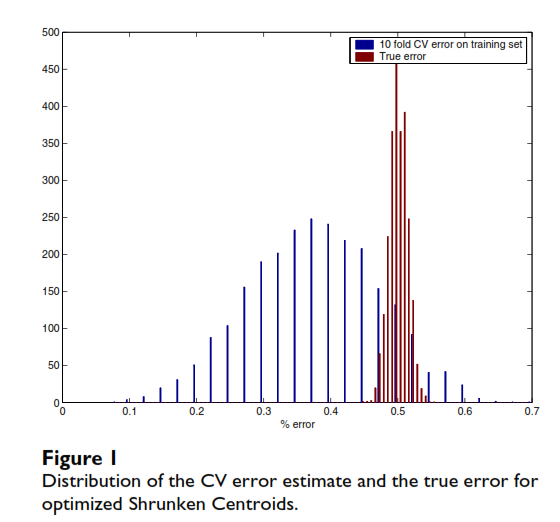
\includegraphics[keepaspectratio]{images/A-Fig1.png}}

\emph{Source: Varma \& Simon (2006), Figure 1.}

Nested cross-validation produced error estimates that were much closer
to the true error.

For the Shrunken Centroids classifier on null data:

\begin{itemize}
\tightlist
\item
  Nested CV error = 54.2\%
\item
  True error = 50.0\%
\end{itemize}

\pandocbounded{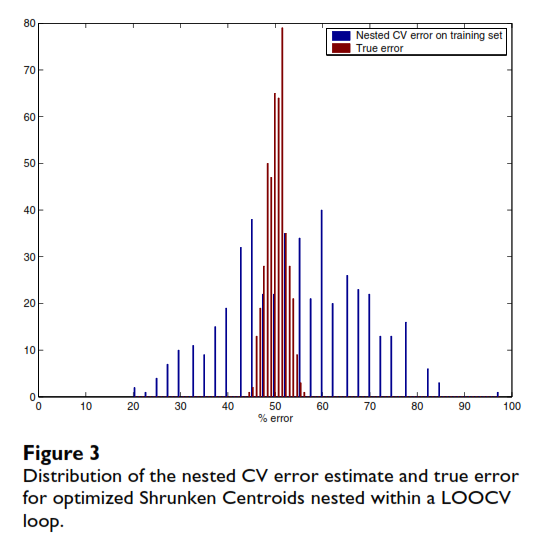
\includegraphics[keepaspectratio]{images/A-Fig3.png}}

\emph{Source: Varma \& Simon (2006), Figure 3.}

For the SVM classifier on non-null data:

\begin{itemize}
\tightlist
\item
  Nested CV error = 35.3\%
\item
  True error = 32.0\%
\end{itemize}

Their results showed that nested CV substantially reduced the bias in
the estimated prediction error.

\subsection{Main conclusion: stop doing X, start doing
Y}\label{main-conclusion-stop-doing-x-start-doing-y}

\textbf{Stop:} using the minimum cross-validation error obtained during
parameter tuning as the final estimate of how well the optimized
classifier will perform on independent data.

\textbf{Start:} treat parameter tuning as part of the training process
and use nested cross-validation, where the inner CV loop tunes the
classifier and the outer CV loop estimates prediction error.

Takeaway: Nested CV provides an almost unbiased estimate of the true
error of an optimized classifier.

\subsection{Proposed computational
exploration}\label{proposed-computational-exploration}

For my computational exploration, I plan to develop a simpler simulation
that demonstrates the parameter-selection bias described in the paper.

I will simulate a binary classification problem with two equally sized
classes and no true difference in the predictor distributions between
the classes. Therefore, the true classification error should be
approximately 50\%.

I will use a k-nearest neighbors (kNN) classifier and treat the number
of neighbors, k, as the tuning parameter. Each simulated training
dataset will contain 40 observations, with 20 observations in each
class. I will compare several candidate values of k (for example, 1, 3,
5, 7, and 9). Then, I will:

\begin{enumerate}
\def\labelenumi{\arabic{enumi}.}
\tightlist
\item
  Generate a training dataset of 40 observations from two equally sized
  classes with no true difference in their predictor distributions.
\item
  Use 10-fold cross-validation to compare several values of k and select
  the value with the lowest CV error.
\item
  Record this minimum CV error.
\item
  Use nested cross-validation with 10-fold CV in the inner loop to
  select k and LOOCV in the outer loop to estimate prediction error.
\item
  Select k using 10-fold CV on the full training dataset, train the
  optimized classifier on all 40 observations, and evaluate it on a
  large independently simulated test dataset to approximate the true
  prediction error.
\item
  Repeat the simulation 500 times and compare the distributions of the
  three error estimates.
\end{enumerate}

The main question will be whether the minimum CV error after tuning
systematically underestimates the true prediction error, and whether
nested CV produces an estimate closer to the truth.

\subsection{Planned figure}\label{planned-figure}

I plan to create a figure comparing the prediction-error estimates
obtained from:

\begin{enumerate}
\def\labelenumi{\arabic{enumi}.}
\tightlist
\item
  Minimum CV error after tuning
\item
  Nested CV
\item
  Independent test-set error
\end{enumerate}

The figure will summarize the distribution of these errors across
repeated simulations.

Because the simulated data will contain no true class difference, the
independent test-set error should be approximately 50\%. A persuasive
result would show that the minimum CV error after tuning tends to
underestimate this true error, while the nested-CV error remains closer
to it.

\subsection{Computational exploration}\label{computational-exploration}

\subsubsection{Phase 1: Simulating the
data}\label{phase-1-simulating-the-data}

I first simulate a binary classification problem with 40 observations
that are equally divided between classes A and B. The two predictors are
generated from the same distribution for both classes, so they contain
no true information about class membership. This creates a null setting
in which the expected classification error is approximately 50\%.

\begin{Shaded}
\begin{Highlighting}[]
\NormalTok{class }\OtherTok{\textless{}{-}} \FunctionTok{factor}\NormalTok{(}\FunctionTok{rep}\NormalTok{(}\FunctionTok{c}\NormalTok{(}\StringTok{"A"}\NormalTok{, }\StringTok{"B"}\NormalTok{), }\AttributeTok{each =} \DecValTok{20}\NormalTok{)) }\CommentTok{\# Creates 40 class labels: 20 A and 20 B}

\FunctionTok{table}\NormalTok{(class)}
\end{Highlighting}
\end{Shaded}

\begin{verbatim}
class
 A  B 
20 20 
\end{verbatim}

The class counts confirm that the simulated dataset is balanced, with 20
observations in class A and 20 in class B.

Next, I generate two continuous predictors, \texttt{x1} and \texttt{x2},
from a standard normal distribution with mean 0 and standard deviation
1. Because both classes use the same distribution, the predictors
contain no true class information and any apparent separation is due to
chance.

Mathematically, for each predictor \(j=1,2\),

\[
X_{ij} \mid Y_i=A \sim N(0,1)
\qquad \text{and} \qquad
X_{ij} \mid Y_i=B \sim N(0,1).
\]

\begin{Shaded}
\begin{Highlighting}[]
\FunctionTok{set.seed}\NormalTok{(}\DecValTok{123}\NormalTok{) }\CommentTok{\# Keeps data reproducible}

\NormalTok{x1 }\OtherTok{\textless{}{-}} \FunctionTok{rnorm}\NormalTok{(}\DecValTok{40}\NormalTok{, }\AttributeTok{mean =} \DecValTok{0}\NormalTok{, }\AttributeTok{sd =} \DecValTok{1}\NormalTok{) }\CommentTok{\# Generates one x1 value per observation from N(0,1)}
\NormalTok{x2 }\OtherTok{\textless{}{-}} \FunctionTok{rnorm}\NormalTok{(}\DecValTok{40}\NormalTok{, }\AttributeTok{mean =} \DecValTok{0}\NormalTok{, }\AttributeTok{sd =} \DecValTok{1}\NormalTok{) }\CommentTok{\# Generates one x2 value per observation from N(0,1)}
\end{Highlighting}
\end{Shaded}

Each observation can now be represented by its predictor vector
\(\mathbf{X}_i\) and class label \(Y_i\), where

\[
\mathbf{X}_i = (X_{i1}, X_{i2}) \in \mathbb{R}^2,
\qquad
Y_i \in \{A,B\}.
\]

Here, \(\mathbf{X}_i\) contains the two predictor values for observation
\(i\), while \(Y_i\) indicates whether that observation belongs to class
A or B. The full simulated dataset, denoted by \(\mathcal{D}\), can
therefore be written as

\[
\mathcal{D} = \{(\mathbf{X}_i, Y_i)\}_{i=1}^{40}.
\]

I combine these values into a data frame so that each row represents one
simulated observation.

\begin{Shaded}
\begin{Highlighting}[]
\NormalTok{sim\_data }\OtherTok{\textless{}{-}} \FunctionTok{data.frame}\NormalTok{(}
  \AttributeTok{class =}\NormalTok{ class,}
  \AttributeTok{x1 =}\NormalTok{ x1,}
  \AttributeTok{x2 =}\NormalTok{ x2}
\NormalTok{) }\CommentTok{\# Creates the simulated data frame}
\end{Highlighting}
\end{Shaded}

At this point, each of the 40 observations has a class label and two
predictor values, but the predictors were generated independently of
class.

To visualize the null setting, I plot \texttt{x1} against \texttt{x2}
and distinguish the two classes by color.

\begin{Shaded}
\begin{Highlighting}[]
\FunctionTok{plot}\NormalTok{(}
\NormalTok{  sim\_data}\SpecialCharTok{$}\NormalTok{x1,}
\NormalTok{  sim\_data}\SpecialCharTok{$}\NormalTok{x2,}
  \AttributeTok{col =} \FunctionTok{c}\NormalTok{(}\StringTok{"steelblue"}\NormalTok{, }\StringTok{"tomato"}\NormalTok{)[sim\_data}\SpecialCharTok{$}\NormalTok{class],}
  \AttributeTok{pch =} \DecValTok{19}\NormalTok{,}
  \AttributeTok{cex =} \FloatTok{1.2}\NormalTok{,}
  \AttributeTok{xlab =} \StringTok{"Predictor x1"}\NormalTok{,}
  \AttributeTok{ylab =} \StringTok{"Predictor x2"}\NormalTok{,}
  \AttributeTok{main =} \StringTok{"Null Simulation: No True Class Separation"}
\NormalTok{)}

\FunctionTok{legend}\NormalTok{(}
  \StringTok{"topright"}\NormalTok{,}
  \AttributeTok{legend =} \FunctionTok{c}\NormalTok{(}\StringTok{"Class A"}\NormalTok{, }\StringTok{"Class B"}\NormalTok{),}
  \AttributeTok{col =} \FunctionTok{c}\NormalTok{(}\StringTok{"steelblue"}\NormalTok{, }\StringTok{"tomato"}\NormalTok{),}
  \AttributeTok{pch =} \DecValTok{19}\NormalTok{,}
  \AttributeTok{bty =} \StringTok{"n"}
\NormalTok{)}
\end{Highlighting}
\end{Shaded}

\pandocbounded{\includegraphics[keepaspectratio]{01-cross-validation-selection-bias_files/figure-pdf/unnamed-chunk-4-1.pdf}}

The two classes overlap substantially, with no clear separation between
A and B. This is consistent with the way the data were simulated: the
predictors contain no true class signal.

\subsubsection{Phase 2: k-nearest neighbors
classification}\label{phase-2-k-nearest-neighbors-classification}

I next use k-nearest neighbors (kNN) to classify the observations. kNN
predicts the class of a new observation by finding the \(k\)
observations in the training data that are closest to it and assigning
the class that is most common among those neighbors.

Because there are two predictors, the distance between two observations
can be calculated using Euclidean distance:

\[
d(\mathbf{X}_i,\mathbf{X}_j)
=
\sqrt{(X_{i1}-X_{j1})^2 + (X_{i2}-X_{j2})^2}.
\]

Smaller values of \(k\) make the classifier depend on fewer nearby
observations, while larger values use more neighbors. I compare five
possible values of \(k\):

\[
\mathcal{K} = \{1,3,5,7,9\}.
\]

\begin{Shaded}
\begin{Highlighting}[]
\FunctionTok{library}\NormalTok{(class) }\CommentTok{\# Loads the package containing the knn() function}

\NormalTok{k\_values }\OtherTok{\textless{}{-}} \FunctionTok{c}\NormalTok{(}\DecValTok{1}\NormalTok{, }\DecValTok{3}\NormalTok{, }\DecValTok{5}\NormalTok{, }\DecValTok{7}\NormalTok{, }\DecValTok{9}\NormalTok{) }\CommentTok{\# Candidate values of k}

\NormalTok{x }\OtherTok{\textless{}{-}}\NormalTok{ sim\_data[, }\FunctionTok{c}\NormalTok{(}\StringTok{"x1"}\NormalTok{, }\StringTok{"x2"}\NormalTok{)] }\CommentTok{\# Keeps only the predictors used by kNN}
\end{Highlighting}
\end{Shaded}

\subsubsection{Phase 3: Choosing k with
cross-validation}\label{phase-3-choosing-k-with-cross-validation}

To compare the candidate values of \(k\), I use 10-fold
cross-validation. The 40 observations are divided into 10 folds, with
each fold containing two observations from class A and two from class B.

\begin{Shaded}
\begin{Highlighting}[]
\FunctionTok{set.seed}\NormalTok{(}\DecValTok{456}\NormalTok{) }\CommentTok{\# Makes the random fold assignment reproducible}

\NormalTok{fold\_id }\OtherTok{\textless{}{-}} \FunctionTok{integer}\NormalTok{(}\DecValTok{40}\NormalTok{) }\CommentTok{\# Creates a vector with one position for each observation}

\NormalTok{fold\_id[class }\SpecialCharTok{==} \StringTok{"A"}\NormalTok{] }\OtherTok{\textless{}{-}} \FunctionTok{sample}\NormalTok{(}\FunctionTok{rep}\NormalTok{(}\DecValTok{1}\SpecialCharTok{:}\DecValTok{10}\NormalTok{, }\AttributeTok{each =} \DecValTok{2}\NormalTok{))}
\NormalTok{fold\_id[class }\SpecialCharTok{==} \StringTok{"B"}\NormalTok{] }\OtherTok{\textless{}{-}} \FunctionTok{sample}\NormalTok{(}\FunctionTok{rep}\NormalTok{(}\DecValTok{1}\SpecialCharTok{:}\DecValTok{10}\NormalTok{, }\AttributeTok{each =} \DecValTok{2}\NormalTok{))}
\CommentTok{\# Randomly assigns each class across 10 folds, with 2 A and 2 B per fold}
\end{Highlighting}
\end{Shaded}

Each observation is now assigned to one of the 10 folds. During
cross-validation, one fold is held out for testing while the remaining
nine folds are used for training. This process is repeated until every
fold has served as the test fold.

To compare the candidate values of \(k\), I need to store the
cross-validation error calculated for each one.

\begin{Shaded}
\begin{Highlighting}[]
\NormalTok{cv\_error }\OtherTok{\textless{}{-}} \FunctionTok{numeric}\NormalTok{(}\FunctionTok{length}\NormalTok{(k\_values)) }\CommentTok{\# Creates space to store one CV error for each value of k}
\end{Highlighting}
\end{Shaded}

For each candidate value of \(k\), I estimate its classification error
using the 10 folds. Within each fold, the model is trained on 36
observations and tested on the 4 observations that were held out.

For a given fold, the classification error is the proportion of held-out
observations that are classified incorrectly:

\[
\widehat{\mathrm{Err}}_{f}(k)
=
\frac{1}{n_f}
\sum_{i \in f} I(\widehat{Y}_i \neq Y_i),
\]

where \(n_f\) is the number of observations in fold \(f\), and
\(I(\widehat{Y}_i \neq Y_i)\) equals 1 when an observation is classified
incorrectly and 0 when it is classified correctly.

The 10-fold cross-validation error for a given value of \(k\) is then
the average error across the 10 folds:

\[
\widehat{\mathrm{Err}}_{\mathrm{CV}}(k)
=
\frac{1}{10}
\sum_{f=1}^{10}
\widehat{\mathrm{Err}}_{f}(k).
\]

\begin{Shaded}
\begin{Highlighting}[]
\ControlFlowTok{for}\NormalTok{ (j }\ControlFlowTok{in} \FunctionTok{seq\_along}\NormalTok{(k\_values)) \{ }\CommentTok{\# Repeats once for each candidate value of k}
  
\NormalTok{  fold\_error }\OtherTok{\textless{}{-}} \FunctionTok{numeric}\NormalTok{(}\DecValTok{10}\NormalTok{) }\CommentTok{\# Stores one error for each of the 10 folds}
  
  \ControlFlowTok{for}\NormalTok{ (fold }\ControlFlowTok{in} \DecValTok{1}\SpecialCharTok{:}\DecValTok{10}\NormalTok{) \{ }\CommentTok{\# Repeats the process for each fold}
    
\NormalTok{    train\_idx }\OtherTok{\textless{}{-}}\NormalTok{ fold\_id }\SpecialCharTok{!=}\NormalTok{ fold }\CommentTok{\# Observations used for training}
\NormalTok{    test\_idx  }\OtherTok{\textless{}{-}}\NormalTok{ fold\_id }\SpecialCharTok{==}\NormalTok{ fold }\CommentTok{\# Observations held out for testing}
    
\NormalTok{    pred }\OtherTok{\textless{}{-}} \FunctionTok{knn}\NormalTok{(}
      \AttributeTok{train =}\NormalTok{ x[train\_idx, ],}
      \AttributeTok{test =}\NormalTok{ x[test\_idx, ],}
      \AttributeTok{cl =}\NormalTok{ class[train\_idx],}
      \AttributeTok{k =}\NormalTok{ k\_values[j]}
\NormalTok{    )}
    
\NormalTok{    fold\_error[fold] }\OtherTok{\textless{}{-}} \FunctionTok{mean}\NormalTok{(pred }\SpecialCharTok{!=}\NormalTok{ class[test\_idx]) }\CommentTok{\# Error in the held{-}out fold}
\NormalTok{  \}}
  
\NormalTok{  cv\_error[j] }\OtherTok{\textless{}{-}} \FunctionTok{mean}\NormalTok{(fold\_error) }\CommentTok{\# Average error across all 10 folds}
\NormalTok{\}}
\end{Highlighting}
\end{Shaded}

For each candidate value of \(k\), the model is evaluated across all 10
folds. The errors from the 10 folds are then averaged to produce one
cross-validation error for that value of \(k\). This process is repeated
for each candidate value of \(k\).

I combine the candidate values of \(k\) and their corresponding
cross-validation errors into a table so that their performance can be
compared directly.

\begin{Shaded}
\begin{Highlighting}[]
\NormalTok{cv\_results }\OtherTok{\textless{}{-}} \FunctionTok{data.frame}\NormalTok{(}
  \AttributeTok{k =}\NormalTok{ k\_values,}
  \AttributeTok{cv\_error =}\NormalTok{ cv\_error}
\NormalTok{) }\CommentTok{\# Combines each candidate k with its corresponding 10{-}fold CV error}

\NormalTok{cv\_results }\CommentTok{\# Shows the CV error for each k}
\end{Highlighting}
\end{Shaded}

\begin{verbatim}
  k cv_error
1 1    0.525
2 3    0.425
3 5    0.525
4 7    0.525
5 9    0.575
\end{verbatim}

Among the five candidate values, k = 3 has the lowest cross-validation
error at 0.425, meaning that 42.5\% of the held-out observations were
misclassified on average.

I select the value of \(k\) with the smallest cross-validation error.
This can be written as

\[
k^*
=
\underset{k \in \mathcal{K}}{\arg\min}
\ \widehat{\mathrm{Err}}_{\mathrm{CV}}(k).
\]

Here, \(k^*\) represents the value of \(k\) that appears to perform best
according to cross-validation.

\begin{Shaded}
\begin{Highlighting}[]
\NormalTok{best\_index }\OtherTok{\textless{}{-}} \FunctionTok{which.min}\NormalTok{(cv\_error) }\CommentTok{\# Finds the position of the smallest CV error}

\NormalTok{best\_k }\OtherTok{\textless{}{-}}\NormalTok{ k\_values[best\_index] }\CommentTok{\# Uses that position to identify the corresponding k}

\NormalTok{best\_k}
\end{Highlighting}
\end{Shaded}

\begin{verbatim}
[1] 3
\end{verbatim}

\begin{Shaded}
\begin{Highlighting}[]
\NormalTok{min\_cv\_error }\OtherTok{\textless{}{-}} \FunctionTok{min}\NormalTok{(cv\_error) }\CommentTok{\# Stores the lowest 10{-}fold CV error across all candidate k values}

\NormalTok{min\_cv\_error}
\end{Highlighting}
\end{Shaded}

\begin{verbatim}
[1] 0.425
\end{verbatim}

For this particular simulated dataset, cross-validation selects k = 3,
with a minimum estimated error of 42.5\%.

\subsubsection{Phase 4: Nested
cross-validation}\label{phase-4-nested-cross-validation}

The minimum cross-validation error calculated above is based on the same
cross-validation procedure that was used to choose \(k\). Because the
best-performing value is selected from several candidates, this minimum
error may make the classifier appear better than it really is.

To separate model selection from model evaluation, I next use nested
cross-validation. The procedure has two levels:

\begin{enumerate}
\def\labelenumi{\arabic{enumi}.}
\tightlist
\item
  The \textbf{inner cross-validation} chooses the best value of \(k\).
\item
  The \textbf{outer cross-validation} evaluates the classifier using an
  observation that was not involved in choosing \(k\).
\end{enumerate}

In this simulation, the outer procedure uses leave-one-out
cross-validation (LOOCV). One of the 40 observations is held out,
leaving 39 observations for model selection. Ten-fold cross-validation
is then performed using only those 39 observations to choose \(k\). The
selected value of \(k\) is used to predict the single untouched outer
observation.

This process is repeated until every observation has been held out once.

\textbf{Illustration:} How nested cross-validation works

The diagram below shows how the inner and outer stages work together.

\includegraphics[width=2.88in,height=15.06in]{01-cross-validation-selection-bias_files/figure-latex/mermaid-figure-1.png}

Because the same 10-fold cross-validation procedure is used whenever I
need to compare candidate values of \(k\), I place this repeated
computation inside a reusable function. The function takes a training
dataset, evaluates all candidate values of \(k\), and returns both the
selected \(k\) and its minimum cross-validation error.

\begin{Shaded}
\begin{Highlighting}[]
\NormalTok{select\_k\_cv }\OtherTok{\textless{}{-}} \ControlFlowTok{function}\NormalTok{(x\_train, y\_train, k\_values) \{ }\CommentTok{\# Uses 10{-}fold CV to compare candidate values of k}
  
\NormalTok{  fold\_id }\OtherTok{\textless{}{-}} \FunctionTok{integer}\NormalTok{(}\FunctionTok{length}\NormalTok{(y\_train)) }\CommentTok{\# Creates one fold label per training observation}
  
\NormalTok{  fold\_id[y\_train }\SpecialCharTok{==} \StringTok{"A"}\NormalTok{] }\OtherTok{\textless{}{-}} \FunctionTok{sample}\NormalTok{(}
    \FunctionTok{rep}\NormalTok{(}\DecValTok{1}\SpecialCharTok{:}\DecValTok{10}\NormalTok{, }\AttributeTok{length.out =} \FunctionTok{sum}\NormalTok{(y\_train }\SpecialCharTok{==} \StringTok{"A"}\NormalTok{))}
\NormalTok{  )}
  
\NormalTok{  fold\_id[y\_train }\SpecialCharTok{==} \StringTok{"B"}\NormalTok{] }\OtherTok{\textless{}{-}} \FunctionTok{sample}\NormalTok{(}
    \FunctionTok{rep}\NormalTok{(}\DecValTok{1}\SpecialCharTok{:}\DecValTok{10}\NormalTok{, }\AttributeTok{length.out =} \FunctionTok{sum}\NormalTok{(y\_train }\SpecialCharTok{==} \StringTok{"B"}\NormalTok{))}
\NormalTok{  )}
  \CommentTok{\# Distributes observations from each class approximately evenly across the 10 folds}
  
\NormalTok{  cv\_error }\OtherTok{\textless{}{-}} \FunctionTok{numeric}\NormalTok{(}\FunctionTok{length}\NormalTok{(k\_values)) }\CommentTok{\# Stores one CV error for each candidate k}
  
  \ControlFlowTok{for}\NormalTok{ (j }\ControlFlowTok{in} \FunctionTok{seq\_along}\NormalTok{(k\_values)) \{ }\CommentTok{\# Tries each candidate value of k}
    
\NormalTok{    observation\_error }\OtherTok{\textless{}{-}} \FunctionTok{numeric}\NormalTok{(}\FunctionTok{length}\NormalTok{(y\_train)) }\CommentTok{\# Stores prediction errors for this k}
    
    \ControlFlowTok{for}\NormalTok{ (fold }\ControlFlowTok{in} \DecValTok{1}\SpecialCharTok{:}\DecValTok{10}\NormalTok{) \{ }\CommentTok{\# Uses each fold once for testing}
      
\NormalTok{      train\_idx }\OtherTok{\textless{}{-}}\NormalTok{ fold\_id }\SpecialCharTok{!=}\NormalTok{ fold }\CommentTok{\# Observations used for training}
\NormalTok{      test\_idx }\OtherTok{\textless{}{-}}\NormalTok{ fold\_id }\SpecialCharTok{==}\NormalTok{ fold }\CommentTok{\# Observations held out for testing}
      
\NormalTok{      pred }\OtherTok{\textless{}{-}} \FunctionTok{knn}\NormalTok{(}
        \AttributeTok{train =}\NormalTok{ x\_train[train\_idx, , }\AttributeTok{drop =} \ConstantTok{FALSE}\NormalTok{],}
        \AttributeTok{test =}\NormalTok{ x\_train[test\_idx, , }\AttributeTok{drop =} \ConstantTok{FALSE}\NormalTok{],}
        \AttributeTok{cl =}\NormalTok{ y\_train[train\_idx],}
        \AttributeTok{k =}\NormalTok{ k\_values[j]}
\NormalTok{      )}
      
\NormalTok{      observation\_error[test\_idx] }\OtherTok{\textless{}{-}} \FunctionTok{as.numeric}\NormalTok{(}
\NormalTok{        pred }\SpecialCharTok{!=}\NormalTok{ y\_train[test\_idx]}
\NormalTok{      ) }\CommentTok{\# Records 1 for an incorrect prediction and 0 for a correct prediction}
\NormalTok{    \}}
    
\NormalTok{    cv\_error[j] }\OtherTok{\textless{}{-}} \FunctionTok{mean}\NormalTok{(observation\_error) }\CommentTok{\# Calculates CV error for this k}
\NormalTok{  \}}
  
  \FunctionTok{list}\NormalTok{(}
    \AttributeTok{best\_k =}\NormalTok{ k\_values[}\FunctionTok{which.min}\NormalTok{(cv\_error)], }\CommentTok{\# k with the lowest CV error}
    \AttributeTok{min\_cv\_error =} \FunctionTok{min}\NormalTok{(cv\_error) }\CommentTok{\# Corresponding minimum CV error}
\NormalTok{  )}
\NormalTok{\}}
\end{Highlighting}
\end{Shaded}

The outer leave-one-out procedure is also repeated whenever nested
cross-validation is performed. I therefore place this procedure inside a
reusable function. For each held-out observation, the function uses
\texttt{select\_k\_cv()} on the remaining observations to choose \(k\),
predicts the untouched observation, and finally averages the outer
prediction errors.

\begin{Shaded}
\begin{Highlighting}[]
\NormalTok{nested\_cv\_once }\OtherTok{\textless{}{-}} \ControlFlowTok{function}\NormalTok{(x, y, k\_values) \{ }\CommentTok{\# Runs nested CV on one dataset}
  
\NormalTok{  nested\_error }\OtherTok{\textless{}{-}} \FunctionTok{numeric}\NormalTok{(}\FunctionTok{length}\NormalTok{(y)) }\CommentTok{\# Stores one outer prediction error per observation}
  
  \ControlFlowTok{for}\NormalTok{ (i }\ControlFlowTok{in} \FunctionTok{seq\_along}\NormalTok{(y)) \{ }\CommentTok{\# Holds out each observation once}
    
\NormalTok{    outer\_train\_idx }\OtherTok{\textless{}{-}} \FunctionTok{seq\_along}\NormalTok{(y) }\SpecialCharTok{!=}\NormalTok{ i }\CommentTok{\# The remaining 39 observations}
\NormalTok{    outer\_test\_idx }\OtherTok{\textless{}{-}} \FunctionTok{seq\_along}\NormalTok{(y) }\SpecialCharTok{==}\NormalTok{ i }\CommentTok{\# The one untouched observation}
    
\NormalTok{    x\_outer }\OtherTok{\textless{}{-}}\NormalTok{ x[outer\_train\_idx, , drop }\OtherTok{=} \ConstantTok{FALSE}\NormalTok{]}
\NormalTok{    y\_outer }\OtherTok{\textless{}{-}}\NormalTok{ y[outer\_train\_idx]}
    
\NormalTok{    inner\_result }\OtherTok{\textless{}{-}} \FunctionTok{select\_k\_cv}\NormalTok{(}
      \AttributeTok{x\_train =}\NormalTok{ x\_outer,}
      \AttributeTok{y\_train =}\NormalTok{ y\_outer,}
      \AttributeTok{k\_values =}\NormalTok{ k\_values}
\NormalTok{    ) }\CommentTok{\# Chooses k using only the 39 outer{-}training observations}
    
\NormalTok{    best\_inner\_k }\OtherTok{\textless{}{-}}\NormalTok{ inner\_result}\SpecialCharTok{$}\NormalTok{best\_k }\CommentTok{\# Extracts the selected k}
    
\NormalTok{    pred\_outer }\OtherTok{\textless{}{-}} \FunctionTok{knn}\NormalTok{(}
      \AttributeTok{train =}\NormalTok{ x\_outer,}
      \AttributeTok{test =}\NormalTok{ x[outer\_test\_idx, , }\AttributeTok{drop =} \ConstantTok{FALSE}\NormalTok{],}
      \AttributeTok{cl =}\NormalTok{ y\_outer,}
      \AttributeTok{k =}\NormalTok{ best\_inner\_k}
\NormalTok{    ) }\CommentTok{\# Predicts the untouched outer observation}
    
\NormalTok{    nested\_error[i] }\OtherTok{\textless{}{-}}\NormalTok{ pred\_outer }\SpecialCharTok{!=}\NormalTok{ y[outer\_test\_idx]}
    \CommentTok{\# Records whether the outer prediction was incorrect}
\NormalTok{  \}}
  
  \FunctionTok{mean}\NormalTok{(nested\_error) }\CommentTok{\# Returns the average error across all outer predictions}
\NormalTok{\}}
\end{Highlighting}
\end{Shaded}

I now apply the nested cross-validation procedure to the original
40-observation dataset.

\begin{Shaded}
\begin{Highlighting}[]
\FunctionTok{set.seed}\NormalTok{(}\DecValTok{789}\NormalTok{) }\CommentTok{\# Makes the inner CV fold assignments reproducible}

\NormalTok{nested\_cv\_error }\OtherTok{\textless{}{-}} \FunctionTok{nested\_cv\_once}\NormalTok{(}
  \AttributeTok{x =}\NormalTok{ x,}
  \AttributeTok{y =}\NormalTok{ class,}
  \AttributeTok{k\_values =}\NormalTok{ k\_values}
\NormalTok{) }\CommentTok{\# Runs nested CV on the original simulated dataset}

\NormalTok{nested\_cv\_error}
\end{Highlighting}
\end{Shaded}

\begin{verbatim}
[1] 0.65
\end{verbatim}

The nested cross-validation error for this particular simulated dataset
is 65\%. Unlike the minimum ordinary cross-validation error, this
estimate is based on outer observations that were not used to choose
\(k\), so model selection and model evaluation are kept separate.

\subsubsection{Phase 5: Evaluating on an independent test
set}\label{phase-5-evaluating-on-an-independent-test-set}

Nested cross-validation provides an estimate of model performance using
only the original 40 observations. However, because the data are
simulated, I can also generate a large independent test set that was
never used for training or model selection.

In the null setting, the predictors contain no true class information,
so the expected classification error on new observations is
approximately 50\%. I therefore use the independent test set as a
benchmark for the error estimates obtained from cross-validation.

I generate 20,000 new observations using the same data-generating
process as before, with 10,000 observations from class A and 10,000 from
class B.

\begin{Shaded}
\begin{Highlighting}[]
\FunctionTok{set.seed}\NormalTok{(}\DecValTok{999}\NormalTok{) }\CommentTok{\# Makes the independent test set reproducible}

\NormalTok{test\_class }\OtherTok{\textless{}{-}} \FunctionTok{factor}\NormalTok{(}\FunctionTok{rep}\NormalTok{(}\FunctionTok{c}\NormalTok{(}\StringTok{"A"}\NormalTok{, }\StringTok{"B"}\NormalTok{), }\AttributeTok{each =} \DecValTok{10000}\NormalTok{)) }\CommentTok{\# Creates 20,000 balanced class labels}

\NormalTok{test\_x }\OtherTok{\textless{}{-}} \FunctionTok{data.frame}\NormalTok{(}
  \AttributeTok{x1 =} \FunctionTok{rnorm}\NormalTok{(}\DecValTok{20000}\NormalTok{, }\AttributeTok{mean =} \DecValTok{0}\NormalTok{, }\AttributeTok{sd =} \DecValTok{1}\NormalTok{),}
  \AttributeTok{x2 =} \FunctionTok{rnorm}\NormalTok{(}\DecValTok{20000}\NormalTok{, }\AttributeTok{mean =} \DecValTok{0}\NormalTok{, }\AttributeTok{sd =} \DecValTok{1}\NormalTok{)}
\NormalTok{) }\CommentTok{\# Generates two predictors with no true class signal}
\end{Highlighting}
\end{Shaded}

The model is then trained on all 40 original observations using the
value of \(k\) selected by ordinary cross-validation. It is evaluated on
the 20,000 new observations.

\begin{Shaded}
\begin{Highlighting}[]
\NormalTok{test\_pred }\OtherTok{\textless{}{-}} \FunctionTok{knn}\NormalTok{(}
  \AttributeTok{train =}\NormalTok{ x,}
  \AttributeTok{test =}\NormalTok{ test\_x,}
  \AttributeTok{cl =}\NormalTok{ class,}
  \AttributeTok{k =}\NormalTok{ best\_k}
\NormalTok{) }\CommentTok{\# Predicts the classes of the independent test observations}
\end{Highlighting}
\end{Shaded}

The independent test-set error is the proportion of the 20,000
predictions that are incorrect:

\[
\widehat{\mathrm{Err}}_{\mathrm{test}}
=
\frac{1}{20000}
\sum_{i=1}^{20000}
I(\widehat{Y}_i^{\mathrm{test}} \neq Y_i^{\mathrm{test}}).
\]

\begin{Shaded}
\begin{Highlighting}[]
\NormalTok{test\_error }\OtherTok{\textless{}{-}} \FunctionTok{mean}\NormalTok{(test\_pred }\SpecialCharTok{!=}\NormalTok{ test\_class) }\CommentTok{\# Proportion of independent test observations classified incorrectly}

\NormalTok{test\_error}
\end{Highlighting}
\end{Shaded}

\begin{verbatim}
[1] 0.498
\end{verbatim}

Because the independent test observations were not involved in either
training or selecting \(k\), this error provides a benchmark for how the
selected classifier performs on new data.

\subsubsection{Phase 6: Repeating the
simulation}\label{phase-6-repeating-the-simulation}

The results above are based on a single simulated dataset. Because a
different random sample of 40 observations could produce different
cross-validation errors, I repeat the entire simulation many times to
examine the behavior of each error estimate across repeated samples.

For each repetition, I generate a new dataset of 40 observations and
repeat the same three evaluations:

\begin{enumerate}
\def\labelenumi{\arabic{enumi}.}
\tightlist
\item
  Select \(k\) using ordinary 10-fold cross-validation and record the
  minimum CV error.
\item
  Estimate error using nested cross-validation.
\item
  Evaluate the selected model on a new independent test set of 20,000
  observations.
\end{enumerate}

Because the cross-validation procedures were defined as reusable
functions in Phase 4, I can apply them directly to each new simulated
dataset.

\begin{Shaded}
\begin{Highlighting}[]
\NormalTok{run\_one\_simulation }\OtherTok{\textless{}{-}} \ControlFlowTok{function}\NormalTok{() \{ }\CommentTok{\# Runs the entire experiment once}
  
\NormalTok{  y }\OtherTok{\textless{}{-}} \FunctionTok{factor}\NormalTok{(}\FunctionTok{rep}\NormalTok{(}\FunctionTok{c}\NormalTok{(}\StringTok{"A"}\NormalTok{, }\StringTok{"B"}\NormalTok{), }\AttributeTok{each =} \DecValTok{20}\NormalTok{))}
  \CommentTok{\# Creates 40 balanced class labels: 20 A and 20 B}
  
\NormalTok{  x\_sim }\OtherTok{\textless{}{-}} \FunctionTok{data.frame}\NormalTok{(}
    \AttributeTok{x1 =} \FunctionTok{rnorm}\NormalTok{(}\DecValTok{40}\NormalTok{, }\AttributeTok{mean =} \DecValTok{0}\NormalTok{, }\AttributeTok{sd =} \DecValTok{1}\NormalTok{),}
    \AttributeTok{x2 =} \FunctionTok{rnorm}\NormalTok{(}\DecValTok{40}\NormalTok{, }\AttributeTok{mean =} \DecValTok{0}\NormalTok{, }\AttributeTok{sd =} \DecValTok{1}\NormalTok{)}
\NormalTok{  ) }\CommentTok{\# Generates a new null dataset}
  
\NormalTok{  ordinary }\OtherTok{\textless{}{-}} \FunctionTok{select\_k\_cv}\NormalTok{(}
    \AttributeTok{x\_train =}\NormalTok{ x\_sim,}
    \AttributeTok{y\_train =}\NormalTok{ y,}
    \AttributeTok{k\_values =}\NormalTok{ k\_values}
\NormalTok{  ) }\CommentTok{\# Runs ordinary 10{-}fold CV on all 40 observations}
  
\NormalTok{  nested\_error }\OtherTok{\textless{}{-}} \FunctionTok{nested\_cv\_once}\NormalTok{(}
    \AttributeTok{x =}\NormalTok{ x\_sim,}
    \AttributeTok{y =}\NormalTok{ y,}
    \AttributeTok{k\_values =}\NormalTok{ k\_values}
\NormalTok{  ) }\CommentTok{\# Estimates error using nested cross{-}validation}
  
\NormalTok{  test\_y }\OtherTok{\textless{}{-}} \FunctionTok{factor}\NormalTok{(}\FunctionTok{rep}\NormalTok{(}\FunctionTok{c}\NormalTok{(}\StringTok{"A"}\NormalTok{, }\StringTok{"B"}\NormalTok{), }\AttributeTok{each =} \DecValTok{10000}\NormalTok{))}
  \CommentTok{\# Creates 20,000 balanced labels for independent testing}
  
\NormalTok{  test\_x }\OtherTok{\textless{}{-}} \FunctionTok{data.frame}\NormalTok{(}
    \AttributeTok{x1 =} \FunctionTok{rnorm}\NormalTok{(}\DecValTok{20000}\NormalTok{, }\AttributeTok{mean =} \DecValTok{0}\NormalTok{, }\AttributeTok{sd =} \DecValTok{1}\NormalTok{),}
    \AttributeTok{x2 =} \FunctionTok{rnorm}\NormalTok{(}\DecValTok{20000}\NormalTok{, }\AttributeTok{mean =} \DecValTok{0}\NormalTok{, }\AttributeTok{sd =} \DecValTok{1}\NormalTok{)}
\NormalTok{  ) }\CommentTok{\# Generates a new independent test set}
  
\NormalTok{  test\_pred }\OtherTok{\textless{}{-}} \FunctionTok{knn}\NormalTok{(}
    \AttributeTok{train =}\NormalTok{ x\_sim,}
    \AttributeTok{test =}\NormalTok{ test\_x,}
    \AttributeTok{cl =}\NormalTok{ y,}
    \AttributeTok{k =}\NormalTok{ ordinary}\SpecialCharTok{$}\NormalTok{best\_k}
\NormalTok{  ) }\CommentTok{\# Uses the k selected by ordinary CV}
  
\NormalTok{  test\_error }\OtherTok{\textless{}{-}} \FunctionTok{mean}\NormalTok{(test\_pred }\SpecialCharTok{!=}\NormalTok{ test\_y)}
  \CommentTok{\# Calculates the independent test{-}set error}
  
  \FunctionTok{c}\NormalTok{(}
    \AttributeTok{min\_cv\_error =}\NormalTok{ ordinary}\SpecialCharTok{$}\NormalTok{min\_cv\_error,}
    \AttributeTok{nested\_cv\_error =}\NormalTok{ nested\_error,}
    \AttributeTok{test\_error =}\NormalTok{ test\_error}
\NormalTok{  ) }\CommentTok{\# Returns the three error estimates}
\NormalTok{\}}
\end{Highlighting}
\end{Shaded}

\paragraph{Repeating the experiment 500
times}\label{repeating-the-experiment-500-times}

I now repeat the complete simulation 500 times. Each repetition
generates a new training dataset and a new independent test set,
allowing the three error estimates to be compared across repeated random
samples.

\begin{Shaded}
\begin{Highlighting}[]
\FunctionTok{set.seed}\NormalTok{(}\DecValTok{2026}\NormalTok{) }\CommentTok{\# Makes the complete repeated simulation reproducible}

\NormalTok{sim\_results }\OtherTok{\textless{}{-}} \FunctionTok{replicate}\NormalTok{(}
  \DecValTok{500}\NormalTok{,}
  \FunctionTok{run\_one\_simulation}\NormalTok{()}
\NormalTok{) }\CommentTok{\# Runs the entire experiment 500 times}

\NormalTok{sim\_results }\OtherTok{\textless{}{-}} \FunctionTok{as.data.frame}\NormalTok{(}\FunctionTok{t}\NormalTok{(sim\_results))}
\CommentTok{\# Converts the results so that each row represents one simulation}
\CommentTok{\# and each column represents one error{-}estimation method}

\FunctionTok{head}\NormalTok{(sim\_results) }\CommentTok{\# Displays the first six simulation results}
\end{Highlighting}
\end{Shaded}

\begin{verbatim}
  min_cv_error nested_cv_error test_error
1        0.425           0.450    0.49910
2        0.525           0.625    0.49565
3        0.200           0.200    0.50090
4        0.450           0.650    0.49925
5        0.550           0.675    0.50040
6        0.275           0.350    0.50140
\end{verbatim}

\subsubsection{Simulation results}\label{simulation-results}

To compare the three error estimates across the 500 simulations, I first
calculate their average values.

\begin{Shaded}
\begin{Highlighting}[]
\FunctionTok{colMeans}\NormalTok{(sim\_results) }\CommentTok{\# Calculates the average error for each method across all 500 simulations}
\end{Highlighting}
\end{Shaded}

\begin{verbatim}
   min_cv_error nested_cv_error      test_error 
      0.4210000       0.5126500       0.4998129 
\end{verbatim}

I also compare the full distributions of the three error estimates. The
dashed horizontal line represents the expected 50\% classification error
in the null setting.

\begin{Shaded}
\begin{Highlighting}[]
\FunctionTok{boxplot}\NormalTok{(}
\NormalTok{  sim\_results}\SpecialCharTok{$}\NormalTok{min\_cv\_error,}
\NormalTok{  sim\_results}\SpecialCharTok{$}\NormalTok{nested\_cv\_error,}
\NormalTok{  sim\_results}\SpecialCharTok{$}\NormalTok{test\_error,}
  \AttributeTok{names =} \FunctionTok{c}\NormalTok{(}\StringTok{"Minimum CV"}\NormalTok{, }\StringTok{"Nested CV"}\NormalTok{, }\StringTok{"Independent test"}\NormalTok{),}
  \AttributeTok{ylab =} \StringTok{"Classification error"}\NormalTok{,}
  \AttributeTok{main =} \StringTok{"Error Estimates Across 500 Simulations"}
\NormalTok{) }\CommentTok{\# Compares the distributions of the three error estimates}

\FunctionTok{abline}\NormalTok{(}\AttributeTok{h =} \FloatTok{0.50}\NormalTok{, }\AttributeTok{lty =} \DecValTok{2}\NormalTok{) }\CommentTok{\# Expected 50\% error under the null}
\end{Highlighting}
\end{Shaded}

\pandocbounded{\includegraphics[keepaspectratio]{01-cross-validation-selection-bias_files/figure-pdf/unnamed-chunk-21-1.pdf}}

\subsection{Conclusions}\label{conclusions}

Across 500 simulated null datasets, the minimum ordinary
cross-validation error averaged 42.1\%, while the independent test-set
error averaged 49.98\%. This shows that reporting the minimum CV error
after tuning made the classifier appear more accurate than it actually
was on new data.

Nested cross-validation produced an average error of 51.27\%, which was
much closer to the independent test-set error. This supports the main
point of Varma and Simon (2006): when cross-validation is used both to
tune a model and to report its performance, the minimum CV error can be
optimistically biased. In this simulation, nested cross-validation
provided an estimate closer to the independent test-set error.

In this small-sample simulation, nested cross-validation was also more
variable across repetitions. Its main advantage here was therefore
reducing bias rather than producing a more stable estimate.

\bookmarksetup{startatroot}

\chapter{The .632+ Bootstrap Method}\label{the-.632-bootstrap-method}

\section{Efron \& Tibshirani (1997)}\label{efron-tibshirani-1997}

\textbf{Title:} Improvements on Cross-Validation: The .632+ Bootstrap
Method\\
\textbf{Journal:} Journal of the American Statistical Association (JASA)

\subsection{Problem}\label{problem-1}

When a prediction model is trained on a sample of data, an important
question is how accurately it will perform on new observations that were
not used to train the model. Because the true prediction error on future
data is usually unknown, it must be estimated from the available sample.

Cross-validation is commonly used for this purpose and can provide a
nearly unbiased estimate of prediction error. However, cross-validation
estimates can have high variability, meaning that the estimated error
may change substantially across different samples drawn from the same
population.

Bootstrap methods provide another way to estimate prediction error. By
repeatedly resampling the observed data and averaging across many
bootstrap samples, they can produce more stable error estimates with
lower variability. However, this reduction in variability can come at
the cost of increased bias.

This creates a bias--variance trade-off: an estimator with very low bias
may still perform poorly if it is highly variable, while a more stable
estimator may perform better overall even if it introduces some bias.
Efron and Tibshirani therefore investigate whether bootstrap-based
methods can achieve a better balance between bias and variability when
estimating prediction error.

\pandocbounded{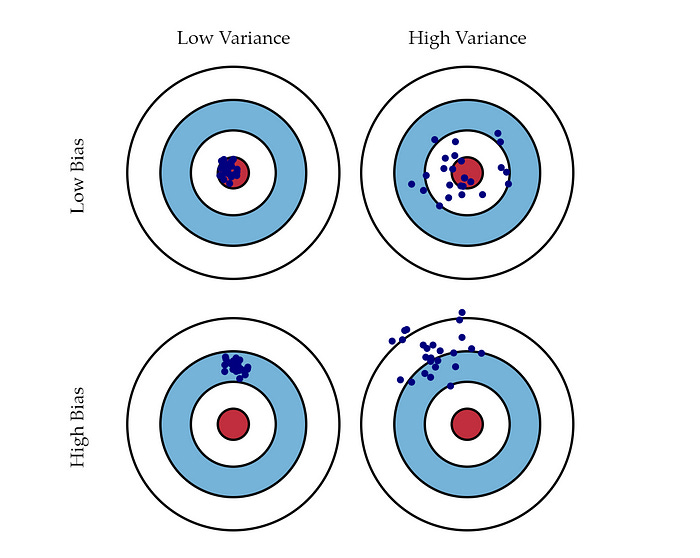
\includegraphics[keepaspectratio]{images/bias-vs-variance.jpg}}

The center of each target represents the true value. Bias describes how
far the estimates are systematically shifted away from the truth, while
variance describes how widely the estimates are spread across repeated
samples. Ideally, an estimator should have both low bias and low
variance.

\subsection{What do the authors propose
instead?}\label{what-do-the-authors-propose-instead-1}

The authors investigate bootstrap-based estimates of prediction error as
a way to reduce the high variability that can occur with
cross-validation. Their main contribution is the \textbf{.632+ bootstrap
estimator}, which attempts to combine relatively low variability with
limited bias.

A bootstrap sample is created by repeatedly sampling observations from
the original dataset \textbf{with replacement}. This means that after an
observation is selected, it remains available to be selected again. As a
result, some observations may appear several times in a bootstrap
sample, while others may not appear at all.

To illustrate, consider a very small dataset containing five
observations:

\[
\{1,2,3,4,5\}.
\]

Each bootstrap sample also contains five draws, but all five draws come
from the original observations.

\begin{Shaded}
\begin{Highlighting}[]
\FunctionTok{set.seed}\NormalTok{(}\DecValTok{632}\NormalTok{) }\CommentTok{\# Makes the bootstrap samples reproducible}

\NormalTok{original }\OtherTok{\textless{}{-}} \DecValTok{1}\SpecialCharTok{:}\DecValTok{5} \CommentTok{\# Original dataset}

\NormalTok{bootstrap\_1 }\OtherTok{\textless{}{-}} \FunctionTok{sample}\NormalTok{(original, }\AttributeTok{size =} \DecValTok{5}\NormalTok{, }\AttributeTok{replace =} \ConstantTok{TRUE}\NormalTok{)}
\NormalTok{bootstrap\_2 }\OtherTok{\textless{}{-}} \FunctionTok{sample}\NormalTok{(original, }\AttributeTok{size =} \DecValTok{5}\NormalTok{, }\AttributeTok{replace =} \ConstantTok{TRUE}\NormalTok{)}
\NormalTok{bootstrap\_3 }\OtherTok{\textless{}{-}} \FunctionTok{sample}\NormalTok{(original, }\AttributeTok{size =} \DecValTok{5}\NormalTok{, }\AttributeTok{replace =} \ConstantTok{TRUE}\NormalTok{)}

\NormalTok{bootstrap\_table }\OtherTok{\textless{}{-}} \FunctionTok{data.frame}\NormalTok{(}
  \AttributeTok{Sample =} \FunctionTok{c}\NormalTok{(}\StringTok{"Bootstrap 1"}\NormalTok{, }\StringTok{"Bootstrap 2"}\NormalTok{, }\StringTok{"Bootstrap 3"}\NormalTok{),}
  \AttributeTok{Draw\_1 =} \FunctionTok{c}\NormalTok{(bootstrap\_1[}\DecValTok{1}\NormalTok{], bootstrap\_2[}\DecValTok{1}\NormalTok{], bootstrap\_3[}\DecValTok{1}\NormalTok{]),}
  \AttributeTok{Draw\_2 =} \FunctionTok{c}\NormalTok{(bootstrap\_1[}\DecValTok{2}\NormalTok{], bootstrap\_2[}\DecValTok{2}\NormalTok{], bootstrap\_3[}\DecValTok{2}\NormalTok{]),}
  \AttributeTok{Draw\_3 =} \FunctionTok{c}\NormalTok{(bootstrap\_1[}\DecValTok{3}\NormalTok{], bootstrap\_2[}\DecValTok{3}\NormalTok{], bootstrap\_3[}\DecValTok{3}\NormalTok{]),}
  \AttributeTok{Draw\_4 =} \FunctionTok{c}\NormalTok{(bootstrap\_1[}\DecValTok{4}\NormalTok{], bootstrap\_2[}\DecValTok{4}\NormalTok{], bootstrap\_3[}\DecValTok{4}\NormalTok{]),}
  \AttributeTok{Draw\_5 =} \FunctionTok{c}\NormalTok{(bootstrap\_1[}\DecValTok{5}\NormalTok{], bootstrap\_2[}\DecValTok{5}\NormalTok{], bootstrap\_3[}\DecValTok{5}\NormalTok{]),}
  \AttributeTok{Omitted =} \FunctionTok{c}\NormalTok{(}
    \FunctionTok{paste}\NormalTok{(}\FunctionTok{setdiff}\NormalTok{(original, bootstrap\_1), }\AttributeTok{collapse =} \StringTok{", "}\NormalTok{),}
    \FunctionTok{paste}\NormalTok{(}\FunctionTok{setdiff}\NormalTok{(original, bootstrap\_2), }\AttributeTok{collapse =} \StringTok{", "}\NormalTok{),}
    \FunctionTok{paste}\NormalTok{(}\FunctionTok{setdiff}\NormalTok{(original, bootstrap\_3), }\AttributeTok{collapse =} \StringTok{", "}\NormalTok{)}
\NormalTok{  )}
\NormalTok{)}

\NormalTok{knitr}\SpecialCharTok{::}\FunctionTok{kable}\NormalTok{(}
\NormalTok{  bootstrap\_table,}
  \AttributeTok{align =} \StringTok{"c"}\NormalTok{,}
  \AttributeTok{caption =} \StringTok{"Example of bootstrap resampling with replacement"}
\NormalTok{)}
\end{Highlighting}
\end{Shaded}

\begin{longtable}[]{@{}ccccccc@{}}
\caption{Example of bootstrap resampling with
replacement}\tabularnewline
\toprule\noalign{}
Sample & Draw\_1 & Draw\_2 & Draw\_3 & Draw\_4 & Draw\_5 & Omitted \\
\midrule\noalign{}
\endfirsthead
\toprule\noalign{}
Sample & Draw\_1 & Draw\_2 & Draw\_3 & Draw\_4 & Draw\_5 & Omitted \\
\midrule\noalign{}
\endhead
\bottomrule\noalign{}
\endlastfoot
Bootstrap 1 & 2 & 5 & 1 & 1 & 2 & 3, 4 \\
Bootstrap 2 & 5 & 4 & 4 & 4 & 3 & 1, 2 \\
Bootstrap 3 & 3 & 1 & 1 & 5 & 2 & 4 \\
\end{longtable}

Although each bootstrap sample contains the same number of draws as the
original dataset, repeated observations mean that not every original
observation is necessarily represented.

For a dataset containing \(n\) observations, the probability that a
particular observation is \textbf{not} selected in one bootstrap sample
is

\[
\left(1-\frac{1}{n}\right)^n.
\]

As \(n\) becomes large, this approaches

\[
e^{-1} \approx 0.368.
\]

Therefore, approximately 36.8\% of the original observations are
expected to be left out of a bootstrap sample, while approximately

\[
1-0.368=0.632
\]

or 63.2\% are represented at least once.

The observations that are not selected in a particular bootstrap sample
were not used to train the model on that resample. They can therefore be
used to evaluate how well the fitted prediction rule performs on
observations that were left out of training.

By repeating this process across many bootstrap samples and averaging
the resulting prediction errors, the estimate becomes smoother and
generally less variable than ordinary leave-one-out cross-validation.

However, bootstrap estimation introduces another problem. Although a
bootstrap sample contains \(n\) draws, only about 63.2\% of the original
observations are represented as unique observations. The fitted model is
therefore effectively being trained on less unique information than the
model trained on the complete dataset.

Because prediction error generally increases when a model is trained on
less data, the leave-one-out bootstrap estimate can be biased upward.
Thus, bootstrap smoothing reduces variability but may introduce bias.

To correct this upward bias, Efron previously proposed the \textbf{.632
estimator}, which combines the apparent training error with the
leave-one-out bootstrap prediction error:

\[
\widehat{\mathrm{Err}}_{.632}
=
0.368\,\mathrm{err}
+
0.632\,\widehat{\mathrm{Err}}^{(1)}.
\]

Here:

\begin{itemize}
\tightlist
\item
  \(\mathrm{err}\) is the \textbf{apparent error}, obtained by
  evaluating the fitted model on the same observations used to train it.
  Because the model has already seen these observations, this error is
  generally biased downward.
\item
  \(\widehat{\mathrm{Err}}^{(1)}\) is the \textbf{leave-one-out
  bootstrap error}, estimated using observations that were omitted from
  the bootstrap samples used to fit the model.
\end{itemize}

The .632 estimator therefore combines an error estimate that tends to be
too optimistic with one that tends to be too pessimistic. It assigns
36.8\% weight to the apparent training error and 63.2\% weight to the
bootstrap error.

However, the .632 estimator can become too optimistic when the
prediction rule strongly overfits the training data.

The authors illustrate this using a no-information classification
problem in which the outcome is equally likely to belong to either of
two classes and the predictors contain no useful information about the
outcome. In this setting, the true prediction error is 50\%.

A highly flexible classifier such as 1-nearest-neighbor can nevertheless
achieve an apparent training error of

\[
\mathrm{err}=0,
\]

because each training observation is effectively able to predict itself.

If the leave-one-out bootstrap error is approximately equal to the true
no-information error of 0.50, the original .632 estimator would give

\[
\widehat{\mathrm{Err}}_{.632}
=
0.368(0)
+
0.632(0.50)
=
0.316.
\]

The estimated prediction error would therefore be only 31.6\%, even
though the true error is 50\%. The problem occurs because the .632
estimator always assigns 36.8\% of its weight to the apparent training
error, even when that training error is extremely optimistic because of
overfitting.

To address this problem, Efron and Tibshirani propose the \textbf{.632+
estimator}. Unlike the original .632 estimator, which always uses a
fixed bootstrap weight of 0.632, the .632+ method changes the weight
according to how strongly the fitted prediction rule appears to be
overfitting.

To quantify the amount of overfitting, the authors define a
\textbf{relative overfitting rate}, \(R\):

\[
R
=
\frac{
\widehat{\mathrm{Err}}^{(1)}-\mathrm{err}
}{
\gamma-\mathrm{err}
}.
\]

Here, \(\gamma\) represents the \textbf{no-information error rate}, or
the prediction error expected when the predictors contain no useful
information about the outcome.

The numerator,

\[
\widehat{\mathrm{Err}}^{(1)}-\mathrm{err},
\]

measures how much worse the model performs on observations that were not
used for training compared with its apparent training performance. The
denominator scales this difference relative to the error expected when
there is no useful predictive information.

Conceptually:

\begin{itemize}
\tightlist
\item
  \(R \approx 0\) indicates little evidence of overfitting.
\item
  \(R \approx 1\) indicates severe overfitting.
\end{itemize}

The .632+ estimator then uses \(R\) to determine the weight placed on
the bootstrap error:

\[
w
=
\frac{0.632}
{1-0.368R}.
\]

The final prediction-error estimate is

\[
\widehat{\mathrm{Err}}_{.632+}
=
(1-w)\mathrm{err}
+
w\widehat{\mathrm{Err}}^{(1)}.
\]

When there is little overfitting and \(R\) is close to 0, \(w\) is
approximately 0.632, so the method behaves similarly to the original
.632 estimator.

As overfitting becomes more severe and \(R\) approaches 1, \(w\)
approaches 1. The estimator therefore gives progressively less weight to
the overly optimistic training error and more weight to the bootstrap
prediction error.

The .632+ method therefore attempts to preserve the lower variability
obtained through bootstrap smoothing while reducing the optimistic bias
that can occur when a prediction rule strongly overfits the training
data.

\subsection{Study design}\label{study-design-1}

The authors evaluated the performance of the .632+ estimator using a
series of \textbf{24 sampling experiments} designed to represent
different prediction problems.

The experiments varied several characteristics of the prediction
problem, including:

\begin{itemize}
\tightlist
\item
  training sample size
\item
  number of predictors
\item
  number of outcome classes
\item
  strength of the relationship between the predictors and outcome
\item
  type of prediction rule
\end{itemize}

Twenty-one of the experiments involved binary classification, while
three involved four or more classes. Classification performance was
evaluated using \textbf{0-1 loss}, where each prediction was recorded as
either correct or incorrect.

Most of the experiments used simulated data, which allowed the authors
to know the underlying data-generating distribution and therefore
determine the true prediction error against which the different error
estimators could be compared.

The first 12 experiments were each repeated using \textbf{200
independently generated training datasets}, while the remaining 12
experiments used \textbf{50 repetitions}. This repeated-sampling design
allowed the authors to examine not only the average bias of each error
estimator, but also how much the estimates varied across different
training samples.

The experiments included both settings with useful predictive
information and \textbf{no-information settings}, in which the
predictors were independent of the outcome. In the binary no-information
experiments, the true prediction error was approximately 50\%.

The final experiments also included real classification datasets from
the UC Irvine Machine Learning Repository, allowing the methods to be
evaluated beyond completely simulated examples.

For each experiment, the authors compared several methods for estimating
prediction error, including leave-one-out cross-validation, 5-fold and
10-fold cross-validation, the leave-one-out bootstrap estimator, the
original .632 estimator, and the new .632+ estimator.

The bootstrap-based methods used \textbf{50 bootstrap replications} for
each simulated training dataset.

The performance of each error estimator was summarized using three
quantities:

\begin{itemize}
\tightlist
\item
  \textbf{Expectation (Exp):} the average estimated prediction error
  across repeated samples, which can be compared with the true error to
  assess bias.
\item
  \textbf{Standard deviation (SD):} how much the estimated prediction
  error varied across repeated samples.
\item
  \textbf{Root mean squared error (RMS):} the overall discrepancy
  between the estimated and true prediction error, reflecting both bias
  and variability.
\end{itemize}

\subsection{Classifier
implementation}\label{classifier-implementation-1}

The authors evaluated the different prediction-error estimators using
several classification rules with different levels of flexibility and
stability. This was important because the performance of
cross-validation and bootstrap error estimates can depend on the type of
prediction rule being evaluated.

The classifiers included:

\begin{itemize}
\tightlist
\item
  Fisher's linear discriminant function (LDF)
\item
  1-nearest neighbor (1-NN)
\item
  3-nearest neighbor (3-NN)
\item
  classification trees
\item
  quadratic discriminant function (QDF)
\end{itemize}

Using several different classifiers allowed the authors to examine
whether the .632+ estimator performed well across both relatively smooth
prediction rules and more flexible or unstable rules.

\subsubsection{Linear discriminant function
(LDF)}\label{linear-discriminant-function-ldf}

The \textbf{linear discriminant function (LDF)}, also known as linear
discriminant analysis, is a classification method that assigns an
observation to the class it is most likely to belong to based on its
predictor values.

Suppose an observation has \(p\) predictors:

\[
\mathbf{x}=(x_1,x_2,\ldots,x_p)^T.
\]

Here, \(\mathbf{x}\) represents the complete set of predictor values for
one observation, and \(T\) indicates that they are written as a column
vector.

LDF assumes that the predictors within each class approximately follow a
multivariate normal distribution:

\[
\mathbf{X}\mid Y=k
\sim
N_p(\boldsymbol{\mu}_k,\Sigma).
\]

In this notation:

\begin{itemize}
\tightlist
\item
  \(\boldsymbol{\mu}_k\) is the mean predictor vector for class \(k\),
  representing the typical predictor values for that class.
\item
  \(\Sigma\) is the covariance matrix, which describes the variability
  of the predictors and how they are correlated.
\item
  LDF assumes that the same covariance matrix \(\Sigma\) applies to
  every class.
\end{itemize}

For each possible class, LDF calculates a discriminant score:

\[
\delta_k(\mathbf{x})
=
\mathbf{x}^T\Sigma^{-1}\boldsymbol{\mu}_k
-
\frac{1}{2}
\boldsymbol{\mu}_k^T\Sigma^{-1}\boldsymbol{\mu}_k
+
\log(\pi_k).
\]

The components of this score can be interpreted as follows:

\begin{itemize}
\tightlist
\item
  \(\mathbf{x}^T\Sigma^{-1}\boldsymbol{\mu}_k\) measures how well the
  new observation matches the predictor profile of class \(k\), while
  accounting for predictor variability and correlation.
\item
  \(-\frac{1}{2}\boldsymbol{\mu}_k^T\Sigma^{-1}\boldsymbol{\mu}_k\)
  adjusts the score for the location of the class mean.
\item
  \(\pi_k\) is the prior probability of belonging to class \(k\), so
  \(\log(\pi_k)\) allows more common classes to receive appropriate
  weight.
\end{itemize}

The observation is assigned to the class with the largest discriminant
score:

\[
\widehat{Y}
=
\underset{k}{\arg\max}\,
\delta_k(\mathbf{x}).
\]

Here, \(\arg\max\) simply means \textbf{choose the class \(k\) that
produces the largest score}.

Because all classes are assumed to share the same covariance matrix, the
resulting decision boundary is linear. LDF therefore represents a
relatively smooth classification rule compared with more flexible
methods such as nearest-neighbor classification.

\subsubsection{1-nearest neighbor}\label{nearest-neighbor}

The \textbf{1-nearest-neighbor (1-NN)} classifier predicts the class of
a new observation by finding the most similar observation in the
training dataset.

Similarity is usually measured using \textbf{Euclidean distance}:

\[
d(\mathbf{x}_i,\mathbf{x}_j)
=
\sqrt{
\sum_{m=1}^{p}
(x_{im}-x_{jm})^2
}.
\]

Here:

\begin{itemize}
\tightlist
\item
  \(\mathbf{x}_i\) and \(\mathbf{x}_j\) are two observations.
\item
  \(p\) is the number of predictors.
\item
  \(x_{im}\) is the value of predictor \(m\) for observation \(i\).
\item
  \(x_{jm}\) is the value of predictor \(m\) for observation \(j\).
\item
  For each predictor, the difference between the two observations is
  squared.
\item
  These squared differences are added together and the square root is
  taken.
\end{itemize}

For example, if there are two predictors and the observations are

\[
\mathbf{x}_i=(2,3)
\qquad\text{and}\qquad
\mathbf{x}_j=(5,7),
\]

then

\[
d(\mathbf{x}_i,\mathbf{x}_j)
=
\sqrt{(2-5)^2+(3-7)^2}
=
\sqrt{9+16}
=
5.
\]

For a new observation \(\mathbf{x}_0\), 1-NN compares its distance with
every observation in the training dataset and identifies the one with
the smallest distance:

\[
j^*
=
\underset{j}{\arg\min}\,
d(\mathbf{x}_0,\mathbf{x}_j).
\]

Here, \(\arg\min\) means \textbf{choose the training observation \(j\)
that gives the smallest distance}. The symbol \(j^*\) therefore
represents the index of the nearest training observation.

The new observation is then assigned the same class as that nearest
neighbor:

\[
\widehat{Y}_0=Y_{j^*}.
\]

Here:

\begin{itemize}
\tightlist
\item
  \(\widehat{Y}_0\) is the predicted class for the new observation.
\item
  \(Y_{j^*}\) is the actual class of its nearest training observation.
\end{itemize}

Unlike LDF, 1-NN can create highly irregular decision boundaries because
its prediction can change whenever a different training observation
becomes the closest one.

\subsubsection{3-nearest neighbor}\label{nearest-neighbor-1}

The \textbf{3-nearest-neighbor (3-NN)} classifier follows the same
general principle as 1-NN but uses the three closest training
observations rather than only one.

For a new observation \(\mathbf{x}_0\), the distance to every training
observation is calculated in the same way as for 1-NN. The three
observations with the smallest distances are then selected.

The predicted class is determined by \textbf{majority vote} among those
three neighbors.

For example, if the three nearest observations belong to

\[
\{A,A,B\},
\]

then two of the three neighbors belong to class \(A\), so the prediction
is

\[
\widehat{Y}_0=A.
\]

In general, 3-NN can be thought of as assigning the new observation to
the class that appears most frequently among its three nearest
neighbors.

Because the prediction depends on several nearby observations instead of
only one, 3-NN is generally less sensitive to a single unusual training
observation and therefore smoother than 1-NN.

However, it remains a local and relatively flexible prediction rule
because the classification still depends heavily on the observations
located near the new data point.

Including both 1-NN and 3-NN allowed the authors to examine how the
prediction-error estimators behaved when the flexibility of the
nearest-neighbor classifier changed.

\subsubsection{Quadratic discriminant function
(QDF)}\label{quadratic-discriminant-function-qdf}

The \textbf{quadratic discriminant function (QDF)} is closely related to
LDF, but it makes a less restrictive assumption about how the predictors
vary within each class.

LDF assumes that all classes share the same covariance matrix:

\[
\mathbf{X}\mid Y=k
\sim
N_p(\boldsymbol{\mu}_k,\Sigma).
\]

QDF instead allows each class to have its own covariance matrix:

\[
\mathbf{X}\mid Y=k
\sim
N_p(\boldsymbol{\mu}_k,\Sigma_k).
\]

Here:

\begin{itemize}
\tightlist
\item
  \(\boldsymbol{\mu}_k\) is the mean predictor vector for class \(k\).
\item
  \(\Sigma_k\) is the covariance matrix for class \(k\).
\item
  The subscript \(k\) indicates that the pattern of variability and
  correlation between predictors is allowed to differ across classes.
\end{itemize}

For each possible class, QDF calculates a discriminant score:

\[
\delta_k(\mathbf{x})
=
-\frac{1}{2}\log|\Sigma_k|
-\frac{1}{2}
(\mathbf{x}-\boldsymbol{\mu}_k)^T
\Sigma_k^{-1}
(\mathbf{x}-\boldsymbol{\mu}_k)
+
\log(\pi_k).
\]

The main components can be interpreted as follows:

\begin{itemize}
\tightlist
\item
  \((\mathbf{x}-\boldsymbol{\mu}_k)\) measures how far the new
  observation is from the mean of class \(k\).
\item
  \(\Sigma_k^{-1}\) adjusts that distance for the variability and
  correlations within class \(k\).
\item
  \(|\Sigma_k|\) is the determinant of the covariance matrix and
  reflects the overall spread of the class distribution.
\item
  \(\pi_k\) is the prior probability of belonging to class \(k\).
\end{itemize}

The observation is assigned to the class with the largest discriminant
score:

\[
\widehat{Y}
=
\underset{k}{\arg\max}\,
\delta_k(\mathbf{x}).
\]

As before, \(\arg\max\) simply means \textbf{choose the class that
produces the largest score}.

The key difference from LDF is that QDF allows \(\Sigma_k\) to differ
between classes. Because the covariance structure is no longer shared,
the quadratic terms do not cancel, and the resulting decision boundary
can be curved rather than linear.

QDF is therefore more flexible than LDF, but it also requires estimating
more parameters from the training data.

\subsubsection{Why use several different
classifiers?}\label{why-use-several-different-classifiers}

The classifiers used in the experiments represent prediction rules with
different levels of smoothness, flexibility, and stability.

{\def\LTcaptype{none} % do not increment counter
\begin{longtable}[]{@{}ll@{}}
\toprule\noalign{}
Prediction rule & General behavior \\
\midrule\noalign{}
\endhead
\bottomrule\noalign{}
\endlastfoot
LDF & Relatively smooth, linear decision boundary \\
1-NN & Highly local and flexible \\
3-NN & Local but smoother than 1-NN \\
Classification tree & Flexible and potentially unstable \\
QDF & More flexible discriminant rule with quadratic boundaries \\
\end{longtable}
}

This diversity was important because the authors were not only
interested in whether .632+ worked for one particular classifier. They
wanted to determine whether its bias and variability advantages remained
useful across prediction problems with substantially different types of
prediction rules.

Using classifiers with different levels of flexibility also allowed the
authors to examine how the error estimators behaved when the underlying
prediction rule was more or less prone to overfitting or instability.

\subsection{Bootstrap implementation}\label{bootstrap-implementation}

For each training dataset, the authors generated multiple bootstrap
samples and used them to estimate prediction error. In the simulation
experiments, each bootstrap-based estimate used

\[
B = 50
\]

bootstrap replications.

Each bootstrap sample contained \(n\) draws with replacement from the
original training dataset of \(n\) observations. Because sampling is
performed with replacement, some observations may appear multiple times
in a bootstrap sample, while others may not appear at all.

The prediction rule was fitted separately to each bootstrap sample.

The important feature of the procedure is that an original observation
was evaluated only using bootstrap samples in which that observation had
\textbf{not} been selected. This ensures that the observation being
tested was not used to train that particular model.

Suppose the original training dataset is

\[
\mathcal{D}
=
\{(\mathbf{x}_i,y_i)\}_{i=1}^{n},
\]

where \(\mathbf{x}_i\) represents the predictor values for observation
\(i\) and \(y_i\) represents its true class.

Let

\[
\mathcal{D}^{*b}
\]

represent bootstrap sample \(b\), where

\[
b=1,\ldots,B.
\]

The asterisk indicates that this is a resampled version of the original
dataset, and \(b\) identifies which bootstrap replication is being
considered.

For each original observation \(i\), define

\[
I_i^b
=
\begin{cases}
1, & \text{if observation } i \text{ is absent from bootstrap sample } b,\\
0, & \text{if observation } i \text{ is included in bootstrap sample } b.
\end{cases}
\]

Thus, \(I_i^b\) tells us whether observation \(i\) can be used as a test
observation for bootstrap sample \(b\).

If

\[
I_i^b=1,
\]

the model fitted using bootstrap sample \(b\) is used to predict
observation \(i\).

For classification with 0-1 loss, define the prediction error as

\[
Q_i^b
=
\begin{cases}
1, & \text{if the model predicts observation } i \text{ incorrectly},\\
0, & \text{if the prediction is correct}.
\end{cases}
\]

For each original observation, the prediction errors are then averaged
across only the bootstrap samples in which that observation was omitted:

\[
\widehat{e}_i
=
\frac{
\sum_{b=1}^{B} I_i^b Q_i^b
}{
\sum_{b=1}^{B} I_i^b
}.
\]

The numerator,

\[
\sum_{b=1}^{B} I_i^b Q_i^b,
\]

counts the prediction errors for observation \(i\) across bootstrap
samples in which it was left out.

The denominator,

\[
\sum_{b=1}^{B} I_i^b,
\]

counts how many bootstrap samples left observation \(i\) out.

Their ratio therefore represents the average prediction error for
observation \(i\) when it was evaluated using models that had not been
trained on it.

Finally, these observation-specific errors are averaged across all \(n\)
original observations:

\[
\widehat{\mathrm{Err}}^{(1)}
=
\frac{1}{n}
\sum_{i=1}^{n}
\widehat{e}_i.
\]

This gives the \textbf{leave-one-out bootstrap error}.

Conceptually, this procedure is similar to cross-validation because an
observation is evaluated only by models that were trained without that
observation. The difference is that bootstrap estimation repeatedly
resamples the training dataset with replacement and averages prediction
errors across many different resampled training sets.

The complete bootstrap procedure can therefore be summarized as:

\begin{enumerate}
\def\labelenumi{\arabic{enumi}.}
\tightlist
\item
  Draw a bootstrap sample of size \(n\) from the original training
  dataset with replacement.
\item
  Fit the prediction rule using that bootstrap sample.
\item
  Identify the original observations that were not selected in the
  bootstrap sample.
\item
  Use the fitted model to predict those omitted observations.
\item
  Record whether each prediction is correct or incorrect.
\item
  Repeat the process for \(B=50\) bootstrap samples.
\item
  For each original observation, average its prediction errors across
  the bootstrap samples in which it was omitted.
\item
  Average these observation-level errors to obtain
  \(\widehat{\mathrm{Err}}^{(1)}\).
\end{enumerate}

\includegraphics[width=2.88in,height=13.48in]{02-632-plus-bootstrap_files/figure-latex/mermaid-figure-1.png}

Once \(\widehat{\mathrm{Err}}^{(1)}\) has been calculated, it can be
combined with the apparent training error to obtain the original .632
estimate:

\[
\widehat{\mathrm{Err}}_{.632}
=
0.368\,\mathrm{err}
+
0.632\,\widehat{\mathrm{Err}}^{(1)}.
\]

Here:

\begin{itemize}
\tightlist
\item
  \(\mathrm{err}\) is the \textbf{apparent training error}, calculated
  on the same observations used to fit the model.
\item
  \(\widehat{\mathrm{Err}}^{(1)}\) is the \textbf{leave-one-out
  bootstrap error}, calculated using observations that were omitted from
  the bootstrap samples used for training.
\end{itemize}

The apparent training error is usually optimistic, while the
leave-one-out bootstrap error can be somewhat pessimistic. The .632
estimator combines the two, giving 36.8\% weight to the apparent
training error and 63.2\% weight to the bootstrap error.

However, this fixed weighting can still produce an overly optimistic
estimate when the model strongly overfits the training data.

To address this problem, the .632+ estimator first measures the degree
of overfitting using the \textbf{relative overfitting rate}, \(R\):

\[
R
=
\frac{
\widehat{\mathrm{Err}}^{(1)}-\mathrm{err}
}{
\gamma-\mathrm{err}
}.
\]

Here, \(\gamma\) represents the \textbf{no-information error rate}, or
the error expected if the predictors contained no useful information
about the outcome.

Conceptually:

\begin{itemize}
\tightlist
\item
  \(R\approx0\) indicates little evidence of overfitting.
\item
  \(R\approx1\) indicates severe overfitting, where performance on
  unseen observations approaches the no-information error level.
\end{itemize}

The value of \(R\) is then used to calculate an adaptive bootstrap
weight:

\[
w
=
\frac{0.632}{1-0.368R}.
\]

When there is little overfitting and \(R\) is close to 0,

\[
w\approx0.632,
\]

so the .632+ estimator behaves similarly to the original .632 estimator.

As overfitting becomes more severe and \(R\) approaches 1,

\[
w\rightarrow1.
\]

The .632+ estimator therefore places progressively more weight on the
bootstrap error and less weight on the potentially overly optimistic
training error.

The final .632+ estimate is

\[
\widehat{\mathrm{Err}}_{.632+}
=
(1-w)\mathrm{err}
+
w\widehat{\mathrm{Err}}^{(1)}.
\]

Thus, the same set of bootstrap replications first provides the
leave-one-out bootstrap error, which is then used to calculate both the
.632 and .632+ prediction-error estimates. The key difference is that
.632 uses fixed weights, whereas .632+ adapts the weights according to
the estimated degree of overfitting.

\subsection{Main findings}\label{main-findings-1}

The results showed that no single method was best in every respect.
Cross-validation tended to have relatively low bias, while
bootstrap-based methods generally produced less variable estimates of
prediction error.

\subsubsection{Bootstrap smoothing reduced
variability}\label{bootstrap-smoothing-reduced-variability}

The first important finding was that the leave-one-out bootstrap
estimate, \(\widehat{\mathrm{Err}}^{(1)}\), was consistently less
variable than leave-one-out cross-validation.

Across the 24 experiments, the median ratio of the standard deviation of
the bootstrap estimate to the standard deviation of the cross-validation
estimate was

\[
\frac{
SD\left(\widehat{\mathrm{Err}}^{(1)}\right)
}{
SD\left(\widehat{\mathrm{Err}}_{\mathrm{CV}}\right)
}
=
0.79.
\]

This means that the bootstrap error estimate typically had substantially
lower variability than leave-one-out cross-validation.

The authors noted that this reduction in variability was roughly
equivalent to increasing the training sample size by about 60\%.

\pandocbounded{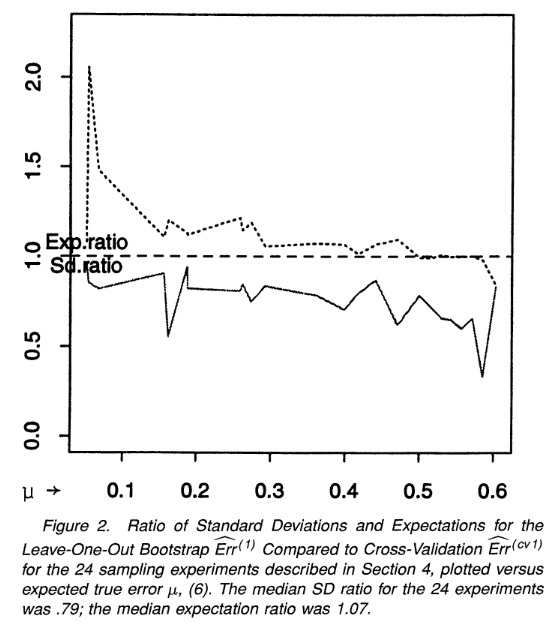
\includegraphics[keepaspectratio]{images/B-Fig2.png}}

\emph{Source: Efron \& Tibshirani (1997), Figure 2.}

However, the bootstrap estimate was not unbiased. The average bootstrap
error tended to be slightly higher than the cross-validation error,
illustrating the trade-off between reduced variability and increased
bias.

\subsubsection{The original .632 estimator could be too
optimistic}\label{the-original-.632-estimator-could-be-too-optimistic}

The original .632 estimator reduced the upward bias of the leave-one-out
bootstrap estimate by combining it with the apparent training error.

However, in prediction rules that strongly overfit the training data,
particularly nearest-neighbor classifiers, the .632 estimator could
become substantially biased downward.

This occurred because the apparent training error could be extremely
small even when prediction performance on new data was poor. The fixed
36.8\% weight placed on this optimistic training error could therefore
pull the .632 estimate too far downward.

The .632+ estimator was designed to reduce this problem by increasing
the weight placed on the bootstrap error when evidence of overfitting
was strong.

\subsubsection{.632+ improved the bias--variance
compromise}\label{improved-the-biasvariance-compromise}

Across the simulation experiments, the .632+ estimator generally
provided a compromise between the upward bias of the leave-one-out
bootstrap estimator and the downward bias that could occur with the
original .632 estimator.

\pandocbounded{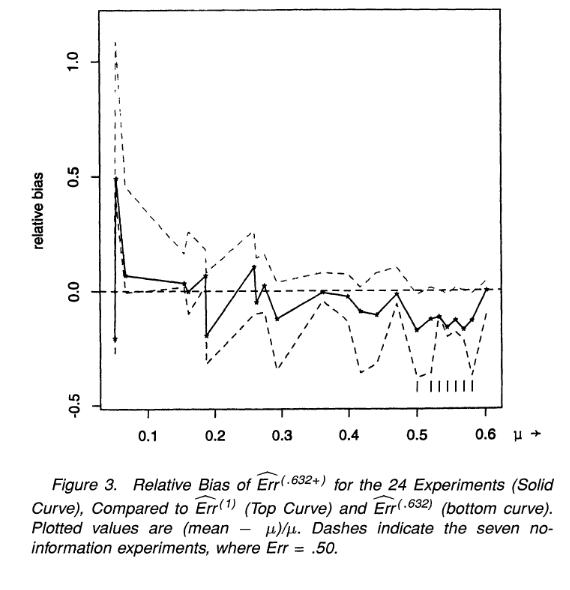
\includegraphics[keepaspectratio]{images/B-Fig3.png}}

\emph{Source: Efron \& Tibshirani (1997), Figure 3.}

The purpose of the adaptive weighting in .632+ was therefore not to
eliminate bias completely, but to prevent the strong optimistic bias
that could occur with .632 while retaining much of the reduction in
variability obtained through bootstrap smoothing.

\subsubsection{.632+ had the lowest overall estimation
error}\label{had-the-lowest-overall-estimation-error}

Because an estimator can have low bias but still perform poorly if it is
highly variable, the authors also compared the methods using root mean
squared error (RMS).

Across the 24 experiments, the .632+ estimator was the best overall
performer in terms of RMS error.

The authors compared the RMS error of .632+ with that of leave-one-out
cross-validation using

\[
\frac{
RMS\left(\widehat{\mathrm{Err}}_{.632+}\right)
}{
RMS\left(\widehat{\mathrm{Err}}_{\mathrm{CV}}\right)
}.
\]

The median value of this ratio across the 24 experiments was

\[
0.78.
\]

A value below 1 indicates that .632+ had lower RMS error than
leave-one-out cross-validation. A median ratio of 0.78 therefore
indicates that the overall estimation error of .632+ was substantially
smaller across the experiments.

\pandocbounded{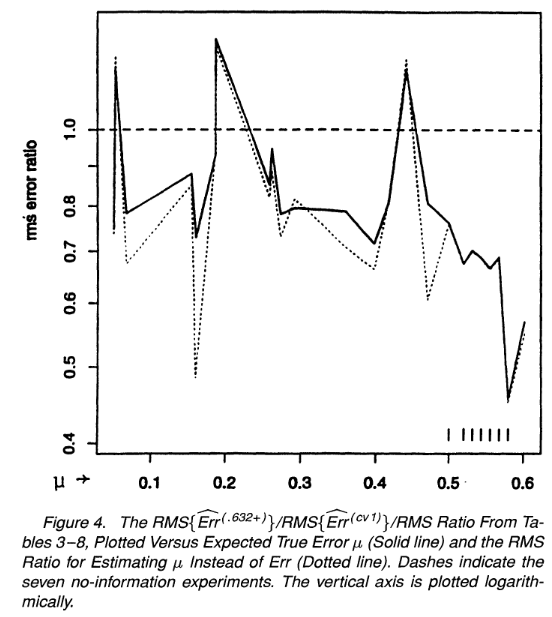
\includegraphics[keepaspectratio]{images/B-Fig4.png}}

\emph{Source: Efron \& Tibshirani (1997), Figure 4.}

Overall, the results suggest that the main advantage of .632+ was not
that it was completely unbiased. Instead, it achieved a better balance
between bias and variability, resulting in lower overall
prediction-error estimation error across a wide range of classification
problems.

\subsection{Main conclusion: stop doing X, start doing
Y}\label{main-conclusion-stop-doing-x-start-doing-y-1}

\textbf{Stop:} assuming that an approximately unbiased prediction-error
estimator is necessarily the best estimator if its estimates are highly
variable, and avoid relying on the original .632 estimator when strong
overfitting may make the apparent training error extremely optimistic.

\textbf{Start:} consider the .632+ bootstrap estimator as a way to
obtain a better balance between bias and variability, particularly when
the prediction rule may be unstable or prone to overfitting.

\textbf{Takeaway:} In the authors' simulation experiments, the .632+
estimator was the best overall performer, combining relatively low
variability with only moderate bias. Its main advantage was not that it
completely eliminated bias, but that its adaptive weighting produced a
better overall bias--variance compromise than the competing methods.

The authors nevertheless caution that these conclusions are based on a
finite set of simulation experiments and should not be interpreted as
evidence that .632+ will necessarily outperform cross-validation in
every prediction problem.

\subsection{Proposed computational
exploration}\label{proposed-computational-exploration-1}

To illustrate the main argument of Efron and Tibshirani, I will simulate
a simple \textbf{no-information binary classification problem} using a
1-nearest-neighbor classifier. This simulation is designed as a
simplified reproduction of \textbf{Experiment 8} from Efron and
Tibshirani, which used a 1-nearest-neighbor classifier with \(n=20\),
two predictors, and a no-information data-generating process in which
the true prediction error was 0.50.

Each simulated dataset will contain \(n=20\) observations and two
normally distributed predictors. The binary outcome will be generated
independently of the predictors, so there is no true predictive signal
and the true prediction error is

\[
\mathrm{Err}=0.50.
\]

For each simulated dataset, I will calculate:

\begin{itemize}
\tightlist
\item
  the apparent training error,
\item
  leave-one-out cross-validation error,
\item
  leave-one-out bootstrap error using \(B=50\) bootstrap samples,
\item
  the .632 estimate,
\item
  and the .632+ estimate.
\end{itemize}

The complete simulation will be repeated 500 times using independently
generated datasets. Repeating the experiment allows the behavior of each
prediction-error estimator to be evaluated across samples.

Following the general evaluation approach used by Efron and Tibshirani,
the estimators will be compared using:

\begin{itemize}
\tightlist
\item
  \textbf{Exp:} the average estimated prediction error across
  simulations,
\item
  \textbf{SD:} the standard deviation of the estimates across
  simulations,
\item
  \textbf{RMS:} the root mean squared error relative to the known true
  error.
\end{itemize}

Bias will also be calculated as

\[
\mathrm{Bias}
=
\mathrm{Exp}
-
\mathrm{Err},
\]

to show whether each estimator tends to overestimate or underestimate
the true prediction error.

This exploration is intended to demonstrate how strong overfitting can
make the original .632 estimator overly optimistic and how the adaptive
weighting of .632+ can improve the overall bias--variance compromise.

\subsection{Planned figure}\label{planned-figure-1}

The main figure will compare the distributions of the four
prediction-error estimators across the repeated simulations:

\[
\text{LOOCV},
\qquad
\widehat{\mathrm{Err}}^{(1)},
\qquad
\widehat{\mathrm{Err}}_{.632},
\qquad
\widehat{\mathrm{Err}}_{.632+}.
\]

A vertical reference line at

\[
\mathrm{Err}=0.50
\]

will indicate the known true prediction error. The location of each
distribution relative to this line will illustrate bias, while the
spread of each distribution will illustrate variability.

\subsection{Computational
exploration}\label{computational-exploration-1}

\subsubsection{Phase 1: Define the functions used in the
simulation}\label{phase-1-define-the-functions-used-in-the-simulation}

The computational exploration requires two functions. The first performs
prediction using a \textbf{1-nearest-neighbor (1-NN)} classifier. The
second generates one no-information dataset and calculates all
prediction-error estimates for that dataset.

\paragraph{1-NN prediction function}\label{nn-prediction-function}

For a new observation \(\mathbf{x}_0\), 1-NN compares it with every
training observation \(\mathbf{x}_j\) using Euclidean distance:

\[
d(\mathbf{x}_0,\mathbf{x}_j)
=
\sqrt{
\sum_{m=1}^{p}
(x_{0m}-x_{jm})^2
}.
\]

The nearest training observation is

\[
j^*
=
\underset{j}{\arg\min}\,
d(\mathbf{x}_0,\mathbf{x}_j),
\]

and the predicted class is

\[
\widehat{Y}_0
=
Y_{j^*}.
\]

Because taking the square root does not change which distance is
smallest, the code uses \textbf{squared Euclidean distance}:

\[
d^2(\mathbf{x}_0,\mathbf{x}_j)
=
\sum_{m=1}^{p}
(x_{0m}-x_{jm})^2.
\]

The prediction function therefore performs four steps:

\begin{enumerate}
\def\labelenumi{\arabic{enumi}.}
\tightlist
\item
  Compare the new observation with every training observation.
\item
  Calculate the squared Euclidean distance to each training observation.
\item
  Identify the observation with the smallest distance.
\item
  Assign the new observation the class of that nearest neighbor.
\end{enumerate}

\paragraph{One complete simulation}\label{one-complete-simulation}

The second function, \texttt{run\_one\_simulation()}, defines the
complete procedure that will be carried out for \textbf{one simulated
dataset}.

For each dataset, the function:

\begin{enumerate}
\def\labelenumi{\arabic{enumi}.}
\tightlist
\item
  generates \(n=20\) observations from a no-information binary
  classification problem,
\item
  calculates the apparent training error,
\item
  calculates leave-one-out cross-validation error,
\item
  calculates leave-one-out bootstrap error using \(B=50\) bootstrap
  samples,
\item
  calculates the original .632 estimate,
\item
  calculates the .632+ estimate, including \(\widehat{\gamma}\), \(R\),
  and the adaptive weight \(w\),
\item
  returns all of these quantities for that simulated dataset.
\end{enumerate}

At this stage, the function only defines how \textbf{one experiment} is
performed. In later phases, this entire function will be repeated across
500 independently generated datasets.

Repeating the experiment will allow the estimators to be compared across
samples using \textbf{Exp}, \textbf{SD}, and \textbf{RMS}, as described
in the proposed computational exploration, with the known true
prediction error

\[
\mathrm{Err}=0.50.
\]

First, two predictors are generated independently from standard normal
distributions:

\[
X_{i1},X_{i2}\sim N(0,1).
\]

The binary outcome is generated independently of the predictors:

\[
Y_i\sim\mathrm{Bernoulli}(0.50).
\]

Because the outcome is independent of the predictors, the dataset
contains \textbf{no predictive signal}. The population-level prediction
error for this balanced two-class problem is therefore

\[
\mathrm{Err}=0.50.
\]

The function then calculates the following error estimates.

\textbf{Apparent training error}

The 1-NN classifier is evaluated on the same observations used to train
it:

\[
\mathrm{err}
=
\frac{1}{n}
\sum_{i=1}^{n}
I(\widehat{Y}_i\neq Y_i).
\]

Because each training observation is its own nearest neighbor, its
distance from itself is zero. The apparent training error is therefore
expected to be approximately

\[
\mathrm{err}=0.
\]

\textbf{Leave-one-out cross-validation}

For each observation \(i\), the classifier is trained using the other
\(n-1\) observations and then used to predict the omitted observation:

\[
\widehat{\mathrm{Err}}_{\mathrm{CV}}
=
\frac{1}{n}
\sum_{i=1}^{n}
I(\widehat{Y}_i^{(-i)}\neq Y_i).
\]

Here, \(\widehat{Y}_i^{(-i)}\) represents the prediction for observation
\(i\) from a model trained without that observation.

\textbf{Leave-one-out bootstrap error}

For each of

\[
B=50
\]

bootstrap replications, \(n\) observations are sampled with replacement
from the original dataset.

The classifier is fitted to the bootstrap sample and evaluated only on
original observations that were omitted from that sample. Prediction
errors are averaged for each observation across the bootstrap samples in
which it was omitted, and these observation-level errors are then
averaged to obtain

\[
\widehat{\mathrm{Err}}^{(1)}.
\]

\textbf{Original .632 estimator}

The apparent training error and bootstrap error are combined as

\[
\widehat{\mathrm{Err}}_{.632}
=
0.368\,\mathrm{err}
+
0.632\,\widehat{\mathrm{Err}}^{(1)}.
\]

Because the apparent error for 1-NN is approximately zero in this
setting, the .632 estimate may be pulled substantially below the true
error of 0.50.

\textbf{.632+ estimator}

The .632+ estimator additionally measures the degree of overfitting.

For binary nearest-neighbor classification, the no-information error
rate can be estimated from the observed proportion of class-1 outcomes,
\(\widehat p\), using

\[
\widehat{\gamma}
=
2\widehat{p}(1-\widehat{p}).
\]

For the implementation used in the simulation experiments, the bootstrap
error is first limited by the estimated no-information error:

\[
\widehat{\mathrm{Err}}_{\mathrm{adj}}^{(1)}
=
\min\left(
\widehat{\mathrm{Err}}^{(1)},
\widehat{\gamma}
\right).
\]

The relative overfitting rate is then calculated using this adjusted
bootstrap error:

\[
R
=
\frac{
\widehat{\mathrm{Err}}_{\mathrm{adj}}^{(1)}-\mathrm{err}
}{
\widehat{\gamma}-\mathrm{err}
}.
\]

If the bootstrap error does not exceed the apparent error, \(R\) is set
to 0. Otherwise, the adjustment above keeps \(R\) between 0 and 1.

The adaptive weight is

\[
w
=
\frac{0.632}{1-0.368R},
\]

and the final estimate is

\[
\widehat{\mathrm{Err}}_{.632+}
=
(1-w)\mathrm{err}
+
w\widehat{\mathrm{Err}}_{\mathrm{adj}}^{(1)}.
\]

As overfitting becomes more severe, \(R\) approaches 1 and \(w\)
approaches 1. The .632+ estimator therefore places progressively less
weight on the overly optimistic apparent training error.

\begin{Shaded}
\begin{Highlighting}[]
\NormalTok{predict\_1nn }\OtherTok{\textless{}{-}} \ControlFlowTok{function}\NormalTok{(train\_x, train\_y, test\_x) \{}
  \CommentTok{\# Creates a function for making predictions with 1{-}nearest{-}neighbor.}
  \CommentTok{\# train\_x = predictor values for the training observations.}
  \CommentTok{\# train\_y = known class labels for the training observations.}
  \CommentTok{\# test\_x  = predictor values for observations to be predicted.}

\NormalTok{  train\_x }\OtherTok{\textless{}{-}} \FunctionTok{as.matrix}\NormalTok{(train\_x)}
  \CommentTok{\# Converts the training predictors to a numeric matrix.}

\NormalTok{  test\_x }\OtherTok{\textless{}{-}} \FunctionTok{as.matrix}\NormalTok{(test\_x)}
  \CommentTok{\# Converts the test predictors to the same matrix format.}

  \FunctionTok{apply}\NormalTok{(test\_x, }\DecValTok{1}\NormalTok{, }\ControlFlowTok{function}\NormalTok{(x0) \{}
    \CommentTok{\# Runs the following calculations separately for every row of test\_x.}
    \CommentTok{\# x0 represents the predictor values for one test observation.}

\NormalTok{    differences }\OtherTok{\textless{}{-}} \FunctionTok{sweep}\NormalTok{(}
\NormalTok{      train\_x,}
      \DecValTok{2}\NormalTok{,}
\NormalTok{      x0,}
      \AttributeTok{FUN =} \StringTok{"{-}"}
\NormalTok{    )}
    \CommentTok{\# Subtracts the predictor values of x0 from every training observation.}

\NormalTok{    squared\_differences }\OtherTok{\textless{}{-}}\NormalTok{ differences}\SpecialCharTok{\^{}}\DecValTok{2}
    \CommentTok{\# Squares each predictor difference.}

\NormalTok{    distances\_squared }\OtherTok{\textless{}{-}} \FunctionTok{rowSums}\NormalTok{(}
\NormalTok{      squared\_differences}
\NormalTok{    )}
    \CommentTok{\# Adds the squared differences across predictors for each training}
    \CommentTok{\# observation, producing squared Euclidean distance:}
    \CommentTok{\#}
    \CommentTok{\# d\_j\^{}2 = sum\_m (x\_jm {-} x\_0m)\^{}2}

\NormalTok{    nearest }\OtherTok{\textless{}{-}} \FunctionTok{which.min}\NormalTok{(}
\NormalTok{      distances\_squared}
\NormalTok{    )}
    \CommentTok{\# Finds the index of the training observation with the smallest distance.}

\NormalTok{    prediction }\OtherTok{\textless{}{-}}\NormalTok{ train\_y[nearest]}
    \CommentTok{\# Assigns the class label of the nearest training observation.}

\NormalTok{    prediction}
    \CommentTok{\# Returns the predicted class.}
\NormalTok{  \})}
\NormalTok{\}}


\NormalTok{run\_one\_simulation }\OtherTok{\textless{}{-}} \ControlFlowTok{function}\NormalTok{(}\AttributeTok{n =} \DecValTok{20}\NormalTok{, }\AttributeTok{B =} \DecValTok{50}\NormalTok{) \{}
  \CommentTok{\# Runs the complete prediction{-}error experiment on one simulated dataset.}
  \CommentTok{\# n = number of observations.}
  \CommentTok{\# B = number of bootstrap replications.}


  \CommentTok{\# {-}{-}{-}{-}{-}{-}{-}{-}{-}{-}{-}{-}{-}{-}{-}{-}{-}{-}{-}{-}{-}{-}{-}{-}{-}{-}{-}{-}{-}{-}{-}{-}{-}{-}{-}{-}{-}{-}{-}{-}{-}{-}{-}{-}{-}{-}{-}{-}{-}{-}}
  \CommentTok{\# 1. Generate a no{-}information dataset}
  \CommentTok{\# {-}{-}{-}{-}{-}{-}{-}{-}{-}{-}{-}{-}{-}{-}{-}{-}{-}{-}{-}{-}{-}{-}{-}{-}{-}{-}{-}{-}{-}{-}{-}{-}{-}{-}{-}{-}{-}{-}{-}{-}{-}{-}{-}{-}{-}{-}{-}{-}{-}{-}}

\NormalTok{  X }\OtherTok{\textless{}{-}} \FunctionTok{matrix}\NormalTok{(}
    \FunctionTok{rnorm}\NormalTok{(n }\SpecialCharTok{*} \DecValTok{2}\NormalTok{),}
    \AttributeTok{nrow =}\NormalTok{ n,}
    \AttributeTok{ncol =} \DecValTok{2}
\NormalTok{  )}
  \CommentTok{\# Generates n observations for two independent standard{-}normal predictors.}

\NormalTok{  y }\OtherTok{\textless{}{-}} \FunctionTok{rbinom}\NormalTok{(}
\NormalTok{    n,}
    \AttributeTok{size =} \DecValTok{1}\NormalTok{,}
    \AttributeTok{prob =} \FloatTok{0.50}
\NormalTok{  )}
  \CommentTok{\# Generates a binary outcome with equal probability of 0 and 1.}
  \CommentTok{\# y is generated independently of X, so there is no predictive signal.}


  \CommentTok{\# {-}{-}{-}{-}{-}{-}{-}{-}{-}{-}{-}{-}{-}{-}{-}{-}{-}{-}{-}{-}{-}{-}{-}{-}{-}{-}{-}{-}{-}{-}{-}{-}{-}{-}{-}{-}{-}{-}{-}{-}{-}{-}{-}{-}{-}{-}{-}{-}{-}{-}}
  \CommentTok{\# 2. Calculate apparent training error}
  \CommentTok{\# {-}{-}{-}{-}{-}{-}{-}{-}{-}{-}{-}{-}{-}{-}{-}{-}{-}{-}{-}{-}{-}{-}{-}{-}{-}{-}{-}{-}{-}{-}{-}{-}{-}{-}{-}{-}{-}{-}{-}{-}{-}{-}{-}{-}{-}{-}{-}{-}{-}{-}}

\NormalTok{  training\_predictions }\OtherTok{\textless{}{-}} \FunctionTok{predict\_1nn}\NormalTok{(}
    \AttributeTok{train\_x =}\NormalTok{ X,}
    \AttributeTok{train\_y =}\NormalTok{ y,}
    \AttributeTok{test\_x =}\NormalTok{ X}
\NormalTok{  )}
  \CommentTok{\# Fits/evaluates 1{-}NN using the same observations for training and testing.}

\NormalTok{  apparent\_error }\OtherTok{\textless{}{-}} \FunctionTok{mean}\NormalTok{(}
\NormalTok{    training\_predictions }\SpecialCharTok{!=}\NormalTok{ y}
\NormalTok{  )}
  \CommentTok{\# Calculates the proportion of training observations classified incorrectly.}


  \CommentTok{\# {-}{-}{-}{-}{-}{-}{-}{-}{-}{-}{-}{-}{-}{-}{-}{-}{-}{-}{-}{-}{-}{-}{-}{-}{-}{-}{-}{-}{-}{-}{-}{-}{-}{-}{-}{-}{-}{-}{-}{-}{-}{-}{-}{-}{-}{-}{-}{-}{-}{-}}
  \CommentTok{\# 3. Calculate leave{-}one{-}out cross{-}validation error}
  \CommentTok{\# {-}{-}{-}{-}{-}{-}{-}{-}{-}{-}{-}{-}{-}{-}{-}{-}{-}{-}{-}{-}{-}{-}{-}{-}{-}{-}{-}{-}{-}{-}{-}{-}{-}{-}{-}{-}{-}{-}{-}{-}{-}{-}{-}{-}{-}{-}{-}{-}{-}{-}}

\NormalTok{  loo\_predictions }\OtherTok{\textless{}{-}} \FunctionTok{sapply}\NormalTok{(}
    \DecValTok{1}\SpecialCharTok{:}\NormalTok{n,}
    \ControlFlowTok{function}\NormalTok{(i) \{}

      \FunctionTok{predict\_1nn}\NormalTok{(}
        \AttributeTok{train\_x =}\NormalTok{ X[}\SpecialCharTok{{-}}\NormalTok{i, , }\AttributeTok{drop =} \ConstantTok{FALSE}\NormalTok{],}
        \AttributeTok{train\_y =}\NormalTok{ y[}\SpecialCharTok{{-}}\NormalTok{i],}
        \AttributeTok{test\_x =}\NormalTok{ X[i, , }\AttributeTok{drop =} \ConstantTok{FALSE}\NormalTok{]}
\NormalTok{      )}
      \CommentTok{\# Removes observation i from the training dataset}
      \CommentTok{\# and then predicts the omitted observation.}
\NormalTok{    \}}
\NormalTok{  )}
  \CommentTok{\# Repeats the leave{-}one{-}out prediction for every observation.}

\NormalTok{  loocv\_error }\OtherTok{\textless{}{-}} \FunctionTok{mean}\NormalTok{(}
\NormalTok{    loo\_predictions }\SpecialCharTok{!=}\NormalTok{ y}
\NormalTok{  )}
  \CommentTok{\# Calculates the proportion of LOOCV predictions that are incorrect.}


  \CommentTok{\# {-}{-}{-}{-}{-}{-}{-}{-}{-}{-}{-}{-}{-}{-}{-}{-}{-}{-}{-}{-}{-}{-}{-}{-}{-}{-}{-}{-}{-}{-}{-}{-}{-}{-}{-}{-}{-}{-}{-}{-}{-}{-}{-}{-}{-}{-}{-}{-}{-}{-}}
  \CommentTok{\# 4. Calculate leave{-}one{-}out bootstrap error}
  \CommentTok{\# {-}{-}{-}{-}{-}{-}{-}{-}{-}{-}{-}{-}{-}{-}{-}{-}{-}{-}{-}{-}{-}{-}{-}{-}{-}{-}{-}{-}{-}{-}{-}{-}{-}{-}{-}{-}{-}{-}{-}{-}{-}{-}{-}{-}{-}{-}{-}{-}{-}{-}}

\NormalTok{  error\_sum }\OtherTok{\textless{}{-}} \FunctionTok{numeric}\NormalTok{(n)}
  \CommentTok{\# Creates one running error total for each original observation.}

\NormalTok{  omitted\_count }\OtherTok{\textless{}{-}} \FunctionTok{numeric}\NormalTok{(n)}
  \CommentTok{\# Counts how many bootstrap samples omit each original observation.}

  \ControlFlowTok{for}\NormalTok{ (b }\ControlFlowTok{in} \DecValTok{1}\SpecialCharTok{:}\NormalTok{B) \{}
    \CommentTok{\# Repeats the bootstrap procedure B times.}

\NormalTok{    bootstrap\_index }\OtherTok{\textless{}{-}} \FunctionTok{sample}\NormalTok{(}
      \DecValTok{1}\SpecialCharTok{:}\NormalTok{n,}
      \AttributeTok{size =}\NormalTok{ n,}
      \AttributeTok{replace =} \ConstantTok{TRUE}
\NormalTok{    )}
    \CommentTok{\# Draws n observations from the original dataset with replacement.}

\NormalTok{    omitted }\OtherTok{\textless{}{-}} \FunctionTok{setdiff}\NormalTok{(}
      \DecValTok{1}\SpecialCharTok{:}\NormalTok{n,}
      \FunctionTok{unique}\NormalTok{(bootstrap\_index)}
\NormalTok{    )}
    \CommentTok{\# Identifies original observations not selected in this bootstrap sample.}

    \ControlFlowTok{if}\NormalTok{ (}\FunctionTok{length}\NormalTok{(omitted) }\SpecialCharTok{\textgreater{}} \DecValTok{0}\NormalTok{) \{}
      \CommentTok{\# Continues only when at least one observation was omitted.}

\NormalTok{      bootstrap\_predictions }\OtherTok{\textless{}{-}} \FunctionTok{predict\_1nn}\NormalTok{(}
        \AttributeTok{train\_x =}\NormalTok{ X[bootstrap\_index, , }\AttributeTok{drop =} \ConstantTok{FALSE}\NormalTok{],}
        \AttributeTok{train\_y =}\NormalTok{ y[bootstrap\_index],}
        \AttributeTok{test\_x =}\NormalTok{ X[omitted, , }\AttributeTok{drop =} \ConstantTok{FALSE}\NormalTok{]}
\NormalTok{      )}
      \CommentTok{\# Fits 1{-}NN using the bootstrap sample and predicts the omitted observations.}

\NormalTok{      bootstrap\_errors }\OtherTok{\textless{}{-}} \FunctionTok{as.numeric}\NormalTok{(}
\NormalTok{        bootstrap\_predictions }\SpecialCharTok{!=}\NormalTok{ y[omitted]}
\NormalTok{      )}
      \CommentTok{\# Records 1 for an incorrect prediction and 0 for a correct prediction.}

\NormalTok{      error\_sum[omitted] }\OtherTok{\textless{}{-}}
\NormalTok{        error\_sum[omitted] }\SpecialCharTok{+}\NormalTok{ bootstrap\_errors}
      \CommentTok{\# Adds the errors to the running total for each omitted observation.}

\NormalTok{      omitted\_count[omitted] }\OtherTok{\textless{}{-}}
\NormalTok{        omitted\_count[omitted] }\SpecialCharTok{+} \DecValTok{1}
      \CommentTok{\# Records that each omitted observation received another test prediction.}
\NormalTok{    \}}
\NormalTok{  \}}

\NormalTok{  observation\_errors }\OtherTok{\textless{}{-}} \FunctionTok{ifelse}\NormalTok{(}
\NormalTok{    omitted\_count }\SpecialCharTok{\textgreater{}} \DecValTok{0}\NormalTok{,}
\NormalTok{    error\_sum }\SpecialCharTok{/}\NormalTok{ omitted\_count,}
    \ConstantTok{NA\_real\_}
\NormalTok{  )}
  \CommentTok{\# For each observation, calculates its average prediction error across}
  \CommentTok{\# bootstrap samples in which it was omitted.}

\NormalTok{  bootstrap\_error }\OtherTok{\textless{}{-}} \FunctionTok{mean}\NormalTok{(}
\NormalTok{    observation\_errors,}
    \AttributeTok{na.rm =} \ConstantTok{TRUE}
\NormalTok{  )}
  \CommentTok{\# Averages the observation{-}specific errors to obtain Err\^{}(1).}


  \CommentTok{\# {-}{-}{-}{-}{-}{-}{-}{-}{-}{-}{-}{-}{-}{-}{-}{-}{-}{-}{-}{-}{-}{-}{-}{-}{-}{-}{-}{-}{-}{-}{-}{-}{-}{-}{-}{-}{-}{-}{-}{-}{-}{-}{-}{-}{-}{-}{-}{-}{-}{-}}
  \CommentTok{\# 5. Calculate the original .632 estimator}
  \CommentTok{\# {-}{-}{-}{-}{-}{-}{-}{-}{-}{-}{-}{-}{-}{-}{-}{-}{-}{-}{-}{-}{-}{-}{-}{-}{-}{-}{-}{-}{-}{-}{-}{-}{-}{-}{-}{-}{-}{-}{-}{-}{-}{-}{-}{-}{-}{-}{-}{-}{-}{-}}

\NormalTok{  error\_632 }\OtherTok{\textless{}{-}}
    \FloatTok{0.368} \SpecialCharTok{*}\NormalTok{ apparent\_error }\SpecialCharTok{+}
    \FloatTok{0.632} \SpecialCharTok{*}\NormalTok{ bootstrap\_error}
  \CommentTok{\# Combines the apparent training error and leave{-}one{-}out bootstrap error.}


  \CommentTok{\# {-}{-}{-}{-}{-}{-}{-}{-}{-}{-}{-}{-}{-}{-}{-}{-}{-}{-}{-}{-}{-}{-}{-}{-}{-}{-}{-}{-}{-}{-}{-}{-}{-}{-}{-}{-}{-}{-}{-}{-}{-}{-}{-}{-}{-}{-}{-}{-}{-}{-}}
  \CommentTok{\# 6. Calculate the .632+ estimator}
  \CommentTok{\# {-}{-}{-}{-}{-}{-}{-}{-}{-}{-}{-}{-}{-}{-}{-}{-}{-}{-}{-}{-}{-}{-}{-}{-}{-}{-}{-}{-}{-}{-}{-}{-}{-}{-}{-}{-}{-}{-}{-}{-}{-}{-}{-}{-}{-}{-}{-}{-}{-}{-}}

\NormalTok{  p1 }\OtherTok{\textless{}{-}} \FunctionTok{mean}\NormalTok{(y }\SpecialCharTok{==} \DecValTok{1}\NormalTok{)}
  \CommentTok{\# Calculates the observed proportion belonging to class 1.}
  
\NormalTok{  gamma }\OtherTok{\textless{}{-}} \DecValTok{2} \SpecialCharTok{*}\NormalTok{ p1 }\SpecialCharTok{*}\NormalTok{ (}\DecValTok{1} \SpecialCharTok{{-}}\NormalTok{ p1)}
  \CommentTok{\# Estimates the no{-}information error rate for binary 1{-}NN.}
  
\NormalTok{  bootstrap\_adjusted }\OtherTok{\textless{}{-}} \FunctionTok{min}\NormalTok{(}
\NormalTok{    bootstrap\_error,}
\NormalTok{    gamma}
\NormalTok{  )}
  \CommentTok{\# The paper caps the leave{-}one{-}out bootstrap error at the}
  \CommentTok{\# estimated no{-}information error when calculating .632+.}
  
  \ControlFlowTok{if}\NormalTok{ (}
\NormalTok{    bootstrap\_error }\SpecialCharTok{\textgreater{}}\NormalTok{ apparent\_error }\SpecialCharTok{\&\&}
\NormalTok{    gamma }\SpecialCharTok{\textgreater{}}\NormalTok{ apparent\_error}
\NormalTok{  ) \{}
  
\NormalTok{    R }\OtherTok{\textless{}{-}}\NormalTok{ (}
\NormalTok{      bootstrap\_adjusted }\SpecialCharTok{{-}}\NormalTok{ apparent\_error}
\NormalTok{    ) }\SpecialCharTok{/}\NormalTok{ (}
\NormalTok{      gamma }\SpecialCharTok{{-}}\NormalTok{ apparent\_error}
\NormalTok{    )}
    \CommentTok{\# Calculates the relative overfitting rate using the}
    \CommentTok{\# adjusted bootstrap error.}
  
\NormalTok{  \} }\ControlFlowTok{else}\NormalTok{ \{}
  
\NormalTok{    R }\OtherTok{\textless{}{-}} \DecValTok{0}
    \CommentTok{\# If the bootstrap error does not exceed the apparent error,}
    \CommentTok{\# there is no evidence of relative overfitting.}
\NormalTok{  \}}
  
\NormalTok{  w }\OtherTok{\textless{}{-}}
    \FloatTok{0.632} \SpecialCharTok{/}
\NormalTok{    (}\DecValTok{1} \SpecialCharTok{{-}} \FloatTok{0.368} \SpecialCharTok{*}\NormalTok{ R)}
  \CommentTok{\# Converts the relative overfitting rate into the adaptive weight.}
  
\NormalTok{  error\_632plus }\OtherTok{\textless{}{-}}
\NormalTok{    (}\DecValTok{1} \SpecialCharTok{{-}}\NormalTok{ w) }\SpecialCharTok{*}\NormalTok{ apparent\_error }\SpecialCharTok{+}
\NormalTok{    w }\SpecialCharTok{*}\NormalTok{ bootstrap\_adjusted}
  \CommentTok{\# Calculates .632+ using the adjusted bootstrap error.}


  \CommentTok{\# {-}{-}{-}{-}{-}{-}{-}{-}{-}{-}{-}{-}{-}{-}{-}{-}{-}{-}{-}{-}{-}{-}{-}{-}{-}{-}{-}{-}{-}{-}{-}{-}{-}{-}{-}{-}{-}{-}{-}{-}{-}{-}{-}{-}{-}{-}{-}{-}{-}{-}}
  \CommentTok{\# 7. Return the results from this simulated dataset}
  \CommentTok{\# {-}{-}{-}{-}{-}{-}{-}{-}{-}{-}{-}{-}{-}{-}{-}{-}{-}{-}{-}{-}{-}{-}{-}{-}{-}{-}{-}{-}{-}{-}{-}{-}{-}{-}{-}{-}{-}{-}{-}{-}{-}{-}{-}{-}{-}{-}{-}{-}{-}{-}}

  \FunctionTok{c}\NormalTok{(}
    \AttributeTok{Apparent =}\NormalTok{ apparent\_error,}
    \AttributeTok{LOOCV =}\NormalTok{ loocv\_error,}
    \AttributeTok{Bootstrap =}\NormalTok{ bootstrap\_error,}
    \AttributeTok{Err632 =}\NormalTok{ error\_632,}
    \AttributeTok{Gamma =}\NormalTok{ gamma,}
    \AttributeTok{R =}\NormalTok{ R,}
    \AttributeTok{Weight =}\NormalTok{ w,}
    \AttributeTok{Err632plus =}\NormalTok{ error\_632plus}
\NormalTok{  )}
  \CommentTok{\# Returns all quantities needed for the later comparison.}
\NormalTok{\}}
\end{Highlighting}
\end{Shaded}

\subsubsection{Phase 2: Examine one simulated
dataset}\label{phase-2-examine-one-simulated-dataset}

Before repeating the experiment 500 times, I first run the complete
procedure on a single simulated dataset. This allows the individual
quantities used by the .632 and .632+ estimators to be inspected before
examining their behavior across repeated samples.

A fixed random seed is used so that this example can be reproduced
exactly.

\begin{Shaded}
\begin{Highlighting}[]
\FunctionTok{set.seed}\NormalTok{(}\DecValTok{2026}\NormalTok{)}
\CommentTok{\# Ensures that the complete repeated simulation can be reproduced.}

\NormalTok{one\_simulation }\OtherTok{\textless{}{-}} \FunctionTok{run\_one\_simulation}\NormalTok{()}

\NormalTok{one\_simulation\_table }\OtherTok{\textless{}{-}} \FunctionTok{data.frame}\NormalTok{(}
  \AttributeTok{Quantity =} \FunctionTok{c}\NormalTok{(}
    \StringTok{"Apparent training error"}\NormalTok{,}
    \StringTok{"LOOCV error"}\NormalTok{,}
    \StringTok{"Leave{-}one{-}out bootstrap error"}\NormalTok{,}
    \StringTok{".632 error"}\NormalTok{,}
    \StringTok{"No{-}information error (gamma)"}\NormalTok{,}
    \StringTok{"Relative overfitting rate (R)"}\NormalTok{,}
    \StringTok{".632+ weight (w)"}\NormalTok{,}
    \StringTok{".632+ error"}
\NormalTok{  ),}
  \AttributeTok{Value =} \FunctionTok{round}\NormalTok{(}
\NormalTok{    one\_simulation[}
      \FunctionTok{c}\NormalTok{(}
        \StringTok{"Apparent"}\NormalTok{,}
        \StringTok{"LOOCV"}\NormalTok{,}
        \StringTok{"Bootstrap"}\NormalTok{,}
        \StringTok{"Err632"}\NormalTok{,}
        \StringTok{"Gamma"}\NormalTok{,}
        \StringTok{"R"}\NormalTok{,}
        \StringTok{"Weight"}\NormalTok{,}
        \StringTok{"Err632plus"}
\NormalTok{      )}
\NormalTok{    ],}
    \DecValTok{3}
\NormalTok{  )}
\NormalTok{)}

\NormalTok{knitr}\SpecialCharTok{::}\FunctionTok{kable}\NormalTok{(}
\NormalTok{  one\_simulation\_table,}
  \AttributeTok{row.names =} \ConstantTok{FALSE}\NormalTok{,}
  \AttributeTok{caption =} \StringTok{"Prediction{-}error estimates from one simulated no{-}information dataset"}
\NormalTok{)}
\end{Highlighting}
\end{Shaded}

\begin{longtable}[]{@{}lr@{}}
\caption{Prediction-error estimates from one simulated no-information
dataset}\tabularnewline
\toprule\noalign{}
Quantity & Value \\
\midrule\noalign{}
\endfirsthead
\toprule\noalign{}
Quantity & Value \\
\midrule\noalign{}
\endhead
\bottomrule\noalign{}
\endlastfoot
Apparent training error & 0.000 \\
LOOCV error & 0.500 \\
Leave-one-out bootstrap error & 0.534 \\
.632 error & 0.338 \\
No-information error (gamma) & 0.495 \\
Relative overfitting rate (R) & 1.000 \\
.632+ weight (w) & 1.000 \\
.632+ error & 0.495 \\
\end{longtable}

In this simulated dataset, the apparent training error was

\[
\mathrm{err}=0,
\]

showing the extreme overfitting behavior of 1-NN when evaluated on its
own training observations.

Leave-one-out cross-validation produced an error estimate of

\[
\widehat{\mathrm{Err}}_{\mathrm{CV}}=0.500,
\]

which exactly matched the known true prediction error. The leave-one-out
bootstrap estimate was slightly higher:

\[
\widehat{\mathrm{Err}}^{(1)}=0.534.
\]

The original .632 estimator produced a substantially lower estimate:

\[
\widehat{\mathrm{Err}}_{.632}=0.338.
\]

This occurred because the estimator retained 36.8\% weight on the
apparent training error of zero, pulling the estimate downward.

The estimated no-information error was

\[
\widehat{\gamma}=0.495,
\]

which was very close to the population no-information error of 0.50. The
relative overfitting rate reached

\[
R=1,
\]

causing the adaptive .632+ weight to become

\[
w=1.
\]

Because the leave-one-out bootstrap error of 0.534 exceeded the
estimated no-information error of 0.495, the adjusted bootstrap error
used by .632+ was

\[
\widehat{\mathrm{Err}}_{\mathrm{adj}}^{(1)}=0.495.
\]

With \(R=1\) and \(w=1\), the .632+ estimator therefore placed all of
its weight on this adjusted bootstrap error, producing

\[
\widehat{\mathrm{Err}}_{.632+}=0.495.
\]

This single example clearly illustrates the problem that motivated
.632+: the original .632 estimator can be strongly optimistic when the
apparent training error is extremely small.

However, one simulated dataset cannot determine which estimator performs
best overall. The next phase therefore repeats the complete experiment
across 500 independently generated datasets to compare the estimators in
terms of \textbf{Exp, bias, SD, and RMS}.

\subsubsection{Phase 3: Repeat the experiment across 500
datasets}\label{phase-3-repeat-the-experiment-across-500-datasets}

The results from one simulated dataset may depend heavily on random
sampling. To evaluate the systematic behavior of the prediction-error
estimators, the complete simulation is therefore repeated

\[
S=500
\]

times.

For each repetition, a completely new no-information dataset of \(n=20\)
observations is generated and the entire procedure defined in
\texttt{run\_one\_simulation()} is repeated.

Thus, for simulation

\[
s=1,\ldots,500,
\]

the procedure produces separate estimates of

\[
\widehat{\mathrm{Err}}_{\mathrm{CV},s},
\qquad
\widehat{\mathrm{Err}}^{(1)}_s,
\qquad
\widehat{\mathrm{Err}}_{.632,s},
\qquad
\widehat{\mathrm{Err}}_{.632+,s}.
\]

Repeating the experiment creates a distribution of 500 estimates for
each method. These distributions can then be used to determine whether
an estimator is systematically biased and how much it varies across
independently generated training samples.

A fixed random seed is again used so that the complete repeated
simulation is reproducible.

\begin{Shaded}
\begin{Highlighting}[]
\FunctionTok{set.seed}\NormalTok{(}\DecValTok{2026}\NormalTok{)}
\CommentTok{\# Ensures that the complete repeated simulation can be reproduced.}

\NormalTok{sim\_results }\OtherTok{\textless{}{-}} \FunctionTok{replicate}\NormalTok{(}
  \DecValTok{500}\NormalTok{,}
  \FunctionTok{run\_one\_simulation}\NormalTok{()}
\NormalTok{)}
\CommentTok{\# Runs the entire procedure defined in run\_one\_simulation()}
\CommentTok{\# on 500 independently generated datasets.}
\CommentTok{\#}
\CommentTok{\# Each repetition generates a new dataset and returns:}
\CommentTok{\# apparent error, LOOCV error, bootstrap error, .632 error,}
\CommentTok{\# gamma, R, the .632+ weight, and the .632+ error.}

\NormalTok{sim\_results }\OtherTok{\textless{}{-}} \FunctionTok{as.data.frame}\NormalTok{(}
  \FunctionTok{t}\NormalTok{(sim\_results)}
\NormalTok{)}
\CommentTok{\# replicate() initially stores each simulation as a column.}
\CommentTok{\# t() transposes the results so that:}
\CommentTok{\#}
\CommentTok{\# each row = one simulated dataset}
\CommentTok{\# each column = one calculated quantity}
\CommentTok{\#}
\CommentTok{\# as.data.frame() converts the result into a data frame}
\CommentTok{\# for easier analysis in the next phase.}
\end{Highlighting}
\end{Shaded}

The resulting dataset therefore contains \textbf{500 independent
simulation results}, with one row representing each simulated training
dataset.

The next phase uses these repeated results to compare the estimators in
terms of \textbf{Exp, bias, SD, and RMS} relative to the known true
prediction error of

\[
\mathrm{Err}=0.50.
\]

\subsubsection{Phase 4: Compare estimator performance across
simulations}\label{phase-4-compare-estimator-performance-across-simulations}

The 500 repeated simulations are now summarized to compare the
performance of the four prediction-error estimators against the known
true error of 0.50.

\begin{Shaded}
\begin{Highlighting}[]
\NormalTok{true\_error }\OtherTok{\textless{}{-}} \FloatTok{0.50}
\CommentTok{\# Known population prediction error in the no{-}information problem.}

\NormalTok{methods }\OtherTok{\textless{}{-}} \FunctionTok{c}\NormalTok{(}
  \StringTok{"LOOCV"}\NormalTok{,}
  \StringTok{"Bootstrap"}\NormalTok{,}
  \StringTok{"Err632"}\NormalTok{,}
  \StringTok{"Err632plus"}
\NormalTok{)}
\CommentTok{\# Selects the four prediction{-}error estimators to compare.}

\NormalTok{summary\_table }\OtherTok{\textless{}{-}} \FunctionTok{data.frame}\NormalTok{(}
  \AttributeTok{Method =} \FunctionTok{c}\NormalTok{(}
    \StringTok{"LOOCV"}\NormalTok{,}
    \StringTok{"Bootstrap"}\NormalTok{,}
    \StringTok{".632"}\NormalTok{,}
    \StringTok{".632+"}
\NormalTok{  ),}

  \AttributeTok{Exp =} \FunctionTok{sapply}\NormalTok{(}
\NormalTok{    sim\_results[methods],}
\NormalTok{    mean}
\NormalTok{  ),}
  \CommentTok{\# Calculates the average estimate across the 500 simulations.}

  \AttributeTok{Bias =} \FunctionTok{sapply}\NormalTok{(}
\NormalTok{    sim\_results[methods],}
    \ControlFlowTok{function}\NormalTok{(x) }\FunctionTok{mean}\NormalTok{(x) }\SpecialCharTok{{-}}\NormalTok{ true\_error}
\NormalTok{  ),}
  \CommentTok{\# Calculates systematic over{-} or underestimation}
  \CommentTok{\# relative to the true error of 0.50.}

  \AttributeTok{SD =} \FunctionTok{sapply}\NormalTok{(}
\NormalTok{    sim\_results[methods],}
\NormalTok{    sd}
\NormalTok{  ),}
  \CommentTok{\# Calculates variability across the 500 simulated datasets.}

  \AttributeTok{RMS =} \FunctionTok{sapply}\NormalTok{(}
\NormalTok{    sim\_results[methods],}
    \ControlFlowTok{function}\NormalTok{(x) \{}
      \FunctionTok{sqrt}\NormalTok{(}
        \FunctionTok{mean}\NormalTok{(}
\NormalTok{          (x }\SpecialCharTok{{-}}\NormalTok{ true\_error)}\SpecialCharTok{\^{}}\DecValTok{2}
\NormalTok{        )}
\NormalTok{      )}
\NormalTok{    \}}
\NormalTok{  )}
  \CommentTok{\# Calculates overall estimation error relative to the truth.}
\NormalTok{)}

\NormalTok{summary\_table[, }\DecValTok{2}\SpecialCharTok{:}\DecValTok{5}\NormalTok{] }\OtherTok{\textless{}{-}} \FunctionTok{round}\NormalTok{(}
\NormalTok{  summary\_table[, }\DecValTok{2}\SpecialCharTok{:}\DecValTok{5}\NormalTok{],}
  \DecValTok{3}
\NormalTok{)}
\CommentTok{\# Rounds the numerical results to three decimal places.}

\NormalTok{knitr}\SpecialCharTok{::}\FunctionTok{kable}\NormalTok{(}
\NormalTok{  summary\_table,}
  \AttributeTok{row.names =} \ConstantTok{FALSE}\NormalTok{,}
  \AttributeTok{caption =} \StringTok{"Performance of prediction{-}error estimators across 500 simulated datasets"}
\NormalTok{)}
\end{Highlighting}
\end{Shaded}

\begin{longtable}[]{@{}lrrrr@{}}
\caption{Performance of prediction-error estimators across 500 simulated
datasets}\tabularnewline
\toprule\noalign{}
Method & Exp & Bias & SD & RMS \\
\midrule\noalign{}
\endfirsthead
\toprule\noalign{}
Method & Exp & Bias & SD & RMS \\
\midrule\noalign{}
\endhead
\bottomrule\noalign{}
\endlastfoot
LOOCV & 0.494 & -0.006 & 0.145 & 0.145 \\
Bootstrap & 0.496 & -0.004 & 0.109 & 0.109 \\
.632 & 0.313 & -0.187 & 0.069 & 0.199 \\
.632+ & 0.432 & -0.068 & 0.080 & 0.105 \\
\end{longtable}

The table summarizes the average prediction-error estimate (Exp), bias,
standard deviation (SD), and root mean squared error (RMS) for each
estimator across the 500 simulated datasets.

The results show a clear bias--variance trade-off. LOOCV and the
leave-one-out bootstrap estimator were both nearly unbiased, with
average estimated errors of 0.494 and 0.496, respectively. However, the
bootstrap estimator was less variable than LOOCV, with an SD of 0.109
compared with 0.145.

The original .632 estimator had the lowest variability (SD = 0.069), but
this came at the cost of substantial optimistic bias: its average
estimated error was only 0.313, corresponding to a bias of −0.187.

The .632+ estimator corrected much of this downward bias while retaining
relatively low variability. Its average estimated error was 0.432 with
an SD of 0.080. Importantly, .632+ produced the smallest overall RMS
error (0.105), compared with 0.109 for the leave-one-out bootstrap
estimator, 0.145 for LOOCV, and 0.199 for the original .632 estimator.

Thus, .632+ did not minimize bias or variability individually. Instead,
it provided the best overall \textbf{bias--variance compromise},
consistent with the central argument of Efron and Tibshirani.

\subsubsection{Phase 5: Visualize the distributions of prediction-error
estimates}\label{phase-5-visualize-the-distributions-of-prediction-error-estimates}

The repeated simulations can also be used to examine the complete
distribution of each prediction-error estimator. The position of each
distribution relative to the true error reflects bias, while its spread
reflects variability.

\begin{Shaded}
\begin{Highlighting}[]
\FunctionTok{library}\NormalTok{(ggplot2)}

\NormalTok{plot\_data }\OtherTok{\textless{}{-}} \FunctionTok{stack}\NormalTok{(}
\NormalTok{  sim\_results[}
    \FunctionTok{c}\NormalTok{(}
      \StringTok{"LOOCV"}\NormalTok{,}
      \StringTok{"Bootstrap"}\NormalTok{,}
      \StringTok{"Err632"}\NormalTok{,}
      \StringTok{"Err632plus"}
\NormalTok{    )}
\NormalTok{  ]}
\NormalTok{)}

\FunctionTok{names}\NormalTok{(plot\_data) }\OtherTok{\textless{}{-}} \FunctionTok{c}\NormalTok{(}
  \StringTok{"Estimate"}\NormalTok{,}
  \StringTok{"Method"}
\NormalTok{)}

\NormalTok{plot\_data}\SpecialCharTok{$}\NormalTok{Method }\OtherTok{\textless{}{-}} \FunctionTok{factor}\NormalTok{(}
\NormalTok{  plot\_data}\SpecialCharTok{$}\NormalTok{Method,}
  \AttributeTok{levels =} \FunctionTok{c}\NormalTok{(}
    \StringTok{"LOOCV"}\NormalTok{,}
    \StringTok{"Bootstrap"}\NormalTok{,}
    \StringTok{"Err632"}\NormalTok{,}
    \StringTok{"Err632plus"}
\NormalTok{  ),}
  \AttributeTok{labels =} \FunctionTok{c}\NormalTok{(}
    \StringTok{"LOOCV"}\NormalTok{,}
    \StringTok{"Bootstrap"}\NormalTok{,}
    \StringTok{".632"}\NormalTok{,}
    \StringTok{".632+"}
\NormalTok{  )}
\NormalTok{)}

\FunctionTok{ggplot}\NormalTok{(}
\NormalTok{  plot\_data,}
  \FunctionTok{aes}\NormalTok{(}
    \AttributeTok{x =}\NormalTok{ Estimate,}
    \AttributeTok{fill =}\NormalTok{ Method}
\NormalTok{  )}
\NormalTok{) }\SpecialCharTok{+}
  \FunctionTok{geom\_histogram}\NormalTok{(}
    \AttributeTok{bins =} \DecValTok{25}\NormalTok{,}
    \AttributeTok{alpha =} \FloatTok{0.7}\NormalTok{,}
    \AttributeTok{show.legend =} \ConstantTok{FALSE}
\NormalTok{  ) }\SpecialCharTok{+}
  \FunctionTok{geom\_vline}\NormalTok{(}
    \AttributeTok{xintercept =} \FloatTok{0.50}\NormalTok{,}
    \AttributeTok{linetype =} \StringTok{"dashed"}
\NormalTok{  ) }\SpecialCharTok{+}
  \FunctionTok{facet\_wrap}\NormalTok{(}
    \SpecialCharTok{\textasciitilde{}}\NormalTok{ Method,}
    \AttributeTok{ncol =} \DecValTok{2}
\NormalTok{  ) }\SpecialCharTok{+}
  \FunctionTok{labs}\NormalTok{(}
    \AttributeTok{x =} \StringTok{"Estimated prediction error"}\NormalTok{,}
    \AttributeTok{y =} \StringTok{"Number of simulations"}\NormalTok{,}
    \AttributeTok{title =} \StringTok{"Distribution of prediction{-}error estimates across 500 simulations"}\NormalTok{,}
    \AttributeTok{subtitle =} \StringTok{"Dashed vertical line indicates the known true prediction error (0.50)"}
\NormalTok{  ) }\SpecialCharTok{+}
  \FunctionTok{theme\_minimal}\NormalTok{()}
\end{Highlighting}
\end{Shaded}

\pandocbounded{\includegraphics[keepaspectratio]{02-632-plus-bootstrap_files/figure-pdf/unnamed-chunk-7-1.pdf}}

The figure makes the bias--variance trade-off across the four estimators
immediately visible. LOOCV is centered close to the true prediction
error of 0.50, but its distribution is the widest, indicating relatively
high variability across simulated datasets. The leave-one-out bootstrap
estimator is also centered close to the true error, but its distribution
is noticeably narrower than that of LOOCV.

In contrast, the original .632 estimator has the narrowest distribution
but is shifted substantially to the left of the true error, illustrating
its strong optimistic bias. The .632+ estimator moves the distribution
much closer to the true error while still retaining a relatively narrow
spread.

Taken together, the figure shows why .632+ achieves a stronger overall
bias--variance compromise: it sacrifices some of the low variability of
the original .632 estimator in exchange for a substantial reduction in
optimistic bias.

\subsubsection{Phase 6: Compare the simulation with Experiment
8}\label{phase-6-compare-the-simulation-with-experiment-8}

Because this simulation was designed as a simplified reproduction of
Experiment 8, the final results can be compared with those reported by
Efron and Tibshirani.

\begin{Shaded}
\begin{Highlighting}[]
\NormalTok{comparison\_data }\OtherTok{\textless{}{-}} \FunctionTok{data.frame}\NormalTok{(}
  \AttributeTok{Estimator =} \FunctionTok{rep}\NormalTok{(}
    \FunctionTok{c}\NormalTok{(}\StringTok{"LOOCV"}\NormalTok{, }\StringTok{"Bootstrap"}\NormalTok{, }\StringTok{".632"}\NormalTok{, }\StringTok{".632+"}\NormalTok{),}
    \DecValTok{6}
\NormalTok{  ),}
  \AttributeTok{Source =} \FunctionTok{rep}\NormalTok{(}
    \FunctionTok{c}\NormalTok{(}\StringTok{"Our simulation"}\NormalTok{, }\StringTok{"Paper"}\NormalTok{),}
    \AttributeTok{each =} \DecValTok{4}\NormalTok{,}
    \AttributeTok{times =} \DecValTok{3}
\NormalTok{  ),}
  \AttributeTok{Metric =} \FunctionTok{rep}\NormalTok{(}
    \FunctionTok{c}\NormalTok{(}\StringTok{"Exp"}\NormalTok{, }\StringTok{"SD"}\NormalTok{, }\StringTok{"RMS"}\NormalTok{),}
    \AttributeTok{each =} \DecValTok{8}
\NormalTok{  ),}
  \AttributeTok{Value =} \FunctionTok{c}\NormalTok{(}
    \FloatTok{0.494}\NormalTok{, }\FloatTok{0.496}\NormalTok{, }\FloatTok{0.313}\NormalTok{, }\FloatTok{0.432}\NormalTok{,}
    \FloatTok{0.513}\NormalTok{, }\FloatTok{0.507}\NormalTok{, }\FloatTok{0.320}\NormalTok{, }\FloatTok{0.439}\NormalTok{,}

    \FloatTok{0.145}\NormalTok{, }\FloatTok{0.109}\NormalTok{, }\FloatTok{0.069}\NormalTok{, }\FloatTok{0.080}\NormalTok{,}
    \FloatTok{0.136}\NormalTok{, }\FloatTok{0.097}\NormalTok{, }\FloatTok{0.062}\NormalTok{, }\FloatTok{0.068}\NormalTok{,}

    \FloatTok{0.145}\NormalTok{, }\FloatTok{0.109}\NormalTok{, }\FloatTok{0.199}\NormalTok{, }\FloatTok{0.105}\NormalTok{,}
    \FloatTok{0.136}\NormalTok{, }\FloatTok{0.097}\NormalTok{, }\FloatTok{0.190}\NormalTok{, }\FloatTok{0.092}
\NormalTok{  )}
\NormalTok{)}

\NormalTok{comparison\_data}\SpecialCharTok{$}\NormalTok{Estimator }\OtherTok{\textless{}{-}} \FunctionTok{factor}\NormalTok{(}
\NormalTok{  comparison\_data}\SpecialCharTok{$}\NormalTok{Estimator,}
  \AttributeTok{levels =} \FunctionTok{c}\NormalTok{(}\StringTok{"LOOCV"}\NormalTok{, }\StringTok{"Bootstrap"}\NormalTok{, }\StringTok{".632"}\NormalTok{, }\StringTok{".632+"}\NormalTok{)}
\NormalTok{)}

\NormalTok{comparison\_data}\SpecialCharTok{$}\NormalTok{Metric }\OtherTok{\textless{}{-}} \FunctionTok{factor}\NormalTok{(}
\NormalTok{  comparison\_data}\SpecialCharTok{$}\NormalTok{Metric,}
  \AttributeTok{levels =} \FunctionTok{c}\NormalTok{(}\StringTok{"Exp"}\NormalTok{, }\StringTok{"SD"}\NormalTok{, }\StringTok{"RMS"}\NormalTok{)}
\NormalTok{)}

\FunctionTok{ggplot}\NormalTok{(}
\NormalTok{  comparison\_data,}
  \FunctionTok{aes}\NormalTok{(}
    \AttributeTok{x =}\NormalTok{ Estimator,}
    \AttributeTok{y =}\NormalTok{ Value,}
    \AttributeTok{fill =}\NormalTok{ Source}
\NormalTok{  )}
\NormalTok{) }\SpecialCharTok{+}
  \FunctionTok{geom\_col}\NormalTok{(}
    \AttributeTok{position =} \StringTok{"dodge"}\NormalTok{,}
    \AttributeTok{width =} \FloatTok{0.7}
\NormalTok{  ) }\SpecialCharTok{+}
  \FunctionTok{facet\_wrap}\NormalTok{(}
    \SpecialCharTok{\textasciitilde{}}\NormalTok{ Metric,}
    \AttributeTok{scales =} \StringTok{"free\_y"}\NormalTok{,}
    \AttributeTok{nrow =} \DecValTok{1}
\NormalTok{  ) }\SpecialCharTok{+}
  \FunctionTok{labs}\NormalTok{(}
    \AttributeTok{x =} \StringTok{"Prediction{-}error estimator"}\NormalTok{,}
    \AttributeTok{y =} \StringTok{"Value"}\NormalTok{,}
    \AttributeTok{title =} \StringTok{"Our simulation closely reproduces Experiment 8"}\NormalTok{,}
    \AttributeTok{subtitle =} \StringTok{"Comparison of expectation, standard deviation, and RMS error"}\NormalTok{,}
    \AttributeTok{fill =} \StringTok{"Source"}
\NormalTok{  ) }\SpecialCharTok{+}
  \FunctionTok{theme\_minimal}\NormalTok{() }\SpecialCharTok{+}
  \FunctionTok{theme}\NormalTok{(}
    \AttributeTok{legend.position =} \StringTok{"bottom"}\NormalTok{,}
    \AttributeTok{panel.grid.major.x =} \FunctionTok{element\_blank}\NormalTok{()}
\NormalTok{  )}
\end{Highlighting}
\end{Shaded}

\pandocbounded{\includegraphics[keepaspectratio]{02-632-plus-bootstrap_files/figure-pdf/unnamed-chunk-8-1.pdf}}

The figure shows that the present simulation reproduces the main pattern
reported in Experiment 8. Across the four estimators, the expectation,
standard deviation, and RMS error from our simulation are close to the
corresponding values reported by Efron and Tibshirani.

In both analyses, LOOCV is approximately unbiased but relatively
variable, while the leave-one-out bootstrap estimator reduces
variability. The original .632 estimator has the lowest variability but
substantially underestimates the true prediction error. In contrast, the
.632+ estimator corrects much of this optimistic bias while maintaining
relatively low variability.

Most importantly, .632+ has the lowest RMS error in both the original
experiment and the present simulation. This supports the same overall
conclusion as Efron and Tibshirani: the advantage of .632+ comes from
achieving a better balance between bias and variability rather than
minimizing either one individually.

\subsection{Conclusions}\label{conclusions-1}

The computational exploration reproduced the central pattern of Efron
and Tibshirani's no-information 1-NN experiment.

The simulation showed that low bias alone does not necessarily produce
the best prediction-error estimator. LOOCV was nearly unbiased but
highly variable, while the original .632 estimator was stable but
strongly biased downward.

The .632+ estimator provided a better compromise between these two
sources of error. Although it was neither the least biased nor the least
variable estimator individually, it achieved the lowest overall RMS
error in the simulation.

The results therefore illustrate the main motivation for .632+: adapting
the bootstrap weight according to the degree of overfitting can improve
overall prediction-error estimation when the apparent training error is
severely optimistic.

\bookmarksetup{startatroot}

\chapter{Partial Dependence Plots}\label{partial-dependence-plots}

\section{What is a partial dependence
plot?}\label{what-is-a-partial-dependence-plot}

\begin{tcolorbox}[enhanced jigsaw, arc=.35mm, bottomrule=.15mm, bottomtitle=1mm, breakable, colback=white, colbacktitle=quarto-callout-note-color!10!white, colframe=quarto-callout-note-color-frame, coltitle=black, left=2mm, leftrule=.75mm, opacityback=0, opacitybacktitle=0.6, rightrule=.15mm, title=\textcolor{quarto-callout-note-color}{\faInfo}\hspace{0.5em}{Definition}, titlerule=0mm, toprule=.15mm, toptitle=1mm]

A \textbf{partial dependence plot (PDP)} is a model-interpretation tool
that visualizes how predictions from a fitted model depend on one
predictor, or a small subset of predictors, after averaging over the
values of the remaining predictors.

\end{tcolorbox}

The partial dependence function is defined by Hastie, Tibshirani, and
Friedman (2009) as the marginal average of the fitted prediction
function over the predictors that are not being examined. In practice,
this allows a complex fitted model to be summarized by showing how its
predictions change across values of a selected predictor.

\section{Motivation}\label{motivation}

Once a prediction model has identified which predictors are important,
the next challenge is understanding how the model's predictions depend
on those predictors.

For models with only one or two predictors, the fitted relationship can
often be visualized directly. However, when a model contains many
predictors, its prediction function becomes high-dimensional and
difficult to display or interpret.

Partial dependence provides a lower-dimensional summary of this complex
prediction function. Instead of trying to visualize the model as a
function of all predictors simultaneously, it focuses on one predictor,
or a small subset of predictors, and shows how the model's predictions
change across their values while averaging over the remaining
predictors.

This is especially useful for flexible or ``black-box'' prediction
models, where the fitted relationship may be nonlinear or difficult to
summarize using a single regression coefficient.

\section{How partial dependence
works}\label{how-partial-dependence-works}

Suppose a fitted prediction model uses several predictors. To examine
the partial dependence of the model on one predictor, the predictors can
be separated into two groups:

\begin{itemize}
\tightlist
\item
  \(X_S\): predictor(s) of interest\\
\item
  \(X_C\): the complementary set of all remaining predictors
\end{itemize}

The fitted prediction function can therefore be written as

\[
f(X) = f(X_S, X_C).
\]

Partial dependence asks what the model predicts across different values
of \(X_S\) after averaging over the distribution of the remaining
predictors, \(X_C\).

\subsection{Population partial dependence
function}\label{population-partial-dependence-function}

Hastie, Tibshirani, and Friedman (2009) define the partial dependence of
the fitted function on \(X_S\) as

\[
f_S(x_S)
=
E_{X_C}
\left[
f(x_S, X_C)
\right].
\]

The expectation \(E_{X_C}\) means that the model's predictions are
averaged over the distribution of the remaining predictors, \(X_C\). The
result is a lower-dimensional function describing how the model's
predictions depend on \(X_S\).

\subsection{Estimating partial dependence from the
data}\label{estimating-partial-dependence-from-the-data}

In practice, the population distribution of the remaining predictors is
unknown. Partial dependence is therefore estimated using the observed
predictor values in the available dataset.

For a selected value of \(x_S\), the estimated partial dependence is

\[
\hat{f}_S(x_S)
=
\frac{1}{N}
\sum_{i=1}^{N}
\hat{f}(x_S, x_{iC}).
\]

where \(N\) is the number of observations, \(x_S\) is the selected value
of the predictor(s) of interest, and \(x_{iC}\) denotes the observed
values of the remaining predictors for observation \(i\).

\subsection{Example}\label{example}

Suppose a fitted model predicts \textbf{knee-extension strength} using
lower-limb lean soft tissue, age, BMI, and physical activity.

We want to understand how the model's predictions depend on
\textbf{lower-limb lean soft tissue}.

Consider three participants:

{\def\LTcaptype{none} % do not increment counter
\begin{longtable}[]{@{}
  >{\raggedright\arraybackslash}p{(\linewidth - 8\tabcolsep) * \real{0.1667}}
  >{\raggedleft\arraybackslash}p{(\linewidth - 8\tabcolsep) * \real{0.2222}}
  >{\raggedleft\arraybackslash}p{(\linewidth - 8\tabcolsep) * \real{0.2222}}
  >{\raggedleft\arraybackslash}p{(\linewidth - 8\tabcolsep) * \real{0.2222}}
  >{\raggedright\arraybackslash}p{(\linewidth - 8\tabcolsep) * \real{0.1667}}@{}}
\toprule\noalign{}
\begin{minipage}[b]{\linewidth}\raggedright
Participant
\end{minipage} & \begin{minipage}[b]{\linewidth}\raggedleft
Actual lean soft tissue
\end{minipage} & \begin{minipage}[b]{\linewidth}\raggedleft
Age
\end{minipage} & \begin{minipage}[b]{\linewidth}\raggedleft
BMI
\end{minipage} & \begin{minipage}[b]{\linewidth}\raggedright
Physical activity
\end{minipage} \\
\midrule\noalign{}
\endhead
\bottomrule\noalign{}
\endlastfoot
A & 18 kg & 25 & 22 & High \\
B & 24 kg & 55 & 30 & Low \\
C & 30 kg & 38 & 25 & Moderate \\
\end{longtable}
}

To estimate partial dependence at

\[
x_S = 20 \text{ kg},
\]

we temporarily set lean soft tissue to 20 kg for every participant while
leaving all other predictor values unchanged:

{\def\LTcaptype{none} % do not increment counter
\begin{longtable}[]{@{}
  >{\raggedright\arraybackslash}p{(\linewidth - 8\tabcolsep) * \real{0.1667}}
  >{\raggedleft\arraybackslash}p{(\linewidth - 8\tabcolsep) * \real{0.2222}}
  >{\raggedleft\arraybackslash}p{(\linewidth - 8\tabcolsep) * \real{0.2222}}
  >{\raggedleft\arraybackslash}p{(\linewidth - 8\tabcolsep) * \real{0.2222}}
  >{\raggedright\arraybackslash}p{(\linewidth - 8\tabcolsep) * \real{0.1667}}@{}}
\toprule\noalign{}
\begin{minipage}[b]{\linewidth}\raggedright
Participant
\end{minipage} & \begin{minipage}[b]{\linewidth}\raggedleft
Lean soft tissue used for prediction
\end{minipage} & \begin{minipage}[b]{\linewidth}\raggedleft
Age
\end{minipage} & \begin{minipage}[b]{\linewidth}\raggedleft
BMI
\end{minipage} & \begin{minipage}[b]{\linewidth}\raggedright
Physical activity
\end{minipage} \\
\midrule\noalign{}
\endhead
\bottomrule\noalign{}
\endlastfoot
A & \textbf{20 kg} & 25 & 22 & High \\
B & \textbf{20 kg} & 55 & 30 & Low \\
C & \textbf{20 kg} & 38 & 25 & Moderate \\
\end{longtable}
}

The fitted model is then used to predict knee-extension strength for
each participant.

Suppose the predictions are:

\[
120,\quad 160,\quad 140 \text{ Nm}.
\]

The average prediction is therefore

\[
\frac{120 + 160 + 140}{3}
=
140 \text{ Nm}.
\]

This gives one point on the partial dependence curve:

\[
(20,\;140).
\]

Repeating this procedure across the range of lean soft tissue values
produces a series of average predictions that can be plotted as the
partial dependence curve.

In practical terms, the calculation follows the same procedure at every
value of the predictor of interest:

\begin{tcolorbox}[enhanced jigsaw, arc=.35mm, bottomrule=.15mm, bottomtitle=1mm, breakable, colback=white, colbacktitle=quarto-callout-tip-color!10!white, colframe=quarto-callout-tip-color-frame, coltitle=black, left=2mm, leftrule=.75mm, opacityback=0, opacitybacktitle=0.6, rightrule=.15mm, title=\textcolor{quarto-callout-tip-color}{\faLightbulb}\hspace{0.5em}{Partial Dependence Algorithm}, titlerule=0mm, toprule=.15mm, toptitle=1mm]

For a predictor of interest \(X_S\):

\begin{enumerate}
\def\labelenumi{\arabic{enumi}.}
\item
  Choose a sequence of values across the observed range of \(X_S\).
\item
  Select one value, \(x_S\), and set the predictor to this value for
  every observation in the dataset.
\item
  Keep all remaining predictors, \(X_C\), at their original observed
  values.
\item
  Use the fitted model to generate a prediction for every observation.
\item
  Average those predictions to obtain the partial dependence estimate at
  \(x_S\).
\item
  Repeat the procedure for every selected value of \(X_S\).
\item
  Plot the values of \(X_S\) on the x-axis and the corresponding average
  predictions on the y-axis.
\end{enumerate}

\textbf{Set → Predict → Average → Repeat}

\end{tcolorbox}

\section{Important limitations}\label{important-limitations}

Although partial dependence plots are useful for summarizing how a
fitted model behaves, they should be interpreted carefully.

\subsection{Averaging can hide individual
differences}\label{averaging-can-hide-individual-differences}

A PDP averages predictions across all observations. As a result,
different patterns among individuals can be hidden by the average curve.

For example, the model may predict that increasing a predictor is
associated with a strong increase in the outcome for some observations
but little or no increase for others. The PDP may average these
different patterns into a single moderate-looking relationship.

Individual conditional expectation (ICE) plots can help reveal this
heterogeneity because they display a separate prediction curve for each
observation rather than only the average curve. In fact, the PDP can be
viewed as the average of the individual ICE curves.

\subsection{Correlated predictors can create unrealistic
combinations}\label{correlated-predictors-can-create-unrealistic-combinations}

Partial dependence changes the predictor of interest while keeping the
remaining predictors at their observed values. If predictors are
strongly correlated, this can create combinations of predictor values
that are unlikely or impossible in the real data.

For example, body weight and BMI are strongly related. Changing BMI
while holding body weight fixed may generate unrealistic combinations of
values.

For this reason, PDPs are most straightforward to interpret when the
predictor of interest is not strongly dependent on the remaining
predictors. Alternative approaches, such as accumulated local effect
(ALE) plots, are designed to better handle correlated predictors.

\section{Computational exploration}\label{computational-exploration-2}

I will now demonstrate how partial dependence plots can be used to
interpret two different prediction models: a random forest and a linear
regression model with splines. Both models will be fitted to the same
simulated dataset so that their learned relationships can be compared.

\subsection{Data-generating process}\label{data-generating-process}

The data are generated from the following model:

\[
E[Y \mid X]
=
\sqrt{5}\,\operatorname{sigmoid}(X_1 + X_3)
+
\sqrt{5}\,\operatorname{sigmoid}(X_2)X_3,
\]

with

\[
V[Y \mid X] = 1,
\]

where

\[
X_1, X_2 \sim N(0,1),
\]

\[
X_3 \sim \operatorname{Bernoulli}(0.4),
\]

and

\[
\operatorname{sigmoid}(x)
=
\frac{1}{1+e^{-x}}.
\]

We generate the data one component at a time below.

\subsubsection{Step 1: Set the random seed and sample
size}\label{step-1-set-the-random-seed-and-sample-size}

A random seed is set so that the same simulated dataset is produced each
time the chapter is rendered. We use a sample size of 1,000 observations
for the demonstration.

\begin{Shaded}
\begin{Highlighting}[]
\FunctionTok{set.seed}\NormalTok{(}\DecValTok{123}\NormalTok{)}

\NormalTok{n }\OtherTok{\textless{}{-}} \DecValTok{1000}
\end{Highlighting}
\end{Shaded}

\subsubsection{Step 2: Generate the
predictors}\label{step-2-generate-the-predictors}

The model contains three predictors. \(X_1\) and \(X_2\) are continuous
variables generated from standard normal distributions. Therefore, both
have a mean of 0 and a standard deviation of 1.

\(X_3\) is binary and follows a Bernoulli distribution with probability
0.4. This means that approximately 40\% of observations are expected to
have \(X_3 = 1\), while approximately 60\% have \(X_3 = 0\).

\begin{Shaded}
\begin{Highlighting}[]
\NormalTok{x1 }\OtherTok{\textless{}{-}} \FunctionTok{rnorm}\NormalTok{(n, }\AttributeTok{mean =} \DecValTok{0}\NormalTok{, }\AttributeTok{sd =} \DecValTok{1}\NormalTok{)}
\NormalTok{x2 }\OtherTok{\textless{}{-}} \FunctionTok{rnorm}\NormalTok{(n, }\AttributeTok{mean =} \DecValTok{0}\NormalTok{, }\AttributeTok{sd =} \DecValTok{1}\NormalTok{)}
\NormalTok{x3 }\OtherTok{\textless{}{-}} \FunctionTok{rbinom}\NormalTok{(n, }\AttributeTok{size =} \DecValTok{1}\NormalTok{, }\AttributeTok{prob =} \FloatTok{0.4}\NormalTok{)}
\end{Highlighting}
\end{Shaded}

\subsubsection{Step 3: Define the sigmoid
function}\label{step-3-define-the-sigmoid-function}

The data-generating model uses the sigmoid function

\[
\operatorname{sigmoid}(x)
=
\frac{1}{1+e^{-x}}.
\]

The sigmoid transformation maps any input value to a value between 0 and
1 and produces an S-shaped nonlinear relationship.

\begin{Shaded}
\begin{Highlighting}[]
\NormalTok{sigmoid }\OtherTok{\textless{}{-}} \ControlFlowTok{function}\NormalTok{(x) \{}
  \DecValTok{1} \SpecialCharTok{/}\NormalTok{ (}\DecValTok{1} \SpecialCharTok{+} \FunctionTok{exp}\NormalTok{(}\SpecialCharTok{{-}}\NormalTok{x))}
\NormalTok{\}}
\end{Highlighting}
\end{Shaded}

\subsubsection{Step 4: Calculate the expected
outcome}\label{step-4-calculate-the-expected-outcome}

For every observation, we calculate the expected value of \(Y\) using
the data-generating equation:

\[
E[Y \mid X]
=
\sqrt{5}\,\operatorname{sigmoid}(X_1 + X_3)
+
\sqrt{5}\,\operatorname{sigmoid}(X_2)X_3.
\]

We store this quantity as \texttt{mu}. It represents the true
conditional mean of the outcome specified by the data-generating process
before random noise is added.

\begin{Shaded}
\begin{Highlighting}[]
\NormalTok{mu }\OtherTok{\textless{}{-}} \FunctionTok{sqrt}\NormalTok{(}\DecValTok{5}\NormalTok{) }\SpecialCharTok{*} \FunctionTok{sigmoid}\NormalTok{(x1 }\SpecialCharTok{+}\NormalTok{ x3) }\SpecialCharTok{+}
      \FunctionTok{sqrt}\NormalTok{(}\DecValTok{5}\NormalTok{) }\SpecialCharTok{*} \FunctionTok{sigmoid}\NormalTok{(x2) }\SpecialCharTok{*}\NormalTok{ x3}
\end{Highlighting}
\end{Shaded}

An important feature of this model is that the contribution of \(X_2\)
depends on \(X_3\).

When \(X_3 = 0\), the second term becomes zero:

\[
\sqrt{5}\,\operatorname{sigmoid}(X_2)(0) = 0.
\]

Therefore, \(X_2\) does not contribute to the expected outcome when
\(X_3 = 0\).

When \(X_3 = 1\), the second term becomes

\[
\sqrt{5}\,\operatorname{sigmoid}(X_2),
\]

so \(X_2\) does contribute to the expected outcome.

Thus, the data-generating process contains an \textbf{interaction
between \(X_2\) and \(X_3\)}: the relationship between \(X_2\) and the
outcome depends on the value of \(X_3\).

\(X_3\) also affects the relationship between \(X_1\) and the outcome
because it appears inside \(\operatorname{sigmoid}(X_1 + X_3)\). When
\(X_3 = 1\), the sigmoid function is evaluated at \(X_1 + 1\) rather
than \(X_1\), shifting the relationship between \(X_1\) and the expected
outcome.

\subsubsection{Step 5: Generate the observed
outcome}\label{step-5-generate-the-observed-outcome}

The assignment specifies

\[
V[Y \mid X] = 1.
\]

To generate observed outcome values, we add random error with mean 0 and
variance 1 to the conditional mean. For this demonstration, we use
normally distributed error:

\[
Y = E[Y \mid X] + \varepsilon,
\]

where

\[
\varepsilon \sim N(0,1).
\]

This preserves the specified conditional variance of 1.

\begin{Shaded}
\begin{Highlighting}[]
\NormalTok{y }\OtherTok{\textless{}{-}}\NormalTok{ mu }\SpecialCharTok{+} \FunctionTok{rnorm}\NormalTok{(n, }\AttributeTok{mean =} \DecValTok{0}\NormalTok{, }\AttributeTok{sd =} \DecValTok{1}\NormalTok{)}
\end{Highlighting}
\end{Shaded}

\subsubsection{Step 6: Combine the variables into a
dataset}\label{step-6-combine-the-variables-into-a-dataset}

Finally, the outcome and predictors are combined into a single data
frame that will be used to fit both prediction models.

\begin{Shaded}
\begin{Highlighting}[]
\NormalTok{dat }\OtherTok{\textless{}{-}} \FunctionTok{data.frame}\NormalTok{(}
  \AttributeTok{y =}\NormalTok{ y,}
  \AttributeTok{x1 =}\NormalTok{ x1,}
  \AttributeTok{x2 =}\NormalTok{ x2,}
  \AttributeTok{x3 =}\NormalTok{ x3}
\NormalTok{)}

\FunctionTok{head}\NormalTok{(dat)}
\end{Highlighting}
\end{Shaded}

\begin{verbatim}
          y          x1          x2 x3
1 0.1338631 -0.56047565 -0.99579872  0
2 2.6865946 -0.23017749 -1.03995504  1
3 1.1428531  1.55870831 -0.01798024  0
4 2.1754546  0.07050839 -0.13217513  1
5 1.9645921  0.12928774 -2.54934277  0
6 1.4194285  1.71506499  1.04057346  0
\end{verbatim}

The resulting dataset contains one outcome, \texttt{y}, and three
predictors, \texttt{x1}, \texttt{x2}, and \texttt{x3}. Because the data
were simulated, the underlying relationship between the predictors and
the expected outcome is known. This allows us to evaluate how well the
random forest and spline regression models recover that relationship and
how effectively partial dependence plots summarize what each fitted
model has learned.

\section{Fitting the prediction
models}\label{fitting-the-prediction-models}

We now fit two prediction models to the simulated data: a random forest
and a linear regression model with splines.

\subsection{Random forest}\label{random-forest}

A random forest is an ensemble learning method that combines predictions
from many decision trees. Each tree is fitted using a different
bootstrap sample of the data and considers a random subset of predictors
when making splits.

For a regression problem, each tree produces a predicted value of the
outcome, and the random forest prediction is obtained by averaging the
predictions across all trees.

This flexibility allows a random forest to learn nonlinear relationships
and interactions without requiring their exact form to be specified in
advance.

\begin{Shaded}
\begin{Highlighting}[]
\FunctionTok{library}\NormalTok{(randomForest)}

\FunctionTok{set.seed}\NormalTok{(}\DecValTok{123}\NormalTok{)}

\NormalTok{rf\_fit }\OtherTok{\textless{}{-}} \FunctionTok{randomForest}\NormalTok{(}
\NormalTok{  y }\SpecialCharTok{\textasciitilde{}}\NormalTok{ x1 }\SpecialCharTok{+}\NormalTok{ x2 }\SpecialCharTok{+}\NormalTok{ x3,}
  \AttributeTok{data =}\NormalTok{ dat,}
  \AttributeTok{ntree =} \DecValTok{500}
\NormalTok{)}

\NormalTok{rf\_summary }\OtherTok{\textless{}{-}} \FunctionTok{data.frame}\NormalTok{(}
  \AttributeTok{Metric =} \FunctionTok{c}\NormalTok{(}
    \StringTok{"Model type"}\NormalTok{,}
    \StringTok{"Number of trees"}\NormalTok{,}
    \StringTok{"Variables tried at each split"}\NormalTok{,}
    \StringTok{"Out{-}of{-}bag mean squared error"}\NormalTok{,}
    \StringTok{"Variance explained"}
\NormalTok{  ),}
  \AttributeTok{Value =} \FunctionTok{c}\NormalTok{(}
    \StringTok{"Regression"}\NormalTok{,}
\NormalTok{    rf\_fit}\SpecialCharTok{$}\NormalTok{ntree,}
\NormalTok{    rf\_fit}\SpecialCharTok{$}\NormalTok{mtry,}
    \FunctionTok{round}\NormalTok{(rf\_fit}\SpecialCharTok{$}\NormalTok{mse[rf\_fit}\SpecialCharTok{$}\NormalTok{ntree], }\DecValTok{3}\NormalTok{),}
    \FunctionTok{paste0}\NormalTok{(}\FunctionTok{round}\NormalTok{(}\DecValTok{100} \SpecialCharTok{*}\NormalTok{ rf\_fit}\SpecialCharTok{$}\NormalTok{rsq[rf\_fit}\SpecialCharTok{$}\NormalTok{ntree], }\DecValTok{1}\NormalTok{), }\StringTok{"\%"}\NormalTok{)}
\NormalTok{  )}
\NormalTok{)}

\NormalTok{knitr}\SpecialCharTok{::}\FunctionTok{kable}\NormalTok{(}
\NormalTok{  rf\_summary,}
  \AttributeTok{caption =} \StringTok{"Random forest model summary"}
\NormalTok{)}
\end{Highlighting}
\end{Shaded}

\begin{longtable}[]{@{}ll@{}}
\caption{Random forest model summary}\tabularnewline
\toprule\noalign{}
Metric & Value \\
\midrule\noalign{}
\endfirsthead
\toprule\noalign{}
Metric & Value \\
\midrule\noalign{}
\endhead
\bottomrule\noalign{}
\endlastfoot
Model type & Regression \\
Number of trees & 500 \\
Variables tried at each split & 1 \\
Out-of-bag mean squared error & 1.048 \\
Variance explained & 38.1\% \\
\end{longtable}

The model uses \texttt{y} as the outcome and \texttt{x1}, \texttt{x2},
and \texttt{x3} as predictors. A total of 500 regression trees are
fitted, and their predictions are averaged to produce the final random
forest prediction.

Importantly, the random forest is not given the true data-generating
equation. It must learn the nonlinear relationships and interactions
from the simulated observations themselves.

The model summary provides the out-of-bag prediction error and the
proportion of variation explained.

\subsection{Linear regression with
splines}\label{linear-regression-with-splines}

A simple linear regression specification would restrict the
relationships between the predictors and the expected outcome to
straight lines. However, the true data-generating process in this
simulation contains nonlinear sigmoid relationships.

Splines allow a regression model to represent smooth nonlinear
relationships by expressing a predictor using several basis functions
rather than forcing the relationship to follow a single straight line.

Because the relationship between the predictors and the outcome also
depends on \(X_3\), the spline model includes interactions with \(X_3\)
so that the shape of the relationship can differ according to whether
\(X_3 = 0\) or \(X_3 = 1\).

\begin{Shaded}
\begin{Highlighting}[]
\FunctionTok{library}\NormalTok{(splines)}

\NormalTok{spline\_fit }\OtherTok{\textless{}{-}} \FunctionTok{lm}\NormalTok{(}
\NormalTok{  y }\SpecialCharTok{\textasciitilde{}} \FunctionTok{ns}\NormalTok{(x1, }\AttributeTok{df =} \DecValTok{4}\NormalTok{) }\SpecialCharTok{*}\NormalTok{ x3 }\SpecialCharTok{+}
      \FunctionTok{ns}\NormalTok{(x2, }\AttributeTok{df =} \DecValTok{4}\NormalTok{) }\SpecialCharTok{*}\NormalTok{ x3,}
  \AttributeTok{data =}\NormalTok{ dat}
\NormalTok{)}

\NormalTok{spline\_summary }\OtherTok{\textless{}{-}} \FunctionTok{summary}\NormalTok{(spline\_fit)}

\NormalTok{spline\_table }\OtherTok{\textless{}{-}} \FunctionTok{data.frame}\NormalTok{(}
  \AttributeTok{Metric =} \FunctionTok{c}\NormalTok{(}
    \StringTok{"Model type"}\NormalTok{,}
    \StringTok{"Number of observations"}\NormalTok{,}
    \StringTok{"Residual standard error"}\NormalTok{,}
    \StringTok{"R{-}squared"}\NormalTok{,}
    \StringTok{"Adjusted R{-}squared"}
\NormalTok{  ),}
  \AttributeTok{Value =} \FunctionTok{c}\NormalTok{(}
    \StringTok{"Linear regression with natural splines"}\NormalTok{,}
    \FunctionTok{nobs}\NormalTok{(spline\_fit),}
    \FunctionTok{round}\NormalTok{(spline\_summary}\SpecialCharTok{$}\NormalTok{sigma, }\DecValTok{3}\NormalTok{),}
    \FunctionTok{round}\NormalTok{(spline\_summary}\SpecialCharTok{$}\NormalTok{r.squared, }\DecValTok{3}\NormalTok{),}
    \FunctionTok{round}\NormalTok{(spline\_summary}\SpecialCharTok{$}\NormalTok{adj.r.squared, }\DecValTok{3}\NormalTok{)}
\NormalTok{  )}
\NormalTok{)}

\NormalTok{knitr}\SpecialCharTok{::}\FunctionTok{kable}\NormalTok{(}
\NormalTok{  spline\_table,}
  \AttributeTok{caption =} \StringTok{"Spline regression model summary"}
\NormalTok{)}
\end{Highlighting}
\end{Shaded}

\begin{longtable}[]{@{}ll@{}}
\caption{Spline regression model summary}\tabularnewline
\toprule\noalign{}
Metric & Value \\
\midrule\noalign{}
\endfirsthead
\toprule\noalign{}
Metric & Value \\
\midrule\noalign{}
\endhead
\bottomrule\noalign{}
\endlastfoot
Model type & Linear regression with natural splines \\
Number of observations & 1000 \\
Residual standard error & 0.999 \\
R-squared & 0.422 \\
Adjusted R-squared & 0.412 \\
\end{longtable}

Four degrees of freedom are used here as a moderate-flexibility choice
for representing the smooth nonlinear relationships in the simulated
data.

The terms \texttt{ns(x1,\ df\ =\ 4)} and \texttt{ns(x2,\ df\ =\ 4)}
allow \(X_1\) and \(X_2\) to have smooth nonlinear relationships with
the outcome rather than restricting them to straight-line effects.

The interaction terms with \(X_3\) allow those nonlinear relationships
to differ depending on whether \(X_3 = 0\) or \(X_3 = 1\). This is
important because the true data-generating process was constructed so
that the contribution of \(X_2\), and the relationship involving
\(X_1\), depend on the value of \(X_3\).

The two fitted models can now be interpreted using partial dependence
plots.

\section{Partial dependence plots}\label{partial-dependence-plots-1}

Partial dependence plots are now constructed from the fitted models
using the same \textbf{set → predict → average → repeat} procedure
described earlier. We begin by examining the partial dependence of the
random forest predictions on \(X_1\).

\subsection{\texorpdfstring{Random forest PDP for
\(X_1\)}{Random forest PDP for X\_1}}\label{random-forest-pdp-for-x_1}

First, we create a sequence of values spanning the observed range of
\(X_1\).

\begin{Shaded}
\begin{Highlighting}[]
\NormalTok{x1\_grid }\OtherTok{\textless{}{-}} \FunctionTok{seq}\NormalTok{(}
  \FunctionTok{min}\NormalTok{(dat}\SpecialCharTok{$}\NormalTok{x1),}
  \FunctionTok{max}\NormalTok{(dat}\SpecialCharTok{$}\NormalTok{x1),}
  \AttributeTok{length.out =} \DecValTok{100}
\NormalTok{)}
\end{Highlighting}
\end{Shaded}

For each value in this sequence, \(X_1\) is temporarily set to that
value for every observation in the dataset. The random forest then
predicts the outcome for all observations, and those predictions are
averaged.

\begin{Shaded}
\begin{Highlighting}[]
\NormalTok{rf\_pdp\_x1 }\OtherTok{\textless{}{-}} \FunctionTok{sapply}\NormalTok{(x1\_grid, }\ControlFlowTok{function}\NormalTok{(x1\_value) \{}

\NormalTok{  new\_dat }\OtherTok{\textless{}{-}}\NormalTok{ dat}

\NormalTok{  new\_dat}\SpecialCharTok{$}\NormalTok{x1 }\OtherTok{\textless{}{-}}\NormalTok{ x1\_value}

\NormalTok{  predictions }\OtherTok{\textless{}{-}} \FunctionTok{predict}\NormalTok{(}
\NormalTok{    rf\_fit,}
    \AttributeTok{newdata =}\NormalTok{ new\_dat}
\NormalTok{  )}

  \FunctionTok{mean}\NormalTok{(predictions)}
\NormalTok{\})}
\end{Highlighting}
\end{Shaded}

The resulting predictor values and average predictions are combined into
a data frame for plotting.

\begin{Shaded}
\begin{Highlighting}[]
\NormalTok{rf\_pdp\_x1\_df }\OtherTok{\textless{}{-}} \FunctionTok{data.frame}\NormalTok{(}
  \AttributeTok{x1 =}\NormalTok{ x1\_grid,}
  \AttributeTok{partial\_dependence =}\NormalTok{ rf\_pdp\_x1}
\NormalTok{)}

\FunctionTok{head}\NormalTok{(rf\_pdp\_x1\_df)}
\end{Highlighting}
\end{Shaded}

\begin{verbatim}
         x1 partial_dependence
1 -2.809775           1.162193
2 -2.748655           1.162193
3 -2.687536           1.205621
4 -2.626417           1.158731
5 -2.565297           1.146642
6 -2.504178           1.159148
\end{verbatim}

Finally, we plot the average random forest prediction against the values
of \(X_1\).

\begin{Shaded}
\begin{Highlighting}[]
\FunctionTok{library}\NormalTok{(ggplot2)}

\FunctionTok{ggplot}\NormalTok{(}
\NormalTok{  rf\_pdp\_x1\_df,}
  \FunctionTok{aes}\NormalTok{(}\AttributeTok{x =}\NormalTok{ x1, }\AttributeTok{y =}\NormalTok{ partial\_dependence)}
\NormalTok{) }\SpecialCharTok{+}
  \FunctionTok{geom\_line}\NormalTok{(}\AttributeTok{linewidth =} \DecValTok{1}\NormalTok{) }\SpecialCharTok{+}
  \FunctionTok{labs}\NormalTok{(}
  \AttributeTok{title =} \StringTok{"Partial Dependence of X1: Random Forest"}\NormalTok{,}
  \AttributeTok{x =} \FunctionTok{expression}\NormalTok{(X[}\DecValTok{1}\NormalTok{]),}
  \AttributeTok{y =} \StringTok{"Average predicted Y"}
\NormalTok{) }\SpecialCharTok{+}
  \FunctionTok{theme\_classic}\NormalTok{() }\SpecialCharTok{+}
\FunctionTok{theme}\NormalTok{(}
  \AttributeTok{plot.title =} \FunctionTok{element\_text}\NormalTok{(}\AttributeTok{face =} \StringTok{"bold"}\NormalTok{, }\AttributeTok{size =} \DecValTok{13}\NormalTok{)}
\NormalTok{)}
\end{Highlighting}
\end{Shaded}

\pandocbounded{\includegraphics[keepaspectratio]{03-pdp-visualizing-the-model_files/figure-pdf/unnamed-chunk-12-1.pdf}}

The partial dependence plot shows that the random forest predicts a
generally increasing relationship between \(X_1\) and the outcome. The
relationship is nonlinear, with periods of relatively little change
followed by steeper increases. This broadly reflects the nonlinear
sigmoid relationship involving \(X_1\) in the data-generating process.

\subsection{\texorpdfstring{Random forest PDP for
\(X_2\)}{Random forest PDP for X\_2}}\label{random-forest-pdp-for-x_2}

The same procedure can be used to examine the partial dependence of the
random forest predictions on \(X_2\).

First, we create a sequence of values across the observed range of
\(X_2\).

\begin{Shaded}
\begin{Highlighting}[]
\NormalTok{x2\_grid }\OtherTok{\textless{}{-}} \FunctionTok{seq}\NormalTok{(}
  \FunctionTok{min}\NormalTok{(dat}\SpecialCharTok{$}\NormalTok{x2),}
  \FunctionTok{max}\NormalTok{(dat}\SpecialCharTok{$}\NormalTok{x2),}
  \AttributeTok{length.out =} \DecValTok{100}
\NormalTok{)}
\end{Highlighting}
\end{Shaded}

For each value, \(X_2\) is temporarily set to that value for every
observation while \(X_1\) and \(X_3\) remain at their observed values.
Predictions are then generated and averaged.

\begin{Shaded}
\begin{Highlighting}[]
\NormalTok{rf\_pdp\_x2 }\OtherTok{\textless{}{-}} \FunctionTok{sapply}\NormalTok{(x2\_grid, }\ControlFlowTok{function}\NormalTok{(x2\_value) \{}

\NormalTok{  new\_dat }\OtherTok{\textless{}{-}}\NormalTok{ dat}

\NormalTok{  new\_dat}\SpecialCharTok{$}\NormalTok{x2 }\OtherTok{\textless{}{-}}\NormalTok{ x2\_value}

\NormalTok{  predictions }\OtherTok{\textless{}{-}} \FunctionTok{predict}\NormalTok{(}
\NormalTok{    rf\_fit,}
    \AttributeTok{newdata =}\NormalTok{ new\_dat}
\NormalTok{  )}

  \FunctionTok{mean}\NormalTok{(predictions)}
\NormalTok{\})}
\end{Highlighting}
\end{Shaded}

The resulting values are combined into a data frame.

\begin{Shaded}
\begin{Highlighting}[]
\NormalTok{rf\_pdp\_x2\_df }\OtherTok{\textless{}{-}} \FunctionTok{data.frame}\NormalTok{(}
  \AttributeTok{x2 =}\NormalTok{ x2\_grid,}
  \AttributeTok{partial\_dependence =}\NormalTok{ rf\_pdp\_x2}
\NormalTok{)}

\FunctionTok{head}\NormalTok{(rf\_pdp\_x2\_df)}
\end{Highlighting}
\end{Shaded}

\begin{verbatim}
         x2 partial_dependence
1 -3.047861           1.416871
2 -2.982828           1.416871
3 -2.917796           1.416871
4 -2.852763           1.416871
5 -2.787730           1.416871
6 -2.722698           1.416871
\end{verbatim}

Finally, the partial dependence values are plotted.

\begin{Shaded}
\begin{Highlighting}[]
\FunctionTok{ggplot}\NormalTok{(}
\NormalTok{  rf\_pdp\_x2\_df,}
  \FunctionTok{aes}\NormalTok{(}\AttributeTok{x =}\NormalTok{ x2, }\AttributeTok{y =}\NormalTok{ partial\_dependence)}
\NormalTok{) }\SpecialCharTok{+}
  \FunctionTok{geom\_line}\NormalTok{(}\AttributeTok{linewidth =} \DecValTok{1}\NormalTok{) }\SpecialCharTok{+}
  \FunctionTok{labs}\NormalTok{(}
    \AttributeTok{title =} \StringTok{"Partial Dependence of X2: Random Forest"}\NormalTok{,}
    \AttributeTok{x =} \FunctionTok{expression}\NormalTok{(X[}\DecValTok{2}\NormalTok{]),}
    \AttributeTok{y =} \StringTok{"Average predicted Y"}
\NormalTok{  ) }\SpecialCharTok{+}
  \FunctionTok{theme\_classic}\NormalTok{() }\SpecialCharTok{+}
  \FunctionTok{theme}\NormalTok{(}
    \AttributeTok{plot.title =} \FunctionTok{element\_text}\NormalTok{(}\AttributeTok{face =} \StringTok{"bold"}\NormalTok{, }\AttributeTok{size =} \DecValTok{13}\NormalTok{)}
\NormalTok{  )}
\end{Highlighting}
\end{Shaded}

\pandocbounded{\includegraphics[keepaspectratio]{03-pdp-visualizing-the-model_files/figure-pdf/unnamed-chunk-16-1.pdf}}

The partial dependence plot shows that the random forest predicts a
generally increasing relationship between \(X_2\) and the outcome. This
is consistent with the data-generating process, in which \(X_2\)
contributes positively when \(X_3 = 1\).

However, \(X_2\) has no contribution when \(X_3 = 0\). Because the PDP
averages predictions across all observations, the plotted relationship
represents an average of these different patterns. This illustrates how
partial dependence can summarize an overall effect while potentially
masking interaction-driven heterogeneity.

\subsection{\texorpdfstring{Spline regression PDP for
\(X_1\)}{Spline regression PDP for X\_1}}\label{spline-regression-pdp-for-x_1}

We now repeat the same partial dependence procedure using the fitted
spline regression model.

The same sequence of \(X_1\) values used for the random forest is used
here so that the two fitted models can later be compared over the same
range.

\begin{Shaded}
\begin{Highlighting}[]
\NormalTok{spline\_pdp\_x1 }\OtherTok{\textless{}{-}} \FunctionTok{sapply}\NormalTok{(x1\_grid, }\ControlFlowTok{function}\NormalTok{(x1\_value) \{}

\NormalTok{  new\_dat }\OtherTok{\textless{}{-}}\NormalTok{ dat}

\NormalTok{  new\_dat}\SpecialCharTok{$}\NormalTok{x1 }\OtherTok{\textless{}{-}}\NormalTok{ x1\_value}

\NormalTok{  predictions }\OtherTok{\textless{}{-}} \FunctionTok{predict}\NormalTok{(}
\NormalTok{    spline\_fit,}
    \AttributeTok{newdata =}\NormalTok{ new\_dat}
\NormalTok{  )}

  \FunctionTok{mean}\NormalTok{(predictions)}
\NormalTok{\})}
\end{Highlighting}
\end{Shaded}

The predictor values and corresponding average predictions are combined
into a data frame.

\begin{Shaded}
\begin{Highlighting}[]
\NormalTok{spline\_pdp\_x1\_df }\OtherTok{\textless{}{-}} \FunctionTok{data.frame}\NormalTok{(}
  \AttributeTok{x1 =}\NormalTok{ x1\_grid,}
  \AttributeTok{partial\_dependence =}\NormalTok{ spline\_pdp\_x1}
\NormalTok{)}

\FunctionTok{head}\NormalTok{(spline\_pdp\_x1\_df)}
\end{Highlighting}
\end{Shaded}

\begin{verbatim}
         x1 partial_dependence
1 -2.809775          0.2053674
2 -2.748655          0.2439686
3 -2.687536          0.2825593
4 -2.626417          0.3211289
5 -2.565297          0.3596668
6 -2.504178          0.3981625
\end{verbatim}

The partial dependence curve is then plotted.

\begin{Shaded}
\begin{Highlighting}[]
\FunctionTok{ggplot}\NormalTok{(}
\NormalTok{  spline\_pdp\_x1\_df,}
  \FunctionTok{aes}\NormalTok{(}\AttributeTok{x =}\NormalTok{ x1, }\AttributeTok{y =}\NormalTok{ partial\_dependence)}
\NormalTok{) }\SpecialCharTok{+}
  \FunctionTok{geom\_line}\NormalTok{(}\AttributeTok{linewidth =} \DecValTok{1}\NormalTok{) }\SpecialCharTok{+}
  \FunctionTok{labs}\NormalTok{(}
    \AttributeTok{title =} \StringTok{"Partial Dependence of X1: Spline Regression"}\NormalTok{,}
    \AttributeTok{x =} \FunctionTok{expression}\NormalTok{(X[}\DecValTok{1}\NormalTok{]),}
    \AttributeTok{y =} \StringTok{"Average predicted Y"}
\NormalTok{  ) }\SpecialCharTok{+}
  \FunctionTok{theme\_classic}\NormalTok{() }\SpecialCharTok{+}
  \FunctionTok{theme}\NormalTok{(}
    \AttributeTok{plot.title =} \FunctionTok{element\_text}\NormalTok{(}\AttributeTok{face =} \StringTok{"bold"}\NormalTok{, }\AttributeTok{size =} \DecValTok{13}\NormalTok{)}
\NormalTok{  )}
\end{Highlighting}
\end{Shaded}

\pandocbounded{\includegraphics[keepaspectratio]{03-pdp-visualizing-the-model_files/figure-pdf/unnamed-chunk-19-1.pdf}}

The spline regression PDP shows a smooth increasing relationship between
\(X_1\) and the average predicted outcome. This is broadly consistent
with the nonlinear relationship involving \(X_1\) in the data-generating
process. Compared with the random forest PDP, the spline curve is
considerably smoother because the spline model represents the
relationship using smooth basis functions rather than decision-tree
splits.

\subsection{\texorpdfstring{Spline regression PDP for
\(X_2\)}{Spline regression PDP for X\_2}}\label{spline-regression-pdp-for-x_2}

The partial dependence of the spline regression model on \(X_2\) is
estimated using the same procedure.

\begin{Shaded}
\begin{Highlighting}[]
\NormalTok{spline\_pdp\_x2 }\OtherTok{\textless{}{-}} \FunctionTok{sapply}\NormalTok{(x2\_grid, }\ControlFlowTok{function}\NormalTok{(x2\_value) \{}

\NormalTok{  new\_dat }\OtherTok{\textless{}{-}}\NormalTok{ dat}

\NormalTok{  new\_dat}\SpecialCharTok{$}\NormalTok{x2 }\OtherTok{\textless{}{-}}\NormalTok{ x2\_value}

\NormalTok{  predictions }\OtherTok{\textless{}{-}} \FunctionTok{predict}\NormalTok{(}
\NormalTok{    spline\_fit,}
    \AttributeTok{newdata =}\NormalTok{ new\_dat}
\NormalTok{  )}

  \FunctionTok{mean}\NormalTok{(predictions)}
\NormalTok{\})}
\end{Highlighting}
\end{Shaded}

The results are combined into a data frame.

\begin{Shaded}
\begin{Highlighting}[]
\NormalTok{spline\_pdp\_x2\_df }\OtherTok{\textless{}{-}} \FunctionTok{data.frame}\NormalTok{(}
  \AttributeTok{x2 =}\NormalTok{ x2\_grid,}
  \AttributeTok{partial\_dependence =}\NormalTok{ spline\_pdp\_x2}
\NormalTok{)}

\FunctionTok{head}\NormalTok{(spline\_pdp\_x2\_df)}
\end{Highlighting}
\end{Shaded}

\begin{verbatim}
         x2 partial_dependence
1 -3.047861           1.304284
2 -2.982828           1.302730
3 -2.917796           1.301211
4 -2.852763           1.299761
5 -2.787730           1.298415
6 -2.722698           1.297207
\end{verbatim}

The partial dependence curve is then plotted.

\begin{Shaded}
\begin{Highlighting}[]
\FunctionTok{ggplot}\NormalTok{(}
\NormalTok{  spline\_pdp\_x2\_df,}
  \FunctionTok{aes}\NormalTok{(}\AttributeTok{x =}\NormalTok{ x2, }\AttributeTok{y =}\NormalTok{ partial\_dependence)}
\NormalTok{) }\SpecialCharTok{+}
  \FunctionTok{geom\_line}\NormalTok{(}\AttributeTok{linewidth =} \DecValTok{1}\NormalTok{) }\SpecialCharTok{+}
  \FunctionTok{labs}\NormalTok{(}
    \AttributeTok{title =} \StringTok{"Partial Dependence of X2: Spline Regression"}\NormalTok{,}
    \AttributeTok{x =} \FunctionTok{expression}\NormalTok{(X[}\DecValTok{2}\NormalTok{]),}
    \AttributeTok{y =} \StringTok{"Average predicted Y"}
\NormalTok{  ) }\SpecialCharTok{+}
  \FunctionTok{theme\_classic}\NormalTok{() }\SpecialCharTok{+}
  \FunctionTok{theme}\NormalTok{(}
    \AttributeTok{plot.title =} \FunctionTok{element\_text}\NormalTok{(}\AttributeTok{face =} \StringTok{"bold"}\NormalTok{, }\AttributeTok{size =} \DecValTok{13}\NormalTok{)}
\NormalTok{  )}
\end{Highlighting}
\end{Shaded}

\pandocbounded{\includegraphics[keepaspectratio]{03-pdp-visualizing-the-model_files/figure-pdf/unnamed-chunk-22-1.pdf}}

The spline regression PDP shows a smooth, nonlinear increase in the
average predicted outcome as \(X_2\) increases. This is consistent with
the sigmoid relationship involving \(X_2\) in the data-generating
process.

However, the contribution of \(X_2\) depends on \(X_3\): \(X_2\)
contributes to the outcome when \(X_3 = 1\) but not when \(X_3 = 0\).
Because the PDP averages predictions across both groups, the curve
represents the average relationship learned by the model and does not
display this interaction separately.

\subsection{Comparing the fitted
models}\label{comparing-the-fitted-models}

Both models recover a generally increasing, nonlinear relationship
between the predictors and the average predicted outcome. The random
forest PDPs are more irregular because the model is constructed from
decision-tree splits, whereas the spline regression produces smoother
partial dependence curves by design.

Despite these differences in shape, the two approaches identify similar
overall patterns for both \(X_1\) and \(X_2\). The \(X_2\) results also
demonstrate an important limitation of partial dependence: because the
effect of \(X_2\) depends on \(X_3\), averaging across all observations
hides the different relationships present when \(X_3 = 0\) and
\(X_3 = 1\).

\section{References}\label{references}

Hastie, T., Tibshirani, R., \& Friedman, J. (2009). \emph{The Elements
of Statistical Learning: Data Mining, Inference, and Prediction} (2nd
ed.). Springer.

\bookmarksetup{startatroot}

\chapter{Random Forests}\label{random-forests}

\section{History and motivation}\label{history-and-motivation}

\subsection{How Random Forest
developed}\label{how-random-forest-developed}

{\def\LTcaptype{none} % do not increment counter
\begin{longtable}[]{@{}
  >{\raggedright\arraybackslash}p{(\linewidth - 4\tabcolsep) * \real{0.3333}}
  >{\raggedright\arraybackslash}p{(\linewidth - 4\tabcolsep) * \real{0.3333}}
  >{\raggedright\arraybackslash}p{(\linewidth - 4\tabcolsep) * \real{0.3333}}@{}}
\toprule\noalign{}
\begin{minipage}[b]{\linewidth}\raggedright
Year
\end{minipage} & \begin{minipage}[b]{\linewidth}\raggedright
Idea
\end{minipage} & \begin{minipage}[b]{\linewidth}\raggedright
What it added
\end{minipage} \\
\midrule\noalign{}
\endhead
\bottomrule\noalign{}
\endlastfoot
1984 & CART & Build a single classification or regression tree \\
1996 & Bagging & Build many models using bootstrap samples and combine
their predictions \\
1998 & Random subspace method & Introduce randomness in which predictors
models use \\
2001 & Random Forest & Combine bagging with random predictor selection
during tree construction \\
\end{longtable}
}

\subsection{Classification and Regression
Trees}\label{classification-and-regression-trees}

\textbf{Classification and Regression Trees}, commonly known as CART,
are a type of decision-tree methodology used for predictive modeling in
statistics and machine learning. The approach was formalized by Leo
Breiman, Jerome Friedman, Richard Olshen and Charles Stone in their 1984
book Classification and Regression Trees. The idea is to split the data
into subsets based on predictor values and create a tree-like structure
in which each internal node represents a decision rule and each
terminal, or leaf, node represents a prediction. In classification
trees, the target variable is categorical, such as determining whether
someone has obesity or not. In regression trees, the target variable is
continuous, such as predicting muscle strength or heart rate.

CART builds a decision tree by repeatedly splitting the data into
smaller groups. At each step, it evaluates candidate splits across the
available predictors and selects the split that best separates the
observations. For classification, the goal is to create nodes containing
observations that increasingly belong to the same class, which can be
quantified using measures such as Gini impurity, where lower values
indicate greater purity. For regression, the goal is to make the outcome
values within each resulting node as similar as possible, typically by
selecting the split that produces the greatest reduction in residual sum
of squares.

\subsection{Bagging}\label{bagging}

Although CART provides an intuitive and flexible way to model nonlinear
relationships, individual decision trees can be unstable: relatively
small changes in the training data can produce substantially different
trees. This instability motivated methods that combine multiple versions
of a predictor rather than relying on a single fitted tree. In 1996,
Breiman introduced bootstrap aggregating, or bagging, a method designed
to improve the accuracy of unstable prediction procedures such as
classification and regression trees.

\textbf{Bagging} repeatedly creates bootstrap samples from the original
training dataset, fits the same prediction method to each sample and
then combines the resulting predictions. For continuous outcomes, the
predictions are averaged, and for classification problems the models
vote for the predicted class. Because each bootstrap sample is drawn
with replacement, the fitted trees differ from one another and
aggregating them can produce a more stable predictor than a single tree.

\subsection{Random subspace method}\label{random-subspace-method}

While bagging introduces randomness by resampling the observations, Ho
(1998) introduced the \textbf{Random Subspace Method}, which adds
randomness by training classifiers on different subsets of the available
predictors. This provided another way to make the individual models
within an ensemble (a collection of models whose predictions are
combined) differ from one another.

\subsection{Random Forest}\label{random-forest-1}

Building on these ideas, Breiman (2001) introduced \textbf{Random
Forests}, which combine bagging with random selection of predictors
during tree construction.

In a Random Forest, many decision trees are built using different
bootstrap samples of the original dataset. In addition, every time a
tree makes a split, it only considers a random subset of the available
predictors rather than all of them. This helps the trees become more
different from one another, so they are less likely to make exactly the
same mistakes.

Once all of the trees are built, their predictions are combined. For
regression problems, the predictions from all trees are averaged. For
classification problems, each tree votes for a class, and the class with
the most votes becomes the final prediction. In this way, Random Forest
uses many slightly different decision trees to produce a prediction that
is generally more stable than the prediction from a single tree.

\begin{tcolorbox}[enhanced jigsaw, arc=.35mm, bottomrule=.15mm, bottomtitle=1mm, breakable, colback=white, colbacktitle=quarto-callout-note-color!10!white, colframe=quarto-callout-note-color-frame, coltitle=black, left=2mm, leftrule=.75mm, opacityback=0, opacitybacktitle=0.6, rightrule=.15mm, title=\textcolor{quarto-callout-note-color}{\faInfo}\hspace{0.5em}{The main idea}, titlerule=0mm, toprule=.15mm, toptitle=1mm]

A Random Forest builds many decision trees instead of relying on one
tree.

Each tree is made slightly different by:

\begin{enumerate}
\def\labelenumi{\arabic{enumi}.}
\tightlist
\item
  training it on a different bootstrap sample of the observations, and
\item
  allowing it to consider only a random subset of predictors at each
  split.
\end{enumerate}

The predictions from all trees are then combined.

\end{tcolorbox}

\includegraphics[width=14.1in,height=4.4in]{04-random-forests_files/figure-latex/mermaid-figure-1.png}

\section{Mathematical formulation}\label{mathematical-formulation}

Suppose we have a training dataset with \(n\) observations,

\[
\mathcal{D} = \{(\mathbf{x}_i, y_i)\}_{i=1}^{n},
\]

where \(i\) identifies the observation, \(\mathbf{x}_i\) contains its
predictor values, and \(y_i\) is its observed outcome.

If there are \(p\) predictors, the predictor values for observation
\(i\) can be written as

\[
\mathbf{x}_i = (x_{i1}, x_{i2}, \ldots, x_{ip}),
\]

where \(p\) is the total number of predictors and \(x_{ij}\) represents
predictor \(j\) for observation \(i\).

A Random Forest contains many decision trees. The prediction rule
learned by tree \(k\) can be written as

\[
h(\mathbf{x}, \Theta_k),
\]

where:

\begin{itemize}
\tightlist
\item
  \(h\) represents the prediction rule learned by the decision tree,
\item
  \(\mathbf{x}\) represents the predictor values for the observation we
  want to predict,
\item
  \(k\) identifies which tree in the forest we are referring to, and
\item
  \(\Theta_k\) represents the random choices used to construct tree
  \(k\).
\end{itemize}

In other words, \(h(\mathbf{x}, \Theta_k)\) means that tree \(k\) takes
the predictor values \(\mathbf{x}\) and produces a prediction.

Each tree is built using different random choices. In the Random Forest
procedure described by Breiman (2001), this randomness comes mainly from
two sources: a bootstrap sample of the training observations and a
random subset of predictors considered when making each split.

Because the trees are built using different random choices, they can
learn different decision rules and may produce different predictions for
the same observation.

\subsection{Bootstrap sampling}\label{bootstrap-sampling}

For each tree \(k\), a bootstrap training sample is created by sampling
\(n\) observations from the original training data with replacement:

\[
\mathcal{D}_k^{*} \sim \text{Bootstrap}(\mathcal{D})
\]

Here, \(\mathcal{D}_k^{*}\) represents the bootstrap sample used to
train tree \(k\).

Because sampling is performed with replacement, some observations may
appear more than once in a bootstrap sample, while others may not appear
at all.

A separate decision tree is then grown using each bootstrap sample.

\subsection{Random predictor
selection}\label{random-predictor-selection}

When a tree reaches a node and needs to make a split, it does not
consider all \(p\) predictors. Instead, a random subset of predictors is
selected.

Let

\[
\mathcal{M}_{kj} \subset \{1,2,\ldots,p\}
\]

represent the subset of predictors considered at node \(j\) of tree
\(k\).

The number of predictors in this subset is

\[
|\mathcal{M}_{kj}| = m,
\]

where \(m\) is the number of predictors randomly considered at each
split and is usually smaller than \(p\).

The tree then selects the best split using only the predictors contained
in \(\mathcal{M}_{kj}\).

A new random subset of predictors is selected at every node. This means
that the same predictor can be selected or used at multiple nodes within
the same tree, but it is not guaranteed to be available at every split.

This random predictor selection helps make the trees different from one
another while still allowing each tree to find useful prediction rules.

\subsection{Classification}\label{classification}

For a classification problem, each tree predicts one class. The final
Random Forest prediction is the class that receives the most votes
across all trees:

\[
\hat{y}
=
\arg\max_c
\sum_{k=1}^{K}
I\left(h(\mathbf{x},\Theta_k)=c\right),
\]

where:

\begin{itemize}
\tightlist
\item
  \(K\) is the total number of trees,
\item
  \(c\) represents one of the possible outcome classes,
\item
  \(h(\mathbf{x},\Theta_k)\) is the class predicted by tree \(k\),
\item
  \(I(\cdot)\) is an indicator function that equals 1 when tree \(k\)
  predicts class \(c\) and 0 otherwise,
\item
  \(\arg\max_c\) selects the class receiving the largest number of
  votes.
\end{itemize}

In simple terms, every tree gets one vote and the class with the most
votes becomes the final prediction.

For example, if five trees predict

\[
\text{Yes},\ \text{Yes},\ \text{No},\ \text{Yes},\ \text{No}
\]

then the final Random Forest prediction is

\[
\hat{y} = \text{Yes}.
\]

\subsection{Regression}\label{regression}

For a regression problem, each tree produces a numerical prediction. The
final Random Forest prediction is the average of the predictions from
all \(K\) trees:

\[
\hat{y}
=
\frac{1}{K}
\sum_{k=1}^{K}
h(\mathbf{x},\Theta_k),
\]

where:

\begin{itemize}
\tightlist
\item
  \(\hat{y}\) is the final Random Forest prediction,
\item
  \(K\) is the total number of trees in the forest,
\item
  \(k\) identifies a specific tree,
\item
  \(h(\mathbf{x},\Theta_k)\) is the numerical prediction made by tree
  \(k\) for an observation with predictor values \(\mathbf{x}\),
\item
  \(\sum_{k=1}^{K}\) means that the predictions from Tree 1 through Tree
  \(K\) are added together, and
\item
  \(\frac{1}{K}\) divides this total by the number of trees, giving the
  average prediction.
\end{itemize}

In simple terms, each tree makes its own numerical prediction, and the
Random Forest takes the average of all of them.

For example, if three trees predict

\[
200,\ 220,\ 210
\]

then the Random Forest prediction is

\[
\hat{y}
=
\frac{200+220+210}{3}
=
210.
\]

\subsection{Putting the model
together}\label{putting-the-model-together}

The Random Forest procedure can therefore be summarized as follows:

\begin{enumerate}
\def\labelenumi{\arabic{enumi}.}
\tightlist
\item
  Create a bootstrap sample of the training observations for each tree.
\item
  Grow a decision tree using that bootstrap sample.
\item
  At every split, randomly select a subset of the available predictors.
\item
  Choose the best split from that subset.
\item
  Repeat the process to create many different trees.
\item
  Combine the predictions from all trees by selecting the class with the
  most votes for classification or averaging the predictions for
  regression.
\end{enumerate}

The added randomness helps make the trees less similar to one another,
which makes combining their predictions more useful.

\subsection{Out-of-bag observations}\label{out-of-bag-observations}

Bootstrap sampling also provides a useful way to evaluate the Random
Forest without creating a separate validation set for every tree.

Because each tree is trained on a bootstrap sample drawn with
replacement, some observations from the original training dataset are
not selected for that tree. These observations are called
\textbf{out-of-bag (OOB) observations}.

For a given observation, its OOB prediction is obtained using only the
trees for which that observation was not included in the bootstrap
sample. Because those trees did not use the observation during training,
the OOB prediction can be used to estimate how well the forest performs
on unseen data.

For regression, OOB predictions can be used to calculate measures such
as RMSE and \(R^2\). For classification, they can be used to estimate
classification error.

\section{Computational demonstration}\label{computational-demonstration}

For this computational exploration, I wanted to work with an example
that is directly related to my field of exercise physiology and
human-performance analytics. Rather than using a generic dataset, I will
use a simulated wearable-style dataset to explore whether sleep,
training, physiological recovery, and lifestyle behaviors can predict
next-day performance.

\subsection{Case study: Predicting next-day
performance}\label{case-study-predicting-next-day-performance}

For this example, I created a simulated wearable-style dataset in which
each observation represents one person on one day. The goal is to
predict a \textbf{Next-Day Performance Score} ranging from 0 to 100,
where higher values represent better expected next-day performance.

The predictors include sleep, physiological signals relative to personal
baseline, previous-day training strain, general activity, alcohol
intake, training experience, and age.

The simulated relationships are intentionally not all linear. For
example, the benefit of additional sleep begins to level off once
adequate sleep is reached, while high training strain may be more
detrimental when combined with short sleep. This makes the example well
suited to Random Forest, which can capture nonlinear relationships and
interactions without requiring them to be specified in advance.

{\def\LTcaptype{none} % do not increment counter
\begin{longtable}[]{@{}
  >{\raggedright\arraybackslash}p{(\linewidth - 2\tabcolsep) * \real{0.5000}}
  >{\raggedright\arraybackslash}p{(\linewidth - 2\tabcolsep) * \real{0.5000}}@{}}
\toprule\noalign{}
\begin{minipage}[b]{\linewidth}\raggedright
Variable
\end{minipage} & \begin{minipage}[b]{\linewidth}\raggedright
Description
\end{minipage} \\
\midrule\noalign{}
\endhead
\bottomrule\noalign{}
\endlastfoot
\texttt{sleep\_hours} & Previous night's sleep duration \\
\texttt{sleep\_efficiency} & Percentage of time in bed spent asleep \\
\texttt{hrv\_dev} & HRV percentage deviation from personal baseline \\
\texttt{rhr\_dev} & Resting heart rate percentage deviation from
personal baseline \\
\texttt{training\_strain} & Previous-day training strain \\
\texttt{steps} & Previous-day step count \\
\texttt{alcohol} & Number of alcoholic drinks consumed \\
\texttt{training\_years} & Years of regular training \\
\texttt{age} & Age in years \\
\texttt{performance\_score} & Next-day performance score from 0 to
100 \\
\end{longtable}
}

\subsection{Simulating the wearable
dataset}\label{simulating-the-wearable-dataset}

To make the example resemble a realistic wearable-data setting, I
simulated repeated daily observations from \textbf{160 individuals over
14 days}, resulting in \textbf{2,240 person-day observations}.

Some characteristics remain constant for each individual across the
observation period, including age and years of training experience.
Other variables change from day to day, including sleep duration, sleep
efficiency, training strain, step count, alcohol intake, HRV deviation
from personal baseline, and resting heart rate deviation from personal
baseline.

The daily variables are not generated completely independently. Instead,
some relationships are built into the simulation to reflect patterns
that might reasonably occur in wearable data. For example, alcohol
intake and higher training strain can reduce sleep duration, while
sleep, alcohol, and training strain can also influence HRV and resting
heart rate relative to an individual's usual baseline.

The outcome, \texttt{performance\_score}, is then generated from these
predictors using a known combination of nonlinear effects and
interactions. Because the true data-generating process is known, we can
later examine whether the Random Forest is able to recover the patterns
that were intentionally built into the data.

The specific distributions, coefficients, and thresholds used here are
illustrative simulation choices rather than estimates derived from
empirical data.

\begin{Shaded}
\begin{Highlighting}[]
\FunctionTok{library}\NormalTok{(tidyverse)}

\FunctionTok{set.seed}\NormalTok{(}\DecValTok{2026}\NormalTok{)}

\NormalTok{n\_people }\OtherTok{\textless{}{-}} \DecValTok{160}
\NormalTok{n\_days }\OtherTok{\textless{}{-}} \DecValTok{14}

\CommentTok{\# Create person{-}level characteristics}
\NormalTok{people }\OtherTok{\textless{}{-}} \FunctionTok{tibble}\NormalTok{(}
  \AttributeTok{id =} \DecValTok{1}\SpecialCharTok{:}\NormalTok{n\_people,}
  \AttributeTok{age =} \FunctionTok{pmin}\NormalTok{(}
    \FunctionTok{pmax}\NormalTok{(}\FunctionTok{rnorm}\NormalTok{(n\_people, }\AttributeTok{mean =} \DecValTok{32}\NormalTok{, }\AttributeTok{sd =} \DecValTok{8}\NormalTok{), }\DecValTok{18}\NormalTok{),}
    \DecValTok{55}
\NormalTok{  ),}
  \AttributeTok{training\_years =} \FunctionTok{pmin}\NormalTok{(}
    \FunctionTok{pmax}\NormalTok{(}
\NormalTok{      (age }\SpecialCharTok{{-}} \DecValTok{18}\NormalTok{) }\SpecialCharTok{*} \FloatTok{0.35} \SpecialCharTok{+} \FunctionTok{rnorm}\NormalTok{(n\_people, }\AttributeTok{mean =} \FloatTok{2.5}\NormalTok{, }\AttributeTok{sd =} \FloatTok{2.5}\NormalTok{),}
      \DecValTok{0}
\NormalTok{    ),}
    \DecValTok{20}
\NormalTok{  )}
\NormalTok{)}

\CommentTok{\# Create repeated daily observations for each person}
\NormalTok{wearable\_data }\OtherTok{\textless{}{-}} \FunctionTok{expand\_grid}\NormalTok{(}
\NormalTok{  people,}
  \AttributeTok{day =} \DecValTok{1}\SpecialCharTok{:}\NormalTok{n\_days}
\NormalTok{) }\SpecialCharTok{|\textgreater{}}
  \FunctionTok{mutate}\NormalTok{(}
    \CommentTok{\# Previous{-}day training strain}
    \AttributeTok{training\_strain =} \FunctionTok{pmin}\NormalTok{(}
      \FunctionTok{rgamma}\NormalTok{(}\FunctionTok{n}\NormalTok{(), }\AttributeTok{shape =} \DecValTok{4}\NormalTok{, }\AttributeTok{scale =} \FloatTok{2.5}\NormalTok{),}
      \DecValTok{20}
\NormalTok{    ),}

    \CommentTok{\# Most days have no alcohol consumption}
    \AttributeTok{alcohol =} \FunctionTok{if\_else}\NormalTok{(}
      \FunctionTok{runif}\NormalTok{(}\FunctionTok{n}\NormalTok{()) }\SpecialCharTok{\textless{}} \FloatTok{0.72}\NormalTok{,}
      \DecValTok{0}\NormalTok{,}
      \FunctionTok{pmin}\NormalTok{(}\FunctionTok{rpois}\NormalTok{(}\FunctionTok{n}\NormalTok{(), }\AttributeTok{lambda =} \FloatTok{1.2}\NormalTok{) }\SpecialCharTok{+} \DecValTok{1}\NormalTok{, }\DecValTok{5}\NormalTok{)}
\NormalTok{    ),}

    \CommentTok{\# Sleep duration is slightly affected by strain and alcohol}
    \AttributeTok{sleep\_hours =} \FunctionTok{pmin}\NormalTok{(}
      \FunctionTok{pmax}\NormalTok{(}
        \FunctionTok{rnorm}\NormalTok{(}
          \FunctionTok{n}\NormalTok{(),}
          \AttributeTok{mean =} \FloatTok{7.3} \SpecialCharTok{{-}}
            \FloatTok{0.18} \SpecialCharTok{*}\NormalTok{ alcohol }\SpecialCharTok{{-}}
            \FloatTok{0.015} \SpecialCharTok{*}\NormalTok{ training\_strain,}
          \AttributeTok{sd =} \FloatTok{0.85}
\NormalTok{        ),}
        \DecValTok{4}
\NormalTok{      ),}
      \DecValTok{10}
\NormalTok{    ),}

    \CommentTok{\# Sleep efficiency}
    \AttributeTok{sleep\_efficiency =} \FunctionTok{pmin}\NormalTok{(}
      \FunctionTok{pmax}\NormalTok{(}
        \FunctionTok{rnorm}\NormalTok{(}
          \FunctionTok{n}\NormalTok{(),}
          \AttributeTok{mean =} \DecValTok{87} \SpecialCharTok{+}
            \FloatTok{1.5} \SpecialCharTok{*}\NormalTok{ (sleep\_hours }\SpecialCharTok{{-}} \FloatTok{7.2}\NormalTok{) }\SpecialCharTok{{-}}
            \FloatTok{1.6} \SpecialCharTok{*}\NormalTok{ alcohol,}
          \AttributeTok{sd =} \DecValTok{4}
\NormalTok{        ),}
        \DecValTok{65}
\NormalTok{      ),}
      \DecValTok{99}
\NormalTok{    ),}

    \CommentTok{\# General daily activity}
    \AttributeTok{steps =} \FunctionTok{pmin}\NormalTok{(}
      \FunctionTok{pmax}\NormalTok{(}
        \FunctionTok{rnorm}\NormalTok{(}
          \FunctionTok{n}\NormalTok{(),}
          \AttributeTok{mean =} \DecValTok{7000} \SpecialCharTok{+} \DecValTok{450} \SpecialCharTok{*}\NormalTok{ training\_strain,}
          \AttributeTok{sd =} \DecValTok{2200}
\NormalTok{        ),}
        \DecValTok{1500}
\NormalTok{      ),}
      \DecValTok{25000}
\NormalTok{    ),}

    \CommentTok{\# HRV deviation from personal baseline}
    \AttributeTok{hrv\_dev =} \FunctionTok{pmin}\NormalTok{(}
      \FunctionTok{pmax}\NormalTok{(}
        \FunctionTok{rnorm}\NormalTok{(}
          \FunctionTok{n}\NormalTok{(),}
          \AttributeTok{mean =} \FloatTok{1.5} \SpecialCharTok{*}\NormalTok{ (sleep\_hours }\SpecialCharTok{{-}} \FloatTok{7.2}\NormalTok{) }\SpecialCharTok{{-}}
            \FloatTok{1.4} \SpecialCharTok{*}\NormalTok{ alcohol }\SpecialCharTok{{-}}
            \FloatTok{0.22} \SpecialCharTok{*}\NormalTok{ (training\_strain }\SpecialCharTok{{-}} \DecValTok{10}\NormalTok{),}
          \AttributeTok{sd =} \DecValTok{6}
\NormalTok{        ),}
        \SpecialCharTok{{-}}\DecValTok{30}
\NormalTok{      ),}
      \DecValTok{30}
\NormalTok{    ),}

    \CommentTok{\# Resting heart rate deviation from personal baseline}
    \AttributeTok{rhr\_dev =} \FunctionTok{pmin}\NormalTok{(}
      \FunctionTok{pmax}\NormalTok{(}
        \FunctionTok{rnorm}\NormalTok{(}
          \FunctionTok{n}\NormalTok{(),}
          \AttributeTok{mean =} \SpecialCharTok{{-}}\FloatTok{0.8} \SpecialCharTok{*}\NormalTok{ (sleep\_hours }\SpecialCharTok{{-}} \FloatTok{7.2}\NormalTok{) }\SpecialCharTok{+}
            \FloatTok{1.6} \SpecialCharTok{*}\NormalTok{ alcohol }\SpecialCharTok{+}
            \FloatTok{0.25} \SpecialCharTok{*}\NormalTok{ (training\_strain }\SpecialCharTok{{-}} \DecValTok{10}\NormalTok{),}
          \AttributeTok{sd =} \FloatTok{2.5}
\NormalTok{        ),}
        \SpecialCharTok{{-}}\DecValTok{10}
\NormalTok{      ),}
      \DecValTok{20}
\NormalTok{    )}
\NormalTok{  )}
\end{Highlighting}
\end{Shaded}

The first step creates the predictor variables for each person-day.
Next, I generate \texttt{performance\_score} using a known
data-generating process that includes nonlinear relationships and
interactions.

\begin{Shaded}
\begin{Highlighting}[]
\NormalTok{wearable\_data }\OtherTok{\textless{}{-}}\NormalTok{ wearable\_data }\SpecialCharTok{|\textgreater{}}
  \FunctionTok{mutate}\NormalTok{(}
    \AttributeTok{performance\_score =}
      \DecValTok{65} \SpecialCharTok{+}

      \CommentTok{\# Sleep improves performance, but the benefit plateaus}
      \DecValTok{10} \SpecialCharTok{*} \FunctionTok{tanh}\NormalTok{((sleep\_hours }\SpecialCharTok{{-}} \FloatTok{6.2}\NormalTok{) }\SpecialCharTok{/} \FloatTok{1.2}\NormalTok{) }\SpecialCharTok{+}

      \CommentTok{\# Higher sleep efficiency is modestly beneficial}
      \FloatTok{0.12} \SpecialCharTok{*}\NormalTok{ (sleep\_efficiency }\SpecialCharTok{{-}} \DecValTok{85}\NormalTok{) }\SpecialCharTok{+}

      \CommentTok{\# Physiological signals relative to baseline}
      \FloatTok{0.28} \SpecialCharTok{*}\NormalTok{ hrv\_dev }\SpecialCharTok{{-}}
      \FloatTok{0.55} \SpecialCharTok{*}\NormalTok{ rhr\_dev }\SpecialCharTok{{-}}

      \CommentTok{\# Alcohol lowers expected next{-}day performance}
      \FloatTok{2.5} \SpecialCharTok{*}\NormalTok{ alcohol }\SpecialCharTok{{-}}

      \CommentTok{\# Very high or very low strain is less favorable}
      \FloatTok{0.10} \SpecialCharTok{*}\NormalTok{ (training\_strain }\SpecialCharTok{{-}} \DecValTok{10}\NormalTok{)}\SpecialCharTok{\^{}}\DecValTok{2} \SpecialCharTok{{-}}

      \CommentTok{\# High strain becomes more detrimental when sleep is short}
      \FloatTok{0.90} \SpecialCharTok{*}
        \FunctionTok{pmax}\NormalTok{(training\_strain }\SpecialCharTok{{-}} \DecValTok{13}\NormalTok{, }\DecValTok{0}\NormalTok{) }\SpecialCharTok{*}
        \FunctionTok{pmax}\NormalTok{(}\DecValTok{7} \SpecialCharTok{{-}}\NormalTok{ sleep\_hours, }\DecValTok{0}\NormalTok{) }\SpecialCharTok{+}

      \CommentTok{\# Training experience slightly improves tolerance to high strain}
      \FloatTok{0.12} \SpecialCharTok{*}
\NormalTok{        training\_years }\SpecialCharTok{*}
        \FunctionTok{pmax}\NormalTok{(training\_strain }\SpecialCharTok{{-}} \DecValTok{13}\NormalTok{, }\DecValTok{0}\NormalTok{) }\SpecialCharTok{{-}}

      \CommentTok{\# Small age effect}
      \FloatTok{0.08} \SpecialCharTok{*}\NormalTok{ (age }\SpecialCharTok{{-}} \DecValTok{32}\NormalTok{) }\SpecialCharTok{+}

      \CommentTok{\# Unexplained day{-}to{-}day variation}
      \FunctionTok{rnorm}\NormalTok{(}\FunctionTok{n}\NormalTok{(), }\AttributeTok{mean =} \DecValTok{0}\NormalTok{, }\AttributeTok{sd =} \DecValTok{5}\NormalTok{),}

    \CommentTok{\# Keep the score between 0 and 100}
    \AttributeTok{performance\_score =} \FunctionTok{pmin}\NormalTok{(}
      \FunctionTok{pmax}\NormalTok{(performance\_score, }\DecValTok{0}\NormalTok{),}
      \DecValTok{100}
\NormalTok{    )}
\NormalTok{  )}
\end{Highlighting}
\end{Shaded}

In simple terms, the simulated data-generating process calculates
next-day performance as:

\[
\begin{aligned}
\text{Performance} =\;& 65 \\
&+ \text{nonlinear sleep effect} \\
&+ \text{sleep efficiency} \\
&+ \text{HRV effect} \\
&- \text{resting HR effect} \\
&- \text{alcohol effect} \\
&- \text{strain penalty} \\
&- \text{high strain} \times \text{short sleep penalty} \\
&+ \text{training experience} \times \text{high strain buffer} \\
&- \text{small age effect} \\
&+ \text{random noise}.
\end{aligned}
\]

This is the hidden process used to generate the simulated outcome. The
Random Forest is not given this equation. It must learn these
relationships from the data.

The predictors were generated using different probability distributions
and dependency structures to create variation across individuals and
days while keeping values within plausible ranges. The main simulation
choices are summarized below.

{\def\LTcaptype{none} % do not increment counter
\begin{longtable}[]{@{}
  >{\raggedright\arraybackslash}p{(\linewidth - 4\tabcolsep) * \real{0.3333}}
  >{\raggedright\arraybackslash}p{(\linewidth - 4\tabcolsep) * \real{0.3333}}
  >{\raggedright\arraybackslash}p{(\linewidth - 4\tabcolsep) * \real{0.3333}}@{}}
\toprule\noalign{}
\begin{minipage}[b]{\linewidth}\raggedright
Variable
\end{minipage} & \begin{minipage}[b]{\linewidth}\raggedright
How it was generated
\end{minipage} & \begin{minipage}[b]{\linewidth}\raggedright
Approximate center / range
\end{minipage} \\
\midrule\noalign{}
\endhead
\bottomrule\noalign{}
\endlastfoot
Age & Normal distribution & Mean 32 years, SD 8; restricted to 18--55 \\
Training experience & Related to age with added random variation &
Restricted to 0--20 years \\
Training strain & Gamma distribution & Mean ≈ 10; maximum 20 \\
Alcohol & 72\% of days set to 0; otherwise generated from a
Poisson-based count & 0--5 drinks \\
Sleep duration & Normal distribution depending on alcohol and training
strain & Around 7.3 h; restricted to 4--10 h \\
Sleep efficiency & Normal distribution depending on sleep duration and
alcohol & Around 87\%; restricted to 65--99\% \\
Steps & Normal distribution increasing with training strain & Around
7,000 + 450 × strain; restricted to 1,500--25,000 \\
HRV deviation & Normal distribution depending on sleep, alcohol, and
training strain & Restricted to −30\% to +30\% \\
Resting HR deviation & Normal distribution depending on sleep, alcohol,
and training strain & Restricted to −10\% to +20\% \\
\end{longtable}
}

Below is a summary of the simulated dataset:

\begin{Shaded}
\begin{Highlighting}[]
\NormalTok{dataset\_summary }\OtherTok{\textless{}{-}} \FunctionTok{tibble}\NormalTok{(}
  \AttributeTok{Characteristic =} \FunctionTok{c}\NormalTok{(}
    \StringTok{"Individuals"}\NormalTok{,}
    \StringTok{"Days per individual"}\NormalTok{,}
    \StringTok{"Total person{-}day observations"}\NormalTok{,}
    \StringTok{"Predictor variables"}\NormalTok{,}
    \StringTok{"Outcome"}
\NormalTok{  ),}
  \AttributeTok{Value =} \FunctionTok{c}\NormalTok{(}
    \StringTok{"160"}\NormalTok{,}
    \StringTok{"14"}\NormalTok{,}
    \StringTok{"2,240"}\NormalTok{,}
    \StringTok{"9"}\NormalTok{,}
    \StringTok{"Next{-}Day Performance Score (0–100)"}
\NormalTok{  )}
\NormalTok{)}

\NormalTok{knitr}\SpecialCharTok{::}\FunctionTok{kable}\NormalTok{(}
\NormalTok{  dataset\_summary,}
  \AttributeTok{caption =} \StringTok{"Structure of the simulated wearable dataset"}
\NormalTok{)}
\end{Highlighting}
\end{Shaded}

\begin{longtable}[]{@{}ll@{}}
\caption{Structure of the simulated wearable dataset}\tabularnewline
\toprule\noalign{}
Characteristic & Value \\
\midrule\noalign{}
\endfirsthead
\toprule\noalign{}
Characteristic & Value \\
\midrule\noalign{}
\endhead
\bottomrule\noalign{}
\endlastfoot
Individuals & 160 \\
Days per individual & 14 \\
Total person-day observations & 2,240 \\
Predictor variables & 9 \\
Outcome & Next-Day Performance Score (0--100) \\
\end{longtable}

And an example of the observations from the simulated dataset:

\begin{Shaded}
\begin{Highlighting}[]
\NormalTok{wearable\_data }\SpecialCharTok{|\textgreater{}}
  \FunctionTok{select}\NormalTok{(}
\NormalTok{    id,}
\NormalTok{    day,}
\NormalTok{    sleep\_hours,}
\NormalTok{    sleep\_efficiency,}
\NormalTok{    hrv\_dev,}
\NormalTok{    rhr\_dev,}
\NormalTok{    training\_strain,}
\NormalTok{    steps,}
\NormalTok{    alcohol,}
\NormalTok{    performance\_score}
\NormalTok{  ) }\SpecialCharTok{|\textgreater{}}
  \FunctionTok{slice\_head}\NormalTok{(}\AttributeTok{n =} \DecValTok{8}\NormalTok{) }\SpecialCharTok{|\textgreater{}}
\NormalTok{  knitr}\SpecialCharTok{::}\FunctionTok{kable}\NormalTok{(}
    \AttributeTok{digits =} \DecValTok{1}\NormalTok{,}
    \AttributeTok{caption =} \StringTok{"Example observations from the simulated wearable dataset"}
\NormalTok{  )}
\end{Highlighting}
\end{Shaded}

\begin{longtable}[]{@{}
  >{\raggedleft\arraybackslash}p{(\linewidth - 18\tabcolsep) * \real{0.0294}}
  >{\raggedleft\arraybackslash}p{(\linewidth - 18\tabcolsep) * \real{0.0392}}
  >{\raggedleft\arraybackslash}p{(\linewidth - 18\tabcolsep) * \real{0.1176}}
  >{\raggedleft\arraybackslash}p{(\linewidth - 18\tabcolsep) * \real{0.1667}}
  >{\raggedleft\arraybackslash}p{(\linewidth - 18\tabcolsep) * \real{0.0784}}
  >{\raggedleft\arraybackslash}p{(\linewidth - 18\tabcolsep) * \real{0.0784}}
  >{\raggedleft\arraybackslash}p{(\linewidth - 18\tabcolsep) * \real{0.1569}}
  >{\raggedleft\arraybackslash}p{(\linewidth - 18\tabcolsep) * \real{0.0784}}
  >{\raggedleft\arraybackslash}p{(\linewidth - 18\tabcolsep) * \real{0.0784}}
  >{\raggedleft\arraybackslash}p{(\linewidth - 18\tabcolsep) * \real{0.1765}}@{}}
\caption{Example observations from the simulated wearable
dataset}\tabularnewline
\toprule\noalign{}
\begin{minipage}[b]{\linewidth}\raggedleft
id
\end{minipage} & \begin{minipage}[b]{\linewidth}\raggedleft
day
\end{minipage} & \begin{minipage}[b]{\linewidth}\raggedleft
sleep\_hours
\end{minipage} & \begin{minipage}[b]{\linewidth}\raggedleft
sleep\_efficiency
\end{minipage} & \begin{minipage}[b]{\linewidth}\raggedleft
hrv\_dev
\end{minipage} & \begin{minipage}[b]{\linewidth}\raggedleft
rhr\_dev
\end{minipage} & \begin{minipage}[b]{\linewidth}\raggedleft
training\_strain
\end{minipage} & \begin{minipage}[b]{\linewidth}\raggedleft
steps
\end{minipage} & \begin{minipage}[b]{\linewidth}\raggedleft
alcohol
\end{minipage} & \begin{minipage}[b]{\linewidth}\raggedleft
performance\_score
\end{minipage} \\
\midrule\noalign{}
\endfirsthead
\toprule\noalign{}
\begin{minipage}[b]{\linewidth}\raggedleft
id
\end{minipage} & \begin{minipage}[b]{\linewidth}\raggedleft
day
\end{minipage} & \begin{minipage}[b]{\linewidth}\raggedleft
sleep\_hours
\end{minipage} & \begin{minipage}[b]{\linewidth}\raggedleft
sleep\_efficiency
\end{minipage} & \begin{minipage}[b]{\linewidth}\raggedleft
hrv\_dev
\end{minipage} & \begin{minipage}[b]{\linewidth}\raggedleft
rhr\_dev
\end{minipage} & \begin{minipage}[b]{\linewidth}\raggedleft
training\_strain
\end{minipage} & \begin{minipage}[b]{\linewidth}\raggedleft
steps
\end{minipage} & \begin{minipage}[b]{\linewidth}\raggedleft
alcohol
\end{minipage} & \begin{minipage}[b]{\linewidth}\raggedleft
performance\_score
\end{minipage} \\
\midrule\noalign{}
\endhead
\bottomrule\noalign{}
\endlastfoot
1 & 1 & 7.5 & 89.7 & -8.7 & 6.1 & 19.0 & 18392.1 & 2 & 61.5 \\
1 & 2 & 7.6 & 85.0 & 7.4 & 1.1 & 9.7 & 9721.4 & 0 & 78.5 \\
1 & 3 & 7.4 & 83.7 & -6.8 & 0.4 & 7.2 & 9103.8 & 0 & 74.0 \\
1 & 4 & 7.9 & 93.5 & -9.8 & -0.7 & 8.8 & 16723.1 & 0 & 61.5 \\
1 & 5 & 7.3 & 88.8 & 0.0 & 1.1 & 7.0 & 10523.6 & 0 & 73.6 \\
1 & 6 & 6.6 & 95.1 & -8.5 & 1.9 & 14.5 & 11390.3 & 0 & 72.5 \\
1 & 7 & 5.7 & 88.8 & -3.2 & 0.5 & 7.8 & 9262.2 & 0 & 63.2 \\
1 & 8 & 6.7 & 86.9 & 2.0 & -3.3 & 9.2 & 10906.9 & 0 & 72.4 \\
\end{longtable}

Each row represents one individual on one day. The predictors describe
the person's recent sleep, training, activity, lifestyle behavior, and
physiological state, while \texttt{performance\_score} represents their
expected next-day performance on a 0--100 scale.

\subsection{Fitting the Random Forest regression
model}\label{fitting-the-random-forest-regression-model}

The outcome, \texttt{performance\_score}, is continuous, so I fit a
\textbf{Random Forest regression model}. The model uses the nine sleep,
training, physiological, and lifestyle variables as predictors.

I use 500 trees and allow three randomly selected predictors to be
considered at each split. With nine predictors in total, this means that
each node considers only a subset of the available information when
choosing its best split.

\begin{Shaded}
\begin{Highlighting}[]
\FunctionTok{library}\NormalTok{(randomForest)}

\CommentTok{\# Keep only the variables used in the model}
\NormalTok{rf\_data }\OtherTok{\textless{}{-}}\NormalTok{ wearable\_data }\SpecialCharTok{|\textgreater{}}
  \FunctionTok{select}\NormalTok{(}
\NormalTok{    performance\_score,}
\NormalTok{    sleep\_hours,}
\NormalTok{    sleep\_efficiency,}
\NormalTok{    hrv\_dev,}
\NormalTok{    rhr\_dev,}
\NormalTok{    training\_strain,}
\NormalTok{    steps,}
\NormalTok{    alcohol,}
\NormalTok{    training\_years,}
\NormalTok{    age}
\NormalTok{  )}

\FunctionTok{set.seed}\NormalTok{(}\DecValTok{2026}\NormalTok{)}

\CommentTok{\# Fit a Random Forest regression model}
\NormalTok{rf\_model }\OtherTok{\textless{}{-}} \FunctionTok{randomForest}\NormalTok{(}
\NormalTok{  performance\_score }\SpecialCharTok{\textasciitilde{}}\NormalTok{ .,}
  \AttributeTok{data =}\NormalTok{ rf\_data,}
  \AttributeTok{ntree =} \DecValTok{500}\NormalTok{,}
  \AttributeTok{mtry =} \DecValTok{3}\NormalTok{,}
  \AttributeTok{importance =} \ConstantTok{TRUE}
\NormalTok{)}
\end{Highlighting}
\end{Shaded}

In the model above:

\begin{itemize}
\tightlist
\item
  \texttt{performance\_score\ \textasciitilde{}\ .} tells R to predict
  \texttt{performance\_score} using all other variables in
  \texttt{rf\_data}.
\item
  \texttt{ntree\ =\ 500} grows 500 different decision trees.
\item
  \texttt{mtry\ =\ 3} means that three randomly selected predictors are
  allowed to compete at each split.
\item
  \texttt{importance\ =\ TRUE} stores information that can later be used
  to examine which predictors were most useful to the forest.
\end{itemize}

Each tree is still trained on its own bootstrap sample, so the model
combines both sources of randomness described earlier: resampling
observations and randomly selecting predictors at each split.

\begin{Shaded}
\begin{Highlighting}[]
\NormalTok{model\_summary }\OtherTok{\textless{}{-}} \FunctionTok{tibble}\NormalTok{(}
  \StringTok{\textasciigrave{}}\AttributeTok{Model}\StringTok{\textasciigrave{}} \OtherTok{=} \StringTok{"Random Forest regression"}\NormalTok{,}
  \StringTok{\textasciigrave{}}\AttributeTok{Number of trees}\StringTok{\textasciigrave{}} \OtherTok{=}\NormalTok{ rf\_model}\SpecialCharTok{$}\NormalTok{ntree,}
  \StringTok{\textasciigrave{}}\AttributeTok{Predictors per split}\StringTok{\textasciigrave{}} \OtherTok{=}\NormalTok{ rf\_model}\SpecialCharTok{$}\NormalTok{mtry,}
  \StringTok{\textasciigrave{}}\AttributeTok{OOB RMSE}\StringTok{\textasciigrave{}} \OtherTok{=} \FunctionTok{sqrt}\NormalTok{(}\FunctionTok{tail}\NormalTok{(rf\_model}\SpecialCharTok{$}\NormalTok{mse, }\DecValTok{1}\NormalTok{)),}
  \StringTok{\textasciigrave{}}\AttributeTok{OOB R²}\StringTok{\textasciigrave{}} \OtherTok{=} \FunctionTok{tail}\NormalTok{(rf\_model}\SpecialCharTok{$}\NormalTok{rsq, }\DecValTok{1}\NormalTok{)}
\NormalTok{)}

\NormalTok{knitr}\SpecialCharTok{::}\FunctionTok{kable}\NormalTok{(}
\NormalTok{  model\_summary,}
  \AttributeTok{digits =} \DecValTok{2}\NormalTok{,}
  \AttributeTok{caption =} \StringTok{"Random Forest model summary"}
\NormalTok{)}
\end{Highlighting}
\end{Shaded}

\begin{longtable}[]{@{}
  >{\raggedright\arraybackslash}p{(\linewidth - 8\tabcolsep) * \real{0.3205}}
  >{\raggedleft\arraybackslash}p{(\linewidth - 8\tabcolsep) * \real{0.2051}}
  >{\raggedleft\arraybackslash}p{(\linewidth - 8\tabcolsep) * \real{0.2692}}
  >{\raggedleft\arraybackslash}p{(\linewidth - 8\tabcolsep) * \real{0.1154}}
  >{\raggedleft\arraybackslash}p{(\linewidth - 8\tabcolsep) * \real{0.0897}}@{}}
\caption{Random Forest model summary}\tabularnewline
\toprule\noalign{}
\begin{minipage}[b]{\linewidth}\raggedright
Model
\end{minipage} & \begin{minipage}[b]{\linewidth}\raggedleft
Number of trees
\end{minipage} & \begin{minipage}[b]{\linewidth}\raggedleft
Predictors per split
\end{minipage} & \begin{minipage}[b]{\linewidth}\raggedleft
OOB RMSE
\end{minipage} & \begin{minipage}[b]{\linewidth}\raggedleft
OOB R²
\end{minipage} \\
\midrule\noalign{}
\endfirsthead
\toprule\noalign{}
\begin{minipage}[b]{\linewidth}\raggedright
Model
\end{minipage} & \begin{minipage}[b]{\linewidth}\raggedleft
Number of trees
\end{minipage} & \begin{minipage}[b]{\linewidth}\raggedleft
Predictors per split
\end{minipage} & \begin{minipage}[b]{\linewidth}\raggedleft
OOB RMSE
\end{minipage} & \begin{minipage}[b]{\linewidth}\raggedleft
OOB R²
\end{minipage} \\
\midrule\noalign{}
\endhead
\bottomrule\noalign{}
\endlastfoot
Random Forest regression & 500 & 3 & 5.4 & 0.71 \\
\end{longtable}

The fitted model achieved an OOB RMSE of approximately 5.4 points and an
OOB \(R^2\) of 0.71. This means that the model explained about 71\% of
the variation in the simulated next-day performance scores using
predictions from observations that were out-of-bag.

\subsection{Does the forest stabilize?}\label{does-the-forest-stabilize}

As more trees are added to a Random Forest, the out-of-bag prediction
error should eventually approach a stable level. I can examine this by
tracking the OOB RMSE as the number of trees increases.

\begin{Shaded}
\begin{Highlighting}[]
\CommentTok{\# Track OOB RMSE as trees are added to the forest}
\NormalTok{oob\_error }\OtherTok{\textless{}{-}} \FunctionTok{tibble}\NormalTok{(}
  \AttributeTok{trees =} \DecValTok{1}\SpecialCharTok{:}\NormalTok{rf\_model}\SpecialCharTok{$}\NormalTok{ntree,}
  \AttributeTok{oob\_rmse =} \FunctionTok{sqrt}\NormalTok{(rf\_model}\SpecialCharTok{$}\NormalTok{mse)}
\NormalTok{)}

\FunctionTok{ggplot}\NormalTok{(oob\_error, }\FunctionTok{aes}\NormalTok{(}\AttributeTok{x =}\NormalTok{ trees, }\AttributeTok{y =}\NormalTok{ oob\_rmse)) }\SpecialCharTok{+}
  \FunctionTok{geom\_line}\NormalTok{(}\AttributeTok{linewidth =} \FloatTok{0.8}\NormalTok{) }\SpecialCharTok{+}
  \FunctionTok{labs}\NormalTok{(}
    \AttributeTok{title =} \StringTok{"Out{-}of{-}bag error as the Random Forest grows"}\NormalTok{,}
    \AttributeTok{x =} \StringTok{"Number of trees"}\NormalTok{,}
    \AttributeTok{y =} \StringTok{"OOB RMSE"}
\NormalTok{  ) }\SpecialCharTok{+}
  \FunctionTok{theme\_classic}\NormalTok{()}
\end{Highlighting}
\end{Shaded}

\pandocbounded{\includegraphics[keepaspectratio]{04-random-forests_files/figure-pdf/unnamed-chunk-8-1.pdf}}

The OOB RMSE decreased rapidly as the first trees were added and then
stabilized, indicating that 500 trees were more than sufficient for the
forest to reach a stable level of predictive performance.

\subsection{How well does OOB performance estimate true out-of-sample
performance?}\label{how-well-does-oob-performance-estimate-true-out-of-sample-performance}

Because the data-generating process is known, I can generate a new
independent dataset from the same population and directly compare the
Random Forest's OOB performance with its performance on observations
that were never available during model fitting. I also include in-sample
performance to illustrate the difference between evaluating a model on
its training data and evaluating it on unseen data.

\begin{Shaded}
\begin{Highlighting}[]
\CommentTok{\# Function to generate a new dataset using the same simulation rules}
\NormalTok{simulate\_wearable\_data }\OtherTok{\textless{}{-}} \ControlFlowTok{function}\NormalTok{(seed, }\AttributeTok{n\_people =} \DecValTok{1000}\NormalTok{, }\AttributeTok{n\_days =} \DecValTok{14}\NormalTok{) \{}

  \FunctionTok{set.seed}\NormalTok{(seed)}

\NormalTok{  people\_new }\OtherTok{\textless{}{-}} \FunctionTok{tibble}\NormalTok{(}
    \AttributeTok{id =} \DecValTok{1}\SpecialCharTok{:}\NormalTok{n\_people,}
    \AttributeTok{age =} \FunctionTok{pmin}\NormalTok{(}
      \FunctionTok{pmax}\NormalTok{(}\FunctionTok{rnorm}\NormalTok{(n\_people, }\AttributeTok{mean =} \DecValTok{32}\NormalTok{, }\AttributeTok{sd =} \DecValTok{8}\NormalTok{), }\DecValTok{18}\NormalTok{),}
      \DecValTok{55}
\NormalTok{    ),}
    \AttributeTok{training\_years =} \FunctionTok{pmin}\NormalTok{(}
      \FunctionTok{pmax}\NormalTok{(}
\NormalTok{        (age }\SpecialCharTok{{-}} \DecValTok{18}\NormalTok{) }\SpecialCharTok{*} \FloatTok{0.35} \SpecialCharTok{+}
          \FunctionTok{rnorm}\NormalTok{(n\_people, }\AttributeTok{mean =} \FloatTok{2.5}\NormalTok{, }\AttributeTok{sd =} \FloatTok{2.5}\NormalTok{),}
        \DecValTok{0}
\NormalTok{      ),}
      \DecValTok{20}
\NormalTok{    )}
\NormalTok{  )}

\NormalTok{  new\_data }\OtherTok{\textless{}{-}} \FunctionTok{expand\_grid}\NormalTok{(}
\NormalTok{    people\_new,}
    \AttributeTok{day =} \DecValTok{1}\SpecialCharTok{:}\NormalTok{n\_days}
\NormalTok{  ) }\SpecialCharTok{|\textgreater{}}
    \FunctionTok{mutate}\NormalTok{(}
      \AttributeTok{training\_strain =} \FunctionTok{pmin}\NormalTok{(}
        \FunctionTok{rgamma}\NormalTok{(}\FunctionTok{n}\NormalTok{(), }\AttributeTok{shape =} \DecValTok{4}\NormalTok{, }\AttributeTok{scale =} \FloatTok{2.5}\NormalTok{),}
        \DecValTok{20}
\NormalTok{      ),}

      \AttributeTok{alcohol =} \FunctionTok{if\_else}\NormalTok{(}
        \FunctionTok{runif}\NormalTok{(}\FunctionTok{n}\NormalTok{()) }\SpecialCharTok{\textless{}} \FloatTok{0.72}\NormalTok{,}
        \DecValTok{0}\NormalTok{,}
        \FunctionTok{pmin}\NormalTok{(}\FunctionTok{rpois}\NormalTok{(}\FunctionTok{n}\NormalTok{(), }\AttributeTok{lambda =} \FloatTok{1.2}\NormalTok{) }\SpecialCharTok{+} \DecValTok{1}\NormalTok{, }\DecValTok{5}\NormalTok{)}
\NormalTok{      ),}

      \AttributeTok{sleep\_hours =} \FunctionTok{pmin}\NormalTok{(}
        \FunctionTok{pmax}\NormalTok{(}
          \FunctionTok{rnorm}\NormalTok{(}
            \FunctionTok{n}\NormalTok{(),}
            \AttributeTok{mean =} \FloatTok{7.3} \SpecialCharTok{{-}}
              \FloatTok{0.18} \SpecialCharTok{*}\NormalTok{ alcohol }\SpecialCharTok{{-}}
              \FloatTok{0.015} \SpecialCharTok{*}\NormalTok{ training\_strain,}
            \AttributeTok{sd =} \FloatTok{0.85}
\NormalTok{          ),}
          \DecValTok{4}
\NormalTok{        ),}
        \DecValTok{10}
\NormalTok{      ),}

      \AttributeTok{sleep\_efficiency =} \FunctionTok{pmin}\NormalTok{(}
        \FunctionTok{pmax}\NormalTok{(}
          \FunctionTok{rnorm}\NormalTok{(}
            \FunctionTok{n}\NormalTok{(),}
            \AttributeTok{mean =} \DecValTok{87} \SpecialCharTok{+}
              \FloatTok{1.5} \SpecialCharTok{*}\NormalTok{ (sleep\_hours }\SpecialCharTok{{-}} \FloatTok{7.2}\NormalTok{) }\SpecialCharTok{{-}}
              \FloatTok{1.6} \SpecialCharTok{*}\NormalTok{ alcohol,}
            \AttributeTok{sd =} \DecValTok{4}
\NormalTok{          ),}
          \DecValTok{65}
\NormalTok{        ),}
        \DecValTok{99}
\NormalTok{      ),}

      \AttributeTok{steps =} \FunctionTok{pmin}\NormalTok{(}
        \FunctionTok{pmax}\NormalTok{(}
          \FunctionTok{rnorm}\NormalTok{(}
            \FunctionTok{n}\NormalTok{(),}
            \AttributeTok{mean =} \DecValTok{7000} \SpecialCharTok{+} \DecValTok{450} \SpecialCharTok{*}\NormalTok{ training\_strain,}
            \AttributeTok{sd =} \DecValTok{2200}
\NormalTok{          ),}
          \DecValTok{1500}
\NormalTok{        ),}
        \DecValTok{25000}
\NormalTok{      ),}

      \AttributeTok{hrv\_dev =} \FunctionTok{pmin}\NormalTok{(}
        \FunctionTok{pmax}\NormalTok{(}
          \FunctionTok{rnorm}\NormalTok{(}
            \FunctionTok{n}\NormalTok{(),}
            \AttributeTok{mean =} \FloatTok{1.5} \SpecialCharTok{*}\NormalTok{ (sleep\_hours }\SpecialCharTok{{-}} \FloatTok{7.2}\NormalTok{) }\SpecialCharTok{{-}}
              \FloatTok{1.4} \SpecialCharTok{*}\NormalTok{ alcohol }\SpecialCharTok{{-}}
              \FloatTok{0.22} \SpecialCharTok{*}\NormalTok{ (training\_strain }\SpecialCharTok{{-}} \DecValTok{10}\NormalTok{),}
            \AttributeTok{sd =} \DecValTok{6}
\NormalTok{          ),}
          \SpecialCharTok{{-}}\DecValTok{30}
\NormalTok{        ),}
        \DecValTok{30}
\NormalTok{      ),}

      \AttributeTok{rhr\_dev =} \FunctionTok{pmin}\NormalTok{(}
        \FunctionTok{pmax}\NormalTok{(}
          \FunctionTok{rnorm}\NormalTok{(}
            \FunctionTok{n}\NormalTok{(),}
            \AttributeTok{mean =} \SpecialCharTok{{-}}\FloatTok{0.8} \SpecialCharTok{*}\NormalTok{ (sleep\_hours }\SpecialCharTok{{-}} \FloatTok{7.2}\NormalTok{) }\SpecialCharTok{+}
              \FloatTok{1.6} \SpecialCharTok{*}\NormalTok{ alcohol }\SpecialCharTok{+}
              \FloatTok{0.25} \SpecialCharTok{*}\NormalTok{ (training\_strain }\SpecialCharTok{{-}} \DecValTok{10}\NormalTok{),}
            \AttributeTok{sd =} \FloatTok{2.5}
\NormalTok{          ),}
          \SpecialCharTok{{-}}\DecValTok{10}
\NormalTok{        ),}
        \DecValTok{20}
\NormalTok{      ),}

      \AttributeTok{performance\_score =}
        \DecValTok{65} \SpecialCharTok{+}
        \DecValTok{10} \SpecialCharTok{*} \FunctionTok{tanh}\NormalTok{((sleep\_hours }\SpecialCharTok{{-}} \FloatTok{6.2}\NormalTok{) }\SpecialCharTok{/} \FloatTok{1.2}\NormalTok{) }\SpecialCharTok{+}
        \FloatTok{0.12} \SpecialCharTok{*}\NormalTok{ (sleep\_efficiency }\SpecialCharTok{{-}} \DecValTok{85}\NormalTok{) }\SpecialCharTok{+}
        \FloatTok{0.28} \SpecialCharTok{*}\NormalTok{ hrv\_dev }\SpecialCharTok{{-}}
        \FloatTok{0.55} \SpecialCharTok{*}\NormalTok{ rhr\_dev }\SpecialCharTok{{-}}
        \FloatTok{2.5} \SpecialCharTok{*}\NormalTok{ alcohol }\SpecialCharTok{{-}}
        \FloatTok{0.10} \SpecialCharTok{*}\NormalTok{ (training\_strain }\SpecialCharTok{{-}} \DecValTok{10}\NormalTok{)}\SpecialCharTok{\^{}}\DecValTok{2} \SpecialCharTok{{-}}
        \FloatTok{0.90} \SpecialCharTok{*}
          \FunctionTok{pmax}\NormalTok{(training\_strain }\SpecialCharTok{{-}} \DecValTok{13}\NormalTok{, }\DecValTok{0}\NormalTok{) }\SpecialCharTok{*}
          \FunctionTok{pmax}\NormalTok{(}\DecValTok{7} \SpecialCharTok{{-}}\NormalTok{ sleep\_hours, }\DecValTok{0}\NormalTok{) }\SpecialCharTok{+}
        \FloatTok{0.12} \SpecialCharTok{*}
\NormalTok{          training\_years }\SpecialCharTok{*}
          \FunctionTok{pmax}\NormalTok{(training\_strain }\SpecialCharTok{{-}} \DecValTok{13}\NormalTok{, }\DecValTok{0}\NormalTok{) }\SpecialCharTok{{-}}
        \FloatTok{0.08} \SpecialCharTok{*}\NormalTok{ (age }\SpecialCharTok{{-}} \DecValTok{32}\NormalTok{) }\SpecialCharTok{+}
        \FunctionTok{rnorm}\NormalTok{(}\FunctionTok{n}\NormalTok{(), }\AttributeTok{mean =} \DecValTok{0}\NormalTok{, }\AttributeTok{sd =} \DecValTok{5}\NormalTok{),}

      \AttributeTok{performance\_score =} \FunctionTok{pmin}\NormalTok{(}
        \FunctionTok{pmax}\NormalTok{(performance\_score, }\DecValTok{0}\NormalTok{),}
        \DecValTok{100}
\NormalTok{      )}
\NormalTok{    )}

\NormalTok{  new\_data}
\NormalTok{\}}

\CommentTok{\# Generate a large independent test dataset}
\NormalTok{test\_data }\OtherTok{\textless{}{-}} \FunctionTok{simulate\_wearable\_data}\NormalTok{(}
  \AttributeTok{seed =} \DecValTok{2027}\NormalTok{,}
  \AttributeTok{n\_people =} \DecValTok{1000}\NormalTok{,}
  \AttributeTok{n\_days =} \DecValTok{14}
\NormalTok{)}

\NormalTok{test\_rf\_data }\OtherTok{\textless{}{-}}\NormalTok{ test\_data }\SpecialCharTok{|\textgreater{}}
  \FunctionTok{select}\NormalTok{(}
\NormalTok{    performance\_score,}
\NormalTok{    sleep\_hours,}
\NormalTok{    sleep\_efficiency,}
\NormalTok{    hrv\_dev,}
\NormalTok{    rhr\_dev,}
\NormalTok{    training\_strain,}
\NormalTok{    steps,}
\NormalTok{    alcohol,}
\NormalTok{    training\_years,}
\NormalTok{    age}
\NormalTok{  )}

\CommentTok{\# Predictions on the original training data}
\NormalTok{train\_pred }\OtherTok{\textless{}{-}} \FunctionTok{predict}\NormalTok{(}
\NormalTok{  rf\_model,}
  \AttributeTok{newdata =}\NormalTok{ rf\_data}
\NormalTok{)}

\CommentTok{\# OOB predictions are stored by randomForest}
\NormalTok{oob\_pred }\OtherTok{\textless{}{-}}\NormalTok{ rf\_model}\SpecialCharTok{$}\NormalTok{predicted}

\CommentTok{\# Predictions on completely new simulated observations}
\NormalTok{test\_pred }\OtherTok{\textless{}{-}} \FunctionTok{predict}\NormalTok{(}
\NormalTok{  rf\_model,}
  \AttributeTok{newdata =}\NormalTok{ test\_rf\_data}
\NormalTok{)}

\CommentTok{\# Helper function for RMSE and R²}
\NormalTok{performance\_metrics }\OtherTok{\textless{}{-}} \ControlFlowTok{function}\NormalTok{(observed, predicted) \{}

  \FunctionTok{tibble}\NormalTok{(}
    \AttributeTok{RMSE =} \FunctionTok{sqrt}\NormalTok{(}\FunctionTok{mean}\NormalTok{((observed }\SpecialCharTok{{-}}\NormalTok{ predicted)}\SpecialCharTok{\^{}}\DecValTok{2}\NormalTok{)),}
    \AttributeTok{R2 =} \DecValTok{1} \SpecialCharTok{{-}}
      \FunctionTok{sum}\NormalTok{((observed }\SpecialCharTok{{-}}\NormalTok{ predicted)}\SpecialCharTok{\^{}}\DecValTok{2}\NormalTok{) }\SpecialCharTok{/}
      \FunctionTok{sum}\NormalTok{((observed }\SpecialCharTok{{-}} \FunctionTok{mean}\NormalTok{(observed))}\SpecialCharTok{\^{}}\DecValTok{2}\NormalTok{)}
\NormalTok{  )}
\NormalTok{\}}

\NormalTok{performance\_comparison }\OtherTok{\textless{}{-}} \FunctionTok{bind\_rows}\NormalTok{(}
  \FunctionTok{performance\_metrics}\NormalTok{(}
\NormalTok{    rf\_data}\SpecialCharTok{$}\NormalTok{performance\_score,}
\NormalTok{    train\_pred}
\NormalTok{  ) }\SpecialCharTok{|\textgreater{}}
    \FunctionTok{mutate}\NormalTok{(}\AttributeTok{Evaluation =} \StringTok{"In{-}sample"}\NormalTok{),}

  \FunctionTok{performance\_metrics}\NormalTok{(}
\NormalTok{    rf\_data}\SpecialCharTok{$}\NormalTok{performance\_score,}
\NormalTok{    oob\_pred}
\NormalTok{  ) }\SpecialCharTok{|\textgreater{}}
    \FunctionTok{mutate}\NormalTok{(}\AttributeTok{Evaluation =} \StringTok{"Out{-}of{-}bag"}\NormalTok{),}

  \FunctionTok{performance\_metrics}\NormalTok{(}
\NormalTok{    test\_rf\_data}\SpecialCharTok{$}\NormalTok{performance\_score,}
\NormalTok{    test\_pred}
\NormalTok{  ) }\SpecialCharTok{|\textgreater{}}
    \FunctionTok{mutate}\NormalTok{(}\AttributeTok{Evaluation =} \StringTok{"Independent test data"}\NormalTok{)}
\NormalTok{) }\SpecialCharTok{|\textgreater{}}
  \FunctionTok{select}\NormalTok{(Evaluation, RMSE, R2)}

\NormalTok{knitr}\SpecialCharTok{::}\FunctionTok{kable}\NormalTok{(}
\NormalTok{  performance\_comparison,}
  \AttributeTok{digits =} \DecValTok{2}\NormalTok{,}
  \AttributeTok{caption =} \StringTok{"Comparison of in{-}sample, OOB, and independent out{-}of{-}sample performance"}
\NormalTok{)}
\end{Highlighting}
\end{Shaded}

\begin{longtable}[]{@{}lrr@{}}
\caption{Comparison of in-sample, OOB, and independent out-of-sample
performance}\tabularnewline
\toprule\noalign{}
Evaluation & RMSE & R2 \\
\midrule\noalign{}
\endfirsthead
\toprule\noalign{}
Evaluation & RMSE & R2 \\
\midrule\noalign{}
\endhead
\bottomrule\noalign{}
\endlastfoot
In-sample & 2.33 & 0.95 \\
Out-of-bag & 5.40 & 0.71 \\
Independent test data & 5.31 & 0.73 \\
\end{longtable}

In-sample performance was substantially more optimistic (RMSE = 2.33,
\(R^2\) = 0.95). In contrast, OOB performance (RMSE = 5.40, \(R^2\) =
0.71) closely matched performance on the independent test data (RMSE =
5.31, \(R^2\) = 0.73), suggesting that OOB evaluation provided a good
estimate of true out-of-sample performance in this simulation.

\section{Visualizing the prediction
relationship}\label{visualizing-the-prediction-relationship}

Unlike a single decision tree, a Random Forest contains hundreds of
different trees, so there is no single set of splits or coefficients
that completely describes the fitted model. I therefore use several
complementary visualizations to examine what the forest learned.

\subsection{Which predictors mattered
most?}\label{which-predictors-mattered-most}

I first use \textbf{permutation importance} to examine which predictors
the forest relied on most. For each predictor, its values are randomly
shuffled and the resulting change in prediction error is measured. A
larger increase in error indicates that the predictor contributed more
to the model's predictions.

\begin{Shaded}
\begin{Highlighting}[]
\CommentTok{\# Extract permutation importance based on the increase in OOB MSE}
\NormalTok{importance\_values }\OtherTok{\textless{}{-}} \FunctionTok{importance}\NormalTok{(}
\NormalTok{  rf\_model,}
  \AttributeTok{type =} \DecValTok{1}\NormalTok{,}
  \AttributeTok{scale =} \ConstantTok{FALSE}
\NormalTok{) }\SpecialCharTok{|\textgreater{}}
  \FunctionTok{as.data.frame}\NormalTok{() }\SpecialCharTok{|\textgreater{}}
  \FunctionTok{rownames\_to\_column}\NormalTok{(}\StringTok{"predictor"}\NormalTok{) }\SpecialCharTok{|\textgreater{}}
  \FunctionTok{rename}\NormalTok{(}\AttributeTok{importance =} \StringTok{\textasciigrave{}}\AttributeTok{\%IncMSE}\StringTok{\textasciigrave{}}\NormalTok{) }\SpecialCharTok{|\textgreater{}}
  \FunctionTok{arrange}\NormalTok{(importance)}

\FunctionTok{ggplot}\NormalTok{(}
\NormalTok{  importance\_values,}
  \FunctionTok{aes}\NormalTok{(}\AttributeTok{x =} \FunctionTok{reorder}\NormalTok{(predictor, importance), }\AttributeTok{y =}\NormalTok{ importance)}
\NormalTok{) }\SpecialCharTok{+}
  \FunctionTok{geom\_col}\NormalTok{(}\AttributeTok{fill =} \StringTok{"\#3A6EA5"}\NormalTok{) }\SpecialCharTok{+}
  \FunctionTok{coord\_flip}\NormalTok{() }\SpecialCharTok{+}
  \FunctionTok{labs}\NormalTok{(}
    \AttributeTok{title =} \StringTok{"Which signals matter most for next{-}day performance?"}\NormalTok{,}
    \AttributeTok{subtitle =} \StringTok{"Permutation importance from the Random Forest"}\NormalTok{,}
    \AttributeTok{x =} \ConstantTok{NULL}\NormalTok{,}
    \AttributeTok{y =} \StringTok{"Increase in OOB MSE after permutation"}
\NormalTok{  ) }\SpecialCharTok{+}
  \FunctionTok{theme\_classic}\NormalTok{()}
\end{Highlighting}
\end{Shaded}

\pandocbounded{\includegraphics[keepaspectratio]{04-random-forests_files/figure-pdf/unnamed-chunk-10-1.pdf}}

Sleep duration was the most influential predictor in the fitted forest,
followed by alcohol intake and resting heart rate deviation. In
contrast, step count, age, and training experience contributed
relatively little to the model's predictive accuracy.

\subsection{Does the Random Forest recover the true variable
importance?}\label{does-the-random-forest-recover-the-true-variable-importance}

Because the outcome was generated from a known function, I can also
compare the Random Forest's estimated permutation importance with an
\textbf{oracle permutation importance} calculated directly from the true
data-generating process.

A variable does not have a single ``true importance'' coefficient when
relationships are nonlinear, variables have different scales and
interactions are present. To make the comparison consistent with the
Random Forest, I therefore use the same permutation idea: I disrupt one
predictor at a time and measure how much this worsens prediction when
the true outcome-generating function is used instead of the fitted
forest.

\begin{Shaded}
\begin{Highlighting}[]
\CommentTok{\# True conditional mean used to generate performance}
\CommentTok{\# This contains the known signal but excludes random day{-}to{-}day noise}
\NormalTok{true\_performance\_mean }\OtherTok{\textless{}{-}} \ControlFlowTok{function}\NormalTok{(dat) \{}

\NormalTok{  score }\OtherTok{\textless{}{-}}
    \DecValTok{65} \SpecialCharTok{+}
    \DecValTok{10} \SpecialCharTok{*} \FunctionTok{tanh}\NormalTok{((dat}\SpecialCharTok{$}\NormalTok{sleep\_hours }\SpecialCharTok{{-}} \FloatTok{6.2}\NormalTok{) }\SpecialCharTok{/} \FloatTok{1.2}\NormalTok{) }\SpecialCharTok{+}
    \FloatTok{0.12} \SpecialCharTok{*}\NormalTok{ (dat}\SpecialCharTok{$}\NormalTok{sleep\_efficiency }\SpecialCharTok{{-}} \DecValTok{85}\NormalTok{) }\SpecialCharTok{+}
    \FloatTok{0.28} \SpecialCharTok{*}\NormalTok{ dat}\SpecialCharTok{$}\NormalTok{hrv\_dev }\SpecialCharTok{{-}}
    \FloatTok{0.55} \SpecialCharTok{*}\NormalTok{ dat}\SpecialCharTok{$}\NormalTok{rhr\_dev }\SpecialCharTok{{-}}
    \FloatTok{2.5} \SpecialCharTok{*}\NormalTok{ dat}\SpecialCharTok{$}\NormalTok{alcohol }\SpecialCharTok{{-}}
    \FloatTok{0.10} \SpecialCharTok{*}\NormalTok{ (dat}\SpecialCharTok{$}\NormalTok{training\_strain }\SpecialCharTok{{-}} \DecValTok{10}\NormalTok{)}\SpecialCharTok{\^{}}\DecValTok{2} \SpecialCharTok{{-}}
    \FloatTok{0.90} \SpecialCharTok{*}
      \FunctionTok{pmax}\NormalTok{(dat}\SpecialCharTok{$}\NormalTok{training\_strain }\SpecialCharTok{{-}} \DecValTok{13}\NormalTok{, }\DecValTok{0}\NormalTok{) }\SpecialCharTok{*}
      \FunctionTok{pmax}\NormalTok{(}\DecValTok{7} \SpecialCharTok{{-}}\NormalTok{ dat}\SpecialCharTok{$}\NormalTok{sleep\_hours, }\DecValTok{0}\NormalTok{) }\SpecialCharTok{+}
    \FloatTok{0.12} \SpecialCharTok{*}
\NormalTok{      dat}\SpecialCharTok{$}\NormalTok{training\_years }\SpecialCharTok{*}
      \FunctionTok{pmax}\NormalTok{(dat}\SpecialCharTok{$}\NormalTok{training\_strain }\SpecialCharTok{{-}} \DecValTok{13}\NormalTok{, }\DecValTok{0}\NormalTok{) }\SpecialCharTok{{-}}
    \FloatTok{0.08} \SpecialCharTok{*}\NormalTok{ (dat}\SpecialCharTok{$}\NormalTok{age }\SpecialCharTok{{-}} \DecValTok{32}\NormalTok{)}

  \FunctionTok{pmin}\NormalTok{(}\FunctionTok{pmax}\NormalTok{(score, }\DecValTok{0}\NormalTok{), }\DecValTok{100}\NormalTok{)}
\NormalTok{\}}

\NormalTok{predictor\_names }\OtherTok{\textless{}{-}} \FunctionTok{c}\NormalTok{(}
  \StringTok{"sleep\_hours"}\NormalTok{,}
  \StringTok{"sleep\_efficiency"}\NormalTok{,}
  \StringTok{"hrv\_dev"}\NormalTok{,}
  \StringTok{"rhr\_dev"}\NormalTok{,}
  \StringTok{"training\_strain"}\NormalTok{,}
  \StringTok{"steps"}\NormalTok{,}
  \StringTok{"alcohol"}\NormalTok{,}
  \StringTok{"training\_years"}\NormalTok{,}
  \StringTok{"age"}
\NormalTok{)}

\CommentTok{\# Baseline error of the true data{-}generating function}
\NormalTok{true\_prediction }\OtherTok{\textless{}{-}} \FunctionTok{true\_performance\_mean}\NormalTok{(test\_data)}

\NormalTok{true\_baseline\_mse }\OtherTok{\textless{}{-}} \FunctionTok{mean}\NormalTok{(}
\NormalTok{  (test\_data}\SpecialCharTok{$}\NormalTok{performance\_score }\SpecialCharTok{{-}}\NormalTok{ true\_prediction)}\SpecialCharTok{\^{}}\DecValTok{2}
\NormalTok{)}

\FunctionTok{set.seed}\NormalTok{(}\DecValTok{2028}\NormalTok{)}

\CommentTok{\# Permute each predictor and calculate the increase in true MSE}
\NormalTok{true\_importance }\OtherTok{\textless{}{-}} \FunctionTok{map\_dfr}\NormalTok{(}
\NormalTok{  predictor\_names,}
  \ControlFlowTok{function}\NormalTok{(variable) \{}

\NormalTok{    permuted\_data }\OtherTok{\textless{}{-}}\NormalTok{ test\_data}

\NormalTok{    permuted\_data[[variable]] }\OtherTok{\textless{}{-}}
      \FunctionTok{sample}\NormalTok{(permuted\_data[[variable]])}

\NormalTok{    permuted\_prediction }\OtherTok{\textless{}{-}}
      \FunctionTok{true\_performance\_mean}\NormalTok{(permuted\_data)}

\NormalTok{    permuted\_mse }\OtherTok{\textless{}{-}} \FunctionTok{mean}\NormalTok{(}
\NormalTok{      (test\_data}\SpecialCharTok{$}\NormalTok{performance\_score }\SpecialCharTok{{-}}
\NormalTok{         permuted\_prediction)}\SpecialCharTok{\^{}}\DecValTok{2}
\NormalTok{    )}

    \FunctionTok{tibble}\NormalTok{(}
      \AttributeTok{predictor =}\NormalTok{ variable,}
      \AttributeTok{true\_importance =}
\NormalTok{        permuted\_mse }\SpecialCharTok{{-}}\NormalTok{ true\_baseline\_mse}
\NormalTok{    )}
\NormalTok{  \}}
\NormalTok{)}

\CommentTok{\# Combine true importance with Random Forest OOB importance}
\NormalTok{importance\_comparison }\OtherTok{\textless{}{-}}\NormalTok{ importance\_values }\SpecialCharTok{|\textgreater{}}
  \FunctionTok{select}\NormalTok{(predictor, importance) }\SpecialCharTok{|\textgreater{}}
  \FunctionTok{rename}\NormalTok{(}\AttributeTok{rf\_importance =}\NormalTok{ importance) }\SpecialCharTok{|\textgreater{}}
  \FunctionTok{left\_join}\NormalTok{(}
\NormalTok{    true\_importance,}
    \AttributeTok{by =} \StringTok{"predictor"}
\NormalTok{  ) }\SpecialCharTok{|\textgreater{}}
  \FunctionTok{mutate}\NormalTok{(}
    \StringTok{\textasciigrave{}}\AttributeTok{Random Forest}\StringTok{\textasciigrave{}} \OtherTok{=}
      \DecValTok{100} \SpecialCharTok{*}\NormalTok{ rf\_importance }\SpecialCharTok{/} \FunctionTok{max}\NormalTok{(rf\_importance),}
    \StringTok{\textasciigrave{}}\AttributeTok{True data{-}generating process}\StringTok{\textasciigrave{}} \OtherTok{=}
      \DecValTok{100} \SpecialCharTok{*}\NormalTok{ true\_importance }\SpecialCharTok{/} \FunctionTok{max}\NormalTok{(true\_importance)}
\NormalTok{  ) }\SpecialCharTok{|\textgreater{}}
  \FunctionTok{select}\NormalTok{(}
\NormalTok{    predictor,}
    \StringTok{\textasciigrave{}}\AttributeTok{Random Forest}\StringTok{\textasciigrave{}}\NormalTok{,}
    \StringTok{\textasciigrave{}}\AttributeTok{True data{-}generating process}\StringTok{\textasciigrave{}}
\NormalTok{  ) }\SpecialCharTok{|\textgreater{}}
  \FunctionTok{pivot\_longer}\NormalTok{(}
    \AttributeTok{cols =} \SpecialCharTok{{-}}\NormalTok{predictor,}
    \AttributeTok{names\_to =} \StringTok{"source"}\NormalTok{,}
    \AttributeTok{values\_to =} \StringTok{"relative\_importance"}
\NormalTok{  )}

\FunctionTok{ggplot}\NormalTok{(}
\NormalTok{  importance\_comparison,}
  \FunctionTok{aes}\NormalTok{(}
    \AttributeTok{x =} \FunctionTok{reorder}\NormalTok{(predictor, relative\_importance),}
    \AttributeTok{y =}\NormalTok{ relative\_importance,}
    \AttributeTok{fill =}\NormalTok{ source}
\NormalTok{  )}
\NormalTok{) }\SpecialCharTok{+}
  \FunctionTok{geom\_col}\NormalTok{(}
    \AttributeTok{position =} \StringTok{"dodge"}
\NormalTok{  ) }\SpecialCharTok{+}
  \FunctionTok{coord\_flip}\NormalTok{() }\SpecialCharTok{+}
  \FunctionTok{labs}\NormalTok{(}
    \AttributeTok{title =} \StringTok{"Estimated versus true variable importance"}\NormalTok{,}
    \AttributeTok{subtitle =} \StringTok{"Permutation importance scaled relative to the most important predictor"}\NormalTok{,}
    \AttributeTok{x =} \ConstantTok{NULL}\NormalTok{,}
    \AttributeTok{y =} \StringTok{"Relative importance (maximum = 100)"}\NormalTok{,}
    \AttributeTok{fill =} \ConstantTok{NULL}
\NormalTok{  ) }\SpecialCharTok{+}
  \FunctionTok{theme\_classic}\NormalTok{()}
\end{Highlighting}
\end{Shaded}

\pandocbounded{\includegraphics[keepaspectratio]{04-random-forests_files/figure-pdf/unnamed-chunk-11-1.pdf}}

The Random Forest recovered the main variable-importance pattern
reasonably well. Sleep duration was the most important predictor in both
the fitted forest and the true data-generating process, while alcohol
and resting heart rate deviation were also relatively important.
Differences for variables such as training strain, sleep efficiency and
steps likely reflect finite noisy data and correlations among
predictors.

\subsection{How does sleep duration relate to predicted
performance?}\label{how-does-sleep-duration-relate-to-predicted-performance}

Permutation importance showed that sleep duration was the most
influential predictor, but it does not tell us the shape of that
relationship. I therefore use a \textbf{partial dependence plot (PDP)}
to examine how the Random Forest's predicted performance changes across
different amounts of sleep.

The partial dependence plot varies sleep duration while averaging the
model's predictions over the other predictors in the dataset.

\begin{Shaded}
\begin{Highlighting}[]
\FunctionTok{library}\NormalTok{(pdp)}

\CommentTok{\# Estimate the average prediction relationship for sleep duration}
\NormalTok{sleep\_pdp }\OtherTok{\textless{}{-}} \FunctionTok{partial}\NormalTok{(}
\NormalTok{  rf\_model,}
  \AttributeTok{pred.var =} \StringTok{"sleep\_hours"}\NormalTok{,}
  \AttributeTok{train =}\NormalTok{ rf\_data,}
  \AttributeTok{grid.resolution =} \DecValTok{40}
\NormalTok{)}

\FunctionTok{ggplot}\NormalTok{(sleep\_pdp, }\FunctionTok{aes}\NormalTok{(}\AttributeTok{x =}\NormalTok{ sleep\_hours, }\AttributeTok{y =}\NormalTok{ yhat)) }\SpecialCharTok{+}
  \FunctionTok{geom\_line}\NormalTok{(}
    \AttributeTok{color =} \StringTok{"\#3A6EA5"}\NormalTok{,}
    \AttributeTok{linewidth =} \DecValTok{1}
\NormalTok{  ) }\SpecialCharTok{+}
  \FunctionTok{labs}\NormalTok{(}
    \AttributeTok{title =} \StringTok{"How does sleep relate to predicted performance?"}\NormalTok{,}
    \AttributeTok{subtitle =} \StringTok{"Partial dependence from the Random Forest"}\NormalTok{,}
    \AttributeTok{x =} \StringTok{"Sleep duration (hours)"}\NormalTok{,}
    \AttributeTok{y =} \StringTok{"Predicted next{-}day performance score"}
\NormalTok{  ) }\SpecialCharTok{+}
  \FunctionTok{theme\_classic}\NormalTok{()}
\end{Highlighting}
\end{Shaded}

\pandocbounded{\includegraphics[keepaspectratio]{04-random-forests_files/figure-pdf/unnamed-chunk-12-1.pdf}}

Predicted next-day performance increased sharply as sleep duration rose
from about 5 to 8 hours, after which the relationship began to plateau.

\subsection{Do sleep and training strain
interact?}\label{do-sleep-and-training-strain-interact}

A one-dimensional partial dependence plot shows the average relationship
between one predictor and the model's predictions, but Random Forest can
also learn interactions between predictors.

Because the simulated outcome was designed so that high training strain
is more detrimental when sleep is short, I next examine the joint
partial dependence of sleep duration and training strain.

\begin{Shaded}
\begin{Highlighting}[]
\CommentTok{\# Examine the joint prediction relationship between sleep and training strain}
\NormalTok{sleep\_strain\_pdp }\OtherTok{\textless{}{-}} \FunctionTok{partial}\NormalTok{(}
\NormalTok{  rf\_model,}
  \AttributeTok{pred.var =} \FunctionTok{c}\NormalTok{(}\StringTok{"sleep\_hours"}\NormalTok{, }\StringTok{"training\_strain"}\NormalTok{),}
  \AttributeTok{train =}\NormalTok{ rf\_data,}
  \AttributeTok{grid.resolution =} \DecValTok{8}
\NormalTok{)}

\FunctionTok{ggplot}\NormalTok{(}
\NormalTok{  sleep\_strain\_pdp,}
  \FunctionTok{aes}\NormalTok{(}
    \AttributeTok{x =}\NormalTok{ sleep\_hours,}
    \AttributeTok{y =}\NormalTok{ training\_strain,}
    \AttributeTok{fill =}\NormalTok{ yhat}
\NormalTok{  )}
\NormalTok{) }\SpecialCharTok{+}
  \FunctionTok{geom\_tile}\NormalTok{() }\SpecialCharTok{+}
  \FunctionTok{scale\_fill\_viridis\_c}\NormalTok{(}
    \AttributeTok{name =} \StringTok{"Predicted}\SpecialCharTok{\textbackslash{}n}\StringTok{performance"}
\NormalTok{  ) }\SpecialCharTok{+}
  \FunctionTok{labs}\NormalTok{(}
    \AttributeTok{title =} \StringTok{"How do sleep and training strain work together?"}\NormalTok{,}
    \AttributeTok{subtitle =} \StringTok{"Two{-}dimensional partial dependence from the Random Forest"}\NormalTok{,}
    \AttributeTok{x =} \StringTok{"Sleep duration (hours)"}\NormalTok{,}
    \AttributeTok{y =} \StringTok{"Training strain"}
\NormalTok{  ) }\SpecialCharTok{+}
  \FunctionTok{theme\_classic}\NormalTok{()}
\end{Highlighting}
\end{Shaded}

\pandocbounded{\includegraphics[keepaspectratio]{04-random-forests_files/figure-pdf/unnamed-chunk-13-1.pdf}}

The Random Forest recovered the expected nonlinear pattern: predicted
performance improved as sleep increased and then began to plateau. High
training strain was especially unfavorable when sleep was short,
indicating that the forest learned the sleep-by-strain interaction built
into the simulated data.

\section{Special considerations}\label{special-considerations}

Several features of Random Forest should be considered when fitting and
interpreting the model:

\begin{itemize}
\tightlist
\item
  \textbf{Number of trees:} Enough trees should be grown for prediction
  error to stabilize. Beyond that point, additional trees mainly
  increase computation rather than substantially changing predictions.
\item
  \textbf{Number of predictors per split:} Smaller values increase
  diversity among trees, whereas larger values allow each tree to
  consider more information at each split. This parameter can be tuned
  for prediction performance.
\item
  \textbf{Variable importance:} Permutation importance can be harder to
  interpret when predictors are strongly correlated because multiple
  variables may contain overlapping information.
\item
  \textbf{Out-of-bag evaluation:} OOB error provides a convenient
  internal estimate of prediction performance. However, for
  repeated-measures data such as wearable observations collected from
  the same individuals, validation should ideally account for clustering
  by person if the goal is to predict performance in new individuals.
\end{itemize}

\section{References}\label{references-1}

Breiman, L. (1996). Bagging predictors. \emph{Machine Learning, 24},
123--140. https://doi.org/10.1007/BF00058655

Breiman, L. (2001). Random forests. \emph{Machine Learning, 45}, 5--32.
https://doi.org/10.1023/A:1010933404324

Breiman, L., Friedman, J. H., Olshen, R. A., \& Stone, C. J. (1984).
\emph{Classification and regression trees}. Wadsworth \& Brooks/Cole.

Ho, T. K. (1998). The random subspace method for constructing decision
forests. \emph{IEEE Transactions on Pattern Analysis and Machine
Intelligence, 20}(8), 832--844. https://doi.org/10.1109/34.709601

\bookmarksetup{startatroot}

\chapter{Polynomial Regression: Natural, Bernstein and Orthogonal
Bases}\label{polynomial-regression-natural-bernstein-and-orthogonal-bases}

\section{Introduction}\label{introduction}

Linear regression is one of the most widely used statistical methods for
modeling relationships between variables. In its simplest form, it
assumes that the expected outcome changes at a constant rate with
respect to a predictor:

\[
E[Y \mid x] = \beta_0 + \beta_1 x
\]

where:

\begin{itemize}
\tightlist
\item
  \(Y\) is the outcome variable.
\item
  \(x\) is the predictor.
\item
  \(\beta_0\) is the intercept.
\item
  \(\beta_1\) is the regression coefficient representing the constant
  slope.
\end{itemize}

However, many relationships in biological, physical and social sciences
are nonlinear. For example, muscle strength may increase during early
adulthood, plateau and then decline with advancing age. A straight line
may fail to capture such changes in slope.

\textbf{Polynomial regression} addresses this limitation by
incorporating powers of the predictor into the regression model.

A quadratic model can be written as:

\[
E[Y \mid x] = \beta_0 + \beta_1 x + \beta_2 x^2
\]

Adding the squared term allows the fitted relationship to curve rather
than follow a straight line.

Importantly, polynomial regression remains a \textbf{linear model in its
coefficients}, even though the relationship between the predictor and
outcome is nonlinear.

This distinction is important: linearity in regression refers to how the
coefficients enter the model, not necessarily to the shape of the
relationship between variables.

\subsection{Example Dataset}\label{example-dataset}

Throughout this chapter, we use a simulated dataset describing the
relationship between age and isokinetic muscle strength.

The data are generated from a nonlinear function with added random
noise. This allows us to compare how different polynomial
representations recover the same underlying relationship.

The dataset is entirely simulated and is intended for methodological
illustration rather than physiological inference.

\begin{Shaded}
\begin{Highlighting}[]
\FunctionTok{set.seed}\NormalTok{(}\DecValTok{2026}\NormalTok{)}

\CommentTok{\# Number of observations}
\NormalTok{n }\OtherTok{\textless{}{-}} \DecValTok{150}

\CommentTok{\# Simulate participant ages}
\NormalTok{sim }\OtherTok{\textless{}{-}} \FunctionTok{data.frame}\NormalTok{(}
  \AttributeTok{age =} \FunctionTok{runif}\NormalTok{(n, }\AttributeTok{min =} \DecValTok{20}\NormalTok{, }\AttributeTok{max =} \DecValTok{80}\NormalTok{)}
\NormalTok{)}

\CommentTok{\# Generate a nonlinear strength relationship}
\NormalTok{sim}\SpecialCharTok{$}\NormalTok{strength }\OtherTok{\textless{}{-}} \DecValTok{250} \SpecialCharTok{{-}}
  \FloatTok{0.06} \SpecialCharTok{*}\NormalTok{ (sim}\SpecialCharTok{$}\NormalTok{age }\SpecialCharTok{{-}} \DecValTok{35}\NormalTok{)}\SpecialCharTok{\^{}}\DecValTok{2} \SpecialCharTok{+}
  \FunctionTok{rnorm}\NormalTok{(n, }\AttributeTok{mean =} \DecValTok{0}\NormalTok{, }\AttributeTok{sd =} \DecValTok{15}\NormalTok{)}

\CommentTok{\# Scale age to the interval [0, 1]}
\NormalTok{sim}\SpecialCharTok{$}\NormalTok{age\_scaled }\OtherTok{\textless{}{-}}\NormalTok{ (sim}\SpecialCharTok{$}\NormalTok{age }\SpecialCharTok{{-}} \DecValTok{20}\NormalTok{) }\SpecialCharTok{/}\NormalTok{ (}\DecValTok{80} \SpecialCharTok{{-}} \DecValTok{20}\NormalTok{)}

\CommentTok{\# Inspect the first observations}
\FunctionTok{head}\NormalTok{(sim)}
\end{Highlighting}
\end{Shaded}

\begin{verbatim}
       age strength age_scaled
1 61.92041 191.8603 0.69867347
2 53.39183 261.5718 0.55653051
3 28.40840 257.7085 0.14013996
4 37.14340 244.5738 0.28572331
5 53.32214 241.6355 0.55536901
6 21.50787 221.7441 0.02513115
\end{verbatim}

\begin{Shaded}
\begin{Highlighting}[]
\CommentTok{\# Visualize the data}
\FunctionTok{plot}\NormalTok{(}
\NormalTok{  sim}\SpecialCharTok{$}\NormalTok{age,}
\NormalTok{  sim}\SpecialCharTok{$}\NormalTok{strength,}
  \AttributeTok{pch =} \DecValTok{19}\NormalTok{,}
  \AttributeTok{col =} \FunctionTok{adjustcolor}\NormalTok{(}\StringTok{"steelblue"}\NormalTok{, }\AttributeTok{alpha.f =} \FloatTok{0.5}\NormalTok{),}
  \AttributeTok{xlab =} \StringTok{"Age (years)"}\NormalTok{,}
  \AttributeTok{ylab =} \StringTok{"Simulated peak torque (Nm)"}\NormalTok{,}
  \AttributeTok{main =} \StringTok{"Age and Muscle Strength"}
\NormalTok{)}
\end{Highlighting}
\end{Shaded}

\begin{figure}[H]

{\centering \pandocbounded{\includegraphics[keepaspectratio]{05-polynomial-regression_files/figure-pdf/simulate-data-1.pdf}}

}

\caption{Simulated relationship between age and muscle strength.}

\end{figure}%

\textbf{Code explanation}

\begin{itemize}
\tightlist
\item
  \texttt{set.seed(2026)} ensures that the same random dataset is
  generated whenever the code is executed.
\item
  \texttt{runif()} generates 150 ages uniformly distributed between 20
  and 80 years.
\item
  The quadratic function generates a nonlinear relationship between age
  and strength.
\item
  \texttt{rnorm()} introduces random normally distributed variation
  around the underlying relationship.
\item
  \texttt{age\_scaled} transforms age to a 0--1 scale, which will be
  useful when constructing Bernstein polynomial basis functions.
\item
  \texttt{plot()} displays the observed relationship before fitting any
  regression model.
\end{itemize}

\subsection{Linear Versus Polynomial
Regression}\label{linear-versus-polynomial-regression}

To illustrate the motivation for polynomial regression, we compare a
conventional linear model with a cubic polynomial model.

\begin{Shaded}
\begin{Highlighting}[]
\CommentTok{\# Fit a conventional linear model}
\NormalTok{linear\_fit }\OtherTok{\textless{}{-}} \FunctionTok{lm}\NormalTok{(}
\NormalTok{  strength }\SpecialCharTok{\textasciitilde{}}\NormalTok{ age,}
  \AttributeTok{data =}\NormalTok{ sim}
\NormalTok{)}

\CommentTok{\# Fit a cubic polynomial model}
\NormalTok{poly\_fit }\OtherTok{\textless{}{-}} \FunctionTok{lm}\NormalTok{(}
\NormalTok{  strength }\SpecialCharTok{\textasciitilde{}} \FunctionTok{poly}\NormalTok{(age, }\DecValTok{3}\NormalTok{, }\AttributeTok{raw =} \ConstantTok{TRUE}\NormalTok{),}
  \AttributeTok{data =}\NormalTok{ sim}
\NormalTok{)}

\CommentTok{\# Generate a sequence of ages for predictions}
\NormalTok{age\_grid }\OtherTok{\textless{}{-}} \FunctionTok{data.frame}\NormalTok{(}
  \AttributeTok{age =} \FunctionTok{seq}\NormalTok{(}\DecValTok{20}\NormalTok{, }\DecValTok{80}\NormalTok{, }\AttributeTok{length.out =} \DecValTok{300}\NormalTok{)}
\NormalTok{)}

\CommentTok{\# Plot observed data}
\FunctionTok{plot}\NormalTok{(}
\NormalTok{  sim}\SpecialCharTok{$}\NormalTok{age,}
\NormalTok{  sim}\SpecialCharTok{$}\NormalTok{strength,}
  \AttributeTok{pch =} \DecValTok{19}\NormalTok{,}
  \AttributeTok{col =} \FunctionTok{adjustcolor}\NormalTok{(}\StringTok{"gray40"}\NormalTok{, }\AttributeTok{alpha.f =} \FloatTok{0.4}\NormalTok{),}
  \AttributeTok{xlab =} \StringTok{"Age (years)"}\NormalTok{,}
  \AttributeTok{ylab =} \StringTok{"Simulated peak torque (Nm)"}\NormalTok{,}
  \AttributeTok{main =} \StringTok{"Linear vs. Polynomial Regression"}
\NormalTok{)}

\CommentTok{\# Add model predictions}
\FunctionTok{lines}\NormalTok{(}
\NormalTok{  age\_grid}\SpecialCharTok{$}\NormalTok{age,}
  \FunctionTok{predict}\NormalTok{(linear\_fit, }\AttributeTok{newdata =}\NormalTok{ age\_grid),}
  \AttributeTok{col =} \StringTok{"steelblue"}\NormalTok{,}
  \AttributeTok{lwd =} \DecValTok{3}
\NormalTok{)}

\FunctionTok{lines}\NormalTok{(}
\NormalTok{  age\_grid}\SpecialCharTok{$}\NormalTok{age,}
  \FunctionTok{predict}\NormalTok{(poly\_fit, }\AttributeTok{newdata =}\NormalTok{ age\_grid),}
  \AttributeTok{col =} \StringTok{"darkorange"}\NormalTok{,}
  \AttributeTok{lwd =} \DecValTok{3}
\NormalTok{)}

\FunctionTok{legend}\NormalTok{(}
  \StringTok{"topright"}\NormalTok{,}
  \AttributeTok{legend =} \FunctionTok{c}\NormalTok{(}\StringTok{"Linear"}\NormalTok{, }\StringTok{"Cubic polynomial"}\NormalTok{),}
  \AttributeTok{col =} \FunctionTok{c}\NormalTok{(}\StringTok{"steelblue"}\NormalTok{, }\StringTok{"darkorange"}\NormalTok{),}
  \AttributeTok{lwd =} \DecValTok{3}\NormalTok{,}
  \AttributeTok{bty =} \StringTok{"n"}
\NormalTok{)}
\end{Highlighting}
\end{Shaded}

\begin{figure}[H]

{\centering \pandocbounded{\includegraphics[keepaspectratio]{05-polynomial-regression_files/figure-pdf/linear-vs-polynomial-1.pdf}}

}

\caption{Comparison of linear and cubic polynomial regression.}

\end{figure}%

\textbf{Interpretation}

The linear regression model estimates a constant change in predicted
muscle strength per one-year increase in age.

The cubic polynomial model allows the slope to vary across age,
capturing curvature that a straight-line model cannot represent.

This greater flexibility can improve representation of a nonlinear
relationship. However, increasing flexibility does not necessarily
improve generalization to new observations. Polynomial degree must
therefore be selected carefully.

\subsection{Applied Research Example: Muscle Strength
Assessment}\label{applied-research-example-muscle-strength-assessment}

Polynomial fitting has practical applications in exercise physiology.
For example, in my first-author publication (Kosti et al., 2026), we
applied third-degree polynomial fitting to hand-held dynamometry
measurements to estimate force at standardized knee joint angles. This
approach facilitated comparisons of muscle strength across the range of
motion between hand-held and isokinetic dynamometry.

The study illustrates how polynomial fitting can support the analysis of
nonlinear biomechanical relationships in experimental research.

\textbf{Reference:} \href{https://doi.org/10.5114/jhk/210346}{Kosti et
al.~(2026), Journal of Human Kinetics}.

\section{Basis Expansion: Mathematical
Foundation}\label{basis-expansion-mathematical-foundation}

The mathematical foundation of polynomial regression is \textbf{basis
expansion}.

A basis is a set of linearly independent functions that can be combined
to represent any function within a specified function space.

For example, the functions

\[
1,\quad x,\quad x^2
\]

form a basis for all polynomial functions of degree two or less.

Any quadratic polynomial can be expressed as a linear combination of
these three functions:

\[
f(x) = \beta_0(1) + \beta_1(x) + \beta_2(x^2)
\]

Each function is called a \textbf{basis function}, and each coefficient
determines its contribution to the resulting curve.

\subsection{General Mathematical
Formulation}\label{general-mathematical-formulation}

Rather than including only the original predictor \(x\), basis expansion
transforms it into a set of functions:

\[
b_0(x), b_1(x), \ldots, b_K(x)
\]

The resulting regression model is:

\[
\boxed{
E[Y \mid x] = \sum_{k=0}^{K} \beta_k b_k(x)
}
\]

where:

\begin{itemize}
\tightlist
\item
  \(K+1\) is the number of basis functions.
\item
  \(b_k(x)\) is the \(k\)th basis function.
\item
  \(\beta_k\) is its corresponding regression coefficient.
\item
  \(b_0(x)=1\) commonly represents the intercept.
\end{itemize}

The model remains linear in its coefficients because each \(\beta_k\)
enters only through multiplication by a known basis function.

Different choices of basis functions allow the model to represent
different function classes, including polynomial relationships.

\subsection{The Design Matrix}\label{the-design-matrix}

For \(n\) observations and \(K+1\) basis functions, the regression
design matrix is:

\[
X =
\begin{bmatrix}
b_0(x_1) & b_1(x_1) & \cdots & b_K(x_1) \\
b_0(x_2) & b_1(x_2) & \cdots & b_K(x_2) \\
\vdots & \vdots & \ddots & \vdots \\
b_0(x_n) & b_1(x_n) & \cdots & b_K(x_n)
\end{bmatrix}
\]

Each row represents an observation, and each column represents a basis
function evaluated at the observed predictor values.

For a quadratic polynomial with \(x = (0, 0.5, 1)\), the raw polynomial
design matrix becomes:

\[
X =
\begin{bmatrix}
1 & 0 & 0 \\
1 & 0.5 & 0.25 \\
1 & 1 & 1
\end{bmatrix}
\]

The columns correspond to \(1\), \(x\), and \(x^2\), respectively.

In matrix notation, the fitted model is:

\[
\hat{\mathbf{Y}} = X\hat{\boldsymbol{\beta}}
\]

where \(\hat{\mathbf{Y}}\) is the vector of fitted outcomes and
\(\hat{\boldsymbol{\beta}}\) is the vector of estimated coefficients.

Provided the design matrix has full column rank, ordinary least squares
estimates the coefficients as:

\[
\hat{\boldsymbol{\beta}}
=
(X^\top X)^{-1}X^\top\mathbf{Y}
\]

Thus, polynomial regression does not require a fundamentally different
estimation procedure. It changes the design matrix by introducing
transformed predictors.

\subsection{Why Different Polynomial
Bases?}\label{why-different-polynomial-bases}

A polynomial function can be represented using different sets of basis
functions.

Three important approaches are:

\begin{enumerate}
\def\labelenumi{\arabic{enumi}.}
\tightlist
\item
  \textbf{Natural (raw) polynomials:} use powers of the predictor, such
  as \(1\), \(x\), \(x^2\), and \(x^3\).
\item
  \textbf{Bernstein polynomials:} express polynomial functions using a
  binomial-based basis, typically defined over a bounded interval.
\item
  \textbf{Orthogonal polynomials:} construct basis functions whose
  evaluated columns are mutually orthogonal, improving numerical
  stability.
\end{enumerate}

For a fixed polynomial degree, each of these approaches spans the same
polynomial function space.

Consequently, when fitted using ordinary least squares without
additional constraints or penalties, and with full-rank design matrices,
they produce identical fitted values up to numerical precision.

Their differences concern \textbf{how the polynomial is represented, the
interpretation of its coefficients, and its numerical properties}.

The following sections examine each representation mathematically and
computationally.

\section{Natural (Raw) Polynomials}\label{natural-raw-polynomials}

Natural, or raw, polynomials model nonlinear relationships using
successive powers of a predictor. They provide the most straightforward
polynomial basis and serve as a reference for understanding alternative
representations.

\subsection{Mathematical Formulation}\label{mathematical-formulation-1}

For a polynomial of degree \(d\), the raw basis functions are:

\[
b_k(x)=x^k,\qquad k=0,1,\ldots,d
\]

The resulting regression model is:

\[
E[Y\mid x]=\sum_{k=0}^{d}\beta_kx^k
\]

For a cubic polynomial (\(d=3\)):

\[
E[Y\mid x]=\beta_0+\beta_1x+\beta_2x^2+\beta_3x^3
\]

The basis consists of four functions: \(1\), \(x\), \(x^2\), and
\(x^3\). Their coefficients determine the shape of the fitted
relationship.

Unlike simple linear regression, the slope of a polynomial model can
change across the predictor's range. For a cubic polynomial,
differentiating with respect to \(x\) gives:

\[
\frac{dE[Y\mid x]}{dx}
=\beta_1+2\beta_2x+3\beta_3x^2
\]

Thus, the rate of change in the expected outcome depends on \(x\),
allowing the model to represent curvature.

\subsection{R Implementation}\label{r-implementation}

We use the simulated age and muscle-strength dataset introduced in
Section 1.

For visualization and numerical convenience, age is scaled to the
interval \([0,1]\):

\[
t=\frac{\text{Age}-20}{60}
\]

Here, \(t\) represents scaled age, where 0 corresponds to 20 years and 1
corresponds to 80 years. This transformation was already applied when
creating \texttt{sim\$age\_scaled}.

First, we visualize the four basis functions of a cubic polynomial.

\begin{Shaded}
\begin{Highlighting}[]
\CommentTok{\# Generate 200 scaled age values between 0 and 1}
\NormalTok{t\_grid }\OtherTok{\textless{}{-}} \FunctionTok{seq}\NormalTok{(}\DecValTok{0}\NormalTok{, }\DecValTok{1}\NormalTok{, }\AttributeTok{length.out =} \DecValTok{200}\NormalTok{)}

\CommentTok{\# Construct the raw polynomial basis matrix}
\NormalTok{raw\_basis }\OtherTok{\textless{}{-}} \FunctionTok{cbind}\NormalTok{(}
  \StringTok{"1"} \OtherTok{=} \FunctionTok{rep}\NormalTok{(}\DecValTok{1}\NormalTok{, }\FunctionTok{length}\NormalTok{(t\_grid)),}
  \StringTok{"t"} \OtherTok{=}\NormalTok{ t\_grid,}
  \StringTok{"t²"} \OtherTok{=}\NormalTok{ t\_grid}\SpecialCharTok{\^{}}\DecValTok{2}\NormalTok{,}
  \StringTok{"t³"} \OtherTok{=}\NormalTok{ t\_grid}\SpecialCharTok{\^{}}\DecValTok{3}
\NormalTok{)}

\CommentTok{\# Visualize individual basis functions}
\FunctionTok{matplot}\NormalTok{(}
\NormalTok{  t\_grid, raw\_basis,}
  \AttributeTok{type =} \StringTok{"l"}\NormalTok{, }\AttributeTok{lty =} \DecValTok{1}\NormalTok{, }\AttributeTok{lwd =} \DecValTok{2}\NormalTok{,}
  \AttributeTok{col =} \FunctionTok{c}\NormalTok{(}\StringTok{"black"}\NormalTok{, }\StringTok{"steelblue"}\NormalTok{,}
          \StringTok{"darkorange"}\NormalTok{, }\StringTok{"forestgreen"}\NormalTok{),}
  \AttributeTok{xlab =} \StringTok{"Scaled age (t)"}\NormalTok{,}
  \AttributeTok{ylab =} \StringTok{"Basis function value"}\NormalTok{,}
  \AttributeTok{main =} \StringTok{"Raw Polynomial Basis"}
\NormalTok{)}

\FunctionTok{legend}\NormalTok{(}
  \StringTok{"right"}\NormalTok{,}
  \AttributeTok{legend =} \FunctionTok{colnames}\NormalTok{(raw\_basis),}
  \AttributeTok{col =} \FunctionTok{c}\NormalTok{(}\StringTok{"black"}\NormalTok{, }\StringTok{"steelblue"}\NormalTok{,}
          \StringTok{"darkorange"}\NormalTok{, }\StringTok{"forestgreen"}\NormalTok{),}
  \AttributeTok{lty =} \DecValTok{1}\NormalTok{, }\AttributeTok{lwd =} \DecValTok{2}\NormalTok{, }\AttributeTok{bty =} \StringTok{"n"}
\NormalTok{)}
\end{Highlighting}
\end{Shaded}

\begin{figure}[H]

{\centering \pandocbounded{\includegraphics[keepaspectratio]{05-polynomial-regression_files/figure-pdf/raw-basis-1.pdf}}

}

\caption{Raw polynomial basis functions of degree 3.}

\end{figure}%

The plot illustrates how successive powers of scaled age produce
different basis functions. These functions are not separate regression
predictions; their weighted combination generates the final fitted
curve.

We now fit a cubic polynomial to the simulated data and summarize its
estimated coefficients.

\begin{Shaded}
\begin{Highlighting}[]
\CommentTok{\# Fit a cubic polynomial regression}
\NormalTok{raw\_fit }\OtherTok{\textless{}{-}} \FunctionTok{lm}\NormalTok{(}
\NormalTok{  strength }\SpecialCharTok{\textasciitilde{}} \FunctionTok{poly}\NormalTok{(age\_scaled, }\DecValTok{3}\NormalTok{, }\AttributeTok{raw =} \ConstantTok{TRUE}\NormalTok{),}
  \AttributeTok{data =}\NormalTok{ sim}
\NormalTok{)}

\CommentTok{\# Extract estimated coefficients and statistics}
\NormalTok{coef\_stats }\OtherTok{\textless{}{-}} \FunctionTok{summary}\NormalTok{(raw\_fit)}\SpecialCharTok{$}\NormalTok{coefficients}

\CommentTok{\# Create a formatted coefficient table}
\NormalTok{coef\_table }\OtherTok{\textless{}{-}} \FunctionTok{data.frame}\NormalTok{(}
  \AttributeTok{Term =} \FunctionTok{c}\NormalTok{(}
    \StringTok{"Intercept"}\NormalTok{,}
    \StringTok{"Scaled age (t)"}\NormalTok{,}
    \StringTok{"Scaled age squared (t²)"}\NormalTok{,}
    \StringTok{"Scaled age cubed (t³)"}
\NormalTok{  ),}
  \AttributeTok{Estimate =} \FunctionTok{round}\NormalTok{(coef\_stats[, }\StringTok{"Estimate"}\NormalTok{], }\DecValTok{2}\NormalTok{),}
  \StringTok{\textasciigrave{}}\AttributeTok{Std. Error}\StringTok{\textasciigrave{}} \OtherTok{=} \FunctionTok{round}\NormalTok{(coef\_stats[, }\StringTok{"Std. Error"}\NormalTok{], }\DecValTok{2}\NormalTok{),}
  \StringTok{\textasciigrave{}}\AttributeTok{p{-}value}\StringTok{\textasciigrave{}} \OtherTok{=} \FunctionTok{ifelse}\NormalTok{(}
\NormalTok{  coef\_stats[, }\StringTok{"Pr(\textgreater{}|t|)"}\NormalTok{] }\SpecialCharTok{\textless{}} \FloatTok{0.001}\NormalTok{,}
  \StringTok{"\textless{} 0.001"}\NormalTok{,}
  \FunctionTok{sprintf}\NormalTok{(}\StringTok{"\%.3f"}\NormalTok{, coef\_stats[, }\StringTok{"Pr(\textgreater{}|t|)"}\NormalTok{])}
\NormalTok{),}
  \AttributeTok{check.names =} \ConstantTok{FALSE}\NormalTok{,}
  \AttributeTok{row.names =} \ConstantTok{NULL}
\NormalTok{)}

\CommentTok{\# Display a clean coefficient table}
\NormalTok{knitr}\SpecialCharTok{::}\FunctionTok{kable}\NormalTok{(}
\NormalTok{  coef\_table,}
  \AttributeTok{caption =} \StringTok{"Cubic Raw Polynomial Regression Coefficients"}\NormalTok{,}
  \AttributeTok{align =} \FunctionTok{c}\NormalTok{(}\StringTok{"l"}\NormalTok{, }\StringTok{"r"}\NormalTok{, }\StringTok{"r"}\NormalTok{, }\StringTok{"r"}\NormalTok{)}
\NormalTok{)}
\end{Highlighting}
\end{Shaded}

\begin{longtable}[]{@{}lrrr@{}}
\caption{Cubic Raw Polynomial Regression Coefficients}\tabularnewline
\toprule\noalign{}
Term & Estimate & Std. Error & p-value \\
\midrule\noalign{}
\endfirsthead
\toprule\noalign{}
Term & Estimate & Std. Error & p-value \\
\midrule\noalign{}
\endhead
\bottomrule\noalign{}
\endlastfoot
Intercept & 230.65 & 4.29 & \textless{} 0.001 \\
Scaled age (t) & 150.49 & 40.43 & \textless{} 0.001 \\
Scaled age squared (t²) & -285.57 & 99.28 & 0.005 \\
Scaled age cubed (t³) & 37.20 & 67.61 & 0.583 \\
\end{longtable}

\subsection{Code Explanation and
Interpretation}\label{code-explanation-and-interpretation}

The key components of the implementation are:

\begin{itemize}
\tightlist
\item
  \texttt{poly(age\_scaled,\ 3,\ raw\ =\ TRUE)} constructs the three
  nonconstant basis functions: \(t\), \(t^2\), and \(t^3\), where \(t\)
  represents scaled age.
\item
  \texttt{raw\ =\ TRUE} specifies ordinary polynomial powers rather than
  orthogonal polynomials, which are R's default.
\item
  \texttt{lm()} estimates the coefficients using ordinary least squares
  and includes an intercept automatically.
\item
  \texttt{summary(raw\_fit)\$coefficients} extracts the estimated
  coefficients, standard errors, test statistics, and p-values.
\item
  \texttt{data.frame()} organizes the relevant statistics into a table,
  while \texttt{knitr::kable()} formats it for presentation in the HTML
  document.
\item
  \texttt{matplot()} visualizes the individual polynomial basis
  functions.
\end{itemize}

The estimated model can be expressed as:

\[
\widehat{\text{Strength}}
=\hat\beta_0+\hat\beta_1t+\hat\beta_2t^2+\hat\beta_3t^3
\]

where \(t=(\text{Age}-20)/60\).

The intercept represents predicted muscle strength at age 20 (\(t=0\)).

Because the slope varies with age, the remaining coefficients should be
interpreted jointly rather than as independent, constant effects. In
particular, \(\hat\beta_1\) represents the slope with respect to scaled
age at \(t=0\), while \(\hat\beta_2\) and \(\hat\beta_3\) contribute to
changes in that slope.

The fitted curve was already visualized in Section 1. The emphasis here
is on how the raw polynomial basis constructs that relationship.

\section{Bernstein Polynomials}\label{bernstein-polynomials}

Bernstein polynomials provide an alternative representation of
polynomial functions. Rather than using successive powers of a predictor
directly, they construct basis functions from the binomial expansion.

This reparameterization preserves the flexibility of ordinary polynomial
regression while providing useful numerical and mathematical properties.

\subsection{Mathematical Formulation}\label{mathematical-formulation-2}

For a polynomial of degree \(d\), the Bernstein basis functions are
defined as:

\[
\boxed{
B_{k,d}(t)=\binom{d}{k}t^k(1-t)^{d-k}
}
\]

where:

\begin{itemize}
\tightlist
\item
  \(d\) is the polynomial degree.
\item
  \(k=0,1,\ldots,d\) identifies the basis function.
\item
  \(t\) is the predictor scaled to the interval \([0,1]\).
\item
  \(\binom{d}{k}=\frac{d!}{k!(d-k)!}\) is the binomial coefficient,
  representing the number of ways to choose \(k\) elements from \(d\)
  elements.
\end{itemize}

For a predictor \(x\) defined on the interval \([a,b]\), the scaled
variable is:

\[
t=\frac{x-a}{b-a}
\]

In our dataset, age ranges from 20 to 80 years, so:

\[
t=\frac{\text{Age}-20}{60}
\]

This transformation maps ages 20 and 80 to 0 and 1, respectively,
without losing information.

\subsubsection{Derivation from the Binomial
Theorem}\label{derivation-from-the-binomial-theorem}

The Bernstein basis follows directly from the binomial theorem:

\[
(a+b)^d=\sum_{k=0}^{d}\binom{d}{k}a^kb^{d-k}
\]

Substituting \(a=t\) and \(b=1-t\) gives:

\[
[t+(1-t)]^d
=
\sum_{k=0}^{d}\binom{d}{k}t^k(1-t)^{d-k}
\]

Since \(t+(1-t)=1\), the expression becomes:

\[
\sum_{k=0}^{d}B_{k,d}(t)=1
\]

Therefore, the Bernstein basis functions always sum to one.

For a cubic polynomial (\(d=3\)), the four basis functions are:

\[
\begin{aligned}
B_{0,3}(t)&=(1-t)^3\\
B_{1,3}(t)&=3t(1-t)^2\\
B_{2,3}(t)&=3t^2(1-t)\\
B_{3,3}(t)&=t^3
\end{aligned}
\]

For example, at \(t=0.5\), their values are \(0.125\), \(0.375\),
\(0.375\), and \(0.125\), which sum to one.

\subsubsection{Regression Using the Bernstein
Basis}\label{regression-using-the-bernstein-basis}

A polynomial regression model can be expressed as:

\[
\boxed{
E[Y\mid t]=\sum_{k=0}^{d}\alpha_k B_{k,d}(t)
}
\]

where:

\begin{itemize}
\tightlist
\item
  \(E[Y\mid t]\) is the expected outcome for a given value of the scaled
  predictor \(t\).
\item
  \(\sum\) indicates that all terms are added together.
\item
  \(d\) is the polynomial degree.
\item
  \(k\) indexes the basis functions, from \(0\) to \(d\).
\item
  \(\alpha_k\) is the regression coefficient estimated from the data,
  determining the contribution of the corresponding basis function.
\item
  \(B_{k,d}(t)\) is the Bernstein basis function, calculated from the
  scaled predictor \(t\).
\end{itemize}

For a cubic polynomial (\(d=3\)), the model becomes:

\[
E[Y\mid t]=
\alpha_0B_{0,3}(t)+
\alpha_1B_{1,3}(t)+
\alpha_2B_{2,3}(t)+
\alpha_3B_{3,3}(t)
\]

Each Bernstein basis function is multiplied by its corresponding
regression coefficient. The four products are then summed to obtain the
predicted outcome.

Thus, \textbf{the basis functions determine the mathematical building
blocks, while the estimated coefficients determine how they are combined
to form the fitted curve.}

Two important properties follow from this construction:

\begin{enumerate}
\def\labelenumi{\arabic{enumi}.}
\tightlist
\item
  \textbf{Nonnegativity:} \(B_{k,d}(t)\geq 0\) for \(t\in[0,1]\).
\item
  \textbf{Partition of unity:} The basis functions sum to one at every
  value of \(t\).
\end{enumerate}

Consequently, the predicted value is a weighted average of the Bernstein
coefficients and lies between their minimum and maximum values within
the specified interval.

Although their expressions differ from raw polynomial powers, the
Bernstein functions of degree \(d\) span the same polynomial space as
\(1,t,\ldots,t^d\).

Thus, for the same degree, both bases can represent exactly the same
polynomial relationships.

\subsection{R Implementation}\label{r-implementation-1}

We use the same simulated dataset and cubic polynomial degree as in
Section 3.

First, we construct the Bernstein basis functions directly from their
mathematical definition.

\begin{Shaded}
\begin{Highlighting}[]
\CommentTok{\# Define a function to construct the Bernstein basis}
\NormalTok{bern\_basis }\OtherTok{\textless{}{-}} \ControlFlowTok{function}\NormalTok{(t, }\AttributeTok{degree =} \DecValTok{3}\NormalTok{) \{}

\NormalTok{  basis }\OtherTok{\textless{}{-}} \FunctionTok{sapply}\NormalTok{(}\DecValTok{0}\SpecialCharTok{:}\NormalTok{degree, }\ControlFlowTok{function}\NormalTok{(k) \{}
    \FunctionTok{choose}\NormalTok{(degree, k) }\SpecialCharTok{*}
\NormalTok{      t}\SpecialCharTok{\^{}}\NormalTok{k }\SpecialCharTok{*}
\NormalTok{      (}\DecValTok{1} \SpecialCharTok{{-}}\NormalTok{ t)}\SpecialCharTok{\^{}}\NormalTok{(degree }\SpecialCharTok{{-}}\NormalTok{ k)}
\NormalTok{  \})}

  \FunctionTok{colnames}\NormalTok{(basis) }\OtherTok{\textless{}{-}} \FunctionTok{paste0}\NormalTok{(}\StringTok{"B"}\NormalTok{, }\DecValTok{0}\SpecialCharTok{:}\NormalTok{degree)}

  \FunctionTok{return}\NormalTok{(basis)}
\NormalTok{\}}

\CommentTok{\# Generate predictor values from 0 to 1}
\NormalTok{t\_grid }\OtherTok{\textless{}{-}} \FunctionTok{seq}\NormalTok{(}\DecValTok{0}\NormalTok{, }\DecValTok{1}\NormalTok{, }\AttributeTok{length.out =} \DecValTok{200}\NormalTok{)}

\CommentTok{\# Construct cubic Bernstein basis functions}
\NormalTok{bern\_grid }\OtherTok{\textless{}{-}} \FunctionTok{bern\_basis}\NormalTok{(t\_grid, }\AttributeTok{degree =} \DecValTok{3}\NormalTok{)}

\CommentTok{\# Visualize the basis functions}
\FunctionTok{matplot}\NormalTok{(}
\NormalTok{  t\_grid, bern\_grid,}
  \AttributeTok{type =} \StringTok{"l"}\NormalTok{, }\AttributeTok{lty =} \DecValTok{1}\NormalTok{, }\AttributeTok{lwd =} \DecValTok{2}\NormalTok{,}
  \AttributeTok{col =} \FunctionTok{c}\NormalTok{(}\StringTok{"black"}\NormalTok{, }\StringTok{"steelblue"}\NormalTok{,}
          \StringTok{"darkorange"}\NormalTok{, }\StringTok{"forestgreen"}\NormalTok{),}
  \AttributeTok{xlab =} \StringTok{"Scaled predictor (t)"}\NormalTok{,}
  \AttributeTok{ylab =} \StringTok{"Basis function value"}\NormalTok{,}
  \AttributeTok{main =} \StringTok{"Bernstein Polynomial Basis"}
\NormalTok{)}

\FunctionTok{legend}\NormalTok{(}
  \StringTok{"topright"}\NormalTok{,}
  \AttributeTok{legend =} \FunctionTok{colnames}\NormalTok{(bern\_grid),}
  \AttributeTok{col =} \FunctionTok{c}\NormalTok{(}\StringTok{"black"}\NormalTok{, }\StringTok{"steelblue"}\NormalTok{,}
          \StringTok{"darkorange"}\NormalTok{, }\StringTok{"forestgreen"}\NormalTok{),}
  \AttributeTok{lty =} \DecValTok{1}\NormalTok{, }\AttributeTok{lwd =} \DecValTok{2}\NormalTok{, }\AttributeTok{bty =} \StringTok{"n"}
\NormalTok{)}
\end{Highlighting}
\end{Shaded}

\begin{figure}[H]

{\centering \pandocbounded{\includegraphics[keepaspectratio]{05-polynomial-regression_files/figure-pdf/bernstein-basis-1.pdf}}

}

\caption{Bernstein polynomial basis functions of degree 3.}

\end{figure}%

Unlike raw polynomial powers, the Bernstein basis functions distribute
their influence across different regions of the predictor interval.

The first basis function is largest near \(t=0\), the last near \(t=1\),
and the two intermediate functions contribute most strongly within the
interval.

We can verify that the basis functions sum to one:

\begin{Shaded}
\begin{Highlighting}[]
\CommentTok{\# Verify that the Bernstein basis functions sum to 1}
\NormalTok{check }\OtherTok{\textless{}{-}} \FunctionTok{all}\NormalTok{(}\FunctionTok{abs}\NormalTok{(}\FunctionTok{rowSums}\NormalTok{(bern\_grid) }\SpecialCharTok{{-}} \DecValTok{1}\NormalTok{) }\SpecialCharTok{\textless{}} \FloatTok{1e{-}10}\NormalTok{)}

\FunctionTok{cat}\NormalTok{(}\StringTok{"All Bernstein basis functions sum to 1:"}\NormalTok{, check)}
\end{Highlighting}
\end{Shaded}

\begin{verbatim}
All Bernstein basis functions sum to 1: TRUE
\end{verbatim}

The result confirms that the Bernstein basis functions sum to one across
the predictor interval, up to numerical precision.

\subsubsection{Fitting the Bernstein Regression
Model}\label{fitting-the-bernstein-regression-model}

We now construct the Bernstein basis for the observed ages and use it as
the design matrix in a regression.

\begin{Shaded}
\begin{Highlighting}[]
\CommentTok{\# Construct the basis for the observed predictor}
\NormalTok{bern\_train }\OtherTok{\textless{}{-}} \FunctionTok{as.data.frame}\NormalTok{(}
  \FunctionTok{bern\_basis}\NormalTok{(sim}\SpecialCharTok{$}\NormalTok{age\_scaled, }\AttributeTok{degree =} \DecValTok{3}\NormalTok{)}
\NormalTok{)}

\CommentTok{\# Combine basis functions with the outcome}
\NormalTok{bern\_data }\OtherTok{\textless{}{-}} \FunctionTok{data.frame}\NormalTok{(}
  \AttributeTok{strength =}\NormalTok{ sim}\SpecialCharTok{$}\NormalTok{strength,}
\NormalTok{  bern\_train}
\NormalTok{)}

\CommentTok{\# Fit the Bernstein polynomial model}
\NormalTok{bern\_fit }\OtherTok{\textless{}{-}} \FunctionTok{lm}\NormalTok{(}
\NormalTok{  strength }\SpecialCharTok{\textasciitilde{}} \DecValTok{0} \SpecialCharTok{+}\NormalTok{ B0 }\SpecialCharTok{+}\NormalTok{ B1 }\SpecialCharTok{+}\NormalTok{ B2 }\SpecialCharTok{+}\NormalTok{ B3,}
  \AttributeTok{data =}\NormalTok{ bern\_data}
\NormalTok{)}

\CommentTok{\# Extract coefficient statistics}
\NormalTok{coef\_stats\_bern }\OtherTok{\textless{}{-}} \FunctionTok{summary}\NormalTok{(bern\_fit)}\SpecialCharTok{$}\NormalTok{coefficients}

\CommentTok{\# Create a formatted coefficient table}
\NormalTok{bern\_coef\_table }\OtherTok{\textless{}{-}} \FunctionTok{data.frame}\NormalTok{(}
  \AttributeTok{Term =} \FunctionTok{rownames}\NormalTok{(coef\_stats\_bern),}
  \AttributeTok{Estimate =} \FunctionTok{round}\NormalTok{(coef\_stats\_bern[, }\StringTok{"Estimate"}\NormalTok{], }\DecValTok{2}\NormalTok{),}
  \StringTok{\textasciigrave{}}\AttributeTok{Std. Error}\StringTok{\textasciigrave{}} \OtherTok{=} \FunctionTok{round}\NormalTok{(coef\_stats\_bern[, }\StringTok{"Std. Error"}\NormalTok{], }\DecValTok{2}\NormalTok{),}
  \StringTok{\textasciigrave{}}\AttributeTok{p{-}value}\StringTok{\textasciigrave{}} \OtherTok{=} \FunctionTok{ifelse}\NormalTok{(}
\NormalTok{  coef\_stats\_bern[, }\StringTok{"Pr(\textgreater{}|t|)"}\NormalTok{] }\SpecialCharTok{\textless{}} \FloatTok{0.001}\NormalTok{,}
  \StringTok{"\textless{} 0.001"}\NormalTok{,}
  \FunctionTok{sprintf}\NormalTok{(}\StringTok{"\%.3f"}\NormalTok{, coef\_stats\_bern[, }\StringTok{"Pr(\textgreater{}|t|)"}\NormalTok{])}
\NormalTok{),}
  \AttributeTok{check.names =} \ConstantTok{FALSE}\NormalTok{,}
  \AttributeTok{row.names =} \ConstantTok{NULL}
\NormalTok{)}

\CommentTok{\# Display the formatted table}
\NormalTok{knitr}\SpecialCharTok{::}\FunctionTok{kable}\NormalTok{(}
\NormalTok{  bern\_coef\_table,}
  \AttributeTok{caption =} \StringTok{"Cubic Bernstein Polynomial Regression Coefficients"}\NormalTok{,}
  \AttributeTok{align =} \FunctionTok{c}\NormalTok{(}\StringTok{"l"}\NormalTok{, }\StringTok{"r"}\NormalTok{, }\StringTok{"r"}\NormalTok{, }\StringTok{"r"}\NormalTok{)}
\NormalTok{)}
\end{Highlighting}
\end{Shaded}

\begin{longtable}[]{@{}lrrr@{}}
\caption{Cubic Bernstein Polynomial Regression
Coefficients}\tabularnewline
\toprule\noalign{}
Term & Estimate & Std. Error & p-value \\
\midrule\noalign{}
\endfirsthead
\toprule\noalign{}
Term & Estimate & Std. Error & p-value \\
\midrule\noalign{}
\endhead
\bottomrule\noalign{}
\endlastfoot
B0 & 230.65 & 4.29 & \textless{} 0.001 \\
B1 & 280.81 & 10.13 & \textless{} 0.001 \\
B2 & 235.79 & 11.10 & \textless{} 0.001 \\
B3 & 132.78 & 5.78 & \textless{} 0.001 \\
\end{longtable}

The model includes all four Bernstein basis functions.

The formula contains \texttt{0\ +} to remove the usual additional
intercept because the Bernstein functions already sum to one. Including
an intercept alongside all four basis functions would create an exact
linear dependency in the design matrix.

\subsubsection{Comparing Bernstein and Raw Polynomial
Predictions}\label{comparing-bernstein-and-raw-polynomial-predictions}

Because both models use degree-3 polynomial bases, they should produce
equivalent fitted values.

\begin{Shaded}
\begin{Highlighting}[]
\CommentTok{\# Calculate maximum absolute difference}
\NormalTok{max\_difference }\OtherTok{\textless{}{-}} \FunctionTok{max}\NormalTok{(}\FunctionTok{abs}\NormalTok{(}
  \FunctionTok{fitted}\NormalTok{(raw\_fit) }\SpecialCharTok{{-}} \FunctionTok{fitted}\NormalTok{(bern\_fit)}
\NormalTok{))}

\CommentTok{\# Display a reader{-}friendly result}
\FunctionTok{cat}\NormalTok{(}
  \StringTok{"Maximum difference between predictions:"}\NormalTok{,}
  \FunctionTok{ifelse}\NormalTok{(max\_difference }\SpecialCharTok{\textless{}} \FloatTok{0.001}\NormalTok{,}
         \StringTok{"\textless{} 0.001 Nm"}\NormalTok{,}
         \FunctionTok{paste0}\NormalTok{(}\FunctionTok{round}\NormalTok{(max\_difference, }\DecValTok{3}\NormalTok{), }\StringTok{" Nm"}\NormalTok{))}
\NormalTok{)}
\end{Highlighting}
\end{Shaded}

\begin{verbatim}
Maximum difference between predictions: < 0.001 Nm
\end{verbatim}

The maximum absolute difference in fitted values is approximately zero,
confirming that the raw and Bernstein polynomial models produce
equivalent predictions up to numerical precision.

Although their estimated coefficients differ, both models represent the
same cubic polynomial function space. This illustrates that changing the
polynomial basis alters the parameterization rather than the fitted
relationship.

\subsection{Code Explanation and
Interpretation}\label{code-explanation-and-interpretation-1}

The implementation involves three key steps.

\textbf{1. Constructing the Bernstein basis}

The custom function \texttt{bern\_basis()} implements the mathematical
definition directly.

\begin{itemize}
\tightlist
\item
  \texttt{choose(degree,\ k)} calculates the binomial coefficient.
\item
  \texttt{t\^{}k} calculates \(t^k\), the scaled predictor raised to the
  power \(k\).
\item
  \texttt{(1-t)\^{}(degree-k)} calculates \((1-t)^{d-k}\), the
  complementary term of the Bernstein formula.
\item
  \texttt{sapply()} evaluates the expression for every value of \(k\),
  creating one column per basis function.
\end{itemize}

This approach makes the mathematical construction explicit rather than
relying on a specialized package.

\textbf{2. Estimating the model}

The \texttt{lm()} function fits the regression using the four Bernstein
basis columns.

The expression \texttt{0\ +\ B0\ +\ B1\ +\ B2\ +\ B3} includes the
complete Bernstein basis without introducing a redundant intercept.

The resulting coefficients describe the contribution of each basis
function to the predicted muscle-strength curve.

\textbf{3. Verifying equivalence}

The \texttt{fitted()} function extracts the predicted values from both
polynomial models.

Comparing these values demonstrates that the raw and Bernstein
representations produce the same fitted relationship when estimated
using ordinary least squares with the same degree and full-rank design
matrices.

\subsubsection{Interpretation of Bernstein
Coefficients}\label{interpretation-of-bernstein-coefficients}

Unlike raw polynomial coefficients, Bernstein coefficients describe the
combination of basis functions that determines the curve.

For a cubic model:

\begin{itemize}
\tightlist
\item
  \(\alpha_0\) equals the predicted outcome at \(t=0\).
\item
  \(\alpha_3\) equals the predicted outcome at \(t=1\).
\item
  \(\alpha_1\) and \(\alpha_2\) influence the curve's behavior between
  the endpoints.
\end{itemize}

In our example, the first and last coefficients correspond to predicted
strength at ages 20 and 80 years.

The intermediate coefficients are not necessarily predicted values at
specific ages. Rather, they help determine the shape of the curve.

Because the basis functions are nonnegative and sum to one, restrictions
on the coefficients can also be used to impose useful properties on the
fitted relationship, such as monotonicity.

Overall, Bernstein polynomials provide a mathematically structured
alternative to raw powers while preserving the same polynomial function
space.

\section{Orthogonal Polynomials}\label{orthogonal-polynomials}

Orthogonal polynomials provide another representation of polynomial
regression. Unlike raw polynomial powers, which may be strongly
correlated, orthogonal polynomial basis functions are constructed to be
mutually orthogonal across the observed predictor values.

This transformation improves numerical stability while preserving the
polynomial function space.

\subsection{Mathematical Formulation}\label{mathematical-formulation-3}

Two vectors are \textbf{orthogonal} when their dot product equals zero.

For two vectors \(\mathbf{a}\) and \(\mathbf{b}\), the dot product is
defined as:

\[
\mathbf{a}^{\top}\mathbf{b}
=
\sum_{i=1}^{n}a_ib_i
\]

Orthogonality occurs when:

\[
\mathbf{a}^{\top}\mathbf{b}=0
\]

In polynomial regression, each basis function produces a column of the
design matrix when evaluated at the observed predictor values.

For example, raw quadratic regression uses the basis:

\[
1,\quad x,\quad x^2
\]

These columns are generally not orthogonal, because their pairwise dot
products may be nonzero.

Orthogonal polynomials construct new basis functions
\(q_1(x),q_2(x),\ldots,q_d(x)\) whose corresponding columns in the
design matrix are mutually orthogonal.

Mathematically, this means:

\[
\boxed{
\sum_{i=1}^{n}q_j(x_i)q_k(x_i)=0,
\qquad j\neq k
}
\]

where:

\begin{itemize}
\tightlist
\item
  \(n\) is the number of observations.
\item
  \(x_i\) is the predictor value for observation \(i\).
\item
  \(q_j(x_i)\) and \(q_k(x_i)\) are the values of two different
  polynomial basis functions evaluated at that observation.
\item
  \(\sum\) indicates that the products are added across all
  observations.
\item
  \(j\neq k\) means we are comparing two different basis functions.
\end{itemize}

In simpler terms, \textbf{the dot product between any two different
basis-function columns equals zero}.

This does not mean the individual products must equal zero. Rather,
their sum across all training observations must equal zero.

The following numerical example demonstrates how this property can be
achieved.

\subsubsection{A Simple Numerical
Example}\label{a-simple-numerical-example}

Consider three predictor values:

\[
x=(-1,0,1)
\]

The raw quadratic basis produces:

\[
X=
\begin{bmatrix}
1&-1&1\\
1&0&0\\
1&1&1
\end{bmatrix}
\]

The first and third columns are not orthogonal because:

\[
(1)(1)+(1)(0)+(1)(1)=2
\]

To construct an orthogonal quadratic basis function, we need to modify
\(x^2\) so that its dot product with the constant column \((1,1,1)\)
equals zero.

Suppose we subtract an unknown constant \(c\) from \(x^2\):

\[
q_2(x)=x^2-c
\]

We determine \(c\) by requiring orthogonality to the constant column:

\[
(1)(1-c)+(1)(0-c)+(1)(1-c)=0
\]

Simplifying:

\[
2-3c=0
\quad\Rightarrow\quad
c=\frac{2}{3}
\]

Notice that \(2/3\) is also the mean of the squared predictor values:

\[
\frac{1+0+1}{3}=\frac{2}{3}
\]

Therefore, our new quadratic basis function is:

\[
q_2(x)=x^2-\frac{2}{3}
\]

Subtracting this constant makes the quadratic column orthogonal to the
intercept. Because our predictor values \((-1,0,1)\) are symmetric
around zero, the resulting column is also orthogonal to the linear term
\(x\).

For a general dataset, additional adjustments may be required to achieve
orthogonality with both terms.

This produces the new column:

\[
q_2=
\begin{bmatrix}
1/3\\
-2/3\\
1/3
\end{bmatrix}
\]

Its dot product with the constant column is:

\[
(1)(1/3)+(1)(-2/3)+(1)(1/3)=0
\]

Its dot product with the linear column is also zero:

\[
(-1)(1/3)+(0)(-2/3)+(1)(1/3)=0
\]

Therefore, the three functions

\[
1,\quad x,\quad x^2-\frac{2}{3}
\]

form an orthogonal basis for this particular set of observations.

The adjustments required to construct orthogonal polynomials depend on
the observed predictor values.

A common mathematical procedure for constructing orthogonal bases is
\textbf{Gram--Schmidt orthogonalization}, which progressively removes
the components of each vector that overlap with previously constructed
vectors. This produces mutually orthogonal basis functions while
preserving the same polynomial function space.

In R, \texttt{poly()} performs the orthogonal polynomial construction
automatically, so these adjustments do not need to be calculated
manually.

\subsubsection{Regression Using Orthogonal
Polynomials}\label{regression-using-orthogonal-polynomials}

For a polynomial of degree \(d\), the model can be written as:

\[
E[Y\mid x]
=
\alpha_0+\sum_{k=1}^{d}\alpha_kq_k(x)
\]

where:

\begin{itemize}
\tightlist
\item
  \(q_k(x)\) represents an orthogonal polynomial basis function.
\item
  \(\alpha_k\) is its corresponding regression coefficient.
\item
  \(d\) is the polynomial degree.
\end{itemize}

The orthogonal basis spans the same polynomial function space as the raw
basis of equal degree.

Therefore, changing from raw to orthogonal polynomials does not change
the set of relationships that the model can represent.

Importantly, orthogonality is defined with respect to the predictor
values used to construct the basis. The same columns are not necessarily
orthogonal when evaluated on a different dataset.

\subsection{R Implementation}\label{r-implementation-2}

We use the same simulated age and muscle-strength dataset as in the
previous sections.

R constructs orthogonal polynomial bases automatically using
\texttt{poly()} when \texttt{raw\ =\ TRUE} is not specified.

\subsubsection{Constructing and Visualizing the
Basis}\label{constructing-and-visualizing-the-basis}

\begin{Shaded}
\begin{Highlighting}[]
\CommentTok{\# Construct orthogonal polynomial basis}
\NormalTok{orth\_basis }\OtherTok{\textless{}{-}} \FunctionTok{poly}\NormalTok{(sim}\SpecialCharTok{$}\NormalTok{age\_scaled, }\AttributeTok{degree =} \DecValTok{3}\NormalTok{)}

\CommentTok{\# Generate predictor values for visualization}
\NormalTok{t\_grid }\OtherTok{\textless{}{-}} \FunctionTok{seq}\NormalTok{(}\DecValTok{0}\NormalTok{, }\DecValTok{1}\NormalTok{, }\AttributeTok{length.out =} \DecValTok{200}\NormalTok{)}

\CommentTok{\# Evaluate the basis using the training transformation}
\NormalTok{orth\_grid }\OtherTok{\textless{}{-}} \FunctionTok{predict}\NormalTok{(}
\NormalTok{  orth\_basis,}
  \AttributeTok{newdata =}\NormalTok{ t\_grid}
\NormalTok{)}

\CommentTok{\# Visualize the three nonconstant basis functions}
\FunctionTok{matplot}\NormalTok{(}
\NormalTok{  t\_grid, orth\_grid,}
  \AttributeTok{type =} \StringTok{"l"}\NormalTok{, }\AttributeTok{lty =} \DecValTok{1}\NormalTok{, }\AttributeTok{lwd =} \DecValTok{2}\NormalTok{,}
  \AttributeTok{col =} \FunctionTok{c}\NormalTok{(}\StringTok{"steelblue"}\NormalTok{, }\StringTok{"darkorange"}\NormalTok{,}
          \StringTok{"forestgreen"}\NormalTok{),}
  \AttributeTok{xlab =} \StringTok{"Scaled predictor (t)"}\NormalTok{,}
  \AttributeTok{ylab =} \StringTok{"Basis function value"}\NormalTok{,}
  \AttributeTok{main =} \StringTok{"Orthogonal Polynomial Basis"}
\NormalTok{)}

\FunctionTok{legend}\NormalTok{(}
  \StringTok{"topright"}\NormalTok{,}
  \AttributeTok{legend =} \FunctionTok{c}\NormalTok{(}\StringTok{"q1"}\NormalTok{, }\StringTok{"q2"}\NormalTok{, }\StringTok{"q3"}\NormalTok{),}
  \AttributeTok{col =} \FunctionTok{c}\NormalTok{(}\StringTok{"steelblue"}\NormalTok{, }\StringTok{"darkorange"}\NormalTok{,}
          \StringTok{"forestgreen"}\NormalTok{),}
  \AttributeTok{lty =} \DecValTok{1}\NormalTok{, }\AttributeTok{lwd =} \DecValTok{2}\NormalTok{, }\AttributeTok{bty =} \StringTok{"n"}
\NormalTok{)}
\end{Highlighting}
\end{Shaded}

\begin{figure}[H]

{\centering \pandocbounded{\includegraphics[keepaspectratio]{05-polynomial-regression_files/figure-pdf/orthogonal-basis-1.pdf}}

}

\caption{Orthogonal polynomial basis functions of degree 3.}

\end{figure}%

The orthogonal basis functions have different shapes and scales from the
raw and Bernstein bases.

Unlike the Bernstein basis, orthogonal functions can take both positive
and negative values.

Their defining characteristic is not their visual appearance but the
orthogonality of their evaluated columns across the training
observations.

\subsubsection{Verifying Orthogonality}\label{verifying-orthogonality}

We can verify the defining mathematical property using matrix
multiplication.

\begin{Shaded}
\begin{Highlighting}[]
\CommentTok{\# Calculate the cross{-}product matrix}
\NormalTok{Q\_cross }\OtherTok{\textless{}{-}} \FunctionTok{crossprod}\NormalTok{(orth\_basis)}

\CommentTok{\# Create a clean formatted table}
\NormalTok{orth\_table }\OtherTok{\textless{}{-}} \FunctionTok{data.frame}\NormalTok{(}
  \AttributeTok{Basis =} \FunctionTok{c}\NormalTok{(}\StringTok{"q1"}\NormalTok{, }\StringTok{"q2"}\NormalTok{, }\StringTok{"q3"}\NormalTok{),}
  \AttributeTok{q1 =} \FunctionTok{round}\NormalTok{(Q\_cross[, }\DecValTok{1}\NormalTok{], }\DecValTok{6}\NormalTok{),}
  \AttributeTok{q2 =} \FunctionTok{round}\NormalTok{(Q\_cross[, }\DecValTok{2}\NormalTok{], }\DecValTok{6}\NormalTok{),}
  \AttributeTok{q3 =} \FunctionTok{round}\NormalTok{(Q\_cross[, }\DecValTok{3}\NormalTok{], }\DecValTok{6}\NormalTok{)}
\NormalTok{)}

\CommentTok{\# Display the orthogonality matrix}
\NormalTok{knitr}\SpecialCharTok{::}\FunctionTok{kable}\NormalTok{(}
\NormalTok{  orth\_table,}
  \AttributeTok{caption =} \StringTok{"Orthogonality Check: Cross{-}Product Matrix"}\NormalTok{,}
  \AttributeTok{align =} \FunctionTok{c}\NormalTok{(}\StringTok{"l"}\NormalTok{, }\StringTok{"r"}\NormalTok{, }\StringTok{"r"}\NormalTok{, }\StringTok{"r"}\NormalTok{)}
\NormalTok{)}
\end{Highlighting}
\end{Shaded}

\begin{longtable}[]{@{}lrrr@{}}
\caption{Orthogonality Check: Cross-Product Matrix}\tabularnewline
\toprule\noalign{}
Basis & q1 & q2 & q3 \\
\midrule\noalign{}
\endfirsthead
\toprule\noalign{}
Basis & q1 & q2 & q3 \\
\midrule\noalign{}
\endhead
\bottomrule\noalign{}
\endlastfoot
q1 & 1 & 0 & 0 \\
q2 & 0 & 1 & 0 \\
q3 & 0 & 0 & 1 \\
\end{longtable}

The \texttt{crossprod()} function calculates \(Q^\top Q\), where \(Q\)
contains the orthogonal polynomial basis columns.

The resulting matrix has ones on the diagonal and zeros elsewhere (up to
numerical precision), confirming that the basis columns are
\textbf{orthonormal}:

\begin{itemize}
\tightlist
\item
  \textbf{Diagonal values of 1:} Each basis column has unit length.
\item
  \textbf{Off-diagonal values of 0:} Different basis columns are
  orthogonal, meaning their dot product equals zero.
\end{itemize}

This demonstrates the defining mathematical property of orthogonal
polynomials.

\subsubsection{Fitting the Orthogonal Polynomial
Model}\label{fitting-the-orthogonal-polynomial-model}

We now fit a cubic polynomial regression model.

\begin{Shaded}
\begin{Highlighting}[]
\CommentTok{\# Fit a cubic orthogonal polynomial regression}
\NormalTok{orth\_fit }\OtherTok{\textless{}{-}} \FunctionTok{lm}\NormalTok{(}
\NormalTok{  strength }\SpecialCharTok{\textasciitilde{}} \FunctionTok{poly}\NormalTok{(age\_scaled, }\DecValTok{3}\NormalTok{),}
  \AttributeTok{data =}\NormalTok{ sim}
\NormalTok{)}

\CommentTok{\# Extract coefficient statistics}
\NormalTok{coef\_stats\_orth }\OtherTok{\textless{}{-}} \FunctionTok{summary}\NormalTok{(orth\_fit)}\SpecialCharTok{$}\NormalTok{coefficients}

\CommentTok{\# Create a formatted coefficient table}
\NormalTok{orth\_coef\_table }\OtherTok{\textless{}{-}} \FunctionTok{data.frame}\NormalTok{(}
  \AttributeTok{Term =} \FunctionTok{c}\NormalTok{(}
    \StringTok{"Intercept"}\NormalTok{,}
    \StringTok{"Orthogonal polynomial (q1)"}\NormalTok{,}
    \StringTok{"Orthogonal polynomial (q2)"}\NormalTok{,}
    \StringTok{"Orthogonal polynomial (q3)"}
\NormalTok{  ),}
  \AttributeTok{Estimate =} \FunctionTok{round}\NormalTok{(coef\_stats\_orth[, }\StringTok{"Estimate"}\NormalTok{], }\DecValTok{2}\NormalTok{),}
  \StringTok{\textasciigrave{}}\AttributeTok{Std. Error}\StringTok{\textasciigrave{}} \OtherTok{=} \FunctionTok{round}\NormalTok{(coef\_stats\_orth[, }\StringTok{"Std. Error"}\NormalTok{], }\DecValTok{2}\NormalTok{),}
  \StringTok{\textasciigrave{}}\AttributeTok{p{-}value}\StringTok{\textasciigrave{}} \OtherTok{=} \FunctionTok{ifelse}\NormalTok{(}
\NormalTok{    coef\_stats\_orth[, }\StringTok{"Pr(\textgreater{}|t|)"}\NormalTok{] }\SpecialCharTok{\textless{}} \FloatTok{0.001}\NormalTok{,}
    \StringTok{"\textless{} 0.001"}\NormalTok{,}
    \FunctionTok{sprintf}\NormalTok{(}\StringTok{"\%.3f"}\NormalTok{, coef\_stats\_orth[, }\StringTok{"Pr(\textgreater{}|t|)"}\NormalTok{])}
\NormalTok{  ),}
  \AttributeTok{check.names =} \ConstantTok{FALSE}\NormalTok{,}
  \AttributeTok{row.names =} \ConstantTok{NULL}
\NormalTok{)}

\CommentTok{\# Display the formatted table}
\NormalTok{knitr}\SpecialCharTok{::}\FunctionTok{kable}\NormalTok{(}
\NormalTok{  orth\_coef\_table,}
  \AttributeTok{caption =} \StringTok{"Cubic Orthogonal Polynomial Regression Coefficients"}\NormalTok{,}
  \AttributeTok{align =} \FunctionTok{c}\NormalTok{(}\StringTok{"l"}\NormalTok{, }\StringTok{"r"}\NormalTok{, }\StringTok{"r"}\NormalTok{, }\StringTok{"r"}\NormalTok{)}
\NormalTok{)}
\end{Highlighting}
\end{Shaded}

\begin{longtable}[]{@{}lrrr@{}}
\caption{Cubic Orthogonal Polynomial Regression
Coefficients}\tabularnewline
\toprule\noalign{}
Term & Estimate & Std. Error & p-value \\
\midrule\noalign{}
\endfirsthead
\toprule\noalign{}
Term & Estimate & Std. Error & p-value \\
\midrule\noalign{}
\endhead
\bottomrule\noalign{}
\endlastfoot
Intercept & 224.67 & 1.24 & \textless{} 0.001 \\
Orthogonal polynomial (q1) & -315.13 & 15.24 & \textless{} 0.001 \\
Orthogonal polynomial (q2) & -213.49 & 15.24 & \textless{} 0.001 \\
Orthogonal polynomial (q3) & 8.39 & 15.24 & 0.583 \\
\end{longtable}

The model includes three orthogonal polynomial predictors and an
intercept.

\subsubsection{Comparing Orthogonal and Raw
Polynomials}\label{comparing-orthogonal-and-raw-polynomials}

We can verify whether the two approaches produce equivalent fitted
values.

\begin{Shaded}
\begin{Highlighting}[]
\CommentTok{\# Calculate maximum absolute difference between}
\CommentTok{\# raw and orthogonal polynomial predictions}
\NormalTok{max\_difference\_orth }\OtherTok{\textless{}{-}} \FunctionTok{max}\NormalTok{(}\FunctionTok{abs}\NormalTok{(}
  \FunctionTok{fitted}\NormalTok{(raw\_fit) }\SpecialCharTok{{-}} \FunctionTok{fitted}\NormalTok{(orth\_fit)}
\NormalTok{))}

\CommentTok{\# Display a reader{-}friendly result}
\FunctionTok{cat}\NormalTok{(}
  \StringTok{"Maximum difference between predictions:"}\NormalTok{,}
  \FunctionTok{ifelse}\NormalTok{(}
\NormalTok{    max\_difference\_orth }\SpecialCharTok{\textless{}} \FloatTok{0.001}\NormalTok{,}
    \StringTok{"\textless{} 0.001 Nm"}\NormalTok{,}
    \FunctionTok{paste0}\NormalTok{(}\FunctionTok{round}\NormalTok{(max\_difference\_orth, }\DecValTok{3}\NormalTok{), }\StringTok{" Nm"}\NormalTok{)}
\NormalTok{  )}
\NormalTok{)}
\end{Highlighting}
\end{Shaded}

\begin{verbatim}
Maximum difference between predictions: < 0.001 Nm
\end{verbatim}

The maximum absolute difference in fitted values is approximately zero,
confirming that raw and orthogonal polynomial regression produce
equivalent predictions up to numerical precision.

Although their coefficients differ, both approaches represent the same
cubic polynomial function space. Orthogonalization changes the
mathematical representation and improves numerical conditioning without
changing the fitted relationship.

\subsection{Code Explanation and
Interpretation}\label{code-explanation-and-interpretation-2}

\textbf{1. Constructing the orthogonal basis}

The command \texttt{poly(sim\$age\_scaled,\ degree\ =\ 3)} generates
three nonconstant orthogonal polynomial columns.

Unlike raw polynomials, the resulting columns are constructed so that
their pairwise dot products equal zero, within numerical precision.

The \texttt{predict()} function evaluates the same basis transformation
at new predictor values, preserving the scaling and normalization
established from the training data.

\textbf{2. Verifying orthogonality}

The command \texttt{crossprod(orth\_basis)} calculates the dot products
between every pair of basis columns.

Because the columns are orthonormal, the resulting matrix is
approximately an identity matrix, with ones on the diagonal and zeros
elsewhere.

The \texttt{knitr::kable()} function presents these results in a
formatted table, making the orthogonality property easier to visualize.

\textbf{3. Estimating the model}

The \texttt{lm()} function estimates the regression coefficients using
ordinary least squares.

The formula \texttt{poly(age\_scaled,\ 3)} uses orthogonal polynomials
by default, whereas \texttt{poly(age\_scaled,\ 3,\ raw\ =\ TRUE)} uses
ordinary polynomial powers.

Both construct cubic polynomial models.

The command \texttt{summary(orth\_fit)\$coefficients} extracts the
coefficient estimates and their associated statistics, which are
organized using \texttt{data.frame()} and displayed using
\texttt{knitr::kable()}.

\textbf{4. Comparing fitted values}

The \texttt{fitted()} function extracts the predicted values for each
observation.

The expression \texttt{max(abs(...))} calculates the maximum absolute
difference between the raw and orthogonal polynomial predictions.

A difference smaller than 0.001 Nm confirms that the two models produce
practically identical fitted values.

\subsubsection{Interpretation}\label{interpretation}

Orthogonal polynomial coefficients represent contributions associated
with the orthogonal basis functions rather than directly corresponding
to the original linear, quadratic, and cubic powers.

Consequently, individual coefficients are generally less intuitive to
interpret than those from a raw polynomial model.

However, the fitted relationship and its predictions remain
interpretable in the original predictor and outcome units.

Orthogonality also reduces numerical dependence between polynomial
terms, improving the conditioning of the regression problem.

It does not, by itself, prevent overfitting or improve predictive
accuracy. Polynomial degree, sample size, and model validation remain
important considerations.

Thus, orthogonal polynomials are primarily useful as an alternative
numerical representation of polynomial regression, particularly when
higher-degree polynomial terms would otherwise create substantial
numerical instability.

\section{Comparison of Polynomial
Bases}\label{comparison-of-polynomial-bases}

Natural, Bernstein, and orthogonal polynomials provide different
mathematical representations of the same polynomial function space.

For a fixed polynomial degree, each basis can represent the same set of
polynomial relationships. However, the basis functions differ in their
mathematical properties, coefficient interpretation, and numerical
behavior.

\subsection{Comparison of the Three
Approaches}\label{comparison-of-the-three-approaches}

{\def\LTcaptype{none} % do not increment counter
\begin{longtable}[]{@{}
  >{\raggedright\arraybackslash}p{(\linewidth - 6\tabcolsep) * \real{0.2500}}
  >{\raggedright\arraybackslash}p{(\linewidth - 6\tabcolsep) * \real{0.2500}}
  >{\raggedright\arraybackslash}p{(\linewidth - 6\tabcolsep) * \real{0.2500}}
  >{\raggedright\arraybackslash}p{(\linewidth - 6\tabcolsep) * \real{0.2500}}@{}}
\toprule\noalign{}
\begin{minipage}[b]{\linewidth}\raggedright
Property
\end{minipage} & \begin{minipage}[b]{\linewidth}\raggedright
Natural (Raw)
\end{minipage} & \begin{minipage}[b]{\linewidth}\raggedright
Bernstein
\end{minipage} & \begin{minipage}[b]{\linewidth}\raggedright
Orthogonal
\end{minipage} \\
\midrule\noalign{}
\endhead
\bottomrule\noalign{}
\endlastfoot
\textbf{Basis construction} & Successive powers: \(1,x,x^2,\ldots\) &
Binomial basis functions & Orthogonalized polynomial functions \\
\textbf{Main advantage} & Simple mathematical formulation and
implementation & Nonnegative basis functions that sum to one on
\([0,1]\) & Reduces numerical dependence between polynomial terms \\
\textbf{Main limitation} & Higher powers may produce multicollinearity
and numerical instability & Requires a specified interval; coefficients
are less familiar & Coefficients are less directly interpretable \\
\textbf{Coefficient interpretation} & Coefficients of individual
polynomial powers & Weights associated with Bernstein basis functions &
Coefficients associated with orthogonal polynomial components \\
\textbf{When useful} & Low-degree models and straightforward polynomial
representation & Shape-constrained modeling and polynomial approximation
on bounded intervals & Higher-degree polynomial regression when
numerical conditioning is a concern \\
\end{longtable}
}

\textbf{Note on statistical inference:} Although the three bases produce
identical fitted values, their individual coefficients represent
different mathematical quantities. Consequently, coefficient-level
p-values test different hypotheses and should not be directly compared
across bases as measures of model performance. Model equivalence is
demonstrated through their fitted predictions.

The choice of basis therefore depends primarily on the desired
mathematical properties and numerical behavior, rather than on
differences in the polynomial functions that can be represented.

\subsection{Comparing Fitted
Relationships}\label{comparing-fitted-relationships}

We can demonstrate the equivalence of the three approaches by
visualizing their predictions using the same simulated dataset and
polynomial degree.

\begin{Shaded}
\begin{Highlighting}[]
\FunctionTok{library}\NormalTok{(ggplot2)}

\CommentTok{\# Create a common prediction grid}
\NormalTok{pred\_grid }\OtherTok{\textless{}{-}} \FunctionTok{data.frame}\NormalTok{(}
  \AttributeTok{age\_scaled =} \FunctionTok{seq}\NormalTok{(}\DecValTok{0}\NormalTok{, }\DecValTok{1}\NormalTok{, }\AttributeTok{length.out =} \DecValTok{300}\NormalTok{)}
\NormalTok{)}

\CommentTok{\# Convert scaled age back to years}
\NormalTok{pred\_grid}\SpecialCharTok{$}\NormalTok{age }\OtherTok{\textless{}{-}} \DecValTok{20} \SpecialCharTok{+} \DecValTok{60} \SpecialCharTok{*}\NormalTok{ pred\_grid}\SpecialCharTok{$}\NormalTok{age\_scaled}

\CommentTok{\# Generate predictions from all three models}
\NormalTok{pred\_grid}\SpecialCharTok{$}\NormalTok{raw }\OtherTok{\textless{}{-}} \FunctionTok{predict}\NormalTok{(}
\NormalTok{  raw\_fit, }\AttributeTok{newdata =}\NormalTok{ pred\_grid}
\NormalTok{)}

\NormalTok{pred\_grid}\SpecialCharTok{$}\NormalTok{bernstein }\OtherTok{\textless{}{-}} \FunctionTok{predict}\NormalTok{(}
\NormalTok{  bern\_fit,}
  \AttributeTok{newdata =} \FunctionTok{as.data.frame}\NormalTok{(}
    \FunctionTok{bern\_basis}\NormalTok{(pred\_grid}\SpecialCharTok{$}\NormalTok{age\_scaled, }\AttributeTok{degree =} \DecValTok{3}\NormalTok{)}
\NormalTok{  )}
\NormalTok{)}

\NormalTok{pred\_grid}\SpecialCharTok{$}\NormalTok{orthogonal }\OtherTok{\textless{}{-}} \FunctionTok{predict}\NormalTok{(}
\NormalTok{  orth\_fit, }\AttributeTok{newdata =}\NormalTok{ pred\_grid}
\NormalTok{)}

\CommentTok{\# Calculate the maximum difference across models}
\NormalTok{max\_diff }\OtherTok{\textless{}{-}} \FunctionTok{max}\NormalTok{(}
  \FunctionTok{abs}\NormalTok{(pred\_grid}\SpecialCharTok{$}\NormalTok{raw }\SpecialCharTok{{-}}\NormalTok{ pred\_grid}\SpecialCharTok{$}\NormalTok{bernstein),}
  \FunctionTok{abs}\NormalTok{(pred\_grid}\SpecialCharTok{$}\NormalTok{raw }\SpecialCharTok{{-}}\NormalTok{ pred\_grid}\SpecialCharTok{$}\NormalTok{orthogonal),}
  \FunctionTok{abs}\NormalTok{(pred\_grid}\SpecialCharTok{$}\NormalTok{bernstein }\SpecialCharTok{{-}}\NormalTok{ pred\_grid}\SpecialCharTok{$}\NormalTok{orthogonal)}
\NormalTok{)}

\CommentTok{\# Create a publication{-}style figure}
\FunctionTok{ggplot}\NormalTok{(sim, }\FunctionTok{aes}\NormalTok{(}\AttributeTok{x =}\NormalTok{ age, }\AttributeTok{y =}\NormalTok{ strength)) }\SpecialCharTok{+}

  \FunctionTok{geom\_point}\NormalTok{(}
    \AttributeTok{color =} \StringTok{"\#94A3B8"}\NormalTok{,}
    \AttributeTok{alpha =} \FloatTok{0.55}\NormalTok{,}
    \AttributeTok{size =} \FloatTok{1.9}
\NormalTok{  ) }\SpecialCharTok{+}

  \FunctionTok{geom\_line}\NormalTok{(}
    \AttributeTok{data =}\NormalTok{ pred\_grid,}
    \FunctionTok{aes}\NormalTok{(}\AttributeTok{x =}\NormalTok{ age, }\AttributeTok{y =}\NormalTok{ raw),}
    \AttributeTok{inherit.aes =} \ConstantTok{FALSE}\NormalTok{,}
    \AttributeTok{color =} \StringTok{"\#2563EB"}\NormalTok{,}
    \AttributeTok{linewidth =} \FloatTok{1.3}
\NormalTok{  ) }\SpecialCharTok{+}

  \FunctionTok{scale\_x\_continuous}\NormalTok{(}\AttributeTok{breaks =} \FunctionTok{seq}\NormalTok{(}\DecValTok{20}\NormalTok{, }\DecValTok{80}\NormalTok{, }\DecValTok{10}\NormalTok{)) }\SpecialCharTok{+}

  \FunctionTok{labs}\NormalTok{(}
    \AttributeTok{title =} \StringTok{"Polynomial Regression: Equivalent Fits"}\NormalTok{,}
    \AttributeTok{subtitle =} \StringTok{"Natural, Bernstein, and orthogonal bases produce the same curve"}\NormalTok{,}
    \AttributeTok{x =} \StringTok{"Age (years)"}\NormalTok{,}
    \AttributeTok{y =} \StringTok{"Simulated peak torque (Nm)"}\NormalTok{,}
    \AttributeTok{caption =} \FunctionTok{paste0}\NormalTok{(}
      \StringTok{"Maximum difference between predictions: "}\NormalTok{,}
      \FunctionTok{ifelse}\NormalTok{(max\_diff }\SpecialCharTok{\textless{}} \FloatTok{0.001}\NormalTok{, }\StringTok{"\textless{} 0.001"}\NormalTok{,}
             \FunctionTok{sprintf}\NormalTok{(}\StringTok{"\%.3f"}\NormalTok{, max\_diff)),}
      \StringTok{" Nm | Simulated data"}
\NormalTok{    )}
\NormalTok{  ) }\SpecialCharTok{+}

  \FunctionTok{theme\_minimal}\NormalTok{(}\AttributeTok{base\_size =} \DecValTok{13}\NormalTok{) }\SpecialCharTok{+}

  \FunctionTok{theme}\NormalTok{(}
    \AttributeTok{plot.title =} \FunctionTok{element\_text}\NormalTok{(}\AttributeTok{face =} \StringTok{"bold"}\NormalTok{, }\AttributeTok{size =} \DecValTok{15}\NormalTok{),}
    \AttributeTok{plot.subtitle =} \FunctionTok{element\_text}\NormalTok{(}\AttributeTok{size =} \DecValTok{10}\NormalTok{, }\AttributeTok{color =} \StringTok{"gray40"}\NormalTok{),}
    \AttributeTok{plot.caption =} \FunctionTok{element\_text}\NormalTok{(}\AttributeTok{size =} \DecValTok{9}\NormalTok{, }\AttributeTok{color =} \StringTok{"gray45"}\NormalTok{),}
    \AttributeTok{axis.title =} \FunctionTok{element\_text}\NormalTok{(}\AttributeTok{face =} \StringTok{"bold"}\NormalTok{),}
    \AttributeTok{panel.grid.minor =} \FunctionTok{element\_blank}\NormalTok{(),}
    \AttributeTok{panel.grid.major.x =} \FunctionTok{element\_blank}\NormalTok{(),}
    \AttributeTok{plot.title.position =} \StringTok{"plot"}
\NormalTok{  )}
\end{Highlighting}
\end{Shaded}

\begin{figure}[H]

{\centering \pandocbounded{\includegraphics[keepaspectratio]{05-polynomial-regression_files/figure-pdf/polynomial-comparison-1.pdf}}

}

\caption{Comparison of cubic polynomial regression using natural,
Bernstein, and orthogonal bases. All three produce equivalent fitted
curves.}

\end{figure}%

\textbf{Code explanation}

The three polynomial models are evaluated on an identical sequence of
scaled age values, ensuring a direct comparison.

\begin{itemize}
\tightlist
\item
  \texttt{predict()} generates fitted muscle-strength values from each
  model.
\item
  \texttt{bern\_basis()} constructs the Bernstein basis functions for
  the prediction grid.
\item
  \texttt{geom\_point()} displays the observed simulated data.
\item
  \texttt{geom\_line()} displays the common fitted relationship using
  predictions from the raw polynomial model.
\item
  \texttt{max(abs(...))} calculates the maximum absolute difference
  between predictions across all three models.
\item
  \texttt{ggplot2} provides a consistent, publication-style
  visualization.
\end{itemize}

Because all three models produce equivalent fitted values, only one
curve is displayed to avoid redundant overlapping lines.

The maximum prediction difference is reported in the figure caption,
providing numerical confirmation of their equivalence.

This demonstrates that \textbf{changing the polynomial basis alters the
coefficient representation but not the fitted relationship}, when the
polynomial degree and estimation conditions are identical.

\section{Practical Considerations}\label{practical-considerations}

Although polynomial regression is flexible, several considerations
influence its use in statistical modeling.

\subsection{Selecting Polynomial
Degree}\label{selecting-polynomial-degree}

The degree of a polynomial determines its complexity.

A degree-1 polynomial represents a straight line, whereas higher degrees
allow increasingly flexible relationships.

However, increasing the polynomial degree also increases the number of
estimated coefficients and may introduce unnecessary complexity.

A polynomial with insufficient flexibility may underfit the
relationship, whereas an excessively flexible polynomial may overfit
random variation in the training data.

Polynomial degree should therefore be guided by scientific knowledge,
diagnostic assessment, and predictive validation, such as
cross-validation, when prediction is the objective.

\subsection{Numerical Stability}\label{numerical-stability}

Higher-order raw polynomial terms can become strongly correlated,
especially when the predictor spans a wide numerical range.

This can produce an ill-conditioned design matrix and reduce the
numerical reliability of coefficient estimation.

Scaling predictors and using alternative bases, particularly orthogonal
polynomials, can help address numerical conditioning.

However, improving numerical conditioning does not necessarily improve
out-of-sample predictive performance.

\subsection{Extrapolation}\label{extrapolation}

Polynomial models can behave unpredictably outside the observed
predictor range.

Even a polynomial that fits the training data well may produce
unrealistic predictions when extrapolated beyond the values used for
estimation.

For example, a polynomial fitted to muscle strength between ages 20 and
80 should not automatically be assumed to describe strength at ages
outside that range.

Predictions should therefore be interpreted primarily within the domain
supported by the observed data.

\subsection{Interpretation and Scientific
Relevance}\label{interpretation-and-scientific-relevance}

Polynomial regression describes the shape of a statistical association
but does not, by itself, establish a causal relationship.

Furthermore, individual polynomial coefficients may be difficult to
interpret, especially when several powers of the same predictor are
included.

Consequently, interpretation should emphasize the overall fitted
relationship, changes in predicted outcomes across meaningful predictor
values, and uncertainty in the estimates.

\section{Key Takeaways}\label{key-takeaways}

Polynomial regression extends the flexibility of linear regression
through basis expansion, allowing nonlinear relationships to be modeled
while retaining linearity in the regression coefficients.

Three important polynomial representations were examined:

\begin{enumerate}
\def\labelenumi{\arabic{enumi}.}
\item
  \textbf{Natural (raw) polynomials} use successive powers of the
  predictor and provide a straightforward mathematical representation of
  nonlinear relationships.
\item
  \textbf{Bernstein polynomials} use a binomial-based basis with
  nonnegative functions that sum to one, making them particularly useful
  for modeling on bounded intervals and implementing shape constraints.
\item
  \textbf{Orthogonal polynomials} construct mutually orthogonal basis
  columns, improving numerical conditioning and reducing numerical
  dependence between polynomial terms.
\end{enumerate}

For a fixed polynomial degree, all three bases span the same polynomial
space and produce equivalent fitted values under ordinary least squares,
provided the design matrices have full column rank and no additional
constraints or penalties are imposed.

The main distinction is therefore not the range of curves each basis can
represent, but \textbf{how those curves are constructed, estimated, and
interpreted}.

Ultimately, the choice of polynomial degree determines model
flexibility, while the choice of polynomial basis determines the
mathematical and numerical representation of that flexibility.

\bookmarksetup{startatroot}

\chapter{HW7: Regularization}\label{hw7-regularization}

\section{Overview}\label{overview}

In this homework, we use gene-expression data to predict riboflavin
production. The goal is to compare Ridge, LASSO, Elastic Net and
Principal Component Regression (PCR) to see how they handle a large
number of predictors and which gives the lowest prediction error. We use
10-fold cross-validation to evaluate the models.

\section{Data Preparation}\label{data-preparation}

\begin{Shaded}
\begin{Highlighting}[]
\CommentTok{\# Load the riboflavin dataset from our data folder}
\NormalTok{riboflavin }\OtherTok{\textless{}{-}} \FunctionTok{readRDS}\NormalTok{(}\StringTok{"data/riboflavin.rds"}\NormalTok{)}

\CommentTok{\# Count observations (rows = participants/samples)}
\NormalTok{n\_obs }\OtherTok{\textless{}{-}} \FunctionTok{nrow}\NormalTok{(riboflavin}\SpecialCharTok{$}\NormalTok{x)}

\CommentTok{\# Count predictors (columns = gene{-}expression variables)}
\NormalTok{n\_pred }\OtherTok{\textless{}{-}} \FunctionTok{ncol}\NormalTok{(riboflavin}\SpecialCharTok{$}\NormalTok{x)}
\end{Highlighting}
\end{Shaded}

The riboflavin dataset contains 71 observations and 4088 gene-expression
predictors. The outcome variable is riboflavin production.

Because the number of predictors exceeds the number of observations
(\emph{p \textgreater{} n}), this dataset presents a high-dimensional
regression problem in which ordinary least squares (OLS) cannot uniquely
estimate all regression coefficients.

\section{Why Ordinary Least Squares (OLS)
Fails}\label{why-ordinary-least-squares-ols-fails}

\begin{Shaded}
\begin{Highlighting}[]
\CommentTok{\# Convert the predictor matrix into a data frame}
\NormalTok{df }\OtherTok{\textless{}{-}} \FunctionTok{as.data.frame}\NormalTok{(riboflavin}\SpecialCharTok{$}\NormalTok{x)}

\CommentTok{\# Add riboflavin production as the outcome variable}
\NormalTok{df}\SpecialCharTok{$}\NormalTok{y }\OtherTok{\textless{}{-}}\NormalTok{ riboflavin}\SpecialCharTok{$}\NormalTok{y}

\CommentTok{\# Fit OLS using all predictors (the dot means all other variables)}
\NormalTok{ols\_fit }\OtherTok{\textless{}{-}} \FunctionTok{lm}\NormalTok{(y }\SpecialCharTok{\textasciitilde{}}\NormalTok{ ., }\AttributeTok{data =}\NormalTok{ df)}

\CommentTok{\# Extract the coefficients and count those reported as NA}
\NormalTok{n\_missing }\OtherTok{\textless{}{-}} \FunctionTok{sum}\NormalTok{(}\FunctionTok{is.na}\NormalTok{(}\FunctionTok{coef}\NormalTok{(ols\_fit)))}
\end{Highlighting}
\end{Shaded}

\textbf{Interpretation.} We fitted an OLS model using all 4,088
predictors and found that 4018 coefficients were returned as
\texttt{NA}. This happens because we have more predictors than
observations (4,088 vs.~71), so there isn't enough information to
estimate each coefficient uniquely. In other words, different
combinations of coefficients could produce the same predictions.

\section{Ridge Regression}\label{ridge-regression}

\begin{Shaded}
\begin{Highlighting}[]
\CommentTok{\# Load the package for regularized regression}
\FunctionTok{library}\NormalTok{(glmnet)}

\CommentTok{\# Set a seed so results can be reproduced}
\FunctionTok{set.seed}\NormalTok{(}\DecValTok{123}\NormalTok{)}

\CommentTok{\# Create 10 folds to reuse when comparing models}
\NormalTok{fold\_id }\OtherTok{\textless{}{-}} \FunctionTok{sample}\NormalTok{(}\FunctionTok{rep}\NormalTok{(}\DecValTok{1}\SpecialCharTok{:}\DecValTok{10}\NormalTok{, }\AttributeTok{length.out =}\NormalTok{ n\_obs))}

\CommentTok{\# Fit Ridge regression (alpha = 0) with 10{-}fold cross{-}validation}
\NormalTok{ridge\_cv }\OtherTok{\textless{}{-}} \FunctionTok{cv.glmnet}\NormalTok{(}
  \AttributeTok{x =}\NormalTok{ riboflavin}\SpecialCharTok{$}\NormalTok{x,       }\CommentTok{\# Gene{-}expression predictors}
  \AttributeTok{y =}\NormalTok{ riboflavin}\SpecialCharTok{$}\NormalTok{y,       }\CommentTok{\# Riboflavin production}
  \AttributeTok{alpha =} \DecValTok{0}\NormalTok{,             }\CommentTok{\# Ridge regression (L2 penalty)}
  \AttributeTok{foldid =}\NormalTok{ fold\_id       }\CommentTok{\# Use our 10 predefined folds}
\NormalTok{)}

\CommentTok{\# Extract the two recommended penalty values}
\NormalTok{ridge\_lambda\_min }\OtherTok{\textless{}{-}}\NormalTok{ ridge\_cv}\SpecialCharTok{$}\NormalTok{lambda.min}
\NormalTok{ridge\_lambda\_1se }\OtherTok{\textless{}{-}}\NormalTok{ ridge\_cv}\SpecialCharTok{$}\NormalTok{lambda}\FloatTok{.1}\NormalTok{se}
\end{Highlighting}
\end{Shaded}

Using 10-fold cross-validation, the selected penalty values were:

\begin{itemize}
\tightlist
\item
  \textbf{Lambda.min:} 5.93
\item
  \textbf{Lambda.1se:} 36.4
\end{itemize}

\begin{Shaded}
\begin{Highlighting}[]
\FunctionTok{library}\NormalTok{(ggplot2)}

\CommentTok{\# Extract cross{-}validation results}
\NormalTok{ridge\_results }\OtherTok{\textless{}{-}} \FunctionTok{data.frame}\NormalTok{(}
  \AttributeTok{lambda =}\NormalTok{ ridge\_cv}\SpecialCharTok{$}\NormalTok{lambda,}
  \AttributeTok{mse =}\NormalTok{ ridge\_cv}\SpecialCharTok{$}\NormalTok{cvm,}
  \AttributeTok{se =}\NormalTok{ ridge\_cv}\SpecialCharTok{$}\NormalTok{cvsd}
\NormalTok{)}

\CommentTok{\# Create labels for the two selected lambda values}
\NormalTok{ridge\_selected }\OtherTok{\textless{}{-}} \FunctionTok{data.frame}\NormalTok{(}
  \AttributeTok{lambda =} \FunctionTok{c}\NormalTok{(ridge\_lambda\_min, ridge\_lambda\_1se),}
  \AttributeTok{criterion =} \FunctionTok{c}\NormalTok{(}\StringTok{"Minimum CV error"}\NormalTok{, }\StringTok{"1{-}SE rule"}\NormalTok{)}
\NormalTok{)}

\CommentTok{\# Plot cross{-}validation error across lambda values}
\FunctionTok{ggplot}\NormalTok{(ridge\_results, }\FunctionTok{aes}\NormalTok{(}\AttributeTok{x =}\NormalTok{ lambda, }\AttributeTok{y =}\NormalTok{ mse)) }\SpecialCharTok{+}
  \FunctionTok{geom\_ribbon}\NormalTok{(}
    \FunctionTok{aes}\NormalTok{(}\AttributeTok{ymin =} \FunctionTok{pmax}\NormalTok{(mse }\SpecialCharTok{{-}}\NormalTok{ se, }\DecValTok{0}\NormalTok{), }\AttributeTok{ymax =}\NormalTok{ mse }\SpecialCharTok{+}\NormalTok{ se),}
    \AttributeTok{fill =} \StringTok{"\#DCEAF2"}\NormalTok{, }\AttributeTok{alpha =} \FloatTok{0.6}
\NormalTok{  ) }\SpecialCharTok{+}
  \FunctionTok{geom\_line}\NormalTok{(}\AttributeTok{color =} \StringTok{"\#245A81"}\NormalTok{, }\AttributeTok{linewidth =} \FloatTok{1.2}\NormalTok{) }\SpecialCharTok{+}
  \FunctionTok{geom\_vline}\NormalTok{(}
    \AttributeTok{data =}\NormalTok{ ridge\_selected,}
    \FunctionTok{aes}\NormalTok{(}\AttributeTok{xintercept =}\NormalTok{ lambda, }\AttributeTok{color =}\NormalTok{ criterion),}
    \AttributeTok{linetype =} \StringTok{"dashed"}\NormalTok{, }\AttributeTok{linewidth =} \FloatTok{0.9}
\NormalTok{  ) }\SpecialCharTok{+}
  \FunctionTok{scale\_color\_manual}\NormalTok{(}
    \AttributeTok{values =} \FunctionTok{c}\NormalTok{(}
      \StringTok{"Minimum CV error"} \OtherTok{=} \StringTok{"\#D97757"}\NormalTok{,}
      \StringTok{"1{-}SE rule"} \OtherTok{=} \StringTok{"\#389B87"}
\NormalTok{    ),}
    \AttributeTok{breaks =} \FunctionTok{c}\NormalTok{(}\StringTok{"Minimum CV error"}\NormalTok{, }\StringTok{"1{-}SE rule"}\NormalTok{),}
    \AttributeTok{name =} \ConstantTok{NULL}
\NormalTok{  ) }\SpecialCharTok{+}
  \FunctionTok{scale\_x\_log10}\NormalTok{() }\SpecialCharTok{+}
  \FunctionTok{labs}\NormalTok{(}
    \AttributeTok{title =} \StringTok{"Ridge Regression: Cross{-}Validation Performance"}\NormalTok{,}
    \AttributeTok{subtitle =} \StringTok{"10{-}fold cross{-}validation across penalty strengths"}\NormalTok{,}
    \AttributeTok{x =} \FunctionTok{expression}\NormalTok{(}\StringTok{"Penalty strength ("} \SpecialCharTok{*}\NormalTok{ lambda }\SpecialCharTok{*} \StringTok{", log scale)"}\NormalTok{),}
    \AttributeTok{y =} \StringTok{"Cross{-}validated mean squared error"}
\NormalTok{  ) }\SpecialCharTok{+}
  \FunctionTok{theme\_classic}\NormalTok{(}\AttributeTok{base\_size =} \DecValTok{13}\NormalTok{) }\SpecialCharTok{+}
  \FunctionTok{theme}\NormalTok{(}
    \AttributeTok{plot.title =} \FunctionTok{element\_text}\NormalTok{(}\AttributeTok{face =} \StringTok{"bold"}\NormalTok{, }\AttributeTok{size =} \DecValTok{16}\NormalTok{),}
    \AttributeTok{plot.subtitle =} \FunctionTok{element\_text}\NormalTok{(}\AttributeTok{color =} \StringTok{"grey40"}\NormalTok{, }\AttributeTok{size =} \DecValTok{11}\NormalTok{),}
    \AttributeTok{axis.title =} \FunctionTok{element\_text}\NormalTok{(}\AttributeTok{face =} \StringTok{"bold"}\NormalTok{),}
    \AttributeTok{panel.grid.minor =} \FunctionTok{element\_blank}\NormalTok{(),}
    \AttributeTok{legend.position =} \StringTok{"top"}\NormalTok{,}
    \AttributeTok{plot.caption =} \FunctionTok{element\_text}\NormalTok{(}\AttributeTok{color =} \StringTok{"grey45"}\NormalTok{)}
\NormalTok{  )}
\end{Highlighting}
\end{Shaded}

\begin{figure}[H]

{\centering \pandocbounded{\includegraphics[keepaspectratio]{HW7_files/figure-pdf/ridge-cv-plot-1.pdf}}

}

\caption{Ridge regression performance across penalty strengths using
10-fold cross-validation.}

\end{figure}%

\textbf{Interpretation.} The lowest prediction error occurred at the
smallest lambda tested (orange line). As lambda increased, the model's
prediction error also increased, meaning stronger regularization did not
improve performance. However, the 1-SE rule (green line) selected a
larger lambda that shrinks the coefficients more while keeping
prediction error relatively close to the minimum.

\section{Ridge Coefficient Paths}\label{ridge-coefficient-paths}

\begin{Shaded}
\begin{Highlighting}[]
\CommentTok{\# Extract coefficients across all lambda values (excluding intercept)}
\NormalTok{ridge\_beta }\OtherTok{\textless{}{-}} \FunctionTok{as.matrix}\NormalTok{(ridge\_cv}\SpecialCharTok{$}\NormalTok{glmnet.fit}\SpecialCharTok{$}\NormalTok{beta)}
\NormalTok{ridge\_lambda }\OtherTok{\textless{}{-}}\NormalTok{ ridge\_cv}\SpecialCharTok{$}\NormalTok{glmnet.fit}\SpecialCharTok{$}\NormalTok{lambda}

\CommentTok{\# Select 40 genes with the largest absolute coefficients}
\NormalTok{top\_genes }\OtherTok{\textless{}{-}} \FunctionTok{order}\NormalTok{(}
  \FunctionTok{apply}\NormalTok{(}\FunctionTok{abs}\NormalTok{(ridge\_beta), }\DecValTok{1}\NormalTok{, max),}
  \AttributeTok{decreasing =} \ConstantTok{TRUE}
\NormalTok{)[}\DecValTok{1}\SpecialCharTok{:}\DecValTok{40}\NormalTok{]}

\CommentTok{\# Organize the selected coefficients for plotting}
\NormalTok{ridge\_paths }\OtherTok{\textless{}{-}} \FunctionTok{data.frame}\NormalTok{(}
  \AttributeTok{gene =} \FunctionTok{rep}\NormalTok{(top\_genes, }\AttributeTok{times =} \FunctionTok{length}\NormalTok{(ridge\_lambda)),}
  \AttributeTok{neg\_log\_lambda =} \FunctionTok{rep}\NormalTok{(}\SpecialCharTok{{-}}\FunctionTok{log}\NormalTok{(ridge\_lambda), }\AttributeTok{each =} \DecValTok{40}\NormalTok{),}
  \AttributeTok{coefficient =} \FunctionTok{as.vector}\NormalTok{(ridge\_beta[top\_genes, ])}
\NormalTok{)}

\CommentTok{\# Plot the coefficient paths}
\FunctionTok{ggplot}\NormalTok{(ridge\_paths,}
       \FunctionTok{aes}\NormalTok{(}\AttributeTok{x =}\NormalTok{ neg\_log\_lambda, }\AttributeTok{y =}\NormalTok{ coefficient, }\AttributeTok{group =}\NormalTok{ gene)) }\SpecialCharTok{+}
  \FunctionTok{geom\_hline}\NormalTok{(}\AttributeTok{yintercept =} \DecValTok{0}\NormalTok{, }\AttributeTok{color =} \StringTok{"grey65"}\NormalTok{, }\AttributeTok{linewidth =} \FloatTok{0.4}\NormalTok{) }\SpecialCharTok{+}
  \FunctionTok{geom\_line}\NormalTok{(}\AttributeTok{color =} \StringTok{"\#245A81"}\NormalTok{, }\AttributeTok{alpha =} \FloatTok{0.45}\NormalTok{, }\AttributeTok{linewidth =} \FloatTok{0.6}\NormalTok{) }\SpecialCharTok{+}
  \FunctionTok{labs}\NormalTok{(}
    \AttributeTok{title =} \StringTok{"Ridge Regression: Coefficient Paths"}\NormalTok{,}
    \AttributeTok{subtitle =} \StringTok{"40 genes with the largest maximum absolute coefficients"}\NormalTok{,}
    \AttributeTok{x =} \FunctionTok{expression}\NormalTok{(}\SpecialCharTok{{-}}\FunctionTok{log}\NormalTok{(lambda)),}
    \AttributeTok{y =} \StringTok{"Coefficient value"}
\NormalTok{  ) }\SpecialCharTok{+}
  \FunctionTok{theme\_classic}\NormalTok{(}\AttributeTok{base\_size =} \DecValTok{13}\NormalTok{) }\SpecialCharTok{+}
  \FunctionTok{theme}\NormalTok{(}
    \AttributeTok{plot.title =} \FunctionTok{element\_text}\NormalTok{(}\AttributeTok{face =} \StringTok{"bold"}\NormalTok{, }\AttributeTok{size =} \DecValTok{16}\NormalTok{),}
    \AttributeTok{plot.subtitle =} \FunctionTok{element\_text}\NormalTok{(}\AttributeTok{color =} \StringTok{"grey40"}\NormalTok{, }\AttributeTok{size =} \DecValTok{11}\NormalTok{),}
    \AttributeTok{axis.title =} \FunctionTok{element\_text}\NormalTok{(}\AttributeTok{face =} \StringTok{"bold"}\NormalTok{),}
    \AttributeTok{panel.grid.minor =} \FunctionTok{element\_blank}\NormalTok{()}
\NormalTok{  )}
\end{Highlighting}
\end{Shaded}

\begin{figure}[H]

{\centering \pandocbounded{\includegraphics[keepaspectratio]{HW7_files/figure-pdf/ridge-coefficient-path-1.pdf}}

}

\caption{Ridge coefficient paths for the 40 genes with the largest
maximum absolute coefficients.}

\end{figure}%

\textbf{Interpretation.} As lambda increases, the coefficients shrink
toward zero, showing how Ridge reduces the influence of individual
predictors. However, the coefficients generally remain nonzero, meaning
Ridge retains the predictors rather than removing them.

\section{LASSO Regression}\label{lasso-regression}

\begin{Shaded}
\begin{Highlighting}[]
\CommentTok{\# Fit LASSO using the same 10 CV folds as Ridge}
\NormalTok{lasso\_cv }\OtherTok{\textless{}{-}} \FunctionTok{cv.glmnet}\NormalTok{(}
  \AttributeTok{x =}\NormalTok{ riboflavin}\SpecialCharTok{$}\NormalTok{x,}
  \AttributeTok{y =}\NormalTok{ riboflavin}\SpecialCharTok{$}\NormalTok{y,}
  \AttributeTok{alpha =} \DecValTok{1}\NormalTok{,          }\CommentTok{\# LASSO uses the L1 penalty}
  \AttributeTok{foldid =}\NormalTok{ fold\_id    }\CommentTok{\# Same folds for a fair comparison}
\NormalTok{)}

\CommentTok{\# Extract the selected penalty values}
\NormalTok{lasso\_lambda\_min }\OtherTok{\textless{}{-}}\NormalTok{ lasso\_cv}\SpecialCharTok{$}\NormalTok{lambda.min}
\NormalTok{lasso\_lambda\_1se }\OtherTok{\textless{}{-}}\NormalTok{ lasso\_cv}\SpecialCharTok{$}\NormalTok{lambda}\FloatTok{.1}\NormalTok{se}

\CommentTok{\# Get the coefficients at lambda.1se, excluding the intercept}
\NormalTok{lasso\_coef }\OtherTok{\textless{}{-}} \FunctionTok{as.matrix}\NormalTok{(}\FunctionTok{coef}\NormalTok{(lasso\_cv, }\AttributeTok{s =} \StringTok{"lambda.1se"}\NormalTok{))[}\SpecialCharTok{{-}}\DecValTok{1}\NormalTok{, }\DecValTok{1}\NormalTok{]}

\CommentTok{\# Count genes with nonzero coefficients (selected predictors)}
\NormalTok{n\_lasso\_selected }\OtherTok{\textless{}{-}} \FunctionTok{sum}\NormalTok{(lasso\_coef }\SpecialCharTok{!=} \DecValTok{0}\NormalTok{)}
\end{Highlighting}
\end{Shaded}

Using 10-fold cross-validation:

\begin{itemize}
\tightlist
\item
  \textbf{Lambda.min:} 0.0173
\item
  \textbf{Lambda.1se:} 0.0607
\item
  \textbf{Genes retained at lambda.1se:} 32 out of 4088
\end{itemize}

\begin{Shaded}
\begin{Highlighting}[]
\CommentTok{\# Extract cross{-}validation results}
\NormalTok{lasso\_results }\OtherTok{\textless{}{-}} \FunctionTok{data.frame}\NormalTok{(}
  \AttributeTok{lambda =}\NormalTok{ lasso\_cv}\SpecialCharTok{$}\NormalTok{lambda,}
  \AttributeTok{mse =}\NormalTok{ lasso\_cv}\SpecialCharTok{$}\NormalTok{cvm,}
  \AttributeTok{se =}\NormalTok{ lasso\_cv}\SpecialCharTok{$}\NormalTok{cvsd}
\NormalTok{)}

\CommentTok{\# Identify the two selected lambda values}
\NormalTok{lasso\_selected }\OtherTok{\textless{}{-}} \FunctionTok{data.frame}\NormalTok{(}
  \AttributeTok{lambda =} \FunctionTok{c}\NormalTok{(lasso\_lambda\_min, lasso\_lambda\_1se),}
  \AttributeTok{criterion =} \FunctionTok{c}\NormalTok{(}\StringTok{"Minimum CV error"}\NormalTok{, }\StringTok{"1{-}SE rule"}\NormalTok{)}
\NormalTok{)}

\CommentTok{\# Plot prediction error across penalty strengths}
\FunctionTok{ggplot}\NormalTok{(lasso\_results, }\FunctionTok{aes}\NormalTok{(}\AttributeTok{x =}\NormalTok{ lambda, }\AttributeTok{y =}\NormalTok{ mse)) }\SpecialCharTok{+}
  \FunctionTok{geom\_ribbon}\NormalTok{(}
    \FunctionTok{aes}\NormalTok{(}\AttributeTok{ymin =} \FunctionTok{pmax}\NormalTok{(mse }\SpecialCharTok{{-}}\NormalTok{ se, }\DecValTok{0}\NormalTok{), }\AttributeTok{ymax =}\NormalTok{ mse }\SpecialCharTok{+}\NormalTok{ se),}
    \AttributeTok{fill =} \StringTok{"\#DCEAF2"}\NormalTok{, }\AttributeTok{alpha =} \FloatTok{0.6}
\NormalTok{  ) }\SpecialCharTok{+}
  \FunctionTok{geom\_line}\NormalTok{(}\AttributeTok{color =} \StringTok{"\#245A81"}\NormalTok{, }\AttributeTok{linewidth =} \FloatTok{1.2}\NormalTok{) }\SpecialCharTok{+}
  \FunctionTok{geom\_vline}\NormalTok{(}
    \AttributeTok{data =}\NormalTok{ lasso\_selected,}
    \FunctionTok{aes}\NormalTok{(}\AttributeTok{xintercept =}\NormalTok{ lambda, }\AttributeTok{color =}\NormalTok{ criterion),}
    \AttributeTok{linetype =} \StringTok{"dashed"}\NormalTok{, }\AttributeTok{linewidth =} \FloatTok{0.9}
\NormalTok{  ) }\SpecialCharTok{+}
  \FunctionTok{scale\_color\_manual}\NormalTok{(}
    \AttributeTok{values =} \FunctionTok{c}\NormalTok{(}
      \StringTok{"Minimum CV error"} \OtherTok{=} \StringTok{"\#D97757"}\NormalTok{,}
      \StringTok{"1{-}SE rule"} \OtherTok{=} \StringTok{"\#389B87"}
\NormalTok{    ),}
    \AttributeTok{breaks =} \FunctionTok{c}\NormalTok{(}\StringTok{"Minimum CV error"}\NormalTok{, }\StringTok{"1{-}SE rule"}\NormalTok{),}
    \AttributeTok{name =} \ConstantTok{NULL}
\NormalTok{  ) }\SpecialCharTok{+}
  \FunctionTok{scale\_x\_log10}\NormalTok{() }\SpecialCharTok{+}
  \FunctionTok{labs}\NormalTok{(}
    \AttributeTok{title =} \StringTok{"LASSO Regression: Cross{-}Validation Performance"}\NormalTok{,}
    \AttributeTok{subtitle =} \StringTok{"10{-}fold cross{-}validation across penalty strengths"}\NormalTok{,}
    \AttributeTok{x =} \FunctionTok{expression}\NormalTok{(}\StringTok{"Penalty strength ("} \SpecialCharTok{*}\NormalTok{ lambda }\SpecialCharTok{*} \StringTok{", log scale)"}\NormalTok{),}
    \AttributeTok{y =} \StringTok{"Cross{-}validated mean squared error"}
\NormalTok{  ) }\SpecialCharTok{+}
  \FunctionTok{theme\_classic}\NormalTok{(}\AttributeTok{base\_size =} \DecValTok{13}\NormalTok{) }\SpecialCharTok{+}
  \FunctionTok{theme}\NormalTok{(}
    \AttributeTok{plot.title =} \FunctionTok{element\_text}\NormalTok{(}\AttributeTok{face =} \StringTok{"bold"}\NormalTok{, }\AttributeTok{size =} \DecValTok{16}\NormalTok{),}
    \AttributeTok{plot.subtitle =} \FunctionTok{element\_text}\NormalTok{(}\AttributeTok{color =} \StringTok{"grey40"}\NormalTok{, }\AttributeTok{size =} \DecValTok{11}\NormalTok{),}
    \AttributeTok{axis.title =} \FunctionTok{element\_text}\NormalTok{(}\AttributeTok{face =} \StringTok{"bold"}\NormalTok{),}
    \AttributeTok{panel.grid.minor =} \FunctionTok{element\_blank}\NormalTok{(),}
    \AttributeTok{legend.position =} \StringTok{"top"}
\NormalTok{  )}
\end{Highlighting}
\end{Shaded}

\begin{figure}[H]

{\centering \pandocbounded{\includegraphics[keepaspectratio]{HW7_files/figure-pdf/lasso-cv-plot-1.pdf}}

}

\caption{LASSO prediction error across penalty strengths using 10-fold
cross-validation.}

\end{figure}%

\textbf{Interpretation.} LASSO achieved its lowest prediction error at a
relatively small lambda. The 1-SE rule selected a larger penalty with
only a small increase in error, allowing the model to retain fewer
predictors while maintaining similar predictive performance. Stronger
penalties beyond this point increased prediction error.

\section{LASSO Coefficient Paths}\label{lasso-coefficient-paths}

\begin{Shaded}
\begin{Highlighting}[]
\CommentTok{\# Extract gene coefficients and lambda values from the fitted LASSO}
\NormalTok{lasso\_beta }\OtherTok{\textless{}{-}} \FunctionTok{as.matrix}\NormalTok{(lasso\_cv}\SpecialCharTok{$}\NormalTok{glmnet.fit}\SpecialCharTok{$}\NormalTok{beta)}
\NormalTok{lasso\_lambda }\OtherTok{\textless{}{-}}\NormalTok{ lasso\_cv}\SpecialCharTok{$}\NormalTok{glmnet.fit}\SpecialCharTok{$}\NormalTok{lambda}

\CommentTok{\# Select the 40 genes with the largest absolute coefficients}
\NormalTok{top\_lasso\_genes }\OtherTok{\textless{}{-}} \FunctionTok{order}\NormalTok{(}
  \FunctionTok{apply}\NormalTok{(}\FunctionTok{abs}\NormalTok{(lasso\_beta), }\DecValTok{1}\NormalTok{, max),}
  \AttributeTok{decreasing =} \ConstantTok{TRUE}
\NormalTok{)[}\DecValTok{1}\SpecialCharTok{:}\DecValTok{40}\NormalTok{]}

\CommentTok{\# Organize coefficients for plotting}
\NormalTok{lasso\_paths }\OtherTok{\textless{}{-}} \FunctionTok{data.frame}\NormalTok{(}
  \AttributeTok{gene =} \FunctionTok{rep}\NormalTok{(}\FunctionTok{rownames}\NormalTok{(lasso\_beta)[top\_lasso\_genes],}
             \AttributeTok{times =} \FunctionTok{length}\NormalTok{(lasso\_lambda)),}
  \AttributeTok{neg\_log\_lambda =} \FunctionTok{rep}\NormalTok{(}\SpecialCharTok{{-}}\FunctionTok{log}\NormalTok{(lasso\_lambda), }\AttributeTok{each =} \DecValTok{40}\NormalTok{),}
  \AttributeTok{coefficient =} \FunctionTok{as.vector}\NormalTok{(lasso\_beta[top\_lasso\_genes, ])}
\NormalTok{)}

\CommentTok{\# Plot how coefficients change as lambda varies}
\FunctionTok{ggplot}\NormalTok{(lasso\_paths,}
       \FunctionTok{aes}\NormalTok{(}\AttributeTok{x =}\NormalTok{ neg\_log\_lambda, }\AttributeTok{y =}\NormalTok{ coefficient, }\AttributeTok{group =}\NormalTok{ gene)) }\SpecialCharTok{+}
  \FunctionTok{geom\_hline}\NormalTok{(}\AttributeTok{yintercept =} \DecValTok{0}\NormalTok{, }\AttributeTok{color =} \StringTok{"grey65"}\NormalTok{, }\AttributeTok{linewidth =} \FloatTok{0.4}\NormalTok{) }\SpecialCharTok{+}
  \FunctionTok{geom\_line}\NormalTok{(}\AttributeTok{color =} \StringTok{"\#245A81"}\NormalTok{, }\AttributeTok{alpha =} \FloatTok{0.55}\NormalTok{, }\AttributeTok{linewidth =} \FloatTok{0.7}\NormalTok{) }\SpecialCharTok{+}
  \FunctionTok{labs}\NormalTok{(}
    \AttributeTok{title =} \StringTok{"LASSO Regression: Coefficient Paths"}\NormalTok{,}
    \AttributeTok{subtitle =} \StringTok{"40 genes with the largest maximum absolute coefficients"}\NormalTok{,}
    \AttributeTok{x =} \FunctionTok{expression}\NormalTok{(}\SpecialCharTok{{-}}\FunctionTok{log}\NormalTok{(lambda)),}
    \AttributeTok{y =} \StringTok{"Coefficient value"}
\NormalTok{  ) }\SpecialCharTok{+}
  \FunctionTok{theme\_classic}\NormalTok{(}\AttributeTok{base\_size =} \DecValTok{13}\NormalTok{) }\SpecialCharTok{+}
  \FunctionTok{theme}\NormalTok{(}
    \AttributeTok{plot.title =} \FunctionTok{element\_text}\NormalTok{(}\AttributeTok{face =} \StringTok{"bold"}\NormalTok{, }\AttributeTok{size =} \DecValTok{16}\NormalTok{),}
    \AttributeTok{plot.subtitle =} \FunctionTok{element\_text}\NormalTok{(}\AttributeTok{color =} \StringTok{"grey40"}\NormalTok{, }\AttributeTok{size =} \DecValTok{11}\NormalTok{),}
    \AttributeTok{axis.title =} \FunctionTok{element\_text}\NormalTok{(}\AttributeTok{face =} \StringTok{"bold"}\NormalTok{),}
    \AttributeTok{panel.grid.minor =} \FunctionTok{element\_blank}\NormalTok{(),}
    \AttributeTok{plot.caption =} \FunctionTok{element\_text}\NormalTok{(}\AttributeTok{color =} \StringTok{"grey40"}\NormalTok{, }\AttributeTok{hjust =} \DecValTok{0}\NormalTok{)}
\NormalTok{  )}
\end{Highlighting}
\end{Shaded}

\begin{figure}[H]

{\centering \pandocbounded{\includegraphics[keepaspectratio]{HW7_files/figure-pdf/lasso-coefficient-path-1.pdf}}

}

\caption{LASSO coefficient paths across penalty strengths.}

\end{figure}%

\textbf{Interpretation.} As lambda increases, more coefficients become
exactly zero, meaning LASSO removes predictors from the model. Unlike
Ridge, which only shrinks coefficients toward zero, LASSO also performs
variable selection.

\section{Elastic Net Regression}\label{elastic-net-regression}

\begin{Shaded}
\begin{Highlighting}[]
\FunctionTok{library}\NormalTok{(gt)}

\CommentTok{\# Test three mixtures of Ridge (L2) and LASSO (L1)}
\CommentTok{\# Higher alpha = more emphasis on LASSO}
\NormalTok{en\_alphas }\OtherTok{\textless{}{-}} \FunctionTok{c}\NormalTok{(}\FloatTok{0.25}\NormalTok{, }\FloatTok{0.50}\NormalTok{, }\FloatTok{0.75}\NormalTok{)}

\CommentTok{\# Fit one Elastic Net model for each alpha}
\CommentTok{\# For each model, 10{-}fold CV tests different lambda values}
\CommentTok{\# We reuse the same folds to make the comparison consistent}
\NormalTok{en\_fits }\OtherTok{\textless{}{-}} \FunctionTok{lapply}\NormalTok{(en\_alphas, }\ControlFlowTok{function}\NormalTok{(a) \{}
  \FunctionTok{cv.glmnet}\NormalTok{(}
    \AttributeTok{x =}\NormalTok{ riboflavin}\SpecialCharTok{$}\NormalTok{x,  }\CommentTok{\# Gene{-}expression predictors}
    \AttributeTok{y =}\NormalTok{ riboflavin}\SpecialCharTok{$}\NormalTok{y,  }\CommentTok{\# Riboflavin production}
    \AttributeTok{alpha =}\NormalTok{ a,         }\CommentTok{\# Current L1/L2 mixture}
    \AttributeTok{foldid =}\NormalTok{ fold\_id   }\CommentTok{\# Same 10 CV folds}
\NormalTok{  )}
\NormalTok{\})}

\CommentTok{\# For each alpha, extract:}
\CommentTok{\# 1. Lambda that minimizes cross{-}validation error}
\CommentTok{\# 2. Lowest cross{-}validation mean squared error}
\NormalTok{en\_results }\OtherTok{\textless{}{-}} \FunctionTok{data.frame}\NormalTok{(}
  \AttributeTok{alpha =}\NormalTok{ en\_alphas,}
  \AttributeTok{lambda\_min =} \FunctionTok{sapply}\NormalTok{(en\_fits, }\ControlFlowTok{function}\NormalTok{(m) m}\SpecialCharTok{$}\NormalTok{lambda.min),}
  \AttributeTok{min\_cv\_mse =} \FunctionTok{sapply}\NormalTok{(en\_fits, }\ControlFlowTok{function}\NormalTok{(m) }\FunctionTok{min}\NormalTok{(m}\SpecialCharTok{$}\NormalTok{cvm))}
\NormalTok{)}

\CommentTok{\# Create a results table}
\NormalTok{en\_results }\SpecialCharTok{|\textgreater{}}
  \FunctionTok{gt}\NormalTok{() }\SpecialCharTok{|\textgreater{}}
  \FunctionTok{tab\_header}\NormalTok{(}\AttributeTok{title =} \StringTok{"Elastic Net Model Comparison"}\NormalTok{) }\SpecialCharTok{|\textgreater{}}
  \FunctionTok{fmt\_number}\NormalTok{(}\AttributeTok{columns =}\NormalTok{ alpha, }\AttributeTok{decimals =} \DecValTok{2}\NormalTok{) }\SpecialCharTok{|\textgreater{}}
  \FunctionTok{fmt\_number}\NormalTok{(}
    \AttributeTok{columns =} \FunctionTok{c}\NormalTok{(lambda\_min, min\_cv\_mse),}
    \AttributeTok{decimals =} \DecValTok{3}
\NormalTok{  ) }\SpecialCharTok{|\textgreater{}}
  \FunctionTok{cols\_label}\NormalTok{(}
    \AttributeTok{alpha =} \StringTok{"Alpha (α)"}\NormalTok{,}
    \AttributeTok{lambda\_min =} \StringTok{"Optimal λ"}\NormalTok{,}
    \AttributeTok{min\_cv\_mse =} \StringTok{"Minimum CV{-}MSE"}
\NormalTok{  ) }\SpecialCharTok{|\textgreater{}}
  \FunctionTok{tab\_options}\NormalTok{(}
    \AttributeTok{table.font.size =} \FunctionTok{px}\NormalTok{(}\DecValTok{13}\NormalTok{),}
    \AttributeTok{heading.title.font.size =} \FunctionTok{px}\NormalTok{(}\DecValTok{16}\NormalTok{),}
    \AttributeTok{column\_labels.font.weight =} \StringTok{"bold"}
\NormalTok{  )}
\end{Highlighting}
\end{Shaded}

\begin{table}
\caption*{
{\fontsize{12}{15}\selectfont  Elastic Net Model Comparison\fontsize{10}{12}\selectfont }
} 
\fontsize{10.0pt}{12.0pt}\selectfont
\begin{tabular*}{\linewidth}{@{\extracolsep{\fill}}rrr}
\toprule
Alpha (α) & Optimal λ & Minimum CV-MSE \\ 
\midrule\addlinespace[2.5pt]
0.25 & 0.167 & 0.220 \\ 
0.50 & 0.084 & 0.217 \\ 
0.75 & 0.053 & 0.213 \\ 
\bottomrule
\end{tabular*}
\end{table}

\textbf{Interpretation.} Elastic Net achieved the lowest prediction
error with α = 0.75 (CV-MSE = 0.213). However, all three alpha values
produced similar errors (0.213--0.220), suggesting that the balance
between Ridge and LASSO had little impact on prediction performance in
this comparison.

\begin{Shaded}
\begin{Highlighting}[]
\CommentTok{\# Identify the Elastic Net model with the lowest CV{-}MSE}
\NormalTok{best\_en }\OtherTok{\textless{}{-}}\NormalTok{ en\_fits[[}\FunctionTok{which.min}\NormalTok{(en\_results}\SpecialCharTok{$}\NormalTok{min\_cv\_mse)]]}

\CommentTok{\# Extract its coefficients at lambda.1se (excluding intercept)}
\NormalTok{en\_coef }\OtherTok{\textless{}{-}} \FunctionTok{as.matrix}\NormalTok{(}\FunctionTok{coef}\NormalTok{(best\_en, }\AttributeTok{s =} \StringTok{"lambda.1se"}\NormalTok{))[}\SpecialCharTok{{-}}\DecValTok{1}\NormalTok{, }\DecValTok{1}\NormalTok{]}

\CommentTok{\# Count genes retained (coefficients not equal to zero)}
\NormalTok{n\_en\_selected }\OtherTok{\textless{}{-}} \FunctionTok{sum}\NormalTok{(en\_coef }\SpecialCharTok{!=} \DecValTok{0}\NormalTok{)}
\end{Highlighting}
\end{Shaded}

At the 1-SE penalty:

\begin{itemize}
\tightlist
\item
  \textbf{Elastic Net (α = 0.75):} 36 genes retained.
\item
  \textbf{LASSO (α = 1):} 32 genes retained.
\end{itemize}

Elastic Net retained slightly more predictors than LASSO (36 vs.~32)
suggesting a less sparse model.

\section{Principal Component Regression
(PCR)}\label{principal-component-regression-pcr}

\begin{Shaded}
\begin{Highlighting}[]
\CommentTok{\# Load the package for principal component regression}
\FunctionTok{library}\NormalTok{(pls)}

\CommentTok{\# Fit PCR using up to 50 principal components}
\CommentTok{\# Scale predictors so genes with larger values don\textquotesingle{}t dominate}
\CommentTok{\# Use the same 10 CV folds as our previous models}
\NormalTok{pcr\_fit }\OtherTok{\textless{}{-}} \FunctionTok{pcr}\NormalTok{(}
\NormalTok{  y }\SpecialCharTok{\textasciitilde{}}\NormalTok{ x,}
  \AttributeTok{data =}\NormalTok{ riboflavin,}
  \AttributeTok{scale =} \ConstantTok{TRUE}\NormalTok{,}
  \AttributeTok{ncomp =} \DecValTok{50}\NormalTok{,}
  \AttributeTok{validation =} \StringTok{"CV"}\NormalTok{,}
  \AttributeTok{segments =} \FunctionTok{split}\NormalTok{(}\FunctionTok{seq\_len}\NormalTok{(n\_obs), fold\_id)}
\NormalTok{)}

\CommentTok{\# Extract cross{-}validation MSE for 0 to 50 components}
\NormalTok{pcr\_mse }\OtherTok{\textless{}{-}} \FunctionTok{drop}\NormalTok{(}\FunctionTok{MSEP}\NormalTok{(pcr\_fit, }\AttributeTok{estimate =} \StringTok{"CV"}\NormalTok{)}\SpecialCharTok{$}\NormalTok{val)}

\CommentTok{\# Find the number of components with the lowest CV{-}MSE}
\CommentTok{\# Subtract 1 because the first result uses 0 components}
\NormalTok{k\_opt }\OtherTok{\textless{}{-}} \FunctionTok{which.min}\NormalTok{(pcr\_mse) }\SpecialCharTok{{-}} \DecValTok{1}
\end{Highlighting}
\end{Shaded}

Using 10-fold cross-validation, the optimal number of principal
components was \textbf{24}, with a CV-MSE of \textbf{0.26}.

\begin{Shaded}
\begin{Highlighting}[]
\CommentTok{\# Organize the CV errors for models using 0 to 50 components}
\NormalTok{pcr\_results }\OtherTok{\textless{}{-}} \FunctionTok{data.frame}\NormalTok{(}
  \AttributeTok{ncomp =} \DecValTok{0}\SpecialCharTok{:}\NormalTok{(}\FunctionTok{length}\NormalTok{(pcr\_mse) }\SpecialCharTok{{-}} \DecValTok{1}\NormalTok{),}
  \AttributeTok{mse =} \FunctionTok{as.numeric}\NormalTok{(pcr\_mse)}
\NormalTok{)}

\CommentTok{\# Identify the model with the lowest prediction error}
\NormalTok{pcr\_best }\OtherTok{\textless{}{-}} \FunctionTok{subset}\NormalTok{(pcr\_results, ncomp }\SpecialCharTok{==}\NormalTok{ k\_opt)}

\CommentTok{\# Plot prediction error against the number of components}
\FunctionTok{ggplot}\NormalTok{(pcr\_results, }\FunctionTok{aes}\NormalTok{(}\AttributeTok{x =}\NormalTok{ ncomp, }\AttributeTok{y =}\NormalTok{ mse)) }\SpecialCharTok{+}
  \FunctionTok{geom\_line}\NormalTok{(}\AttributeTok{color =} \StringTok{"\#245A81"}\NormalTok{, }\AttributeTok{linewidth =} \FloatTok{1.2}\NormalTok{) }\SpecialCharTok{+}
  \FunctionTok{geom\_point}\NormalTok{(}
    \AttributeTok{data =}\NormalTok{ pcr\_best,}
    \AttributeTok{color =} \StringTok{"\#D97757"}\NormalTok{, }\AttributeTok{size =} \DecValTok{3}
\NormalTok{  ) }\SpecialCharTok{+}
  \FunctionTok{geom\_vline}\NormalTok{(}
    \AttributeTok{xintercept =}\NormalTok{ k\_opt,}
    \AttributeTok{color =} \StringTok{"\#D97757"}\NormalTok{, }\AttributeTok{linetype =} \StringTok{"dashed"}\NormalTok{,}
    \AttributeTok{linewidth =} \FloatTok{0.9}
\NormalTok{  ) }\SpecialCharTok{+}
  
\CommentTok{\# Label the optimal number of components}
\FunctionTok{annotate}\NormalTok{(}
  \StringTok{"label"}\NormalTok{,}
  \AttributeTok{x =}\NormalTok{ k\_opt }\SpecialCharTok{+} \DecValTok{2}\NormalTok{,}
  \AttributeTok{y =} \FunctionTok{max}\NormalTok{(pcr\_results}\SpecialCharTok{$}\NormalTok{mse) }\SpecialCharTok{*} \FloatTok{0.85}\NormalTok{,}
  \AttributeTok{label =} \FunctionTok{paste0}\NormalTok{(}\StringTok{"Optimal: "}\NormalTok{, k\_opt, }\StringTok{" PCs"}\NormalTok{),}
  \AttributeTok{fill =} \StringTok{"white"}\NormalTok{,}
  \AttributeTok{color =} \StringTok{"\#D97757"}\NormalTok{,}
  \AttributeTok{label.size =} \DecValTok{0}\NormalTok{,}
  \AttributeTok{fontface =} \StringTok{"bold"}\NormalTok{,}
  \AttributeTok{size =} \FloatTok{3.8}
\NormalTok{) }\SpecialCharTok{+}
  \FunctionTok{scale\_x\_continuous}\NormalTok{(}\AttributeTok{breaks =} \FunctionTok{seq}\NormalTok{(}\DecValTok{0}\NormalTok{, }\DecValTok{50}\NormalTok{, }\DecValTok{5}\NormalTok{)) }\SpecialCharTok{+}
  \FunctionTok{labs}\NormalTok{(}
    \AttributeTok{title =} \StringTok{"PCR: Cross{-}Validation Performance"}\NormalTok{,}
    \AttributeTok{subtitle =} \StringTok{"10{-}fold cross{-}validation across principal components"}\NormalTok{,}
    \AttributeTok{x =} \StringTok{"Number of principal components"}\NormalTok{,}
    \AttributeTok{y =} \StringTok{"Cross{-}validated mean squared error"}
\NormalTok{  ) }\SpecialCharTok{+}
  \FunctionTok{theme\_classic}\NormalTok{(}\AttributeTok{base\_size =} \DecValTok{13}\NormalTok{) }\SpecialCharTok{+}
  \FunctionTok{theme}\NormalTok{(}
    \AttributeTok{plot.title =} \FunctionTok{element\_text}\NormalTok{(}\AttributeTok{face =} \StringTok{"bold"}\NormalTok{, }\AttributeTok{size =} \DecValTok{16}\NormalTok{),}
    \AttributeTok{plot.subtitle =} \FunctionTok{element\_text}\NormalTok{(}\AttributeTok{color =} \StringTok{"grey40"}\NormalTok{, }\AttributeTok{size =} \DecValTok{11}\NormalTok{),}
    \AttributeTok{axis.title =} \FunctionTok{element\_text}\NormalTok{(}\AttributeTok{face =} \StringTok{"bold"}\NormalTok{),}
    \AttributeTok{panel.grid.minor =} \FunctionTok{element\_blank}\NormalTok{()}
\NormalTok{  )}
\end{Highlighting}
\end{Shaded}

\begin{figure}[H]

{\centering \pandocbounded{\includegraphics[keepaspectratio]{HW7_files/figure-pdf/pcr-cv-plot-1.pdf}}

}

\caption{PCR prediction error across different numbers of principal
components.}

\end{figure}%

\textbf{Interpretation.} Prediction error decreased as we added more
principal components, reaching its minimum at 24 components. Beyond this
point, adding more components slightly increased the error. This shows
that 24 components captured the most useful information for prediction
within the range tested without needing to include all 4,088 predictors
separately.

\begin{Shaded}
\begin{Highlighting}[]
\CommentTok{\# Convert the PCR coefficients back to the original gene scale}
\CommentTok{\# Use the optimal number of components selected by CV}
\NormalTok{pcr\_beta }\OtherTok{\textless{}{-}} \FunctionTok{as.vector}\NormalTok{(}
  \FunctionTok{coef}\NormalTok{(pcr\_fit, }\AttributeTok{ncomp =}\NormalTok{ k\_opt, }\AttributeTok{intercept =} \ConstantTok{FALSE}\NormalTok{)}
\NormalTok{)}

\CommentTok{\# Count the coefficients recovered}
\NormalTok{n\_pcr\_coef }\OtherTok{\textless{}{-}} \FunctionTok{length}\NormalTok{(pcr\_beta)}
\end{Highlighting}
\end{Shaded}

The PCR model used 24 principal components, which were back-transformed
into 4088 coefficients corresponding to the original gene-expression
predictors.

\begin{Shaded}
\begin{Highlighting}[]
\CommentTok{\# Extract the intercept from our PCR model}
\CommentTok{\# The intercept is the starting value of the prediction}
\NormalTok{pcr\_intercept }\OtherTok{\textless{}{-}} \FunctionTok{as.numeric}\NormalTok{(}
  \FunctionTok{coef}\NormalTok{(pcr\_fit, }\AttributeTok{ncomp =}\NormalTok{ k\_opt, }\AttributeTok{intercept =} \ConstantTok{TRUE}\NormalTok{)[}\DecValTok{1}\NormalTok{, }\DecValTok{1}\NormalTok{, }\DecValTok{1}\NormalTok{]}
\NormalTok{)}

\CommentTok{\# Predict the outcome for the first observation}
\CommentTok{\# Multiply each gene value by its coefficient, add them up,}
\CommentTok{\# and include the intercept}
\NormalTok{pcr\_pred\_first }\OtherTok{\textless{}{-}}\NormalTok{ pcr\_intercept }\SpecialCharTok{+}
  \FunctionTok{sum}\NormalTok{(riboflavin}\SpecialCharTok{$}\NormalTok{x[}\DecValTok{1}\NormalTok{, ] }\SpecialCharTok{*}\NormalTok{ pcr\_beta)}
\end{Highlighting}
\end{Shaded}

Using 24 principal components, the predicted log riboflavin production
rate for the first observation was \textbf{-5.672}.

Although PCR uses only 24 components, we still need all 4,088 gene
measurements to calculate them, since each component is a combination of
the original predictors.

\section{Model Comparison}\label{model-comparison}

\begin{Shaded}
\begin{Highlighting}[]
\CommentTok{\# Collect the lowest CV{-}MSE from each method}
\CommentTok{\# All models were evaluated using 10{-}fold cross{-}validation}
\NormalTok{model\_comparison }\OtherTok{\textless{}{-}} \FunctionTok{data.frame}\NormalTok{(}
  \AttributeTok{method =} \FunctionTok{c}\NormalTok{(}\StringTok{"Ridge"}\NormalTok{, }\StringTok{"LASSO"}\NormalTok{, }\StringTok{"Elastic Net"}\NormalTok{, }\StringTok{"PCR"}\NormalTok{),}
  \AttributeTok{cv\_mse =} \FunctionTok{c}\NormalTok{(}
    \FunctionTok{min}\NormalTok{(ridge\_cv}\SpecialCharTok{$}\NormalTok{cvm),           }\CommentTok{\# Ridge: best lambda}
    \FunctionTok{min}\NormalTok{(lasso\_cv}\SpecialCharTok{$}\NormalTok{cvm),           }\CommentTok{\# LASSO: best lambda}
    \FunctionTok{min}\NormalTok{(en\_results}\SpecialCharTok{$}\NormalTok{min\_cv\_mse),  }\CommentTok{\# Elastic Net: best alpha and lambda}
    \FunctionTok{min}\NormalTok{(pcr\_mse)                 }\CommentTok{\# PCR: optimal number of components}
\NormalTok{  )}
\NormalTok{)}

\CommentTok{\# Create a table and highlight the best model}
\NormalTok{model\_comparison }\SpecialCharTok{|\textgreater{}}
  \FunctionTok{gt}\NormalTok{() }\SpecialCharTok{|\textgreater{}}
  \FunctionTok{tab\_header}\NormalTok{(}\AttributeTok{title =} \StringTok{"Comparison of Regularization Methods"}\NormalTok{) }\SpecialCharTok{|\textgreater{}}
  \FunctionTok{fmt\_number}\NormalTok{(}\AttributeTok{columns =}\NormalTok{ cv\_mse, }\AttributeTok{decimals =} \DecValTok{3}\NormalTok{) }\SpecialCharTok{|\textgreater{}}
  \FunctionTok{cols\_label}\NormalTok{(}
    \AttributeTok{method =} \StringTok{"Method"}\NormalTok{,}
    \AttributeTok{cv\_mse =} \StringTok{"Minimum CV{-}MSE"}
\NormalTok{  ) }\SpecialCharTok{|\textgreater{}}
  \FunctionTok{tab\_style}\NormalTok{(}
    \AttributeTok{style =} \FunctionTok{cell\_text}\NormalTok{(}\AttributeTok{weight =} \StringTok{"bold"}\NormalTok{, }\AttributeTok{color =} \StringTok{"\#245A81"}\NormalTok{),}
    \AttributeTok{locations =} \FunctionTok{cells\_body}\NormalTok{(}\AttributeTok{rows =}\NormalTok{ cv\_mse }\SpecialCharTok{==} \FunctionTok{min}\NormalTok{(cv\_mse))}
\NormalTok{  ) }\SpecialCharTok{|\textgreater{}}
  \FunctionTok{tab\_options}\NormalTok{(}
    \AttributeTok{table.font.size =} \FunctionTok{px}\NormalTok{(}\DecValTok{13}\NormalTok{),}
    \AttributeTok{heading.title.font.size =} \FunctionTok{px}\NormalTok{(}\DecValTok{16}\NormalTok{),}
    \AttributeTok{column\_labels.font.weight =} \StringTok{"bold"}
\NormalTok{  )}
\end{Highlighting}
\end{Shaded}

\begin{table}
\caption*{
{\fontsize{12}{15}\selectfont  Comparison of Regularization Methods\fontsize{10}{12}\selectfont }
} 
\fontsize{10.0pt}{12.0pt}\selectfont
\begin{tabular*}{\linewidth}{@{\extracolsep{\fill}}lr}
\toprule
Method & Minimum CV-MSE \\ 
\midrule\addlinespace[2.5pt]
Ridge & 0.269 \\ 
{\bfseries \textcolor[HTML]{245A81}{LASSO}} & {\bfseries \textcolor[HTML]{245A81}{0.210}} \\ 
Elastic Net & 0.213 \\ 
PCR & 0.260 \\ 
\bottomrule
\end{tabular*}
\end{table}

\textbf{Interpretation.} LASSO had the lowest cross-validation error
(MSE = 0.210), followed closely by Elastic Net (0.213). We might expect
LASSO to perform better than Ridge if only a small number of genes are
useful for prediction, since LASSO can remove less useful predictors.
Our results are consistent with this expectation, although we cannot be
sure how many genes are really important. PCR and Ridge had higher
prediction errors.

\bookmarksetup{startatroot}

\chapter{Regularization - Elastic
Net}\label{regularization---elastic-net}

\section{Paper Overview}\label{paper-overview}

\textbf{Title:} Regularization and Variable Selection via the Elastic
Net

\textbf{Authors:} Hui Zou and Trevor Hastie (2005)

\textbf{Journal:} Journal of the Royal Statistical Society: Series B
(Statistical Methodology), 67(2), 301--320.

\textbf{Research Problem:} How can we build accurate and interpretable
regression models when we have many highly correlated predictors? Ridge
handles correlated predictors but does not perform variable selection,
while LASSO selects variables but may discard important correlated
predictors.

\section{Motivation: Why Elastic Net?}\label{motivation-why-elastic-net}

Zou and Hastie (2005) introduced Elastic Net to address some limitations
of existing regularization methods, particularly when dealing with many
highly correlated predictors.

At the time, two popular approaches were Ridge regression and LASSO.
Ridge could handle correlated predictors by shrinking their
coefficients, but it generally kept all predictors in the model. LASSO
could also remove predictors by setting their coefficients to zero,
making models easier to interpret.

However, LASSO had three important limitations:

\begin{itemize}
\tightlist
\item
  \textbf{High-dimensional data (\emph{p \textgreater{} n}):} The
  standard LASSO solution could select at most \emph{n} predictors, even
  when more variables might contain useful information.
\item
  \textbf{Correlated predictors:} When several predictors were strongly
  correlated, LASSO tended to select one and discard the others.
\item
  \textbf{Prediction performance:} In some settings with highly
  correlated predictors, Ridge could predict better than LASSO.
\end{itemize}

The authors proposed \textbf{Elastic Net}, which combines L1 (LASSO) and
L2 (Ridge) regularization to perform variable selection while
encouraging correlated predictors to be retained together.

\section{Regularization Methods}\label{regularization-methods}

All three methods aim to find regression coefficients that minimize
prediction error, but they differ in how they penalize the coefficients.
Regularization introduces some bias to reduce variance, potentially
improving predictions on new data.

We begin with the residual sum of squares (RSS):

\[
RSS(\beta)=\sum_{i=1}^{n}(y_i-\hat{y}_i)^2
\]

where:

\begin{itemize}
\tightlist
\item
  \(y_i\): Observed outcome for observation \(i\).
\item
  \(\hat{y}_i\): Predicted outcome.
\item
  \(n\): Number of observations.
\item
  \(\beta\): Vector of regression coefficients.
\end{itemize}

\subsection{Ridge Regression (L2)}\label{ridge-regression-l2}

\[
\hat{\beta}_{\text{Ridge}}
=\underset{\beta}{\arg\min}
\left\{
RSS(\beta)+\lambda_2\sum_{j=1}^{p}\beta_j^2
\right\}
\]

where:

\begin{itemize}
\tightlist
\item
  \(\hat{\beta}_{\text{Ridge}}\): Estimated coefficients that minimize
  the objective.
\item
  \(\lambda_2\): Strength of the Ridge penalty.
\item
  \(\beta_j\): Coefficient of predictor \(j\).
\item
  \(p\): Number of predictors.
\item
  \(\sum\beta_j^2\): L2 penalty (sum of squared coefficients).
\end{itemize}

Ridge shrinks coefficients toward zero, making their estimates more
stable when predictors are highly correlated. However, it generally
keeps all predictors in the model.

\subsection{LASSO (L1)}\label{lasso-l1}

\[
\hat{\beta}_{\text{LASSO}}
=\underset{\beta}{\arg\min}
\left\{
RSS(\beta)+\lambda_1\sum_{j=1}^{p}|\beta_j|
\right\}
\]

where:

\begin{itemize}
\tightlist
\item
  \(\hat{\beta}_{\text{LASSO}}\): Estimated coefficients that minimize
  the objective.
\item
  \(\lambda_1\): Strength of the LASSO penalty.
\item
  \(|\beta_j|\): Absolute value of coefficient \(j\).
\item
  \(\sum|\beta_j|\): L1 penalty (sum of absolute coefficients).
\end{itemize}

LASSO shrinks coefficients and can set some exactly to zero, effectively
selecting variables. However, when predictors are highly correlated, it
may select only one and discard the others.

\subsection{Naïve Elastic Net (L1 +
L2)}\label{nauxefve-elastic-net-l1-l2}

Zou and Hastie initially proposed combining the two penalties:

\[
\hat{\beta}_{\text{naive}}
=\underset{\beta}{\arg\min}
\left\{
RSS(\beta)
+\lambda_1\sum_{j=1}^{p}|\beta_j|
+\lambda_2\sum_{j=1}^{p}\beta_j^2
\right\}
\]

where:

\begin{itemize}
\tightlist
\item
  \(\hat{\beta}_{\text{naive}}\): Estimated coefficients from the
  initial Elastic Net formulation.
\item
  \(\lambda_1\): Controls L1 regularization (variable selection).
\item
  \(\lambda_2\): Controls L2 regularization (coefficient stabilization).
\item
  The two penalties are combined in the same optimization problem.
\end{itemize}

Elastic Net combines LASSO's variable selection with Ridge's ability to
handle correlated predictors. This encourages strongly correlated
variables to have similar coefficients, known as the \emph{grouping
effect}.

However, the authors found that this initial formulation could shrink
coefficients excessively. They therefore introduced a corrected Elastic
Net estimator.

\section{The Grouping Effect}\label{the-grouping-effect}

One of the main advantages of Elastic Net is the \textbf{grouping
effect}, where strongly correlated predictors tend to receive similar
coefficients and may be selected together.

LASSO, on the other hand, may select only one predictor from a
correlated group, even when several contain similar information.

\subsection{Mathematical Intuition}\label{mathematical-intuition}

Suppose two predictors are identical (\(X_1 = X_2\)), and their
coefficients must add up to 2 to produce the same predictions.

Consider two possible solutions:

{\def\LTcaptype{none} % do not increment counter
\begin{longtable}[]{@{}lll@{}}
\toprule\noalign{}
Coefficients & L1 Penalty (LASSO) & L2 Penalty (Ridge) \\
\midrule\noalign{}
\endhead
\bottomrule\noalign{}
\endlastfoot
\(\beta_1=2,\ \beta_2=0\) & \(|2|+|0|=2\) & \(2^2+0^2=4\) \\
\(\beta_1=1,\ \beta_2=1\) & \(|1|+|1|=2\) & \(1^2+1^2=2\) \\
\end{longtable}
}

Both solutions give identical predictions because the predictors are
identical.

\textbf{LASSO} gives the same penalty to both solutions, so it does not
necessarily prefer sharing the coefficients.

\textbf{Elastic Net}, through its L2 component, prefers the second
solution because the squared coefficients have a smaller sum. This
encourages the correlated predictors to receive similar coefficients.

\subsection{Why Does This Matter?}\label{why-does-this-matter}

Imagine predicting disease risk using gene-expression data. Genes
involved in the same biological pathway may be highly correlated because
they participate in related biological processes.

LASSO might select only one gene from a correlated group, while Elastic
Net may retain several through its grouping effect. This can help
preserve information about related genes rather than focusing on a
single predictor. However, selecting these genes does not necessarily
mean they are biologically important or causally related to the disease.

\section{From Naïve to Corrected Elastic
Net}\label{from-nauxefve-to-corrected-elastic-net}

The authors found that their initial method, called \textbf{naïve
Elastic Net}, could shrink coefficients too much because it applied both
Ridge (L2) and LASSO (L1) penalties. This \emph{double shrinkage}
introduced unnecessary bias and could reduce prediction accuracy.

To address this, they proposed a correction that rescales the estimated
coefficients:

\[
\hat{\beta}_{EN}=(1+\lambda_2)\hat{\beta}_{naive}
\]

where:

\begin{itemize}
\tightlist
\item
  \(\hat{\beta}_{EN}\): Corrected Elastic Net coefficients.
\item
  \(\hat{\beta}_{naive}\): Coefficients estimated by naïve Elastic Net.
\item
  \(\lambda_2\): Strength of the Ridge penalty.
\end{itemize}

For example, if \(\lambda_2=1\) and the naïve coefficient is 0.2, the
corrected coefficient becomes \((1+1)\times0.2=0.4\).

This correction reduces the excessive shrinkage while preserving
variable selection: coefficients that were zero remain zero.

The corrected Elastic Net therefore keeps the benefits of combining
Ridge and LASSO without the extra shrinkage introduced by the naïve
formulation.

\section{Computational Approach:
LARS-EN}\label{computational-approach-lars-en}

After introducing Elastic Net, the authors needed an efficient way to
estimate its coefficients across different penalty strengths.

They proposed \textbf{LARS-EN (Least Angle Regression--Elastic Net)}, an
extension of the LARS algorithm originally developed for LASSO.

\subsection{How Does It Work?}\label{how-does-it-work}

The key idea is to transform the naïve Elastic Net problem into an
equivalent LASSO problem using an augmented dataset:

\[
X^*=\frac{1}{\sqrt{1+\lambda_2}}
\begin{pmatrix}
X\\
\sqrt{\lambda_2}I_p
\end{pmatrix},
\qquad
y^*=
\begin{pmatrix}
y\\
0_p
\end{pmatrix}
\]

where:

\begin{itemize}
\tightlist
\item
  \(X\): Original predictor matrix.
\item
  \(y\): Original outcome vector.
\item
  \(\lambda_2\): Ridge penalty strength.
\item
  \(I_p\): Identity matrix with \(p\) rows and columns.
\item
  \(0_p\): Vector of \(p\) zeros.
\item
  \(X^*,y^*\): Artificially augmented data.
\end{itemize}

By adding these artificial observations, the Elastic Net problem can be
solved using a modified LASSO algorithm.

\textbf{Why is this useful?}

\begin{itemize}
\tightlist
\item
  It allows efficient calculation of coefficient paths across penalty
  values.
\item
  It enables Elastic Net to select more than \(n\) predictors when
  \(p>n\).
\item
  It supports early stopping to reduce computational effort.
\end{itemize}

The authors also used \textbf{10-fold cross-validation} to select the
tuning parameters based on prediction error.

\subsection{Connection to Modern R
Implementation}\label{connection-to-modern-r-implementation}

Today, Elastic Net can be fitted using \texttt{glmnet} in R, which uses
coordinate descent rather than the original LARS-EN algorithm. Both
approaches fit models with combined L1 and L2 penalties, but use
different computational techniques.

\section{Results and Findings}\label{results-and-findings}

Zou and Hastie evaluated Elastic Net using real datasets and simulation
experiments to determine whether it improved prediction accuracy and
variable selection compared with existing methods.

\subsection{Prostate Cancer Data}\label{prostate-cancer-data}

The authors used eight clinical predictors to estimate prostate-specific
antigen (PSA) levels, with 67 observations for training and 30 for
testing.

{\def\LTcaptype{none} % do not increment counter
\begin{longtable}[]{@{}lr@{}}
\toprule\noalign{}
Method & Test MSE \\
\midrule\noalign{}
\endhead
\bottomrule\noalign{}
\endlastfoot
OLS & 0.586 \\
Ridge & 0.566 \\
LASSO & 0.499 \\
Naïve Elastic Net & 0.566 \\
\textbf{Elastic Net} & \textbf{0.381} \\
\end{longtable}
}

\textbf{Finding.} Elastic Net achieved the lowest test prediction error,
approximately 24\% lower than LASSO. It also retained only five of the
eight predictors, showing that it could improve prediction while
maintaining a relatively simple model.

\subsection{Simulation Study}\label{simulation-study}

The authors tested four simulated scenarios with different patterns of
correlated and informative predictors. The fourth scenario specifically
included groups of highly correlated variables.

Elastic Net outperformed LASSO in all four simulations, reducing median
test MSE by approximately 13--27\%.

\textbf{Finding.} Elastic Net generally provided better prediction and
selected correlated predictors more effectively than LASSO. However,
Ridge achieved the lowest prediction error in two simulations, showing
that Elastic Net was not always the best-performing method.

\subsection{Leukemia Gene-Expression
Data}\label{leukemia-gene-expression-data}

The authors also tested Elastic Net on a dataset containing 7,129 genes
and 72 samples, using 38 samples for training and 34 for testing.

Elastic Net selected \textbf{45 genes} and correctly classified all 34
test samples.

\textbf{Finding.} This demonstrated that Elastic Net could select more
predictors than the number of training observations (\(p > n\)),
overcoming an important limitation of the standard LASSO solution path.

\section{Strengths and Limitations}\label{strengths-and-limitations}

\textbf{Strengths}

\begin{itemize}
\tightlist
\item
  Combines variable selection with more stable estimation of correlated
  predictors.
\item
  Introduces the grouping effect, which is particularly useful for
  high-dimensional biological data.
\item
  Demonstrates the method using simulations and real datasets, with
  improvements in prediction accuracy over LASSO.
\end{itemize}

\textbf{Limitations}

\begin{itemize}
\tightlist
\item
  Elastic Net does not always outperform Ridge or LASSO. Performance
  depends on the data.
\item
  The method requires tuning two penalty parameters, typically through
  cross-validation.
\item
  Selecting correlated predictors does not necessarily mean they are
  biologically important or causally related to the outcome.
\end{itemize}

\section{Conclusion}\label{conclusion}

Zou and Hastie (2005) showed that combining L1 and L2 regularization can
address important limitations of LASSO, particularly when predictors are
highly correlated. Beyond prediction accuracy, Elastic Net provides a
way to select groups of related predictors, making it especially useful
for high-dimensional datasets.

\section{Computational Exploration: A Physiological
Example}\label{computational-exploration-a-physiological-example}

\subsection{Background}\label{background}

\textbf{Electrical Impedance Myography (EIM)} is a non-invasive
technique that assesses the electrical properties of muscle tissue by
applying low-intensity electrical currents at different frequencies.

EIM provides three commonly used measurements:

\begin{itemize}
\tightlist
\item
  \textbf{Resistance (R):} The opposition of tissue to electrical
  current.
\item
  \textbf{Reactance (Xc):} The capacitive component of impedance,
  influenced partly by cell membranes.
\item
  \textbf{Phase angle (PhA):} The angle between resistance and
  reactance, calculated as \(\arctan(Xc/R)\) and expressed in degrees.
\end{itemize}

Because these measurements are obtained across multiple frequencies,
many of the resulting features are highly correlated. For example,
resistance measured at 50 kHz may contain information similar to
resistance measured at 51 kHz. Furthermore, phase angle is
mathematically related to both resistance and reactance.

This makes EIM an interesting example of the \textbf{multicollinearity
and variable-selection problems} discussed by Zou and Hastie (2005).

For our exploration, we simulate EIM-like measurements across 81
frequencies (20--10,000 kHz) to predict \textbf{handgrip strength
(HGS)}. We use 60 training participants and 200 independent test
participants.

With three measurements per frequency, we obtain \textbf{243 predictors
for only 60 training observations (\(p>n\))}, creating a
high-dimensional regression problem.

Our goal is to compare how Ridge, LASSO and Elastic Net handle these
correlated predictors and how accurately they predict HGS in unseen
participants.

\subsection{Data Simulation}\label{data-simulation}

We simulate EIM measurements across 81 frequencies (20--10,000 kHz)
using smooth, frequency-dependent curves. The dataset contains 60
training participants, 200 independent test participants, and 243
predictors (81 frequencies × 3 EIM parameters). All observations are
simulated and do not represent real participant data.

In the code below: We generate a synthetic dataset to show
regularization in a high-dimensional setting. Five participant-level
factors determine the shapes and amplitudes of the EIM spectra, creating
strong correlations across frequencies. Handgrip strength is simulated
using two of these factors and random noise. We then randomly assign 60
participants to training and reserve 200 independent participants for
evaluating prediction accuracy. A fixed random seed ensures
reproducibility.

\begin{Shaded}
\begin{Highlighting}[]
\FunctionTok{set.seed}\NormalTok{(}\DecValTok{6400}\NormalTok{)}

\CommentTok{\# Sample sizes and frequencies}
\NormalTok{n\_train }\OtherTok{\textless{}{-}} \DecValTok{60}
\NormalTok{n\_test }\OtherTok{\textless{}{-}} \DecValTok{200}
\NormalTok{n\_total }\OtherTok{\textless{}{-}}\NormalTok{ n\_train }\SpecialCharTok{+}\NormalTok{ n\_test}

\NormalTok{freqs }\OtherTok{\textless{}{-}} \FunctionTok{exp}\NormalTok{(}\FunctionTok{seq}\NormalTok{(}\FunctionTok{log}\NormalTok{(}\DecValTok{20}\NormalTok{), }\FunctionTok{log}\NormalTok{(}\DecValTok{10000}\NormalTok{), }\AttributeTok{length.out =} \DecValTok{81}\NormalTok{))}
\NormalTok{logf }\OtherTok{\textless{}{-}} \FunctionTok{log10}\NormalTok{(freqs)}
\NormalTok{nf }\OtherTok{\textless{}{-}} \FunctionTok{length}\NormalTok{(freqs)}

\CommentTok{\# Five participant{-}level factors}
\NormalTok{z }\OtherTok{\textless{}{-}} \FunctionTok{matrix}\NormalTok{(}\FunctionTok{rnorm}\NormalTok{(n\_total }\SpecialCharTok{*} \DecValTok{5}\NormalTok{), }\AttributeTok{ncol =} \DecValTok{5}\NormalTok{)}

\CommentTok{\# Smooth frequency{-}dependent components}
\NormalTok{low }\OtherTok{\textless{}{-}} \DecValTok{1} \SpecialCharTok{/}\NormalTok{ (}\DecValTok{1} \SpecialCharTok{+}\NormalTok{ (freqs }\SpecialCharTok{/} \DecValTok{35}\NormalTok{)}\SpecialCharTok{\^{}}\DecValTok{2}\NormalTok{)}
\NormalTok{mid }\OtherTok{\textless{}{-}} \DecValTok{1} \SpecialCharTok{/}\NormalTok{ (}\DecValTok{1} \SpecialCharTok{+}\NormalTok{ (freqs }\SpecialCharTok{/} \DecValTok{85}\NormalTok{)}\SpecialCharTok{\^{}}\DecValTok{2}\NormalTok{)}
\NormalTok{high }\OtherTok{\textless{}{-}} \DecValTok{1} \SpecialCharTok{/}\NormalTok{ (}\DecValTok{1} \SpecialCharTok{+}\NormalTok{ (freqs }\SpecialCharTok{/} \DecValTok{4000}\NormalTok{)}\SpecialCharTok{\^{}}\FloatTok{1.5}\NormalTok{)}

\NormalTok{xc\_peak }\OtherTok{\textless{}{-}} \FunctionTok{exp}\NormalTok{(}
  \SpecialCharTok{{-}}\FloatTok{0.5} \SpecialCharTok{*}\NormalTok{ ((logf }\SpecialCharTok{{-}} \FunctionTok{log10}\NormalTok{(}\DecValTok{70}\NormalTok{)) }\SpecialCharTok{/} \FloatTok{0.38}\NormalTok{)}\SpecialCharTok{\^{}}\DecValTok{2}
\NormalTok{)}

\NormalTok{xc\_rise }\OtherTok{\textless{}{-}} \FunctionTok{plogis}\NormalTok{(}
\NormalTok{  (logf }\SpecialCharTok{{-}} \FunctionTok{log10}\NormalTok{(}\DecValTok{6500}\NormalTok{)) }\SpecialCharTok{/} \FloatTok{0.13}
\NormalTok{)}

\CommentTok{\# Resistance: smooth curves with different amplitudes}
\NormalTok{R }\OtherTok{\textless{}{-}} \FunctionTok{outer}\NormalTok{(}\DecValTok{15} \SpecialCharTok{*} \FunctionTok{exp}\NormalTok{(}\FloatTok{0.12} \SpecialCharTok{*}\NormalTok{ z[, }\DecValTok{3}\NormalTok{]), }\FunctionTok{rep}\NormalTok{(}\DecValTok{1}\NormalTok{, nf)) }\SpecialCharTok{+}
  \FunctionTok{outer}\NormalTok{(}\DecValTok{5} \SpecialCharTok{*} \FunctionTok{exp}\NormalTok{(}\FloatTok{0.50} \SpecialCharTok{*}\NormalTok{ z[, }\DecValTok{1}\NormalTok{]), low) }\SpecialCharTok{+}
  \FunctionTok{outer}\NormalTok{(}\DecValTok{6} \SpecialCharTok{*} \FunctionTok{exp}\NormalTok{(}\FloatTok{0.40} \SpecialCharTok{*}\NormalTok{ z[, }\DecValTok{2}\NormalTok{]), mid) }\SpecialCharTok{+}
  \FunctionTok{outer}\NormalTok{(}\FloatTok{2.5} \SpecialCharTok{*} \FunctionTok{exp}\NormalTok{(}\FloatTok{0.25} \SpecialCharTok{*}\NormalTok{ z[, }\DecValTok{4}\NormalTok{]), high)}

\CommentTok{\# Reactance: smooth low{-}frequency peak and high{-}frequency rise}
\NormalTok{Xc }\OtherTok{\textless{}{-}} \FunctionTok{outer}\NormalTok{(}\FloatTok{1.8} \SpecialCharTok{*} \FunctionTok{exp}\NormalTok{(}\FloatTok{0.20} \SpecialCharTok{*}\NormalTok{ z[, }\DecValTok{5}\NormalTok{]), }\FunctionTok{rep}\NormalTok{(}\DecValTok{1}\NormalTok{, nf)) }\SpecialCharTok{+}
  \FunctionTok{outer}\NormalTok{(}
    \FloatTok{2.8} \SpecialCharTok{*} \FunctionTok{exp}\NormalTok{(}
      \FloatTok{0.35} \SpecialCharTok{*}\NormalTok{ z[, }\DecValTok{2}\NormalTok{] }\SpecialCharTok{+} \FloatTok{0.08} \SpecialCharTok{*}\NormalTok{ z[, }\DecValTok{1}\NormalTok{] }\SpecialCharTok{+} \FloatTok{0.10} \SpecialCharTok{*}\NormalTok{ z[, }\DecValTok{5}\NormalTok{]}
\NormalTok{    ),}
\NormalTok{    xc\_peak}
\NormalTok{  ) }\SpecialCharTok{+}
  \FunctionTok{outer}\NormalTok{(}
    \FloatTok{4.6} \SpecialCharTok{*} \FunctionTok{exp}\NormalTok{(}\FloatTok{0.32} \SpecialCharTok{*}\NormalTok{ z[, }\DecValTok{4}\NormalTok{] }\SpecialCharTok{+} \FloatTok{0.12} \SpecialCharTok{*}\NormalTok{ z[, }\DecValTok{5}\NormalTok{]),}
\NormalTok{    xc\_rise}
\NormalTok{  )}

\CommentTok{\# Phase angle derived from resistance and reactance}
\NormalTok{PhA }\OtherTok{\textless{}{-}} \FunctionTok{atan2}\NormalTok{(Xc, R) }\SpecialCharTok{*} \DecValTok{180} \SpecialCharTok{/}\NormalTok{ pi}

\CommentTok{\# Combine EIM features}
\FunctionTok{colnames}\NormalTok{(R) }\OtherTok{\textless{}{-}} \FunctionTok{paste0}\NormalTok{(}\StringTok{"R\_"}\NormalTok{, }\FunctionTok{sprintf}\NormalTok{(}\StringTok{"\%.1f"}\NormalTok{, freqs), }\StringTok{"kHz"}\NormalTok{)}
\FunctionTok{colnames}\NormalTok{(Xc) }\OtherTok{\textless{}{-}} \FunctionTok{paste0}\NormalTok{(}\StringTok{"Xc\_"}\NormalTok{, }\FunctionTok{sprintf}\NormalTok{(}\StringTok{"\%.1f"}\NormalTok{, freqs), }\StringTok{"kHz"}\NormalTok{)}
\FunctionTok{colnames}\NormalTok{(PhA) }\OtherTok{\textless{}{-}} \FunctionTok{paste0}\NormalTok{(}\StringTok{"PhA\_"}\NormalTok{, }\FunctionTok{sprintf}\NormalTok{(}\StringTok{"\%.1f"}\NormalTok{, freqs), }\StringTok{"kHz"}\NormalTok{)}

\NormalTok{X }\OtherTok{\textless{}{-}} \FunctionTok{cbind}\NormalTok{(R, Xc, PhA)}

\CommentTok{\# Simulated handgrip strength (kg)}
\CommentTok{\# Related to two latent factors that also influence EIM measurements}
\CommentTok{\# Random noise represents unexplained variation in HGS}
\NormalTok{HGS }\OtherTok{\textless{}{-}} \DecValTok{35} \SpecialCharTok{+}
  \FloatTok{2.0} \SpecialCharTok{*}\NormalTok{ z[, }\DecValTok{1}\NormalTok{] }\SpecialCharTok{+}
  \FloatTok{4.5} \SpecialCharTok{*}\NormalTok{ z[, }\DecValTok{2}\NormalTok{] }\SpecialCharTok{+}
  \FunctionTok{rnorm}\NormalTok{(n\_total, }\AttributeTok{sd =} \FloatTok{3.5}\NormalTok{)}

\CommentTok{\# Separate training and independent test observations}
\NormalTok{train\_id }\OtherTok{\textless{}{-}} \FunctionTok{sample}\NormalTok{(}\FunctionTok{seq\_len}\NormalTok{(n\_total), n\_train)}

\NormalTok{x\_train }\OtherTok{\textless{}{-}}\NormalTok{ X[train\_id, ]}
\NormalTok{y\_train }\OtherTok{\textless{}{-}}\NormalTok{ HGS[train\_id]}

\NormalTok{x\_test }\OtherTok{\textless{}{-}}\NormalTok{ X[}\SpecialCharTok{{-}}\NormalTok{train\_id, ]}
\NormalTok{y\_test }\OtherTok{\textless{}{-}}\NormalTok{ HGS[}\SpecialCharTok{{-}}\NormalTok{train\_id]}

\CommentTok{\# Dataset summary}
\FunctionTok{data.frame}\NormalTok{(}
  \AttributeTok{Dataset =} \FunctionTok{c}\NormalTok{(}\StringTok{"Training"}\NormalTok{, }\StringTok{"Test"}\NormalTok{),}
  \AttributeTok{Participants =} \FunctionTok{c}\NormalTok{(}\FunctionTok{nrow}\NormalTok{(x\_train), }\FunctionTok{nrow}\NormalTok{(x\_test)),}
  \AttributeTok{Predictors =} \FunctionTok{c}\NormalTok{(}\FunctionTok{ncol}\NormalTok{(x\_train), }\FunctionTok{ncol}\NormalTok{(x\_test))}
\NormalTok{) }\SpecialCharTok{|\textgreater{}}
\NormalTok{  gt}\SpecialCharTok{::}\FunctionTok{gt}\NormalTok{() }\SpecialCharTok{|\textgreater{}}
\NormalTok{  gt}\SpecialCharTok{::}\FunctionTok{tab\_header}\NormalTok{(}
    \AttributeTok{title =}\NormalTok{ gt}\SpecialCharTok{::}\FunctionTok{md}\NormalTok{(}\StringTok{"**Simulated EIM Dataset**"}\NormalTok{),}
    \AttributeTok{subtitle =} \StringTok{"81 frequencies × 3 parameters = 243 predictors"}
\NormalTok{  ) }\SpecialCharTok{|\textgreater{}}
\NormalTok{  gt}\SpecialCharTok{::}\FunctionTok{cols\_label}\NormalTok{(}
    \AttributeTok{Participants =} \StringTok{"Participants (n)"}\NormalTok{,}
    \AttributeTok{Predictors =} \StringTok{"Predictors (p)"}
\NormalTok{  ) }\SpecialCharTok{|\textgreater{}}
\NormalTok{  gt}\SpecialCharTok{::}\FunctionTok{cols\_align}\NormalTok{(}
    \AttributeTok{align =} \StringTok{"center"}\NormalTok{,}
    \AttributeTok{columns =} \FunctionTok{c}\NormalTok{(Participants, Predictors)}
\NormalTok{  ) }\SpecialCharTok{|\textgreater{}}
\NormalTok{  gt}\SpecialCharTok{::}\FunctionTok{tab\_options}\NormalTok{(}
    \AttributeTok{table.font.size =}\NormalTok{ gt}\SpecialCharTok{::}\FunctionTok{px}\NormalTok{(}\DecValTok{14}\NormalTok{),}
    \AttributeTok{data\_row.padding =}\NormalTok{ gt}\SpecialCharTok{::}\FunctionTok{px}\NormalTok{(}\DecValTok{8}\NormalTok{)}
\NormalTok{  )}
\end{Highlighting}
\end{Shaded}

\begin{table}
\caption*{
{\fontsize{20}{25}\selectfont  \textbf{Simulated EIM Dataset}\fontsize{10}{13}\selectfont } \\ 
{\fontsize{14}{17}\selectfont  81 frequencies × 3 parameters = 243 predictors\fontsize{10}{13}\selectfont }
} 
\fontsize{10.0pt}{13.0pt}\selectfont
\begin{tabular*}{\linewidth}{@{\extracolsep{\fill}}lcc}
\toprule
Dataset & Participants (n) & Predictors (p) \\ 
\midrule\addlinespace[2.5pt]
Training & 60 & 243 \\ 
Test & 200 & 243 \\ 
\bottomrule
\end{tabular*}
\end{table}

\subsection{Visualizing EIM
Measurements}\label{visualizing-eim-measurements}

Before fitting regression models, we examine how resistance, reactance,
and phase angle vary across frequencies. We visualize the individual
participant curves alongside the mean and the 10th--90th percentile
range to explore both the overall spectral patterns and
between-participant variation.

\begin{Shaded}
\begin{Highlighting}[]
\FunctionTok{library}\NormalTok{(ggplot2)}
\FunctionTok{library}\NormalTok{(dplyr)}
\FunctionTok{library}\NormalTok{(tidyr)}

\CommentTok{\# Organize training data}
\NormalTok{eim\_curves }\OtherTok{\textless{}{-}} \FunctionTok{data.frame}\NormalTok{(}
  \AttributeTok{Participant =} \FunctionTok{rep}\NormalTok{(}\FunctionTok{seq\_len}\NormalTok{(n\_train), }\AttributeTok{times =}\NormalTok{ nf),}
  \AttributeTok{Frequency =} \FunctionTok{rep}\NormalTok{(freqs, }\AttributeTok{each =}\NormalTok{ n\_train),}
  \AttributeTok{Resistance =} \FunctionTok{as.vector}\NormalTok{(R[train\_id, ]),}
  \AttributeTok{Reactance =} \FunctionTok{as.vector}\NormalTok{(Xc[train\_id, ]),}
  \AttributeTok{PhaseAngle =} \FunctionTok{as.vector}\NormalTok{(PhA[train\_id, ])}
\NormalTok{) }\SpecialCharTok{|\textgreater{}}
  \FunctionTok{pivot\_longer}\NormalTok{(}
    \AttributeTok{cols =} \FunctionTok{c}\NormalTok{(Resistance, Reactance, PhaseAngle),}
    \AttributeTok{names\_to =} \StringTok{"Parameter"}\NormalTok{,}
    \AttributeTok{values\_to =} \StringTok{"Value"}
\NormalTok{  ) }\SpecialCharTok{|\textgreater{}}
  \FunctionTok{mutate}\NormalTok{(}
    \AttributeTok{Parameter =} \FunctionTok{factor}\NormalTok{(}
\NormalTok{      Parameter,}
      \AttributeTok{levels =} \FunctionTok{c}\NormalTok{(}\StringTok{"Resistance"}\NormalTok{, }\StringTok{"Reactance"}\NormalTok{, }\StringTok{"PhaseAngle"}\NormalTok{),}
      \AttributeTok{labels =} \FunctionTok{c}\NormalTok{(}
        \StringTok{"Resistance (Ω)"}\NormalTok{,}
        \StringTok{"Reactance (Ω)"}\NormalTok{,}
        \StringTok{"Phase angle (°)"}
\NormalTok{      )}
\NormalTok{    )}
\NormalTok{  )}

\CommentTok{\# Mean and percentile curves}
\NormalTok{eim\_summary }\OtherTok{\textless{}{-}}\NormalTok{ eim\_curves }\SpecialCharTok{|\textgreater{}}
  \FunctionTok{group\_by}\NormalTok{(Parameter, Frequency) }\SpecialCharTok{|\textgreater{}}
  \FunctionTok{summarise}\NormalTok{(}
    \AttributeTok{Mean =} \FunctionTok{mean}\NormalTok{(Value),}
    \AttributeTok{Lower =} \FunctionTok{quantile}\NormalTok{(Value, }\FloatTok{0.10}\NormalTok{),}
    \AttributeTok{Upper =} \FunctionTok{quantile}\NormalTok{(Value, }\FloatTok{0.90}\NormalTok{),}
    \AttributeTok{.groups =} \StringTok{"drop"}
\NormalTok{  )}

\CommentTok{\# Colors consistent with MYOLEX}
\NormalTok{eim\_colors }\OtherTok{\textless{}{-}} \FunctionTok{c}\NormalTok{(}
  \StringTok{"Resistance (Ω)"} \OtherTok{=} \StringTok{"\#0072B2"}\NormalTok{,}
  \StringTok{"Reactance (Ω)"} \OtherTok{=} \StringTok{"\#D55E00"}\NormalTok{,}
  \StringTok{"Phase angle (°)"} \OtherTok{=} \StringTok{"\#009E73"}
\NormalTok{)}

\FunctionTok{ggplot}\NormalTok{() }\SpecialCharTok{+}
  \FunctionTok{geom\_ribbon}\NormalTok{(}
    \AttributeTok{data =}\NormalTok{ eim\_summary,}
    \FunctionTok{aes}\NormalTok{(}
      \AttributeTok{x =}\NormalTok{ Frequency,}
      \AttributeTok{ymin =}\NormalTok{ Lower,}
      \AttributeTok{ymax =}\NormalTok{ Upper,}
      \AttributeTok{fill =}\NormalTok{ Parameter}
\NormalTok{    ),}
    \AttributeTok{alpha =} \FloatTok{0.15}
\NormalTok{  ) }\SpecialCharTok{+}
  \FunctionTok{geom\_line}\NormalTok{(}
    \AttributeTok{data =}\NormalTok{ eim\_curves,}
    \FunctionTok{aes}\NormalTok{(}
      \AttributeTok{x =}\NormalTok{ Frequency,}
      \AttributeTok{y =}\NormalTok{ Value,}
      \AttributeTok{group =}\NormalTok{ Participant}
\NormalTok{    ),}
    \AttributeTok{color =} \StringTok{"grey45"}\NormalTok{,}
    \AttributeTok{alpha =} \FloatTok{0.18}\NormalTok{,}
    \AttributeTok{linewidth =} \FloatTok{0.35}
\NormalTok{  ) }\SpecialCharTok{+}
  \FunctionTok{geom\_line}\NormalTok{(}
    \AttributeTok{data =}\NormalTok{ eim\_summary,}
    \FunctionTok{aes}\NormalTok{(}
      \AttributeTok{x =}\NormalTok{ Frequency,}
      \AttributeTok{y =}\NormalTok{ Mean,}
      \AttributeTok{color =}\NormalTok{ Parameter}
\NormalTok{    ),}
    \AttributeTok{linewidth =} \FloatTok{1.3}
\NormalTok{  ) }\SpecialCharTok{+}
  \FunctionTok{facet\_wrap}\NormalTok{(}
    \SpecialCharTok{\textasciitilde{}}\NormalTok{Parameter,}
    \AttributeTok{scales =} \StringTok{"free\_y"}\NormalTok{,}
    \AttributeTok{nrow =} \DecValTok{1}
\NormalTok{  ) }\SpecialCharTok{+}
  \FunctionTok{scale\_x\_log10}\NormalTok{(}
    \AttributeTok{breaks =} \FunctionTok{c}\NormalTok{(}\DecValTok{20}\NormalTok{, }\DecValTok{100}\NormalTok{, }\DecValTok{1000}\NormalTok{, }\DecValTok{10000}\NormalTok{),}
    \AttributeTok{labels =}\NormalTok{ scales}\SpecialCharTok{::}\FunctionTok{label\_number}\NormalTok{(}\AttributeTok{big.mark =} \StringTok{","}\NormalTok{)}
\NormalTok{  ) }\SpecialCharTok{+}
  \FunctionTok{scale\_color\_manual}\NormalTok{(}\AttributeTok{values =}\NormalTok{ eim\_colors) }\SpecialCharTok{+}
  \FunctionTok{scale\_fill\_manual}\NormalTok{(}\AttributeTok{values =}\NormalTok{ eim\_colors) }\SpecialCharTok{+}
  \FunctionTok{labs}\NormalTok{(}
    \AttributeTok{title =} \StringTok{"Simulated EIM Spectra"}\NormalTok{,}
    \AttributeTok{subtitle =} \StringTok{"Frequency{-}dependent measurements across 60 training participants"}\NormalTok{,}
    \AttributeTok{x =} \StringTok{"Frequency (kHz)"}\NormalTok{,}
    \AttributeTok{y =} \ConstantTok{NULL}\NormalTok{,}
    \AttributeTok{caption =} \StringTok{"Gray: individual participants | Colored: mean | Shaded: 10th–90th percentile"}
\NormalTok{  ) }\SpecialCharTok{+}
  \FunctionTok{theme\_minimal}\NormalTok{(}\AttributeTok{base\_size =} \DecValTok{12}\NormalTok{) }\SpecialCharTok{+}
  \FunctionTok{theme}\NormalTok{(}
    \AttributeTok{plot.title =} \FunctionTok{element\_text}\NormalTok{(}\AttributeTok{face =} \StringTok{"bold"}\NormalTok{, }\AttributeTok{size =} \DecValTok{16}\NormalTok{),}
    \AttributeTok{plot.subtitle =} \FunctionTok{element\_text}\NormalTok{(}\AttributeTok{color =} \StringTok{"grey40"}\NormalTok{),}
    \AttributeTok{strip.text =} \FunctionTok{element\_text}\NormalTok{(}\AttributeTok{face =} \StringTok{"bold"}\NormalTok{, }\AttributeTok{size =} \DecValTok{11}\NormalTok{),}
    \AttributeTok{panel.grid.minor =} \FunctionTok{element\_blank}\NormalTok{(),}
    \AttributeTok{panel.grid.major.x =} \FunctionTok{element\_blank}\NormalTok{(),}
    \AttributeTok{panel.spacing =}\NormalTok{ grid}\SpecialCharTok{::}\FunctionTok{unit}\NormalTok{(}\FloatTok{1.2}\NormalTok{, }\StringTok{"lines"}\NormalTok{),}
    \AttributeTok{legend.position =} \StringTok{"none"}\NormalTok{,}
    \AttributeTok{plot.caption =} \FunctionTok{element\_text}\NormalTok{(}\AttributeTok{color =} \StringTok{"grey45"}\NormalTok{, }\AttributeTok{size =} \DecValTok{9}\NormalTok{)}
\NormalTok{  )}
\end{Highlighting}
\end{Shaded}

\begin{figure}[H]

\centering{

\pandocbounded{\includegraphics[keepaspectratio]{07-regularization-elastic-net_files/figure-pdf/fig-eim-curves-1.pdf}}

}

\caption{\label{fig-eim-curves}Simulated EIM spectra across frequencies.
Thin lines represent individual training participants (n = 60), colored
lines represent the mean, and shaded regions represent the 10th--90th
percentile.}

\end{figure}%

\subsection{Exploring Correlations Between EIM
Features}\label{exploring-correlations-between-eim-features}

We next explore the relationships between predictors using a triangular
correlation matrix. The heatmap displays Pearson correlation
coefficients across the 60 training participants. Red indicates positive
correlations, blue indicates negative correlations, and lighter colors
indicate weaker relationships.

\begin{Shaded}
\begin{Highlighting}[]
\CommentTok{\# Select nearby frequencies across EIM parameters}
\NormalTok{r\_targets }\OtherTok{\textless{}{-}} \FunctionTok{c}\NormalTok{(}\DecValTok{22}\NormalTok{, }\DecValTok{26}\NormalTok{, }\DecValTok{31}\NormalTok{, }\DecValTok{38}\NormalTok{)}
\NormalTok{xc\_targets }\OtherTok{\textless{}{-}} \FunctionTok{c}\NormalTok{(}\DecValTok{48}\NormalTok{, }\DecValTok{56}\NormalTok{, }\DecValTok{63}\NormalTok{, }\DecValTok{71}\NormalTok{)}
\NormalTok{pha\_targets }\OtherTok{\textless{}{-}} \FunctionTok{c}\NormalTok{(}\DecValTok{22}\NormalTok{, }\DecValTok{26}\NormalTok{, }\DecValTok{56}\NormalTok{, }\DecValTok{63}\NormalTok{)}

\CommentTok{\# Find closest available frequencies}
\NormalTok{nearest\_idx }\OtherTok{\textless{}{-}} \ControlFlowTok{function}\NormalTok{(targets) \{}
  \FunctionTok{sapply}\NormalTok{(}
\NormalTok{    targets,}
    \ControlFlowTok{function}\NormalTok{(f) }\FunctionTok{which.min}\NormalTok{(}\FunctionTok{abs}\NormalTok{(freqs }\SpecialCharTok{{-}}\NormalTok{ f))}
\NormalTok{  )}
\NormalTok{\}}

\NormalTok{r\_idx }\OtherTok{\textless{}{-}} \FunctionTok{nearest\_idx}\NormalTok{(r\_targets)}
\NormalTok{xc\_idx }\OtherTok{\textless{}{-}} \FunctionTok{nearest\_idx}\NormalTok{(xc\_targets)}
\NormalTok{pha\_idx }\OtherTok{\textless{}{-}} \FunctionTok{nearest\_idx}\NormalTok{(pha\_targets)}

\CommentTok{\# Extract selected columns from each parameter}
\NormalTok{selected\_cols }\OtherTok{\textless{}{-}} \FunctionTok{c}\NormalTok{(}
\NormalTok{  r\_idx,}
\NormalTok{  nf }\SpecialCharTok{+}\NormalTok{ xc\_idx,}
  \DecValTok{2} \SpecialCharTok{*}\NormalTok{ nf }\SpecialCharTok{+}\NormalTok{ pha\_idx}
\NormalTok{)}

\NormalTok{feature\_labels }\OtherTok{\textless{}{-}} \FunctionTok{c}\NormalTok{(}
  \FunctionTok{paste0}\NormalTok{(}\StringTok{"R "}\NormalTok{, }\FunctionTok{round}\NormalTok{(freqs[r\_idx])),}
  \FunctionTok{paste0}\NormalTok{(}\StringTok{"Xc "}\NormalTok{, }\FunctionTok{round}\NormalTok{(freqs[xc\_idx])),}
  \FunctionTok{paste0}\NormalTok{(}\StringTok{"PhA "}\NormalTok{, }\FunctionTok{round}\NormalTok{(freqs[pha\_idx]))}
\NormalTok{)}

\CommentTok{\# Correlations calculated from training data only}
\NormalTok{cor\_mat }\OtherTok{\textless{}{-}} \FunctionTok{cor}\NormalTok{(x\_train[, selected\_cols, }\AttributeTok{drop =} \ConstantTok{FALSE}\NormalTok{])}

\CommentTok{\# Convert to plotting format}
\NormalTok{cor\_df }\OtherTok{\textless{}{-}} \FunctionTok{as.data.frame}\NormalTok{(}\FunctionTok{as.table}\NormalTok{(cor\_mat)) }\SpecialCharTok{|\textgreater{}}
  \FunctionTok{mutate}\NormalTok{(}
    \AttributeTok{Row =} \FunctionTok{as.integer}\NormalTok{(Var1),}
    \AttributeTok{Col =} \FunctionTok{as.integer}\NormalTok{(Var2),}
    \AttributeTok{r =}\NormalTok{ Freq}
\NormalTok{  ) }\SpecialCharTok{|\textgreater{}}
  \FunctionTok{filter}\NormalTok{(Row }\SpecialCharTok{\textgreater{}=}\NormalTok{ Col)}

\CommentTok{\# Triangular correlation heatmap}
\FunctionTok{ggplot}\NormalTok{(cor\_df, }\FunctionTok{aes}\NormalTok{(}\AttributeTok{x =}\NormalTok{ Col, }\AttributeTok{y =}\NormalTok{ Row, }\AttributeTok{fill =}\NormalTok{ r)) }\SpecialCharTok{+}
  \FunctionTok{geom\_tile}\NormalTok{(}
    \AttributeTok{color =} \StringTok{"white"}\NormalTok{,}
    \AttributeTok{linewidth =} \FloatTok{0.8}\NormalTok{,}
    \AttributeTok{width =} \FloatTok{0.97}\NormalTok{,}
    \AttributeTok{height =} \FloatTok{0.97}
\NormalTok{  ) }\SpecialCharTok{+}
  \FunctionTok{geom\_text}\NormalTok{(}
    \FunctionTok{aes}\NormalTok{(}
      \AttributeTok{label =} \FunctionTok{sprintf}\NormalTok{(}\StringTok{"\%.2f"}\NormalTok{, r),}
      \AttributeTok{color =} \FunctionTok{abs}\NormalTok{(r) }\SpecialCharTok{\textgreater{}=} \FloatTok{0.65}
\NormalTok{    ),}
    \AttributeTok{size =} \FloatTok{3.1}
\NormalTok{  ) }\SpecialCharTok{+}
  \FunctionTok{scale\_color\_manual}\NormalTok{(}
    \AttributeTok{values =} \FunctionTok{c}\NormalTok{(}
      \StringTok{"TRUE"} \OtherTok{=} \StringTok{"white"}\NormalTok{,}
      \StringTok{"FALSE"} \OtherTok{=} \StringTok{"\#263445"}
\NormalTok{    ),}
    \AttributeTok{guide =} \StringTok{"none"}
\NormalTok{  ) }\SpecialCharTok{+}
  \FunctionTok{scale\_fill\_gradient2}\NormalTok{(}
    \AttributeTok{low =} \StringTok{"\#365F91"}\NormalTok{,}
    \AttributeTok{mid =} \StringTok{"\#F7F7F5"}\NormalTok{,}
    \AttributeTok{high =} \StringTok{"\#C65D50"}\NormalTok{,}
    \AttributeTok{midpoint =} \DecValTok{0}\NormalTok{,}
    \AttributeTok{limits =} \FunctionTok{c}\NormalTok{(}\SpecialCharTok{{-}}\DecValTok{1}\NormalTok{, }\DecValTok{1}\NormalTok{),}
    \AttributeTok{breaks =} \FunctionTok{c}\NormalTok{(}\SpecialCharTok{{-}}\DecValTok{1}\NormalTok{, }\SpecialCharTok{{-}}\FloatTok{0.5}\NormalTok{, }\DecValTok{0}\NormalTok{, }\FloatTok{0.5}\NormalTok{, }\DecValTok{1}\NormalTok{),}
    \AttributeTok{name =} \StringTok{"Pearson r"}
\NormalTok{  ) }\SpecialCharTok{+}
  \FunctionTok{scale\_x\_continuous}\NormalTok{(}
    \AttributeTok{breaks =} \FunctionTok{seq\_along}\NormalTok{(feature\_labels),}
    \AttributeTok{labels =}\NormalTok{ feature\_labels,}
    \AttributeTok{limits =} \FunctionTok{c}\NormalTok{(}\FloatTok{0.5}\NormalTok{, }\FloatTok{12.5}\NormalTok{),}
    \AttributeTok{expand =} \FunctionTok{c}\NormalTok{(}\DecValTok{0}\NormalTok{, }\DecValTok{0}\NormalTok{)}
\NormalTok{  ) }\SpecialCharTok{+}
  \FunctionTok{scale\_y\_reverse}\NormalTok{(}
    \AttributeTok{breaks =} \FunctionTok{seq\_along}\NormalTok{(feature\_labels),}
    \AttributeTok{labels =}\NormalTok{ feature\_labels,}
    \AttributeTok{limits =} \FunctionTok{c}\NormalTok{(}\FloatTok{12.5}\NormalTok{, }\FloatTok{0.5}\NormalTok{),}
    \AttributeTok{expand =} \FunctionTok{c}\NormalTok{(}\DecValTok{0}\NormalTok{, }\DecValTok{0}\NormalTok{)}
\NormalTok{  ) }\SpecialCharTok{+}
  \FunctionTok{coord\_fixed}\NormalTok{() }\SpecialCharTok{+}
  \FunctionTok{labs}\NormalTok{(}
    \AttributeTok{title =} \StringTok{"Exploring Correlations Between EIM Features"}\NormalTok{,}
    \AttributeTok{subtitle =} \StringTok{"Nearby frequencies across resistance, reactance, and phase angle"}\NormalTok{,}
    \AttributeTok{x =} \ConstantTok{NULL}\NormalTok{,}
    \AttributeTok{y =} \ConstantTok{NULL}\NormalTok{,}
    \AttributeTok{caption =} \StringTok{"Frequencies in kHz | Lower triangle only | Simulated training data"}
\NormalTok{  ) }\SpecialCharTok{+}
  \FunctionTok{theme\_minimal}\NormalTok{(}\AttributeTok{base\_size =} \DecValTok{12}\NormalTok{) }\SpecialCharTok{+}
  \FunctionTok{theme}\NormalTok{(}
    \AttributeTok{plot.title =} \FunctionTok{element\_text}\NormalTok{(}\AttributeTok{face =} \StringTok{"bold"}\NormalTok{, }\AttributeTok{size =} \DecValTok{16}\NormalTok{),}
    \AttributeTok{plot.subtitle =} \FunctionTok{element\_text}\NormalTok{(}\AttributeTok{color =} \StringTok{"grey45"}\NormalTok{),}
    \AttributeTok{axis.text.x =} \FunctionTok{element\_text}\NormalTok{(}
      \AttributeTok{angle =} \DecValTok{45}\NormalTok{,}
      \AttributeTok{hjust =} \DecValTok{1}\NormalTok{,}
      \AttributeTok{vjust =} \DecValTok{1}\NormalTok{,}
      \AttributeTok{size =} \DecValTok{9}
\NormalTok{    ),}
    \AttributeTok{axis.text.y =} \FunctionTok{element\_text}\NormalTok{(}\AttributeTok{size =} \DecValTok{9}\NormalTok{),}
    \AttributeTok{axis.ticks =} \FunctionTok{element\_blank}\NormalTok{(),}
    \AttributeTok{panel.grid =} \FunctionTok{element\_blank}\NormalTok{(),}
    \AttributeTok{legend.position =} \StringTok{"right"}\NormalTok{,}
    \AttributeTok{legend.title =} \FunctionTok{element\_text}\NormalTok{(}\AttributeTok{face =} \StringTok{"bold"}\NormalTok{),}
    \AttributeTok{plot.caption =} \FunctionTok{element\_text}\NormalTok{(}\AttributeTok{color =} \StringTok{"grey50"}\NormalTok{, }\AttributeTok{size =} \DecValTok{9}\NormalTok{),}
    \AttributeTok{plot.margin =} \FunctionTok{margin}\NormalTok{(}\DecValTok{20}\NormalTok{, }\DecValTok{20}\NormalTok{, }\DecValTok{15}\NormalTok{, }\DecValTok{15}\NormalTok{)}
\NormalTok{  )}
\end{Highlighting}
\end{Shaded}

\begin{figure}[H]

\centering{

\pandocbounded{\includegraphics[keepaspectratio]{07-regularization-elastic-net_files/figure-pdf/fig-eim-correlations-1.pdf}}

}

\caption{\label{fig-eim-correlations}Exploratory Pearson correlation
matrix of 12 frequency-specific EIM features from the simulated training
data (n = 60).}

\end{figure}%

These relationships are relevant for variable selection. When several
predictors are strongly correlated, LASSO may retain only a subset,
while Elastic Net encourages correlated predictors to receive similar
coefficients.

The correlation matrix displays a selected subset of 12 features for
readability. All 243 predictors are retained for model fitting.

\subsection{Fitting Ridge, LASSO and Elastic
Net}\label{fitting-ridge-lasso-and-elastic-net}

We now compare three regularization methods using the same training
dataset. All models are fitted using the \texttt{glmnet} package, which
combines L1 and L2 penalties through the parameter \(\alpha\):

\begin{itemize}
\tightlist
\item
  \textbf{Ridge (\(\alpha=0\)):} Uses only L2 regularization.
\item
  \textbf{LASSO (\(\alpha=1\)):} Uses only L1 regularization.
\item
  \textbf{Elastic Net (\(\alpha=0.5\)):} Combines L1 and L2
  regularization equally.
\end{itemize}

For each method, we use \textbf{10-fold cross-validation} to select the
penalty strength \(\lambda\) that minimizes mean squared prediction
error (MSE). The same folds are used across models for a consistent
comparison, and predictors are standardized before fitting.

The independent test dataset is not used during model selection.

In the code below: \texttt{foldid} assigns participants to the same
cross-validation folds across methods. The arguments
\texttt{nlambda\ =\ 200} and \texttt{lambda.min.ratio\ =\ 1e-4} define a
broad search over penalty strengths, while
\texttt{type.measure\ =\ "mse"} specifies the prediction error used for
tuning. The \texttt{cv.glmnet()} function fits each model across these
penalty values and calculates its cross-validation error.

\begin{Shaded}
\begin{Highlighting}[]
\FunctionTok{library}\NormalTok{(glmnet)}

\FunctionTok{set.seed}\NormalTok{(}\DecValTok{6400}\NormalTok{)}

\CommentTok{\# Use identical 10{-}fold CV assignments for all models}
\NormalTok{fold\_id }\OtherTok{\textless{}{-}} \FunctionTok{sample}\NormalTok{(}\FunctionTok{rep}\NormalTok{(}\DecValTok{1}\SpecialCharTok{:}\DecValTok{10}\NormalTok{, }\AttributeTok{length.out =}\NormalTok{ n\_train))}

\CommentTok{\# alpha controls the balance between L1 and L2 penalties}
\NormalTok{alphas }\OtherTok{\textless{}{-}} \FunctionTok{c}\NormalTok{(}
  \StringTok{"Ridge"} \OtherTok{=} \DecValTok{0}\NormalTok{,}
  \StringTok{"LASSO"} \OtherTok{=} \DecValTok{1}\NormalTok{,}
  \StringTok{"Elastic Net"} \OtherTok{=} \FloatTok{0.5}
\NormalTok{)}

\CommentTok{\# Fit each model and select lambda by 10{-}fold CV}
\NormalTok{cv\_models }\OtherTok{\textless{}{-}} \FunctionTok{lapply}\NormalTok{(alphas, }\ControlFlowTok{function}\NormalTok{(a) \{}
  \FunctionTok{cv.glmnet}\NormalTok{(}
    \AttributeTok{x =}\NormalTok{ x\_train,}
    \AttributeTok{y =}\NormalTok{ y\_train,}
    \AttributeTok{alpha =}\NormalTok{ a,}
    \AttributeTok{foldid =}\NormalTok{ fold\_id,}
    \AttributeTok{nlambda =} \DecValTok{200}\NormalTok{,}
    \AttributeTok{lambda.min.ratio =} \FloatTok{1e{-}4}\NormalTok{,}
    \AttributeTok{standardize =} \ConstantTok{TRUE}\NormalTok{,}
    \AttributeTok{type.measure =} \StringTok{"mse"}
\NormalTok{  )}
\NormalTok{\})}
\end{Highlighting}
\end{Shaded}

\subsection{Cross-Validation and Lambda
Selection}\label{cross-validation-and-lambda-selection}

The amount of regularization is controlled by \(\lambda\). Larger values
impose stronger penalties, shrinking the regression coefficients more
aggressively. However, excessive regularization can also increase
prediction error.

To select \(\lambda\), we examine the 10-fold cross-validation error
across different penalty strengths for each model.

We compare two common choices:

\begin{itemize}
\tightlist
\item
  \textbf{\(\lambda_{\min}\):} The penalty with the lowest mean
  cross-validation error.
\item
  \textbf{\(\lambda_{1se}\):} The largest penalty whose mean CV error is
  within one standard error of the minimum. This provides a more
  strongly regularized model with comparable estimated performance.
\end{itemize}

The code extracts the mean cross-validation error (\texttt{cvm}) and its
estimated standard error (\texttt{cvsd}) across the tested penalty
values (\texttt{lambda}). It also identifies the penalties selected by
the minimum-error and one-standard-error rules (\texttt{lambda.min} and
\texttt{lambda.1se}). These results are plotted separately for each
method, with the shaded region showing ±1 standard error around the mean
cross-validation error.

\begin{Shaded}
\begin{Highlighting}[]
\FunctionTok{library}\NormalTok{(ggplot2)}
\FunctionTok{library}\NormalTok{(dplyr)}

\CommentTok{\# Extract cross{-}validation results}
\NormalTok{cv\_data }\OtherTok{\textless{}{-}} \FunctionTok{bind\_rows}\NormalTok{(}\FunctionTok{lapply}\NormalTok{(}\FunctionTok{names}\NormalTok{(cv\_models), }\ControlFlowTok{function}\NormalTok{(method) \{}
  
\NormalTok{  model }\OtherTok{\textless{}{-}}\NormalTok{ cv\_models[[method]]}
  
  \FunctionTok{data.frame}\NormalTok{(}
    \AttributeTok{Method =}\NormalTok{ method,}
    \AttributeTok{Lambda =}\NormalTok{ model}\SpecialCharTok{$}\NormalTok{lambda,}
    \AttributeTok{CV\_MSE =}\NormalTok{ model}\SpecialCharTok{$}\NormalTok{cvm,}
    \AttributeTok{SE =}\NormalTok{ model}\SpecialCharTok{$}\NormalTok{cvsd}
\NormalTok{  )}
\NormalTok{\}))}

\CommentTok{\# Extract lambda choices and their corresponding CV errors}
\NormalTok{lambda\_data }\OtherTok{\textless{}{-}} \FunctionTok{bind\_rows}\NormalTok{(}\FunctionTok{lapply}\NormalTok{(}\FunctionTok{names}\NormalTok{(cv\_models), }\ControlFlowTok{function}\NormalTok{(method) \{}
  
\NormalTok{  model }\OtherTok{\textless{}{-}}\NormalTok{ cv\_models[[method]]}
  
\NormalTok{  idx\_min }\OtherTok{\textless{}{-}} \FunctionTok{which.min}\NormalTok{(}\FunctionTok{abs}\NormalTok{(model}\SpecialCharTok{$}\NormalTok{lambda }\SpecialCharTok{{-}}\NormalTok{ model}\SpecialCharTok{$}\NormalTok{lambda.min))}
\NormalTok{  idx\_1se }\OtherTok{\textless{}{-}} \FunctionTok{which.min}\NormalTok{(}\FunctionTok{abs}\NormalTok{(model}\SpecialCharTok{$}\NormalTok{lambda }\SpecialCharTok{{-}}\NormalTok{ model}\SpecialCharTok{$}\NormalTok{lambda}\FloatTok{.1}\NormalTok{se))}
  
  \FunctionTok{data.frame}\NormalTok{(}
    \AttributeTok{Method =}\NormalTok{ method,}
    \AttributeTok{Type =} \FunctionTok{c}\NormalTok{(}\StringTok{"lambda\_min"}\NormalTok{, }\StringTok{"lambda\_1se"}\NormalTok{),}
    \AttributeTok{Lambda =} \FunctionTok{c}\NormalTok{(model}\SpecialCharTok{$}\NormalTok{lambda.min, model}\SpecialCharTok{$}\NormalTok{lambda}\FloatTok{.1}\NormalTok{se),}
    \AttributeTok{CV\_MSE =} \FunctionTok{c}\NormalTok{(model}\SpecialCharTok{$}\NormalTok{cvm[idx\_min], model}\SpecialCharTok{$}\NormalTok{cvm[idx\_1se]),}
    \AttributeTok{Label =} \FunctionTok{c}\NormalTok{(}\StringTok{"λmin"}\NormalTok{, }\StringTok{"λ1se"}\NormalTok{)}
\NormalTok{  )}
\NormalTok{\}))}

\CommentTok{\# Keep panel order}
\NormalTok{cv\_data}\SpecialCharTok{$}\NormalTok{Method }\OtherTok{\textless{}{-}} \FunctionTok{factor}\NormalTok{(}
\NormalTok{  cv\_data}\SpecialCharTok{$}\NormalTok{Method,}
  \AttributeTok{levels =} \FunctionTok{c}\NormalTok{(}\StringTok{"Ridge"}\NormalTok{, }\StringTok{"LASSO"}\NormalTok{, }\StringTok{"Elastic Net"}\NormalTok{)}
\NormalTok{)}

\NormalTok{lambda\_data}\SpecialCharTok{$}\NormalTok{Method }\OtherTok{\textless{}{-}} \FunctionTok{factor}\NormalTok{(}
\NormalTok{  lambda\_data}\SpecialCharTok{$}\NormalTok{Method,}
  \AttributeTok{levels =} \FunctionTok{c}\NormalTok{(}\StringTok{"Ridge"}\NormalTok{, }\StringTok{"LASSO"}\NormalTok{, }\StringTok{"Elastic Net"}\NormalTok{)}
\NormalTok{)}

\CommentTok{\# Nice x{-}axis labels without scientific notation}
\NormalTok{nice\_log\_labels }\OtherTok{\textless{}{-}}\NormalTok{ scales}\SpecialCharTok{::}\FunctionTok{label\_number}\NormalTok{(}
  \AttributeTok{accuracy =} \FloatTok{0.01}\NormalTok{,}
  \AttributeTok{big.mark =} \StringTok{","}\NormalTok{,}
  \AttributeTok{trim =} \ConstantTok{TRUE}
\NormalTok{)}

\FunctionTok{ggplot}\NormalTok{(cv\_data, }\FunctionTok{aes}\NormalTok{(}\AttributeTok{x =}\NormalTok{ Lambda, }\AttributeTok{y =}\NormalTok{ CV\_MSE)) }\SpecialCharTok{+}
  \FunctionTok{geom\_ribbon}\NormalTok{(}
    \FunctionTok{aes}\NormalTok{(}\AttributeTok{ymin =}\NormalTok{ CV\_MSE }\SpecialCharTok{{-}}\NormalTok{ SE, }\AttributeTok{ymax =}\NormalTok{ CV\_MSE }\SpecialCharTok{+}\NormalTok{ SE),}
    \AttributeTok{fill =} \StringTok{"\#AFCBE3"}\NormalTok{,}
    \AttributeTok{alpha =} \FloatTok{0.35}
\NormalTok{  ) }\SpecialCharTok{+}
  \FunctionTok{geom\_line}\NormalTok{(}
    \AttributeTok{color =} \StringTok{"\#2874A6"}\NormalTok{,}
    \AttributeTok{linewidth =} \FloatTok{1.15}
\NormalTok{  ) }\SpecialCharTok{+}
  \FunctionTok{geom\_vline}\NormalTok{(}
    \AttributeTok{data =} \FunctionTok{filter}\NormalTok{(lambda\_data, Type }\SpecialCharTok{==} \StringTok{"lambda\_min"}\NormalTok{),}
    \FunctionTok{aes}\NormalTok{(}\AttributeTok{xintercept =}\NormalTok{ Lambda),}
    \AttributeTok{color =} \StringTok{"\#2874A6"}\NormalTok{,}
    \AttributeTok{linewidth =} \FloatTok{0.9}
\NormalTok{  ) }\SpecialCharTok{+}
  \FunctionTok{geom\_vline}\NormalTok{(}
    \AttributeTok{data =} \FunctionTok{filter}\NormalTok{(lambda\_data, Type }\SpecialCharTok{==} \StringTok{"lambda\_1se"}\NormalTok{),}
    \FunctionTok{aes}\NormalTok{(}\AttributeTok{xintercept =}\NormalTok{ Lambda),}
    \AttributeTok{color =} \StringTok{"\#D55E00"}\NormalTok{,}
    \AttributeTok{linetype =} \StringTok{"dashed"}\NormalTok{,}
    \AttributeTok{linewidth =} \FloatTok{0.9}
\NormalTok{  ) }\SpecialCharTok{+}
  \FunctionTok{geom\_point}\NormalTok{(}
    \AttributeTok{data =}\NormalTok{ lambda\_data,}
    \FunctionTok{aes}\NormalTok{(}\AttributeTok{x =}\NormalTok{ Lambda, }\AttributeTok{y =}\NormalTok{ CV\_MSE),}
    \AttributeTok{size =} \FloatTok{2.2}\NormalTok{,}
    \AttributeTok{stroke =} \FloatTok{0.3}\NormalTok{,}
    \AttributeTok{color =} \StringTok{"black"}\NormalTok{,}
    \AttributeTok{fill =} \StringTok{"white"}\NormalTok{,}
    \AttributeTok{shape =} \DecValTok{21}\NormalTok{,}
    \AttributeTok{inherit.aes =} \ConstantTok{FALSE}
\NormalTok{  ) }\SpecialCharTok{+}
  \FunctionTok{geom\_text}\NormalTok{(}
    \AttributeTok{data =}\NormalTok{ lambda\_data,}
    \FunctionTok{aes}\NormalTok{(}\AttributeTok{x =}\NormalTok{ Lambda, }\AttributeTok{y =}\NormalTok{ CV\_MSE, }\AttributeTok{label =}\NormalTok{ Label),}
    \AttributeTok{nudge\_y =} \FloatTok{1.8}\NormalTok{,}
    \AttributeTok{size =} \FloatTok{3.2}\NormalTok{,}
    \AttributeTok{fontface =} \StringTok{"bold"}\NormalTok{,}
    \AttributeTok{color =} \StringTok{"black"}\NormalTok{,}
    \AttributeTok{inherit.aes =} \ConstantTok{FALSE}
\NormalTok{  ) }\SpecialCharTok{+}
  \FunctionTok{facet\_wrap}\NormalTok{(}
    \SpecialCharTok{\textasciitilde{}}\NormalTok{Method,}
    \AttributeTok{nrow =} \DecValTok{1}\NormalTok{,}
    \AttributeTok{scales =} \StringTok{"free\_x"}
\NormalTok{  ) }\SpecialCharTok{+}
  \FunctionTok{scale\_x\_log10}\NormalTok{(}
    \AttributeTok{labels =}\NormalTok{ nice\_log\_labels}
\NormalTok{  ) }\SpecialCharTok{+}
  \FunctionTok{labs}\NormalTok{(}
    \AttributeTok{title =} \StringTok{"Selecting the Regularization Strength"}\NormalTok{,}
    \AttributeTok{subtitle =} \StringTok{"10{-}fold cross{-}validation across penalty values"}\NormalTok{,}
    \AttributeTok{x =} \FunctionTok{expression}\NormalTok{(}\StringTok{"Penalty strength ("} \SpecialCharTok{*}\NormalTok{ lambda }\SpecialCharTok{*} \StringTok{")"}\NormalTok{),}
    \AttributeTok{y =} \FunctionTok{expression}\NormalTok{(}\StringTok{"Cross{-}validation MSE (kg"}\SpecialCharTok{\^{}}\DecValTok{2} \SpecialCharTok{*} \StringTok{")"}\NormalTok{),}
    \AttributeTok{caption =} \StringTok{"Blue line: mean CV error | Shaded region: ±1 SE | Solid line: λmin | Dashed line: λ1se"}
\NormalTok{  ) }\SpecialCharTok{+}
  \FunctionTok{theme\_classic}\NormalTok{(}\AttributeTok{base\_size =} \DecValTok{12}\NormalTok{) }\SpecialCharTok{+}
  \FunctionTok{theme}\NormalTok{(}
    \AttributeTok{plot.title =} \FunctionTok{element\_text}\NormalTok{(}\AttributeTok{face =} \StringTok{"bold"}\NormalTok{, }\AttributeTok{size =} \DecValTok{16}\NormalTok{),}
    \AttributeTok{plot.subtitle =} \FunctionTok{element\_text}\NormalTok{(}\AttributeTok{color =} \StringTok{"grey40"}\NormalTok{),}
    \AttributeTok{strip.text =} \FunctionTok{element\_text}\NormalTok{(}\AttributeTok{face =} \StringTok{"bold"}\NormalTok{, }\AttributeTok{size =} \DecValTok{12}\NormalTok{),}
    \AttributeTok{panel.grid.minor =} \FunctionTok{element\_blank}\NormalTok{(),}
    \AttributeTok{panel.grid.major.x =} \FunctionTok{element\_blank}\NormalTok{(),}
    \AttributeTok{panel.spacing =}\NormalTok{ grid}\SpecialCharTok{::}\FunctionTok{unit}\NormalTok{(}\FloatTok{1.2}\NormalTok{, }\StringTok{"lines"}\NormalTok{),}
    \AttributeTok{plot.caption =} \FunctionTok{element\_text}\NormalTok{(}\AttributeTok{color =} \StringTok{"grey45"}\NormalTok{, }\AttributeTok{size =} \DecValTok{9}\NormalTok{),}
    \AttributeTok{axis.title.x =} \FunctionTok{element\_text}\NormalTok{(}\AttributeTok{face =} \StringTok{"bold"}\NormalTok{),}
    \AttributeTok{axis.title.y =} \FunctionTok{element\_text}\NormalTok{(}\AttributeTok{face =} \StringTok{"bold"}\NormalTok{)}
\NormalTok{  )}
\end{Highlighting}
\end{Shaded}

\begin{figure}[H]

\centering{

\pandocbounded{\includegraphics[keepaspectratio]{07-regularization-elastic-net_files/figure-pdf/fig-regularization-cv-1.pdf}}

}

\caption{\label{fig-regularization-cv}Ten-fold cross-validation error
across penalty strengths for Ridge, LASSO and Elastic Net.}

\end{figure}%

Cross-validation reveals different relationships between penalty
strength and prediction error. Ridge exhibits a broad minimum at
intermediate penalty values, illustrating how both insufficient and
excessive regularization can increase prediction error. In contrast,
LASSO and Elastic Net show relatively stable errors at smaller
penalties, followed by increasing errors under stronger regularization.

We use \(\lambda_{\min}\) for the model comparisons that follow. The
one-standard-error choice (\(\lambda_{1se}\)) illustrates how stronger
regularization may be preferred when a simpler model is desirable.

\subsection{Comparison of Fitted
Models}\label{comparison-of-fitted-models}

\begin{Shaded}
\begin{Highlighting}[]
\CommentTok{\# Summarize tuning and variable selection}
\NormalTok{model\_summary }\OtherTok{\textless{}{-}} \FunctionTok{data.frame}\NormalTok{(}
  \AttributeTok{Model =} \FunctionTok{names}\NormalTok{(cv\_models),}
  \AttributeTok{Alpha =} \FunctionTok{unname}\NormalTok{(alphas),}
  \AttributeTok{Lambda =} \FunctionTok{sapply}\NormalTok{(cv\_models, }\ControlFlowTok{function}\NormalTok{(m) m}\SpecialCharTok{$}\NormalTok{lambda.min),}
  \AttributeTok{CV\_MSE =} \FunctionTok{sapply}\NormalTok{(cv\_models, }\ControlFlowTok{function}\NormalTok{(m) }\FunctionTok{min}\NormalTok{(m}\SpecialCharTok{$}\NormalTok{cvm)),}
  \AttributeTok{Selected =} \FunctionTok{sapply}\NormalTok{(cv\_models, }\ControlFlowTok{function}\NormalTok{(m) \{}
    \FunctionTok{sum}\NormalTok{(}\FunctionTok{as.matrix}\NormalTok{(}\FunctionTok{coef}\NormalTok{(m, }\AttributeTok{s =} \StringTok{"lambda.min"}\NormalTok{))[}\SpecialCharTok{{-}}\DecValTok{1}\NormalTok{, }\DecValTok{1}\NormalTok{] }\SpecialCharTok{!=} \DecValTok{0}\NormalTok{)}
\NormalTok{  \})}
\NormalTok{)}

\NormalTok{model\_summary }\SpecialCharTok{|\textgreater{}}
\NormalTok{  gt}\SpecialCharTok{::}\FunctionTok{gt}\NormalTok{() }\SpecialCharTok{|\textgreater{}}
\NormalTok{  gt}\SpecialCharTok{::}\FunctionTok{tab\_header}\NormalTok{(}
    \AttributeTok{title =}\NormalTok{ gt}\SpecialCharTok{::}\FunctionTok{md}\NormalTok{(}\StringTok{"**Regularization Model Comparison**"}\NormalTok{),}
    \AttributeTok{subtitle =} \StringTok{"10{-}fold cross{-}validation | 60 training participants"}
\NormalTok{  ) }\SpecialCharTok{|\textgreater{}}
\NormalTok{  gt}\SpecialCharTok{::}\FunctionTok{cols\_label}\NormalTok{(}
    \AttributeTok{Model =} \StringTok{"Method"}\NormalTok{,}
    \AttributeTok{Alpha =} \StringTok{"α"}\NormalTok{,}
    \AttributeTok{Lambda =} \StringTok{"Selected λ"}\NormalTok{,}
    \AttributeTok{CV\_MSE =} \StringTok{"CV MSE (kg²)"}\NormalTok{,}
    \AttributeTok{Selected =} \StringTok{"Nonzero predictors"}
\NormalTok{  ) }\SpecialCharTok{|\textgreater{}}
\NormalTok{  gt}\SpecialCharTok{::}\FunctionTok{fmt\_number}\NormalTok{(}
    \AttributeTok{columns =}\NormalTok{ Lambda,}
    \AttributeTok{decimals =} \DecValTok{3}
\NormalTok{  ) }\SpecialCharTok{|\textgreater{}}
\NormalTok{  gt}\SpecialCharTok{::}\FunctionTok{fmt\_number}\NormalTok{(}
    \AttributeTok{columns =}\NormalTok{ CV\_MSE,}
    \AttributeTok{decimals =} \DecValTok{2}
\NormalTok{  ) }\SpecialCharTok{|\textgreater{}}
\NormalTok{  gt}\SpecialCharTok{::}\FunctionTok{cols\_align}\NormalTok{(}
    \AttributeTok{align =} \StringTok{"center"}\NormalTok{,}
    \AttributeTok{columns =} \FunctionTok{c}\NormalTok{(Alpha, Lambda, CV\_MSE, Selected)}
\NormalTok{  ) }\SpecialCharTok{|\textgreater{}}
\NormalTok{  gt}\SpecialCharTok{::}\FunctionTok{tab\_options}\NormalTok{(}
    \AttributeTok{table.font.size =}\NormalTok{ gt}\SpecialCharTok{::}\FunctionTok{px}\NormalTok{(}\DecValTok{14}\NormalTok{),}
    \AttributeTok{data\_row.padding =}\NormalTok{ gt}\SpecialCharTok{::}\FunctionTok{px}\NormalTok{(}\DecValTok{8}\NormalTok{)}
\NormalTok{  )}
\end{Highlighting}
\end{Shaded}

\begin{table}
\caption*{
{\fontsize{20}{25}\selectfont  \textbf{Regularization Model Comparison}\fontsize{10}{13}\selectfont } \\ 
{\fontsize{14}{17}\selectfont  10-fold cross-validation | 60 training participants\fontsize{10}{13}\selectfont }
} 
\fontsize{10.0pt}{13.0pt}\selectfont
\begin{tabular*}{\linewidth}{@{\extracolsep{\fill}}lcccc}
\toprule
Method & α & Selected λ & CV MSE (kg²) & Nonzero predictors \\ 
\midrule\addlinespace[2.5pt]
Ridge & 0.0 & 8.782 & 17.63 & 243 \\ 
LASSO & 1.0 & 0.270 & 17.48 & 8 \\ 
Elastic Net & 0.5 & 0.448 & 17.52 & 36 \\ 
\bottomrule
\end{tabular*}
\end{table}

\subsection{Coefficient Paths: How Regularization Changes the
Model}\label{coefficient-paths-how-regularization-changes-the-model}

The coefficient paths show how regression coefficients change as the
regularization penalty (\(\lambda\)) varies. Unlike the cross-validation
curves, which measure prediction error, these plots illustrate how each
method shrinks or eliminates predictors.

To keep the figure readable, we highlight six predictors: the two with
the largest absolute standardized coefficients within each EIM
measurement type, considering all three fitted models at their selected
penalties. The same six predictors are highlighted across Ridge, LASSO
and Elastic Net, while the remaining coefficient paths appear in faint
gray. All 243 predictors are included in model fitting.

The code extracts coefficient estimates across the penalty sequence from
\texttt{glmnet.fit\$beta}. We multiply each coefficient by its
predictor's training-set standard deviation to express effects on a
comparable scale. The \texttt{selected\_ids} object identifies the six
highlighted predictors, while \texttt{lambda.min} and
\texttt{lambda.1se} indicate the penalties chosen by cross-validation.

\begin{Shaded}
\begin{Highlighting}[]
\FunctionTok{library}\NormalTok{(ggplot2)}
\FunctionTok{library}\NormalTok{(dplyr)}

\CommentTok{\# Standardize coefficient scale (per 1 SD of each predictor)}
\NormalTok{predictor\_sd }\OtherTok{\textless{}{-}} \FunctionTok{apply}\NormalTok{(x\_train, }\DecValTok{2}\NormalTok{, sd)}

\CommentTok{\# Identify informative predictors across all three methods}
\NormalTok{importance }\OtherTok{\textless{}{-}} \FunctionTok{sapply}\NormalTok{(cv\_models, }\ControlFlowTok{function}\NormalTok{(model) \{}
\NormalTok{  beta }\OtherTok{\textless{}{-}} \FunctionTok{as.numeric}\NormalTok{(}\FunctionTok{coef}\NormalTok{(model, }\AttributeTok{s =} \StringTok{"lambda.min"}\NormalTok{))[}\SpecialCharTok{{-}}\DecValTok{1}\NormalTok{]}
  \FunctionTok{abs}\NormalTok{(beta }\SpecialCharTok{*}\NormalTok{ predictor\_sd)}
\NormalTok{\})}

\CommentTok{\# Select two predictors per EIM parameter, consistently across methods}
\NormalTok{groups }\OtherTok{\textless{}{-}} \FunctionTok{list}\NormalTok{(}
  \StringTok{"Resistance"} \OtherTok{=} \FunctionTok{seq\_len}\NormalTok{(nf),}
  \StringTok{"Reactance"} \OtherTok{=}\NormalTok{ nf }\SpecialCharTok{+} \FunctionTok{seq\_len}\NormalTok{(nf),}
  \StringTok{"Phase angle"} \OtherTok{=} \DecValTok{2} \SpecialCharTok{*}\NormalTok{ nf }\SpecialCharTok{+} \FunctionTok{seq\_len}\NormalTok{(nf)}
\NormalTok{)}

\NormalTok{selected\_ids }\OtherTok{\textless{}{-}} \FunctionTok{unlist}\NormalTok{(}\FunctionTok{lapply}\NormalTok{(groups, }\ControlFlowTok{function}\NormalTok{(ids) \{}
\NormalTok{  scores }\OtherTok{\textless{}{-}} \FunctionTok{apply}\NormalTok{(importance[ids, , }\AttributeTok{drop =} \ConstantTok{FALSE}\NormalTok{], }\DecValTok{1}\NormalTok{, max)}
\NormalTok{  ids[}\FunctionTok{order}\NormalTok{(scores, }\AttributeTok{decreasing =} \ConstantTok{TRUE}\NormalTok{)[}\DecValTok{1}\SpecialCharTok{:}\DecValTok{2}\NormalTok{]]}
\NormalTok{\}), }\AttributeTok{use.names =} \ConstantTok{FALSE}\NormalTok{)}

\CommentTok{\# Extract coefficient paths for ALL predictors}
\NormalTok{all\_path\_data }\OtherTok{\textless{}{-}} \FunctionTok{bind\_rows}\NormalTok{(}\FunctionTok{lapply}\NormalTok{(}\FunctionTok{names}\NormalTok{(cv\_models), }\ControlFlowTok{function}\NormalTok{(method) \{}
  
\NormalTok{  fit }\OtherTok{\textless{}{-}}\NormalTok{ cv\_models[[method]]}\SpecialCharTok{$}\NormalTok{glmnet.fit}
\NormalTok{  beta }\OtherTok{\textless{}{-}} \FunctionTok{as.matrix}\NormalTok{(fit}\SpecialCharTok{$}\NormalTok{beta)}
  
  \FunctionTok{data.frame}\NormalTok{(}
    \AttributeTok{Method =}\NormalTok{ method,}
    \AttributeTok{FeatureID =} \FunctionTok{rep}\NormalTok{(}\FunctionTok{seq\_len}\NormalTok{(}\FunctionTok{nrow}\NormalTok{(beta)), }\AttributeTok{each =} \FunctionTok{ncol}\NormalTok{(beta)),}
    \AttributeTok{Lambda =} \FunctionTok{rep}\NormalTok{(fit}\SpecialCharTok{$}\NormalTok{lambda, }\AttributeTok{times =} \FunctionTok{nrow}\NormalTok{(beta)),}
    \AttributeTok{Coefficient =} \FunctionTok{as.vector}\NormalTok{(}\FunctionTok{t}\NormalTok{(beta)) }\SpecialCharTok{*} \FunctionTok{rep}\NormalTok{(predictor\_sd, }\AttributeTok{each =} \FunctionTok{ncol}\NormalTok{(beta))}
\NormalTok{  )}
\NormalTok{\}))}

\CommentTok{\# Extract coefficient paths for the SAME six predictors}
\NormalTok{selected\_path\_data }\OtherTok{\textless{}{-}} \FunctionTok{bind\_rows}\NormalTok{(}\FunctionTok{lapply}\NormalTok{(}\FunctionTok{names}\NormalTok{(cv\_models), }\ControlFlowTok{function}\NormalTok{(method) \{}
  
\NormalTok{  fit }\OtherTok{\textless{}{-}}\NormalTok{ cv\_models[[method]]}\SpecialCharTok{$}\NormalTok{glmnet.fit}
\NormalTok{  beta }\OtherTok{\textless{}{-}} \FunctionTok{as.matrix}\NormalTok{(fit}\SpecialCharTok{$}\NormalTok{beta)}
  
  \FunctionTok{bind\_rows}\NormalTok{(}\FunctionTok{lapply}\NormalTok{(selected\_ids, }\ControlFlowTok{function}\NormalTok{(j) \{}
    \FunctionTok{data.frame}\NormalTok{(}
      \AttributeTok{Method =}\NormalTok{ method,}
      \AttributeTok{Feature =} \FunctionTok{colnames}\NormalTok{(x\_train)[j],}
      \AttributeTok{FeatureID =}\NormalTok{ j,}
      \AttributeTok{Lambda =}\NormalTok{ fit}\SpecialCharTok{$}\NormalTok{lambda,}
      \AttributeTok{Coefficient =} \FunctionTok{as.numeric}\NormalTok{(beta[j, ]) }\SpecialCharTok{*}\NormalTok{ predictor\_sd[j],}
      \AttributeTok{Parameter =} \ControlFlowTok{if}\NormalTok{ (j }\SpecialCharTok{\textless{}=}\NormalTok{ nf) \{}
        \StringTok{"Resistance"}
\NormalTok{      \} }\ControlFlowTok{else} \ControlFlowTok{if}\NormalTok{ (j }\SpecialCharTok{\textless{}=} \DecValTok{2} \SpecialCharTok{*}\NormalTok{ nf) \{}
        \StringTok{"Reactance"}
\NormalTok{      \} }\ControlFlowTok{else}\NormalTok{ \{}
        \StringTok{"Phase angle"}
\NormalTok{      \}}
\NormalTok{    )}
\NormalTok{  \}))}
\NormalTok{\}))}

\CommentTok{\# Penalties selected by cross{-}validation}
\NormalTok{lambda\_lines }\OtherTok{\textless{}{-}} \FunctionTok{bind\_rows}\NormalTok{(}\FunctionTok{lapply}\NormalTok{(}\FunctionTok{names}\NormalTok{(cv\_models), }\ControlFlowTok{function}\NormalTok{(method) \{}
  \FunctionTok{data.frame}\NormalTok{(}
    \AttributeTok{Method =}\NormalTok{ method,}
    \AttributeTok{Lambda =} \FunctionTok{c}\NormalTok{(}
\NormalTok{      cv\_models[[method]]}\SpecialCharTok{$}\NormalTok{lambda.min,}
\NormalTok{      cv\_models[[method]]}\SpecialCharTok{$}\NormalTok{lambda}\FloatTok{.1}\NormalTok{se}
\NormalTok{    ),}
    \AttributeTok{Choice =} \FunctionTok{c}\NormalTok{(}\StringTok{"Minimum CV error"}\NormalTok{, }\StringTok{"1{-}SE rule"}\NormalTok{)}
\NormalTok{  )}
\NormalTok{\}))}

\CommentTok{\# Stronger regularization on the left, weaker on the right}
\NormalTok{all\_path\_data}\SpecialCharTok{$}\NormalTok{X }\OtherTok{\textless{}{-}} \SpecialCharTok{{-}}\FunctionTok{log10}\NormalTok{(all\_path\_data}\SpecialCharTok{$}\NormalTok{Lambda)}
\NormalTok{selected\_path\_data}\SpecialCharTok{$}\NormalTok{X }\OtherTok{\textless{}{-}} \SpecialCharTok{{-}}\FunctionTok{log10}\NormalTok{(selected\_path\_data}\SpecialCharTok{$}\NormalTok{Lambda)}
\NormalTok{lambda\_lines}\SpecialCharTok{$}\NormalTok{X }\OtherTok{\textless{}{-}} \SpecialCharTok{{-}}\FunctionTok{log10}\NormalTok{(lambda\_lines}\SpecialCharTok{$}\NormalTok{Lambda)}

\CommentTok{\# Order panels}
\NormalTok{all\_path\_data}\SpecialCharTok{$}\NormalTok{Method }\OtherTok{\textless{}{-}} \FunctionTok{factor}\NormalTok{(}
\NormalTok{  all\_path\_data}\SpecialCharTok{$}\NormalTok{Method,}
  \AttributeTok{levels =} \FunctionTok{c}\NormalTok{(}\StringTok{"Ridge"}\NormalTok{, }\StringTok{"LASSO"}\NormalTok{, }\StringTok{"Elastic Net"}\NormalTok{)}
\NormalTok{)}

\NormalTok{selected\_path\_data}\SpecialCharTok{$}\NormalTok{Method }\OtherTok{\textless{}{-}} \FunctionTok{factor}\NormalTok{(}
\NormalTok{  selected\_path\_data}\SpecialCharTok{$}\NormalTok{Method,}
  \AttributeTok{levels =} \FunctionTok{c}\NormalTok{(}\StringTok{"Ridge"}\NormalTok{, }\StringTok{"LASSO"}\NormalTok{, }\StringTok{"Elastic Net"}\NormalTok{)}
\NormalTok{)}

\NormalTok{lambda\_lines}\SpecialCharTok{$}\NormalTok{Method }\OtherTok{\textless{}{-}} \FunctionTok{factor}\NormalTok{(}
\NormalTok{  lambda\_lines}\SpecialCharTok{$}\NormalTok{Method,}
  \AttributeTok{levels =} \FunctionTok{c}\NormalTok{(}\StringTok{"Ridge"}\NormalTok{, }\StringTok{"LASSO"}\NormalTok{, }\StringTok{"Elastic Net"}\NormalTok{)}
\NormalTok{)}

\FunctionTok{ggplot}\NormalTok{() }\SpecialCharTok{+}
  \FunctionTok{geom\_hline}\NormalTok{(}
    \AttributeTok{yintercept =} \DecValTok{0}\NormalTok{,}
    \AttributeTok{color =} \StringTok{"grey65"}\NormalTok{,}
    \AttributeTok{linewidth =} \FloatTok{0.5}
\NormalTok{  ) }\SpecialCharTok{+}
  \FunctionTok{geom\_line}\NormalTok{(}
    \AttributeTok{data =}\NormalTok{ all\_path\_data,}
    \FunctionTok{aes}\NormalTok{(}\AttributeTok{x =}\NormalTok{ X, }\AttributeTok{y =}\NormalTok{ Coefficient, }\AttributeTok{group =} \FunctionTok{interaction}\NormalTok{(Method, FeatureID)),}
    \AttributeTok{color =} \StringTok{"grey75"}\NormalTok{,}
    \AttributeTok{alpha =} \FloatTok{0.25}\NormalTok{,}
    \AttributeTok{linewidth =} \FloatTok{0.35}
\NormalTok{  ) }\SpecialCharTok{+}
  \FunctionTok{geom\_line}\NormalTok{(}
    \AttributeTok{data =}\NormalTok{ selected\_path\_data,}
    \FunctionTok{aes}\NormalTok{(}\AttributeTok{x =}\NormalTok{ X, }\AttributeTok{y =}\NormalTok{ Coefficient, }\AttributeTok{color =}\NormalTok{ Parameter, }\AttributeTok{group =}\NormalTok{ Feature),}
    \AttributeTok{linewidth =} \FloatTok{1.1}
\NormalTok{  ) }\SpecialCharTok{+}
  \FunctionTok{geom\_vline}\NormalTok{(}
    \AttributeTok{data =} \FunctionTok{filter}\NormalTok{(lambda\_lines, Choice }\SpecialCharTok{==} \StringTok{"Minimum CV error"}\NormalTok{),}
    \FunctionTok{aes}\NormalTok{(}\AttributeTok{xintercept =}\NormalTok{ X),}
    \AttributeTok{color =} \StringTok{"grey25"}\NormalTok{,}
    \AttributeTok{linewidth =} \FloatTok{0.8}
\NormalTok{  ) }\SpecialCharTok{+}
  \FunctionTok{geom\_vline}\NormalTok{(}
    \AttributeTok{data =} \FunctionTok{filter}\NormalTok{(lambda\_lines, Choice }\SpecialCharTok{==} \StringTok{"1{-}SE rule"}\NormalTok{),}
    \FunctionTok{aes}\NormalTok{(}\AttributeTok{xintercept =}\NormalTok{ X),}
    \AttributeTok{color =} \StringTok{"grey25"}\NormalTok{,}
    \AttributeTok{linetype =} \StringTok{"dashed"}\NormalTok{,}
    \AttributeTok{linewidth =} \FloatTok{0.8}
\NormalTok{  ) }\SpecialCharTok{+}
  \FunctionTok{facet\_wrap}\NormalTok{(}
    \SpecialCharTok{\textasciitilde{}}\NormalTok{Method,}
    \AttributeTok{nrow =} \DecValTok{1}\NormalTok{,}
    \AttributeTok{scales =} \StringTok{"free\_x"}
\NormalTok{  ) }\SpecialCharTok{+}
  \FunctionTok{scale\_x\_continuous}\NormalTok{(}
    \AttributeTok{labels =} \ControlFlowTok{function}\NormalTok{(x) \{}
      \FunctionTok{format}\NormalTok{(}\FunctionTok{signif}\NormalTok{(}\DecValTok{10}\SpecialCharTok{\^{}}\NormalTok{(}\SpecialCharTok{{-}}\NormalTok{x), }\DecValTok{2}\NormalTok{), }\AttributeTok{scientific =} \ConstantTok{FALSE}\NormalTok{, }\AttributeTok{trim =} \ConstantTok{TRUE}\NormalTok{)}
\NormalTok{    \}}
\NormalTok{  )}\SpecialCharTok{+}
  \FunctionTok{scale\_color\_manual}\NormalTok{(}
    \AttributeTok{values =} \FunctionTok{c}\NormalTok{(}
      \StringTok{"Resistance"} \OtherTok{=} \StringTok{"\#0072B2"}\NormalTok{,}
      \StringTok{"Reactance"} \OtherTok{=} \StringTok{"\#D55E00"}\NormalTok{,}
      \StringTok{"Phase angle"} \OtherTok{=} \StringTok{"\#009E73"}
\NormalTok{    ),}
    \AttributeTok{name =} \StringTok{"EIM parameter"}
\NormalTok{  ) }\SpecialCharTok{+}
  \FunctionTok{labs}\NormalTok{(}
    \AttributeTok{title =} \StringTok{"How Regularization Changes Regression Coefficients"}\NormalTok{,}
    \AttributeTok{subtitle =} \StringTok{"Six shared EIM predictors highlighted across three methods"}\NormalTok{,}
    \AttributeTok{x =} \StringTok{"Penalty strength (λ): stronger ← → weaker"}\NormalTok{,}
    \AttributeTok{y =} \StringTok{"Coefficient per 1 SD increase (kg)"}\NormalTok{,}
    \AttributeTok{caption =} \StringTok{"Gray: all 243 predictors | Colored: six selected predictors | Solid line: λmin | Dashed line: λ1se"}
\NormalTok{  ) }\SpecialCharTok{+}
  \FunctionTok{theme\_classic}\NormalTok{(}\AttributeTok{base\_size =} \DecValTok{12}\NormalTok{) }\SpecialCharTok{+}
  \FunctionTok{theme}\NormalTok{(}
    \AttributeTok{plot.title =} \FunctionTok{element\_text}\NormalTok{(}\AttributeTok{face =} \StringTok{"bold"}\NormalTok{, }\AttributeTok{size =} \DecValTok{16}\NormalTok{),}
    \AttributeTok{plot.subtitle =} \FunctionTok{element\_text}\NormalTok{(}\AttributeTok{color =} \StringTok{"grey40"}\NormalTok{),}
    \AttributeTok{strip.text =} \FunctionTok{element\_text}\NormalTok{(}\AttributeTok{face =} \StringTok{"bold"}\NormalTok{, }\AttributeTok{size =} \DecValTok{12}\NormalTok{),}
    \AttributeTok{panel.grid.minor =} \FunctionTok{element\_blank}\NormalTok{(),}
    \AttributeTok{panel.grid.major.x =} \FunctionTok{element\_blank}\NormalTok{(),}
    \AttributeTok{panel.spacing =}\NormalTok{ grid}\SpecialCharTok{::}\FunctionTok{unit}\NormalTok{(}\FloatTok{1.3}\NormalTok{, }\StringTok{"lines"}\NormalTok{),}
    \AttributeTok{legend.position =} \StringTok{"bottom"}\NormalTok{,}
    \AttributeTok{legend.title =} \FunctionTok{element\_text}\NormalTok{(}\AttributeTok{face =} \StringTok{"bold"}\NormalTok{),}
    \AttributeTok{plot.caption =} \FunctionTok{element\_text}\NormalTok{(}\AttributeTok{color =} \StringTok{"grey45"}\NormalTok{, }\AttributeTok{size =} \DecValTok{9}\NormalTok{)}
\NormalTok{  )}
\end{Highlighting}
\end{Shaded}

\begin{figure}[H]

\centering{

\pandocbounded{\includegraphics[keepaspectratio]{07-regularization-elastic-net_files/figure-pdf/fig-coefficient-paths-1.pdf}}

}

\caption{\label{fig-coefficient-paths}Coefficient paths for six selected
EIM predictors across Ridge, LASSO, and Elastic Net. Gray lines show all
243 predictors.}

\end{figure}%

\textbf{Interpretation.} As the penalty becomes stronger (moving left),
Ridge progressively shrinks coefficients toward zero, whereas LASSO and
Elastic Net can set coefficients exactly to zero. Elastic Net's L2
component also encourages correlated predictors to have similar
coefficients, although this grouping behavior must be evaluated using
the selected features rather than inferred from these paths alone.

The solid vertical line marks \(\lambda_{\min}\), while the dashed line
indicates the more strongly regularized \(\lambda_{1se}\) solution.

\subsection{Variable Selection and the Grouping
Effect}\label{variable-selection-and-the-grouping-effect}

One of the main motivations for Elastic Net is its ability to retain
groups of correlated predictors, whereas LASSO may select only a few
representatives.

To explore this, we compare which EIM features receive nonzero
coefficients at the cross-validated penalty (\(\lambda_{\min}\)). Each
point represents a retained predictor, positioned according to its
measurement frequency. Point size indicates the absolute standardized
coefficient, allowing us to distinguish the predictors with larger
contributions to the fitted model.

The code extracts the coefficients estimated at \(\lambda_{\min}\) for
LASSO and Elastic Net using \texttt{coef()}. Predictors with
coefficients effectively equal to zero are excluded, leaving only the
selected features. Coefficients are multiplied by each predictor's
standard deviation in the training data so their magnitudes can be
compared on a common scale. We then plot the retained predictors by
frequency and EIM measurement type.

\begin{Shaded}
\begin{Highlighting}[]
\FunctionTok{library}\NormalTok{(ggplot2)}
\FunctionTok{library}\NormalTok{(dplyr)}

\CommentTok{\# Extract selected coefficients from the two sparse models}
\NormalTok{selection\_data }\OtherTok{\textless{}{-}} \FunctionTok{bind\_rows}\NormalTok{(}\FunctionTok{lapply}\NormalTok{(}
  \FunctionTok{c}\NormalTok{(}\StringTok{"LASSO"}\NormalTok{, }\StringTok{"Elastic Net"}\NormalTok{),}
  \ControlFlowTok{function}\NormalTok{(method) \{}

\NormalTok{    beta }\OtherTok{\textless{}{-}} \FunctionTok{as.numeric}\NormalTok{(}
      \FunctionTok{coef}\NormalTok{(cv\_models[[method]], }\AttributeTok{s =} \StringTok{"lambda.min"}\NormalTok{)}
\NormalTok{    )[}\SpecialCharTok{{-}}\DecValTok{1}\NormalTok{]}

    \FunctionTok{data.frame}\NormalTok{(}
      \AttributeTok{Method =}\NormalTok{ method,}
      \AttributeTok{Feature =} \FunctionTok{colnames}\NormalTok{(x\_train),}
      \AttributeTok{Frequency =} \FunctionTok{rep}\NormalTok{(freqs, }\AttributeTok{times =} \DecValTok{3}\NormalTok{),}
      \AttributeTok{Parameter =} \FunctionTok{rep}\NormalTok{(}
        \FunctionTok{c}\NormalTok{(}\StringTok{"Resistance"}\NormalTok{, }\StringTok{"Reactance"}\NormalTok{, }\StringTok{"Phase angle"}\NormalTok{),}
        \AttributeTok{each =}\NormalTok{ nf}
\NormalTok{      ),}
      \AttributeTok{Coefficient =}\NormalTok{ beta }\SpecialCharTok{*} \FunctionTok{apply}\NormalTok{(x\_train, }\DecValTok{2}\NormalTok{, sd)}
\NormalTok{    )}
\NormalTok{  \}}
\NormalTok{)) }\SpecialCharTok{|\textgreater{}}
  \FunctionTok{filter}\NormalTok{(}\FunctionTok{abs}\NormalTok{(Coefficient) }\SpecialCharTok{\textgreater{}} \FloatTok{1e{-}6}\NormalTok{) }\SpecialCharTok{|\textgreater{}}
  \FunctionTok{mutate}\NormalTok{(}
    \AttributeTok{Method =} \FunctionTok{factor}\NormalTok{(}
\NormalTok{      Method,}
      \AttributeTok{levels =} \FunctionTok{c}\NormalTok{(}\StringTok{"LASSO"}\NormalTok{, }\StringTok{"Elastic Net"}\NormalTok{)}
\NormalTok{    ),}
    \AttributeTok{Parameter =} \FunctionTok{factor}\NormalTok{(}
\NormalTok{      Parameter,}
      \AttributeTok{levels =} \FunctionTok{c}\NormalTok{(}\StringTok{"Resistance"}\NormalTok{, }\StringTok{"Reactance"}\NormalTok{, }\StringTok{"Phase angle"}\NormalTok{)}
\NormalTok{    )}
\NormalTok{  )}

\NormalTok{parameter\_colors }\OtherTok{\textless{}{-}} \FunctionTok{c}\NormalTok{(}
  \StringTok{"Resistance"} \OtherTok{=} \StringTok{"\#0072B2"}\NormalTok{,}
  \StringTok{"Reactance"} \OtherTok{=} \StringTok{"\#D55E00"}\NormalTok{,}
  \StringTok{"Phase angle"} \OtherTok{=} \StringTok{"\#009E73"}
\NormalTok{)}

\FunctionTok{ggplot}\NormalTok{(}
\NormalTok{  selection\_data,}
  \FunctionTok{aes}\NormalTok{(}
    \AttributeTok{x =}\NormalTok{ Frequency,}
    \AttributeTok{y =}\NormalTok{ Parameter,}
    \AttributeTok{color =}\NormalTok{ Parameter,}
    \AttributeTok{size =} \FunctionTok{abs}\NormalTok{(Coefficient)}
\NormalTok{  )}
\NormalTok{) }\SpecialCharTok{+}
  \FunctionTok{geom\_point}\NormalTok{(}\AttributeTok{alpha =} \FloatTok{0.8}\NormalTok{) }\SpecialCharTok{+}
  \FunctionTok{facet\_wrap}\NormalTok{(}\SpecialCharTok{\textasciitilde{}}\NormalTok{Method, }\AttributeTok{ncol =} \DecValTok{1}\NormalTok{) }\SpecialCharTok{+}
  \FunctionTok{scale\_x\_log10}\NormalTok{(}
    \AttributeTok{breaks =} \FunctionTok{c}\NormalTok{(}\DecValTok{20}\NormalTok{, }\DecValTok{50}\NormalTok{, }\DecValTok{100}\NormalTok{, }\DecValTok{500}\NormalTok{, }\DecValTok{1000}\NormalTok{, }\DecValTok{10000}\NormalTok{),}
    \AttributeTok{labels =}\NormalTok{ scales}\SpecialCharTok{::}\FunctionTok{label\_number}\NormalTok{(}\AttributeTok{big.mark =} \StringTok{","}\NormalTok{)}
\NormalTok{  ) }\SpecialCharTok{+}
  \FunctionTok{scale\_color\_manual}\NormalTok{(}\AttributeTok{values =}\NormalTok{ parameter\_colors, }\AttributeTok{guide =} \StringTok{"none"}\NormalTok{) }\SpecialCharTok{+}
  \FunctionTok{scale\_size\_continuous}\NormalTok{(}
    \AttributeTok{name =} \StringTok{"|Standardized coefficient| (kg)"}\NormalTok{,}
    \AttributeTok{range =} \FunctionTok{c}\NormalTok{(}\DecValTok{2}\NormalTok{, }\DecValTok{7}\NormalTok{)}
\NormalTok{  ) }\SpecialCharTok{+}
  \FunctionTok{labs}\NormalTok{(}
    \AttributeTok{title =} \StringTok{"Which EIM Features Are Retained?"}\NormalTok{,}
    \AttributeTok{subtitle =} \StringTok{"Predictor selection at the minimum cross{-}validation error"}\NormalTok{,}
    \AttributeTok{x =} \StringTok{"Frequency (kHz, log scale)"}\NormalTok{,}
    \AttributeTok{y =} \ConstantTok{NULL}\NormalTok{,}
    \AttributeTok{caption =} \StringTok{"Each point represents one predictor with a nonzero coefficient. Models use all 243 candidate features."}
\NormalTok{  ) }\SpecialCharTok{+}
  \FunctionTok{theme\_minimal}\NormalTok{(}\AttributeTok{base\_size =} \DecValTok{12}\NormalTok{) }\SpecialCharTok{+}
  \FunctionTok{theme}\NormalTok{(}
    \AttributeTok{plot.title =} \FunctionTok{element\_text}\NormalTok{(}\AttributeTok{face =} \StringTok{"bold"}\NormalTok{, }\AttributeTok{size =} \DecValTok{16}\NormalTok{),}
    \AttributeTok{plot.subtitle =} \FunctionTok{element\_text}\NormalTok{(}\AttributeTok{color =} \StringTok{"grey40"}\NormalTok{),}
    \AttributeTok{strip.text =} \FunctionTok{element\_text}\NormalTok{(}\AttributeTok{face =} \StringTok{"bold"}\NormalTok{, }\AttributeTok{size =} \DecValTok{12}\NormalTok{),}
    \AttributeTok{panel.grid.minor =} \FunctionTok{element\_blank}\NormalTok{(),}
    \AttributeTok{panel.grid.major.y =} \FunctionTok{element\_blank}\NormalTok{(),}
    \AttributeTok{panel.spacing =}\NormalTok{ grid}\SpecialCharTok{::}\FunctionTok{unit}\NormalTok{(}\FloatTok{1.2}\NormalTok{, }\StringTok{"lines"}\NormalTok{),}
    \AttributeTok{legend.position =} \StringTok{"bottom"}\NormalTok{,}
    \AttributeTok{plot.caption =} \FunctionTok{element\_text}\NormalTok{(}\AttributeTok{color =} \StringTok{"grey45"}\NormalTok{, }\AttributeTok{size =} \DecValTok{9}\NormalTok{)}
\NormalTok{  )}
\end{Highlighting}
\end{Shaded}

\begin{figure}[H]

\centering{

\pandocbounded{\includegraphics[keepaspectratio]{07-regularization-elastic-net_files/figure-pdf/fig-eim-feature-selection-1.pdf}}

}

\caption{\label{fig-eim-feature-selection}EIM predictors retained by
LASSO and Elastic Net at the cross-validated penalty. Point size
represents absolute standardized coefficient magnitude.}

\end{figure}%

\textbf{Interpretation.} This figure shows the distribution of selected
EIM predictors across frequencies. LASSO tends to produce a sparser
solution, while Elastic Net can retain several correlated predictors
from nearby frequency regions.

Selection of neighboring frequencies would be consistent with the
grouping effect described by Zou and Hastie. However, retaining more
predictors alone does not establish that Elastic Net performs better:
predictive accuracy must also be assessed on the independent test set.

\subsection{Predictive Performance on Independent Test
Data}\label{predictive-performance-on-independent-test-data}

Cross-validation was used to select the regularization penalty for each
model. However, the final comparison should evaluate predictions on data
that were not used during model fitting or tuning.

We evaluate Ridge, LASSO and Elastic Net using the 200 independent
simulated test participants. Predictive accuracy is assessed using mean
squared error (MSE), root mean squared error (RMSE) and mean absolute
error (MAE). MSE averages squared prediction errors, RMSE expresses the
error in the original units (kg) while giving more weight to larger
errors, and MAE measures the average absolute difference between
predicted and observed handgrip strength. Lower values indicate better
predictive performance.

In the code below: For each model, \texttt{predict()} generates
handgrip-strength predictions using \texttt{x\_test}, the independent
test predictors. The argument \texttt{s\ =\ "lambda.min"} specifies that
predictions should use the penalty selected during cross-validation. We
then compare these predictions with the observed test values
(\texttt{y\_test}) and calculate MSE, RMSE, and MAE. The \texttt{gt()}
package formats the results into a comparison table.

\begin{Shaded}
\begin{Highlighting}[]
\FunctionTok{library}\NormalTok{(dplyr)}
\FunctionTok{library}\NormalTok{(gt)}

\CommentTok{\# Generate predictions on the untouched test dataset}
\NormalTok{test\_predictions }\OtherTok{\textless{}{-}} \FunctionTok{lapply}\NormalTok{(}\FunctionTok{names}\NormalTok{(cv\_models), }\ControlFlowTok{function}\NormalTok{(method) \{}

\NormalTok{  predictions }\OtherTok{\textless{}{-}} \FunctionTok{as.numeric}\NormalTok{(}
    \FunctionTok{predict}\NormalTok{(}
\NormalTok{      cv\_models[[method]],}
      \AttributeTok{newx =}\NormalTok{ x\_test,}
      \AttributeTok{s =} \StringTok{"lambda.min"}
\NormalTok{    )}
\NormalTok{  )}

  \FunctionTok{data.frame}\NormalTok{(}
    \AttributeTok{Model =}\NormalTok{ method,}
    \AttributeTok{Observed =}\NormalTok{ y\_test,}
    \AttributeTok{Predicted =}\NormalTok{ predictions}
\NormalTok{  )}
\NormalTok{\}) }\SpecialCharTok{|\textgreater{}}
  \FunctionTok{bind\_rows}\NormalTok{()}

\CommentTok{\# Calculate independent test{-}set performance}
\NormalTok{test\_results }\OtherTok{\textless{}{-}}\NormalTok{ test\_predictions }\SpecialCharTok{|\textgreater{}}
  \FunctionTok{group\_by}\NormalTok{(Model) }\SpecialCharTok{|\textgreater{}}
  \FunctionTok{summarise}\NormalTok{(}
    \AttributeTok{MSE =} \FunctionTok{mean}\NormalTok{((Observed }\SpecialCharTok{{-}}\NormalTok{ Predicted)}\SpecialCharTok{\^{}}\DecValTok{2}\NormalTok{),}
    \AttributeTok{RMSE =} \FunctionTok{sqrt}\NormalTok{(MSE),}
    \AttributeTok{MAE =} \FunctionTok{mean}\NormalTok{(}\FunctionTok{abs}\NormalTok{(Observed }\SpecialCharTok{{-}}\NormalTok{ Predicted)),}
    \AttributeTok{.groups =} \StringTok{"drop"}
\NormalTok{  ) }\SpecialCharTok{|\textgreater{}}
  \FunctionTok{mutate}\NormalTok{(}
    \AttributeTok{Model =} \FunctionTok{factor}\NormalTok{(}
\NormalTok{      Model,}
      \AttributeTok{levels =} \FunctionTok{c}\NormalTok{(}\StringTok{"Ridge"}\NormalTok{, }\StringTok{"LASSO"}\NormalTok{, }\StringTok{"Elastic Net"}\NormalTok{)}
\NormalTok{    )}
\NormalTok{  ) }\SpecialCharTok{|\textgreater{}}
  \FunctionTok{arrange}\NormalTok{(Model)}

\CommentTok{\# Display results}
\NormalTok{test\_results }\SpecialCharTok{|\textgreater{}}
  \FunctionTok{gt}\NormalTok{() }\SpecialCharTok{|\textgreater{}}
  \FunctionTok{tab\_header}\NormalTok{(}
    \AttributeTok{title =} \FunctionTok{md}\NormalTok{(}\StringTok{"**Independent Test{-}Set Performance**"}\NormalTok{),}
    \AttributeTok{subtitle =} \StringTok{"200 simulated participants excluded from model fitting and tuning"}
\NormalTok{  ) }\SpecialCharTok{|\textgreater{}}
  \FunctionTok{cols\_label}\NormalTok{(}
    \AttributeTok{Model =} \StringTok{"Method"}\NormalTok{,}
    \AttributeTok{MSE =} \StringTok{"MSE (kg²)"}\NormalTok{,}
    \AttributeTok{RMSE =} \StringTok{"RMSE (kg)"}\NormalTok{,}
    \AttributeTok{MAE =} \StringTok{"MAE (kg)"}
\NormalTok{  ) }\SpecialCharTok{|\textgreater{}}
  \FunctionTok{fmt\_number}\NormalTok{(}
    \AttributeTok{columns =} \FunctionTok{c}\NormalTok{(MSE, RMSE, MAE),}
    \AttributeTok{decimals =} \DecValTok{2}
\NormalTok{  ) }\SpecialCharTok{|\textgreater{}}
  \FunctionTok{cols\_align}\NormalTok{(}
    \AttributeTok{align =} \StringTok{"center"}\NormalTok{,}
    \AttributeTok{columns =} \FunctionTok{c}\NormalTok{(MSE, RMSE, MAE)}
\NormalTok{  ) }\SpecialCharTok{|\textgreater{}}
  \FunctionTok{tab\_options}\NormalTok{(}
    \AttributeTok{table.font.size =} \FunctionTok{px}\NormalTok{(}\DecValTok{14}\NormalTok{),}
    \AttributeTok{data\_row.padding =} \FunctionTok{px}\NormalTok{(}\DecValTok{8}\NormalTok{)}
\NormalTok{  )}
\end{Highlighting}
\end{Shaded}

\begin{table}

\caption{\label{tbl-test-performance}}

\centering{

\caption*{
{\fontsize{20}{25}\selectfont  \textbf{Independent Test-Set Performance}\fontsize{10}{13}\selectfont } \\ 
{\fontsize{14}{17}\selectfont  200 simulated participants excluded from model fitting and tuning\fontsize{10}{13}\selectfont }
} 
\fontsize{10.0pt}{13.0pt}\selectfont
\begin{tabular*}{\linewidth}{@{\extracolsep{\fill}}cccc}
\toprule
Method & MSE (kg²) & RMSE (kg) & MAE (kg) \\ 
\midrule\addlinespace[2.5pt]
Ridge & 14.63 & 3.82 & 3.12 \\ 
LASSO & 14.97 & 3.87 & 3.16 \\ 
Elastic Net & 14.92 & 3.86 & 3.16 \\ 
\bottomrule
\end{tabular*}

}

\end{table}%

To visualize prediction accuracy, we plot observed against predicted
handgrip strength for each method. The dashed diagonal line represents
perfect agreement between observed and predicted values.

\begin{Shaded}
\begin{Highlighting}[]
\FunctionTok{library}\NormalTok{(ggplot2)}

\NormalTok{test\_predictions}\SpecialCharTok{$}\NormalTok{Model }\OtherTok{\textless{}{-}} \FunctionTok{factor}\NormalTok{(}
\NormalTok{  test\_predictions}\SpecialCharTok{$}\NormalTok{Model,}
  \AttributeTok{levels =} \FunctionTok{c}\NormalTok{(}\StringTok{"Ridge"}\NormalTok{, }\StringTok{"LASSO"}\NormalTok{, }\StringTok{"Elastic Net"}\NormalTok{)}
\NormalTok{)}

\FunctionTok{ggplot}\NormalTok{(}
\NormalTok{  test\_predictions,}
  \FunctionTok{aes}\NormalTok{(}\AttributeTok{x =}\NormalTok{ Observed, }\AttributeTok{y =}\NormalTok{ Predicted)}
\NormalTok{) }\SpecialCharTok{+}
  \FunctionTok{geom\_abline}\NormalTok{(}
    \AttributeTok{intercept =} \DecValTok{0}\NormalTok{,}
    \AttributeTok{slope =} \DecValTok{1}\NormalTok{,}
    \AttributeTok{linetype =} \StringTok{"dashed"}\NormalTok{,}
    \AttributeTok{color =} \StringTok{"\#D55E00"}\NormalTok{,}
    \AttributeTok{linewidth =} \FloatTok{0.8}
\NormalTok{  ) }\SpecialCharTok{+}
  \FunctionTok{geom\_point}\NormalTok{(}
    \AttributeTok{color =} \StringTok{"\#2874A6"}\NormalTok{,}
    \AttributeTok{alpha =} \FloatTok{0.50}\NormalTok{,}
    \AttributeTok{size =} \FloatTok{1.8}
\NormalTok{  ) }\SpecialCharTok{+}
  \FunctionTok{facet\_wrap}\NormalTok{(}\SpecialCharTok{\textasciitilde{}}\NormalTok{Model, }\AttributeTok{nrow =} \DecValTok{1}\NormalTok{) }\SpecialCharTok{+}
  \FunctionTok{coord\_equal}\NormalTok{() }\SpecialCharTok{+}
  \FunctionTok{labs}\NormalTok{(}
    \AttributeTok{title =} \StringTok{"How Well Do the Models Predict New Participants?"}\NormalTok{,}
    \AttributeTok{subtitle =} \StringTok{"Observed versus predicted handgrip strength"}\NormalTok{,}
    \AttributeTok{x =} \StringTok{"Observed HGS (kg)"}\NormalTok{,}
    \AttributeTok{y =} \StringTok{"Predicted HGS (kg)"}\NormalTok{,}
    \AttributeTok{caption =} \StringTok{"Dashed line: perfect prediction | Each point: one independent test participant"}
\NormalTok{  ) }\SpecialCharTok{+}
  \FunctionTok{theme\_minimal}\NormalTok{(}\AttributeTok{base\_size =} \DecValTok{12}\NormalTok{) }\SpecialCharTok{+}
  \FunctionTok{theme}\NormalTok{(}
    \AttributeTok{plot.title =} \FunctionTok{element\_text}\NormalTok{(}\AttributeTok{face =} \StringTok{"bold"}\NormalTok{, }\AttributeTok{size =} \DecValTok{16}\NormalTok{),}
    \AttributeTok{plot.subtitle =} \FunctionTok{element\_text}\NormalTok{(}\AttributeTok{color =} \StringTok{"grey40"}\NormalTok{),}
    \AttributeTok{strip.text =} \FunctionTok{element\_text}\NormalTok{(}\AttributeTok{face =} \StringTok{"bold"}\NormalTok{, }\AttributeTok{size =} \DecValTok{12}\NormalTok{),}
    \AttributeTok{panel.grid.minor =} \FunctionTok{element\_blank}\NormalTok{(),}
    \AttributeTok{panel.spacing =}\NormalTok{ grid}\SpecialCharTok{::}\FunctionTok{unit}\NormalTok{(}\FloatTok{1.2}\NormalTok{, }\StringTok{"lines"}\NormalTok{),}
    \AttributeTok{plot.caption =} \FunctionTok{element\_text}\NormalTok{(}\AttributeTok{color =} \StringTok{"grey45"}\NormalTok{, }\AttributeTok{size =} \DecValTok{9}\NormalTok{)}
\NormalTok{  )}
\end{Highlighting}
\end{Shaded}

\begin{figure}[H]

\centering{

\pandocbounded{\includegraphics[keepaspectratio]{07-regularization-elastic-net_files/figure-pdf/fig-test-predictions-1.pdf}}

}

\caption{\label{fig-test-predictions}Observed versus predicted handgrip
strength for 200 independent simulated test participants.}

\end{figure}%

\textbf{Interpretation.} All three models show similar predictive
performance on the independent test dataset. Predictions generally
follow observed handgrip strength, although the models tend to
overestimate lower values and underestimate higher values, suggesting
some compression toward the mean. Ridge achieves a slightly lower test
error, but the differences between methods are small. Thus, in this
simulation, the main distinction between the methods lies in how they
regularize coefficients and select correlated predictors rather than in
predictive accuracy.

\subsection{Discussion and Key
Takeaways}\label{discussion-and-key-takeaways}

This simulation illustrates how Ridge, LASSO and Elastic Net behave when
the number of predictors exceeds the number of training observations
(\(p > n\)) and many predictors are highly correlated.

Although all three methods achieved similar predictive performance on
the independent test dataset, they differed considerably in how they
handled the EIM features:

\begin{itemize}
\tightlist
\item
  \textbf{Ridge} retained all 243 predictors, shrinking their
  coefficients without performing variable selection.
\item
  \textbf{LASSO} produced the sparsest model, retaining only 8
  predictors at the cross-validated penalty.
\item
  \textbf{Elastic Net} retained 36 predictors, illustrating how
  combining L1 and L2 penalties can produce a less sparse solution than
  LASSO.
\end{itemize}

The variable-selection results are consistent with the motivation behind
Zou and Hastie's (2005) Elastic Net: rather than selecting only a few
representatives from highly correlated variables, Elastic Net can retain
multiple related predictors. However, selecting more predictors does not
by itself prove a grouping effect and the selected features should not
automatically be interpreted as biologically important.

On the independent test dataset, Ridge had the lowest RMSE (3.82 kg),
followed by Elastic Net (3.86 kg) and LASSO (3.87 kg). These small
differences do not establish a meaningful advantage for any method.

\textbf{The main takeaway} is that regularization is not only about
minimizing prediction error. Different penalties produce different
coefficient estimates and variable-selection patterns, even when
predictive performance is nearly identical.




\end{document}
